\chapter{Consonant production}
\label{prod.res.con}

For the two consonantal variables, the 20 participants of the primary sample provided 7569 data points (3053 for /ŋ(g)/, 4516 for /k/).\footnote{A preliminary analysis based on a subset of the results discussed in this chapter was published as \citealt{juskanaccentrevivallipp}.}
Once more, by far the biggest share of the data stems from free speech (n = 5733), followed by the reading passage (n = 806), accent perform\is{accent performance}ance (n = 640), and finally the word list (n = 390).
\tabref{tab.consonants.n.observations} provides an overview of how the measurements are distributed across gender, age, and social class.
On the whole, the sample appears to be relatively balanced, although there are a couple of `outliers' (cf. also \tabref{tab.vowels.n.observations}).
The number of /k/ observations among young working-class speakers is a particularly notable one: part of the explanation why the count of observed /k/ realisations is so high in this age group can be found in \sectref{sec.prod.res.con.k.agegender}.

\begin{table}[h!]
	\centering
	\caption{Consonant observations by age, gender, and social class}
	\label{tab.consonants.n.observations}
	\begin{tabular}{llcccccc}
		\toprule
		\multicolumn{2}{c}{} & \multicolumn{2}{c}{old} & \multicolumn{2}{c}{middle} & \multicolumn{2}{c}{young}\\
		& & f & m & f & m & f & m\\
		\midrule
		\multirow{2}{*}{/ŋ(g)/} & mc & 262 & 140 & 224 & 436 & 234 & 230\\
		& wc & 123 & 221 & 355 & 152 & 317 & 359\\
		\multirow{2}{*}{/k/} & mc & 210 & 129 & 334 & 542 & 298 & 430\\
		& wc & 177 & 267 & 619 & 224 & 681 & 605\\
		\bottomrule
	\end{tabular}
\end{table}

Just as in Chapter \ref{ch.prod_results_vow}, dots mark the mean values of each group in all box plots that will follow.
The p-values in these graphs (if present) are the result of t-tests comparing (from left to right) the old to the middle group, the old to the young, and the middle to the young group, respectively.
All plots are arranged in a way so that higher values (on the y-axis) indicate more Scouse variants.\footnote{There are two exceptions to this rule (\figref{fig.box.ng.environment} and \figref{fig.box.k.environment}), which are flipped by 90 degrees for better visualisation and where more Scouse variants are found on the right, and more standard realisations on the left of the figure.}


\section{/ŋ(g)/}
\label{prod.res.con.ng}

\subsection{Overview}
\label{sec.prod.res.con.ng.overview}

After [ɪn]-realisations (which are only possible for \emph{ing}-forms) – but not [ŋ] or [ŋg] realisations in \emph{ing}-forms – had been removed from the data set, a mixed linear effects model was fit to the remaining 1370 tokens (cf. \sectref{sec.prod_method.stats} for the set of predictors).
This maximal model exhibited a degree of \isi{collinearity} which called for closer inspection (κ = 16.12).
As it turned out, a lot of this \isi{collinearity} was actually due to interactions and could therefore safely be ignored; a model which did not include the two three-way interactions of style and age with gender and social class, respectively, contained only an acceptable amount of \isi{collinearity} (κ = 9.86).
These three-way interactions were therefore re-entered as predictors before this maximal model was reduced based on AIC scores and F-tests comparing nested models.
The resulting minimal adequate model (R\textsuperscript{2}-equivalent = 0.298) is represented in \tabref{tab.regression.ng}.

\begin{table}[h]
	\centering
	\footnotesize
	\caption{/ŋ(g)/: mixed linear effects regression}
	\label{tab.regression.ng}
	\begin{tabular}{p{0.3\textwidth}rrrrrl}
		\toprule
		Fixed effects: & Estimate & Std. Error & df & t value & Pr($>$$|$t$|$) & \\
		\midrule
		(Intercept) & 6.69 & 0.81 & 182.72 & 8.29 & < 0.001 & *** \\ 
		STYLElist & -0.31 & 0.83 & 335.30 & -0.37 & 0.71 & \\ 
		STYLEread & 1.29 & 0.61 & 938.39 & 2.13 & 0.03 & *\\ 
		STYLEfree & -1.43 & 0.62 & 271.83 & -2.35 & 0.02 & *\\ 
		AGE56-85 & -1.63 & 0.46 & 1345.23 & -3.40 & < 0.001 & *** \\ 
		AGE30-55 & 2.30 & 0.40 & 1336.20 & 5.75 & < 0.001 & *** \\ 
		GENDERf & 1.52 & 0.34 & 1286.05 & 4.54 & < 0.001 & *** \\ 
		CLASSmc & 0.34 & 0.30 & 1338.34 & 1.17 & 0.24 & \\ 
		ENVIRV\_V & 4.22 & 1.19 & 94.01 & 3.59 & < 0.001 & *** \\ 
		ENVIRV\_\#V & 1.48 & 0.84 & 1104.88 & 1.77 & 0.08 & . \\ 
		ENVIRV\_\#gli & -0.95 & 1.20 & 1335.59 & -0.79 & 0.43 & \\ 
		ENVIRV\_\# & 9.33 & 0.82 & 1071.55 & 11.31 & < 0.001 & *** \\ 
		ENVIRV\_\#liq & 5.75 & 2.05 & 1341.73 & 2.81 & 0.01 & **\\ 
		ENVIRV\_\#nasal] & -7.98 & 2.86 & 1345.80 & -2.78 & 0.01 & **\\ 
		ENVIRV\_\#vdfric & -5.61 & 1.36 & 1342.96 & -4.13 & < 0.001 & *** \\ 
		ENVIRV\_\#vlfric & -0.54 & 1.16 & 836.32 & -0.46 & 0.65 & \\ 
		ENVIRV\_\#vdplos & -3.48 & 1.62 & 1218.21 & -2.15 & 0.03 & *\\ 
		ENVIRV\_\#vlplos & -3.37 & 1.17 & 1125.44 & -2.88 & < 0.01 & ** \\ 
		STYLElist:GENDERf & -2.27 & 0.62 & 1260.35 & -3.66 & < 0.001 & *** \\ 
		STYLEread:GENDERf & 1.39 & 0.53 & 1267.53 & 2.61 & 0.01 & ** \\ 
		STYLEfree:GENDERf & -0.34 & 0.44 & 1337.26 & -0.78 & 0.44 & \\ 
		AGE56-85:CLASSmc & -2.08 & 0.46 & 1348.34 & -4.39 & < 0.001 & *** \\ 
		AGE30-55:CLASSmc & 2.26 & 0.41 & 1348.25 & 5.46 & < 0.001 & *** \\ 
		\midrule
		Random effects: & \multicolumn{6}{l}{(number of obs: 1370, groups: WORD, 164)} \\
		Groups &         Name & Variance &      Std.Dev. & & & \\
		WORD &  (Intercept) & 8.727 & 2.954 & & & \\
		Residual  &         & 100.553 & 10.028 & & & \\
		\bottomrule
	\end{tabular}
\end{table}

Style, age group and gender of participant are all found to be significant main effects.
Social class fails to reach significance on its own, but it is present in a significant interaction with age.
The second interaction that is retained in the model is that of style and gender of participant.
Frequency\is{frequency} of the carrier word was eliminated as non-significant from the model, but the other non-social predictor, phonological environment\is{phonological context}, was found to have a statistically robust impact on \isi{PDF} of /ŋ(g)/.

\subsection{Phonological context}
\label{sec.prod.res.con.ng.phon}

\begin{figure}[h]
	\centering
		\definecolor{shadecolor}{rgb}{0.969, 0.969, 0.969}
		\resizebox{0.5\linewidth}{!}{% Created by tikzDevice version 0.8.1 on 2016-02-09 02:16:16
% !TEX encoding = UTF-8 Unicode
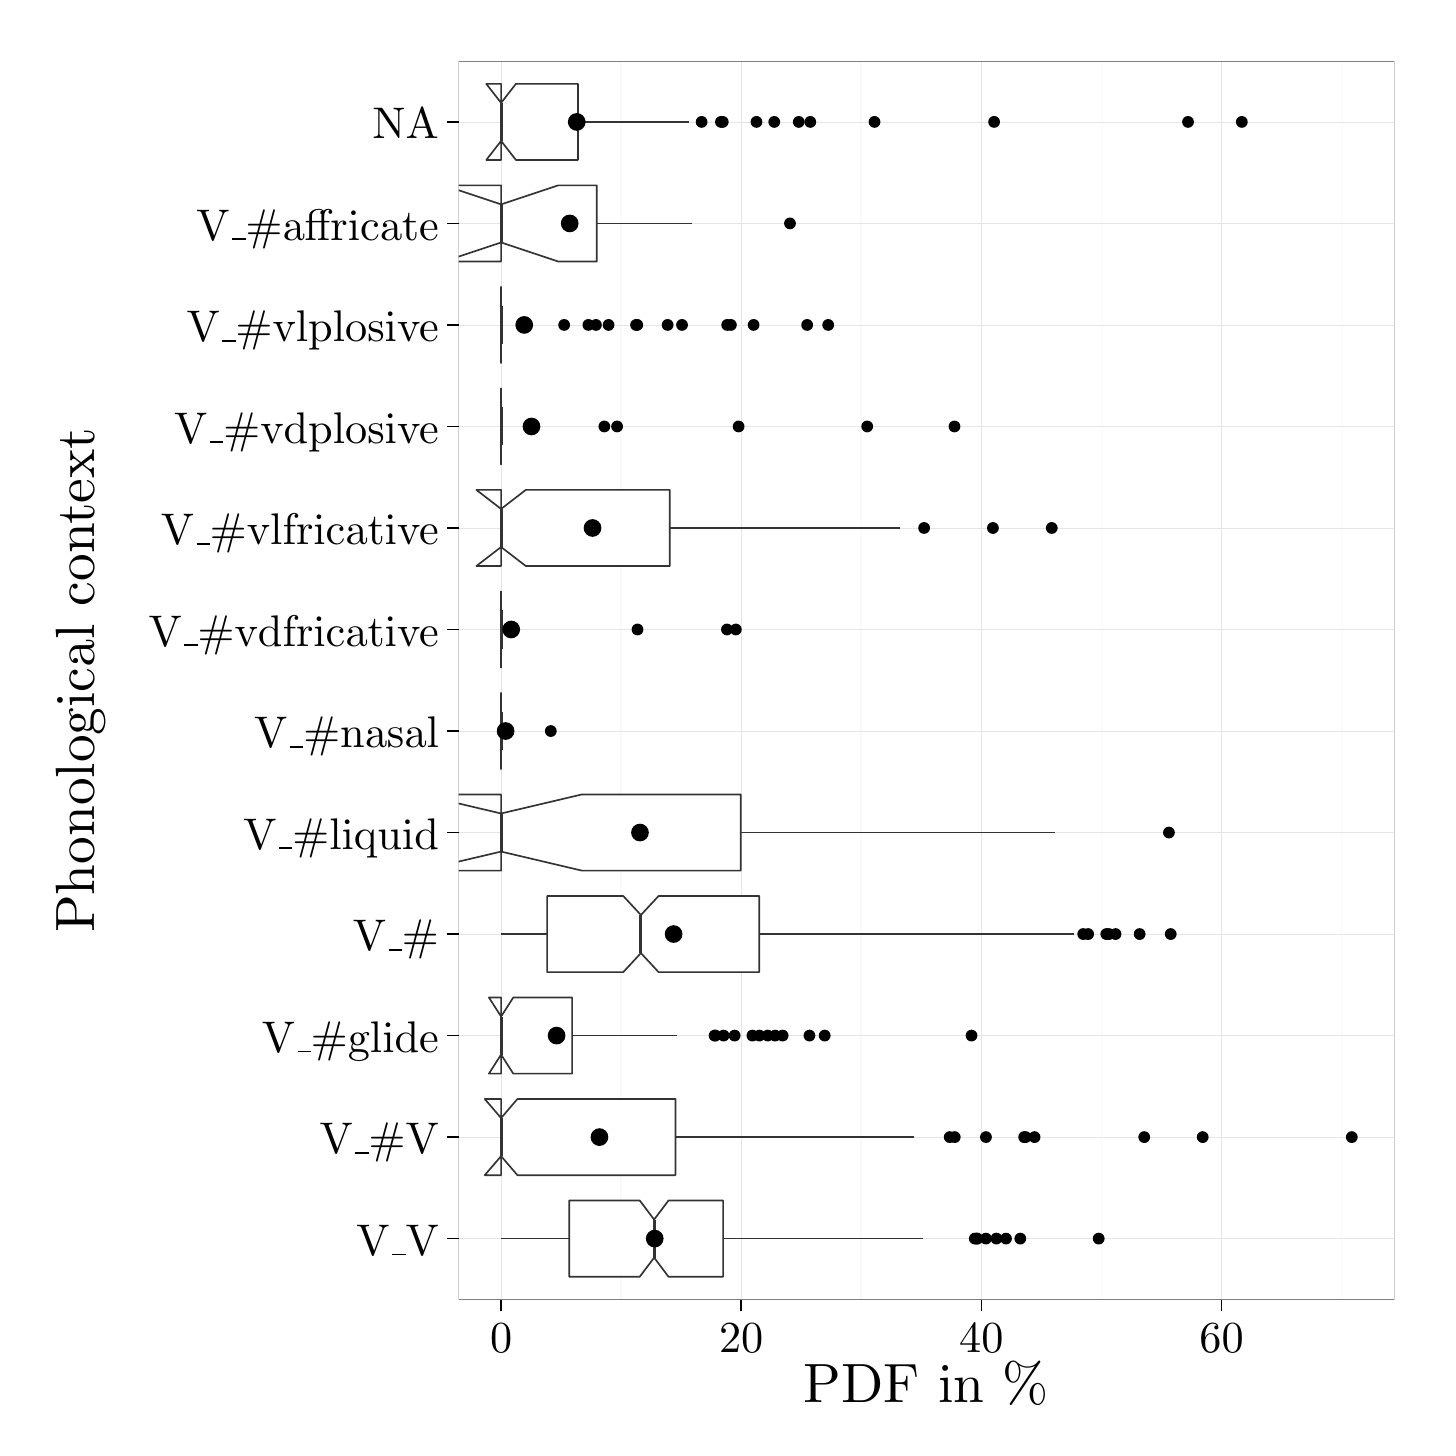
\begin{tikzpicture}[x=1pt,y=1pt]
\definecolor{fillColor}{RGB}{255,255,255}
\path[use as bounding box,fill=fillColor,fill opacity=0.00] (0,0) rectangle (505.89,505.89);
\begin{scope}
\path[clip] (  0.00,  0.00) rectangle (505.89,505.89);
\definecolor{drawColor}{RGB}{255,255,255}
\definecolor{fillColor}{RGB}{255,255,255}

\path[draw=drawColor,line width= 0.6pt,line join=round,line cap=round,fill=fillColor] (  0.00, -0.00) rectangle (505.89,505.89);
\end{scope}
\begin{scope}
\path[clip] (155.70, 46.31) rectangle (493.85,493.84);
\definecolor{fillColor}{RGB}{255,255,255}

\path[fill=fillColor] (155.70, 46.31) rectangle (493.85,493.84);
\definecolor{drawColor}{gray}{0.98}

\path[draw=drawColor,line width= 0.6pt,line join=round] (214.46, 46.31) --
	(214.46,493.84);

\path[draw=drawColor,line width= 0.6pt,line join=round] (301.23, 46.31) --
	(301.23,493.84);

\path[draw=drawColor,line width= 0.6pt,line join=round] (388.01, 46.31) --
	(388.01,493.84);

\path[draw=drawColor,line width= 0.6pt,line join=round] (474.79, 46.31) --
	(474.79,493.84);
\definecolor{drawColor}{gray}{0.90}

\path[draw=drawColor,line width= 0.2pt,line join=round] (155.70, 68.32) --
	(493.85, 68.32);

\path[draw=drawColor,line width= 0.2pt,line join=round] (155.70,105.00) --
	(493.85,105.00);

\path[draw=drawColor,line width= 0.2pt,line join=round] (155.70,141.68) --
	(493.85,141.68);

\path[draw=drawColor,line width= 0.2pt,line join=round] (155.70,178.37) --
	(493.85,178.37);

\path[draw=drawColor,line width= 0.2pt,line join=round] (155.70,215.05) --
	(493.85,215.05);

\path[draw=drawColor,line width= 0.2pt,line join=round] (155.70,251.73) --
	(493.85,251.73);

\path[draw=drawColor,line width= 0.2pt,line join=round] (155.70,288.42) --
	(493.85,288.42);

\path[draw=drawColor,line width= 0.2pt,line join=round] (155.70,325.10) --
	(493.85,325.10);

\path[draw=drawColor,line width= 0.2pt,line join=round] (155.70,361.78) --
	(493.85,361.78);

\path[draw=drawColor,line width= 0.2pt,line join=round] (155.70,398.47) --
	(493.85,398.47);

\path[draw=drawColor,line width= 0.2pt,line join=round] (155.70,435.15) --
	(493.85,435.15);

\path[draw=drawColor,line width= 0.2pt,line join=round] (155.70,471.83) --
	(493.85,471.83);

\path[draw=drawColor,line width= 0.2pt,line join=round] (171.07, 46.31) --
	(171.07,493.84);

\path[draw=drawColor,line width= 0.2pt,line join=round] (257.84, 46.31) --
	(257.84,493.84);

\path[draw=drawColor,line width= 0.2pt,line join=round] (344.62, 46.31) --
	(344.62,493.84);

\path[draw=drawColor,line width= 0.2pt,line join=round] (431.40, 46.31) --
	(431.40,493.84);
\definecolor{fillColor}{RGB}{0,0,0}

\path[fill=fillColor] (346.27, 68.32) circle (  2.13);

\path[fill=fillColor] (342.93, 68.32) circle (  2.13);

\path[fill=fillColor] (358.68, 68.32) circle (  2.13);

\path[fill=fillColor] (342.24, 68.32) circle (  2.13);

\path[fill=fillColor] (343.15, 68.32) circle (  2.13);

\path[fill=fillColor] (350.04, 68.32) circle (  2.13);

\path[fill=fillColor] (387.01, 68.32) circle (  2.13);

\path[fill=fillColor] (353.52, 68.32) circle (  2.13);
\definecolor{drawColor}{gray}{0.20}

\path[draw=drawColor,line width= 0.6pt,line join=round] (251.30, 68.32) -- (323.62, 68.32);

\path[draw=drawColor,line width= 0.6pt,line join=round] (195.67, 68.32) -- (171.07, 68.32);
\definecolor{fillColor}{RGB}{255,255,255}

\path[draw=drawColor,line width= 0.6pt,line join=round,line cap=round,fill=fillColor] (251.30, 54.56) --
	(231.55, 54.56) --
	(226.37, 61.44) --
	(221.19, 54.56) --
	(195.67, 54.56) --
	(195.67, 82.07) --
	(221.19, 82.07) --
	(226.37, 75.20) --
	(231.55, 82.07) --
	(251.30, 82.07) --
	(251.30, 54.56) --
	cycle;

\path[draw=drawColor,line width= 1.1pt,line join=round] (226.37, 61.44) -- (226.37, 75.20);
\definecolor{fillColor}{RGB}{0,0,0}

\path[fill=fillColor] (334.99,105.00) circle (  2.13);

\path[fill=fillColor] (403.46,105.00) circle (  2.13);

\path[fill=fillColor] (478.47,105.00) circle (  2.13);

\path[fill=fillColor] (360.59,105.00) circle (  2.13);

\path[fill=fillColor] (346.27,105.00) circle (  2.13);

\path[fill=fillColor] (424.59,105.00) circle (  2.13);

\path[fill=fillColor] (333.17,105.00) circle (  2.13);

\path[fill=fillColor] (360.07,105.00) circle (  2.13);

\path[fill=fillColor] (363.84,105.00) circle (  2.13);

\path[draw=drawColor,line width= 0.6pt,line join=round] (234.07,105.00) -- (320.24,105.00);

\path[draw=drawColor,line width= 0.6pt,line join=round] (171.07,105.00) -- (171.07,105.00);
\definecolor{fillColor}{RGB}{255,255,255}

\path[draw=drawColor,line width= 0.6pt,line join=round,line cap=round,fill=fillColor] (234.07, 91.24) --
	(176.97, 91.24) --
	(171.07, 98.12) --
	(165.16, 91.24) --
	(171.07, 91.24) --
	(171.07,118.76) --
	(165.16,118.76) --
	(171.07,111.88) --
	(176.97,118.76) --
	(234.07,118.76) --
	(234.07, 91.24) --
	cycle;

\path[draw=drawColor,line width= 1.1pt,line join=round] (171.07, 98.12) -- (171.07,111.88);
\definecolor{fillColor}{RGB}{0,0,0}

\path[fill=fillColor] (255.46,141.68) circle (  2.13);

\path[fill=fillColor] (251.47,141.68) circle (  2.13);

\path[fill=fillColor] (248.21,141.68) circle (  2.13);

\path[fill=fillColor] (248.52,141.68) circle (  2.13);

\path[fill=fillColor] (341.06,141.68) circle (  2.13);

\path[fill=fillColor] (272.81,141.68) circle (  2.13);

\path[fill=fillColor] (288.00,141.68) circle (  2.13);

\path[fill=fillColor] (282.49,141.68) circle (  2.13);

\path[fill=fillColor] (270.08,141.68) circle (  2.13);

\path[fill=fillColor] (267.43,141.68) circle (  2.13);

\path[fill=fillColor] (264.40,141.68) circle (  2.13);

\path[fill=fillColor] (261.88,141.68) circle (  2.13);

\path[draw=drawColor,line width= 0.6pt,line join=round] (196.75,141.68) -- (234.46,141.68);

\path[draw=drawColor,line width= 0.6pt,line join=round] (171.07,141.68) -- (171.07,141.68);
\definecolor{fillColor}{RGB}{255,255,255}

\path[draw=drawColor,line width= 0.6pt,line join=round,line cap=round,fill=fillColor] (196.75,127.93) --
	(175.47,127.93) --
	(171.07,134.81) --
	(166.67,127.93) --
	(171.07,127.93) --
	(171.07,155.44) --
	(166.67,155.44) --
	(171.07,148.56) --
	(175.47,155.44) --
	(196.75,155.44) --
	(196.75,127.93) --
	cycle;

\path[draw=drawColor,line width= 1.1pt,line join=round] (171.07,134.81) -- (171.07,148.56);
\definecolor{fillColor}{RGB}{0,0,0}

\path[fill=fillColor] (389.75,178.37) circle (  2.13);

\path[fill=fillColor] (413.04,178.37) circle (  2.13);

\path[fill=fillColor] (383.19,178.37) circle (  2.13);

\path[fill=fillColor] (381.41,178.37) circle (  2.13);

\path[fill=fillColor] (390.70,178.37) circle (  2.13);

\path[fill=fillColor] (401.81,178.37) circle (  2.13);

\path[fill=fillColor] (393.09,178.37) circle (  2.13);

\path[draw=drawColor,line width= 0.6pt,line join=round] (264.36,178.37) -- (377.94,178.37);

\path[draw=drawColor,line width= 0.6pt,line join=round] (187.71,178.37) -- (171.07,178.37);
\definecolor{fillColor}{RGB}{255,255,255}

\path[draw=drawColor,line width= 0.6pt,line join=round,line cap=round,fill=fillColor] (264.36,164.61) --
	(227.98,164.61) --
	(221.59,171.49) --
	(215.21,164.61) --
	(187.71,164.61) --
	(187.71,192.12) --
	(215.21,192.12) --
	(221.59,185.25) --
	(227.98,192.12) --
	(264.36,192.12) --
	(264.36,164.61) --
	cycle;

\path[draw=drawColor,line width= 1.1pt,line join=round] (221.59,171.49) -- (221.59,185.25);
\definecolor{fillColor}{RGB}{0,0,0}

\path[fill=fillColor] (412.39,215.05) circle (  2.13);

\path[draw=drawColor,line width= 0.6pt,line join=round] (257.68,215.05) -- (371.04,215.05);

\path[draw=drawColor,line width= 0.6pt,line join=round] (171.07,215.05) -- (171.07,215.05);
\definecolor{fillColor}{RGB}{255,255,255}

\path[draw=drawColor,line width= 0.6pt,line join=round,line cap=round,fill=fillColor] (257.68,201.29) --
	(200.24,201.29) --
	(171.07,208.17) --
	(141.89,201.29) --
	(171.07,201.29) --
	(171.07,228.81) --
	(141.89,228.81) --
	(171.07,221.93) --
	(200.24,228.81) --
	(257.68,228.81) --
	(257.68,201.29) --
	cycle;

\path[draw=drawColor,line width= 1.1pt,line join=round] (171.07,208.17) -- (171.07,221.93);
\definecolor{fillColor}{RGB}{0,0,0}

\path[fill=fillColor] (189.03,251.73) circle (  2.13);

\path[draw=drawColor,line width= 0.6pt,line join=round] (171.07,251.73) -- (171.07,251.73);

\path[draw=drawColor,line width= 0.6pt,line join=round] (171.07,251.73) -- (171.07,251.73);
\definecolor{fillColor}{RGB}{255,255,255}

\path[draw=drawColor,line width= 0.6pt,line join=round,line cap=round,fill=fillColor] (171.07,237.98) --
	(171.07,237.98) --
	(171.07,244.86) --
	(171.07,237.98) --
	(171.07,237.98) --
	(171.07,265.49) --
	(171.07,265.49) --
	(171.07,258.61) --
	(171.07,265.49) --
	(171.07,265.49) --
	(171.07,237.98) --
	cycle;

\path[draw=drawColor,line width= 1.1pt,line join=round] (171.07,244.86) -- (171.07,258.61);
\definecolor{fillColor}{RGB}{0,0,0}

\path[fill=fillColor] (220.36,288.42) circle (  2.13);

\path[fill=fillColor] (252.68,288.42) circle (  2.13);

\path[fill=fillColor] (255.89,288.42) circle (  2.13);

\path[draw=drawColor,line width= 0.6pt,line join=round] (171.07,288.42) -- (171.07,288.42);

\path[draw=drawColor,line width= 0.6pt,line join=round] (171.07,288.42) -- (171.07,288.42);
\definecolor{fillColor}{RGB}{255,255,255}

\path[draw=drawColor,line width= 0.6pt,line join=round,line cap=round,fill=fillColor] (171.07,274.66) --
	(171.07,274.66) --
	(171.07,281.54) --
	(171.07,274.66) --
	(171.07,274.66) --
	(171.07,302.17) --
	(171.07,302.17) --
	(171.07,295.30) --
	(171.07,302.17) --
	(171.07,302.17) --
	(171.07,274.66) --
	cycle;

\path[draw=drawColor,line width= 1.1pt,line join=round] (171.07,281.54) -- (171.07,295.30);
\definecolor{fillColor}{RGB}{0,0,0}

\path[fill=fillColor] (348.79,325.10) circle (  2.13);

\path[fill=fillColor] (370.05,325.10) circle (  2.13);

\path[fill=fillColor] (323.93,325.10) circle (  2.13);

\path[draw=drawColor,line width= 0.6pt,line join=round] (231.99,325.10) -- (315.03,325.10);

\path[draw=drawColor,line width= 0.6pt,line join=round] (171.07,325.10) -- (171.07,325.10);
\definecolor{fillColor}{RGB}{255,255,255}

\path[draw=drawColor,line width= 0.6pt,line join=round,line cap=round,fill=fillColor] (231.99,311.35) --
	(180.00,311.35) --
	(171.07,318.22) --
	(162.13,311.35) --
	(171.07,311.35) --
	(171.07,338.86) --
	(162.13,338.86) --
	(171.07,331.98) --
	(180.00,338.86) --
	(231.99,338.86) --
	(231.99,311.35) --
	cycle;

\path[draw=drawColor,line width= 1.1pt,line join=round] (171.07,318.22) -- (171.07,331.98);
\definecolor{fillColor}{RGB}{0,0,0}

\path[fill=fillColor] (212.98,361.78) circle (  2.13);

\path[fill=fillColor] (256.89,361.78) circle (  2.13);

\path[fill=fillColor] (208.38,361.78) circle (  2.13);

\path[fill=fillColor] (334.90,361.78) circle (  2.13);

\path[fill=fillColor] (303.36,361.78) circle (  2.13);

\path[draw=drawColor,line width= 0.6pt,line join=round] (171.07,361.78) -- (171.07,361.78);

\path[draw=drawColor,line width= 0.6pt,line join=round] (171.07,361.78) -- (171.07,361.78);
\definecolor{fillColor}{RGB}{255,255,255}

\path[draw=drawColor,line width= 0.6pt,line join=round,line cap=round,fill=fillColor] (171.07,348.03) --
	(171.07,348.03) --
	(171.07,354.91) --
	(171.07,348.03) --
	(171.07,348.03) --
	(171.07,375.54) --
	(171.07,375.54) --
	(171.07,368.66) --
	(171.07,375.54) --
	(171.07,375.54) --
	(171.07,348.03) --
	cycle;

\path[draw=drawColor,line width= 1.1pt,line join=round] (171.07,354.91) -- (171.07,368.66);
\definecolor{fillColor}{RGB}{0,0,0}

\path[fill=fillColor] (254.11,398.47) circle (  2.13);

\path[fill=fillColor] (262.31,398.47) circle (  2.13);

\path[fill=fillColor] (205.34,398.47) circle (  2.13);

\path[fill=fillColor] (231.25,398.47) circle (  2.13);

\path[fill=fillColor] (202.61,398.47) circle (  2.13);

\path[fill=fillColor] (193.85,398.47) circle (  2.13);

\path[fill=fillColor] (252.77,398.47) circle (  2.13);

\path[fill=fillColor] (281.66,398.47) circle (  2.13);

\path[fill=fillColor] (219.84,398.47) circle (  2.13);

\path[fill=fillColor] (289.26,398.47) circle (  2.13);

\path[fill=fillColor] (209.90,398.47) circle (  2.13);

\path[fill=fillColor] (236.45,398.47) circle (  2.13);

\path[fill=fillColor] (220.27,398.47) circle (  2.13);

\path[draw=drawColor,line width= 0.6pt,line join=round] (171.07,398.47) -- (171.07,398.47);

\path[draw=drawColor,line width= 0.6pt,line join=round] (171.07,398.47) -- (171.07,398.47);
\definecolor{fillColor}{RGB}{255,255,255}

\path[draw=drawColor,line width= 0.6pt,line join=round,line cap=round,fill=fillColor] (171.07,384.71) --
	(171.07,384.71) --
	(171.07,391.59) --
	(171.07,384.71) --
	(171.07,384.71) --
	(171.07,412.22) --
	(171.07,412.22) --
	(171.07,405.35) --
	(171.07,412.22) --
	(171.07,412.22) --
	(171.07,384.71) --
	cycle;

\path[draw=drawColor,line width= 1.1pt,line join=round] (171.07,391.59) -- (171.07,405.35);
\definecolor{fillColor}{RGB}{0,0,0}

\path[fill=fillColor] (275.46,435.15) circle (  2.13);

\path[draw=drawColor,line width= 0.6pt,line join=round] (205.65,435.15) -- (240.23,435.15);

\path[draw=drawColor,line width= 0.6pt,line join=round] (171.07,435.15) -- (171.07,435.15);
\definecolor{fillColor}{RGB}{255,255,255}

\path[draw=drawColor,line width= 0.6pt,line join=round,line cap=round,fill=fillColor] (205.65,421.40) --
	(191.72,421.40) --
	(171.07,428.27) --
	(150.42,421.40) --
	(171.07,421.40) --
	(171.07,448.91) --
	(150.42,448.91) --
	(171.07,442.03) --
	(191.72,448.91) --
	(205.65,448.91) --
	(205.65,421.40) --
	cycle;

\path[draw=drawColor,line width= 1.1pt,line join=round] (171.07,428.27) -- (171.07,442.03);
\definecolor{fillColor}{RGB}{0,0,0}

\path[fill=fillColor] (278.63,471.83) circle (  2.13);

\path[fill=fillColor] (306.01,471.83) circle (  2.13);

\path[fill=fillColor] (243.53,471.83) circle (  2.13);

\path[fill=fillColor] (250.51,471.83) circle (  2.13);

\path[fill=fillColor] (419.29,471.83) circle (  2.13);

\path[fill=fillColor] (251.16,471.83) circle (  2.13);

\path[fill=fillColor] (349.22,471.83) circle (  2.13);

\path[fill=fillColor] (438.73,471.83) circle (  2.13);

\path[fill=fillColor] (263.35,471.83) circle (  2.13);

\path[fill=fillColor] (282.79,471.83) circle (  2.13);

\path[fill=fillColor] (269.78,471.83) circle (  2.13);

\path[draw=drawColor,line width= 0.6pt,line join=round] (198.84,471.83) -- (238.84,471.83);

\path[draw=drawColor,line width= 0.6pt,line join=round] (171.07,471.83) -- (171.07,471.83);
\definecolor{fillColor}{RGB}{255,255,255}

\path[draw=drawColor,line width= 0.6pt,line join=round,line cap=round,fill=fillColor] (198.84,458.08) --
	(176.43,458.08) --
	(171.07,464.96) --
	(165.71,458.08) --
	(171.07,458.08) --
	(171.07,485.59) --
	(165.71,485.59) --
	(171.07,478.71) --
	(176.43,485.59) --
	(198.84,485.59) --
	(198.84,458.08) --
	cycle;

\path[draw=drawColor,line width= 1.1pt,line join=round] (171.07,464.96) -- (171.07,478.71);
\definecolor{fillColor}{RGB}{0,0,0}

\path[fill=fillColor] (226.58, 68.32) circle (  3.20);

\path[fill=fillColor] (179.43,398.47) circle (  3.20);

\path[fill=fillColor] (195.86,435.15) circle (  3.20);

\path[fill=fillColor] (198.40,471.83) circle (  3.20);

\path[fill=fillColor] (206.61,105.00) circle (  3.20);

\path[fill=fillColor] (191.12,141.68) circle (  3.20);

\path[fill=fillColor] (233.41,178.37) circle (  3.20);

\path[fill=fillColor] (221.25,215.05) circle (  3.20);

\path[fill=fillColor] (172.70,251.73) circle (  3.20);

\path[fill=fillColor] (174.72,288.42) circle (  3.20);

\path[fill=fillColor] (204.11,325.10) circle (  3.20);

\path[fill=fillColor] (182.05,361.78) circle (  3.20);
\definecolor{drawColor}{gray}{0.50}

\path[draw=drawColor,line width= 0.6pt,line join=round,line cap=round] (155.70, 46.31) rectangle (493.85,493.84);
\end{scope}
\begin{scope}
\path[clip] (  0.00,  0.00) rectangle (505.89,505.89);
\definecolor{drawColor}{RGB}{0,0,0}

\node[text=drawColor,anchor=base east,inner sep=0pt, outer sep=0pt, scale=  1.60] at (148.58, 62.28) {V{\_{}}V};

\node[text=drawColor,anchor=base east,inner sep=0pt, outer sep=0pt, scale=  1.60] at (148.58, 98.97) {V{\_{}}{\#}V};

\node[text=drawColor,anchor=base east,inner sep=0pt, outer sep=0pt, scale=  1.60] at (148.58,135.65) {V{\_{}}{\#}glide};

\node[text=drawColor,anchor=base east,inner sep=0pt, outer sep=0pt, scale=  1.60] at (148.58,172.33) {V{\_{}}{\#}};

\node[text=drawColor,anchor=base east,inner sep=0pt, outer sep=0pt, scale=  1.60] at (148.58,209.02) {V{\_{}}{\#}liquid};

\node[text=drawColor,anchor=base east,inner sep=0pt, outer sep=0pt, scale=  1.60] at (148.58,245.70) {V{\_{}}{\#}nasal};

\node[text=drawColor,anchor=base east,inner sep=0pt, outer sep=0pt, scale=  1.60] at (148.58,282.38) {V{\_{}}{\#}vdfricative};

\node[text=drawColor,anchor=base east,inner sep=0pt, outer sep=0pt, scale=  1.60] at (148.58,319.07) {V{\_{}}{\#}vlfricative};

\node[text=drawColor,anchor=base east,inner sep=0pt, outer sep=0pt, scale=  1.60] at (148.58,355.75) {V{\_{}}{\#}vdplosive};

\node[text=drawColor,anchor=base east,inner sep=0pt, outer sep=0pt, scale=  1.60] at (148.58,392.43) {V{\_{}}{\#}vlplosive};

\node[text=drawColor,anchor=base east,inner sep=0pt, outer sep=0pt, scale=  1.60] at (148.58,429.12) {V{\_{}}{\#}affricate};

\node[text=drawColor,anchor=base east,inner sep=0pt, outer sep=0pt, scale=  1.60] at (148.58,465.80) {NA};
\end{scope}
\begin{scope}
\path[clip] (  0.00,  0.00) rectangle (505.89,505.89);
\definecolor{drawColor}{RGB}{0,0,0}

\path[draw=drawColor,line width= 0.6pt,line join=round] (151.43, 68.32) --
	(155.70, 68.32);

\path[draw=drawColor,line width= 0.6pt,line join=round] (151.43,105.00) --
	(155.70,105.00);

\path[draw=drawColor,line width= 0.6pt,line join=round] (151.43,141.68) --
	(155.70,141.68);

\path[draw=drawColor,line width= 0.6pt,line join=round] (151.43,178.37) --
	(155.70,178.37);

\path[draw=drawColor,line width= 0.6pt,line join=round] (151.43,215.05) --
	(155.70,215.05);

\path[draw=drawColor,line width= 0.6pt,line join=round] (151.43,251.73) --
	(155.70,251.73);

\path[draw=drawColor,line width= 0.6pt,line join=round] (151.43,288.42) --
	(155.70,288.42);

\path[draw=drawColor,line width= 0.6pt,line join=round] (151.43,325.10) --
	(155.70,325.10);

\path[draw=drawColor,line width= 0.6pt,line join=round] (151.43,361.78) --
	(155.70,361.78);

\path[draw=drawColor,line width= 0.6pt,line join=round] (151.43,398.47) --
	(155.70,398.47);

\path[draw=drawColor,line width= 0.6pt,line join=round] (151.43,435.15) --
	(155.70,435.15);

\path[draw=drawColor,line width= 0.6pt,line join=round] (151.43,471.83) --
	(155.70,471.83);
\end{scope}
\begin{scope}
\path[clip] (  0.00,  0.00) rectangle (505.89,505.89);
\definecolor{drawColor}{RGB}{0,0,0}

\path[draw=drawColor,line width= 0.6pt,line join=round] (171.07, 42.04) --
	(171.07, 46.31);

\path[draw=drawColor,line width= 0.6pt,line join=round] (257.84, 42.04) --
	(257.84, 46.31);

\path[draw=drawColor,line width= 0.6pt,line join=round] (344.62, 42.04) --
	(344.62, 46.31);

\path[draw=drawColor,line width= 0.6pt,line join=round] (431.40, 42.04) --
	(431.40, 46.31);
\end{scope}
\begin{scope}
\path[clip] (  0.00,  0.00) rectangle (505.89,505.89);
\definecolor{drawColor}{RGB}{0,0,0}

\node[text=drawColor,anchor=base,inner sep=0pt, outer sep=0pt, scale=  1.60] at (171.07, 27.13) {0};

\node[text=drawColor,anchor=base,inner sep=0pt, outer sep=0pt, scale=  1.60] at (257.84, 27.13) {20};

\node[text=drawColor,anchor=base,inner sep=0pt, outer sep=0pt, scale=  1.60] at (344.62, 27.13) {40};

\node[text=drawColor,anchor=base,inner sep=0pt, outer sep=0pt, scale=  1.60] at (431.40, 27.13) {60};
\end{scope}
\begin{scope}
\path[clip] (  0.00,  0.00) rectangle (505.89,505.89);
\definecolor{drawColor}{RGB}{0,0,0}

\node[text=drawColor,anchor=base,inner sep=0pt, outer sep=0pt, scale=  2.00] at (324.77,  9.03) {PDF in {\%}};
\end{scope}
\begin{scope}
\path[clip] (  0.00,  0.00) rectangle (505.89,505.89);
\definecolor{drawColor}{RGB}{0,0,0}

\node[text=drawColor,rotate= 90.00,anchor=base,inner sep=0pt, outer sep=0pt, scale=  2.00] at ( 24.12,270.08) {Phonological context};
\end{scope}
\end{tikzpicture}
} 
	\caption{/ŋ(g)/: PDF by phonological environment (without [ɪn] realisations)}
	\label{fig.box.ng.environment}
\end{figure}

\figref{fig.box.ng.environment} is a box plot that visualises \isi{PDF} of /ŋ(g)/ for the different \isi{phonological context}s separately.
``NA'' refers to instances of /ŋ(g)/ that occurred in words for which no phonemic transcription was available -- mostly proper names -- and which were therefore not coded for phonological environment\is{phonological context}.
These (67) cases will not be discussed here any further.
The remaining contexts seem to fall into three groups (cf. \tabref{tab.ng.mean.environment} for the exact means):
\begin{inparaenum}[(1)]
	\item Comparatively high \isi{PDF} (word-final\is{phonological context}, intervocalic\is{phonological context}, followed by liquids),
	\item medium \isi{PDF} (intervocalic\is{phonological context} across word-boundary, followed by voiceless fricatives), and
	\item low \isi{PDF} (followed by stops, voiced fricatives, and glides).
\end{inparaenum}
The last group has mean \isi{PDF} values that are close to 0.
The box plot visualises that the median (thick vertical bar) is often 0 as well in these contexts (cf., for instance, ``V\_\#affricate'' or ``V\_\#glide''), which means that at least 50\% of observations in this category have a \isi{PDF} of 0, i.e. they are realised by a (standard) [ŋ].
For phonological environment\is{phonological context}s such as ``V\_\#nasal'' or ``V\_\#vdfricative'' no box (in the everyday sense) is generated at all, because the first, second, \emph{and} the third quantile are 0 -- the realisation as [ŋ] thus accounts for 75+\% of cases in these categories.

\begin{table}[h]
	\centering
	\caption{/ŋ(g)/: PDF means by phonological environment ([ɪn] excluded)}
	\label{tab.ng.mean.environment}
	\begin{tabular}{lrr}
		\toprule
		environment & mean \isi{PDF} & n\\
		\midrule
		V\_V & 12.79 & 288\\
		V\_\#V & 8.19 & 284\\
		V\_\#glide & 4.62 & 85\\
		V\_\# & 14.37 & 360\\
		V\_\#liquid & 11.57 & 22\\
		V\_\#nasal & 0.38 & 11\\
		V\_\#voiced fricative & 0.84 & 59\\
		V\_\#voiceless fricative & 7.62 & 116\\
		V\_\#voiced plosive & 2.53 & 42\\
		V\_\#voiceless plosive & 1.93 & 100\\
		V\_\#affricate & 5.71 & 7\\
		\bottomrule
	\end{tabular}
\end{table}

It should be noted, however, that almost \emph{all} environments have a median \isi{PDF} of 0.
The only exceptions are cases where velar nasal plus occurs intervocalic\is{phonological context}ally within a word or in phrase final position (``V\_\#''), i.e. when the variable is followed by silence.
In these environments, some sort of plosive was observed in more than 75\% of cases (the first quantile is greater than 0 for both categories).
This clearly sets them apart from the remaining contexts, because in the former velar nasal plus seems to be the norm (at least in my sample), whereas in the latter it is an option, but not -- statistically speaking -- the default one.
Having said that, two caveats need to be mentioned.
Firstly, the amount of data that are available for each context varies greatly (cf. \tabref{tab.ng.mean.environment}): while there is a rather sound basis for ``V\_V'', ``V\_\#V'', and ``V\_\#'', only 11 (7) observations in the sample, for instance, represent contexts where velar nasal plus is followed by a nasal (affricate).
Secondly, only the two environments `intervocalic\is{phonological context}' (within a word) and `word-final\is{phonological context}' (pre-pausal) occur in the word list.
It is therefore possible that the high mean \isi{PDF} values for these environments are at least in part due to their occurrence in the most formal speech style (the relationship between velar nasal plus and careful speech is addressed below).

This fact would constitute a problem if the present study was primarily concerned with identifying and describing the influence (on the realisation of /ŋ(g)/) of different \isi{phonological context}s.
The focus, however, is on the social predictors on the one hand, and style on the other.
Additionally, the intervocalic\is{phonological context} (within word) and word-final\is{phonological context} contexts are rather prominent in the sample \emph{generally}.
Together with intervocalic\is{phonological context} (across a word-boundary), an environment that is just as frequent as intervocalic\is{phonological context} (within word) and which also has a comparatively high mean \isi{PDF}, these two contexts  already account for 68.03\% of the /ŋ(g)/ observations ([ɪn] realisations excluded).
Crucially, `V\_V' and `V\_\#' occur in \emph{all} styles investigated and in roughly equal proportions (with the notable exception of the word list, as explained above).
Thus, they dominate the sample by their sheer numbers, but they do not distort it by biasing it towards a particular (formal) register.
It is, however, possible that \isi{PDF} values calculated for the word list are higher than they would be if velar nasal plus had been elicited in more contexts in addition to the two `plosive-favouring' ones.

\subsection{Style and gender}
\label{sec.prod.res.con.ng.stylegender}

\begin{figure}[h]
	\centering
		\definecolor{shadecolor}{rgb}{0.969, 0.969, 0.969}
		\resizebox{.49\linewidth}{!}{% Created by tikzDevice version 0.8.1 on 2016-02-09 02:16:47
% !TEX encoding = UTF-8 Unicode
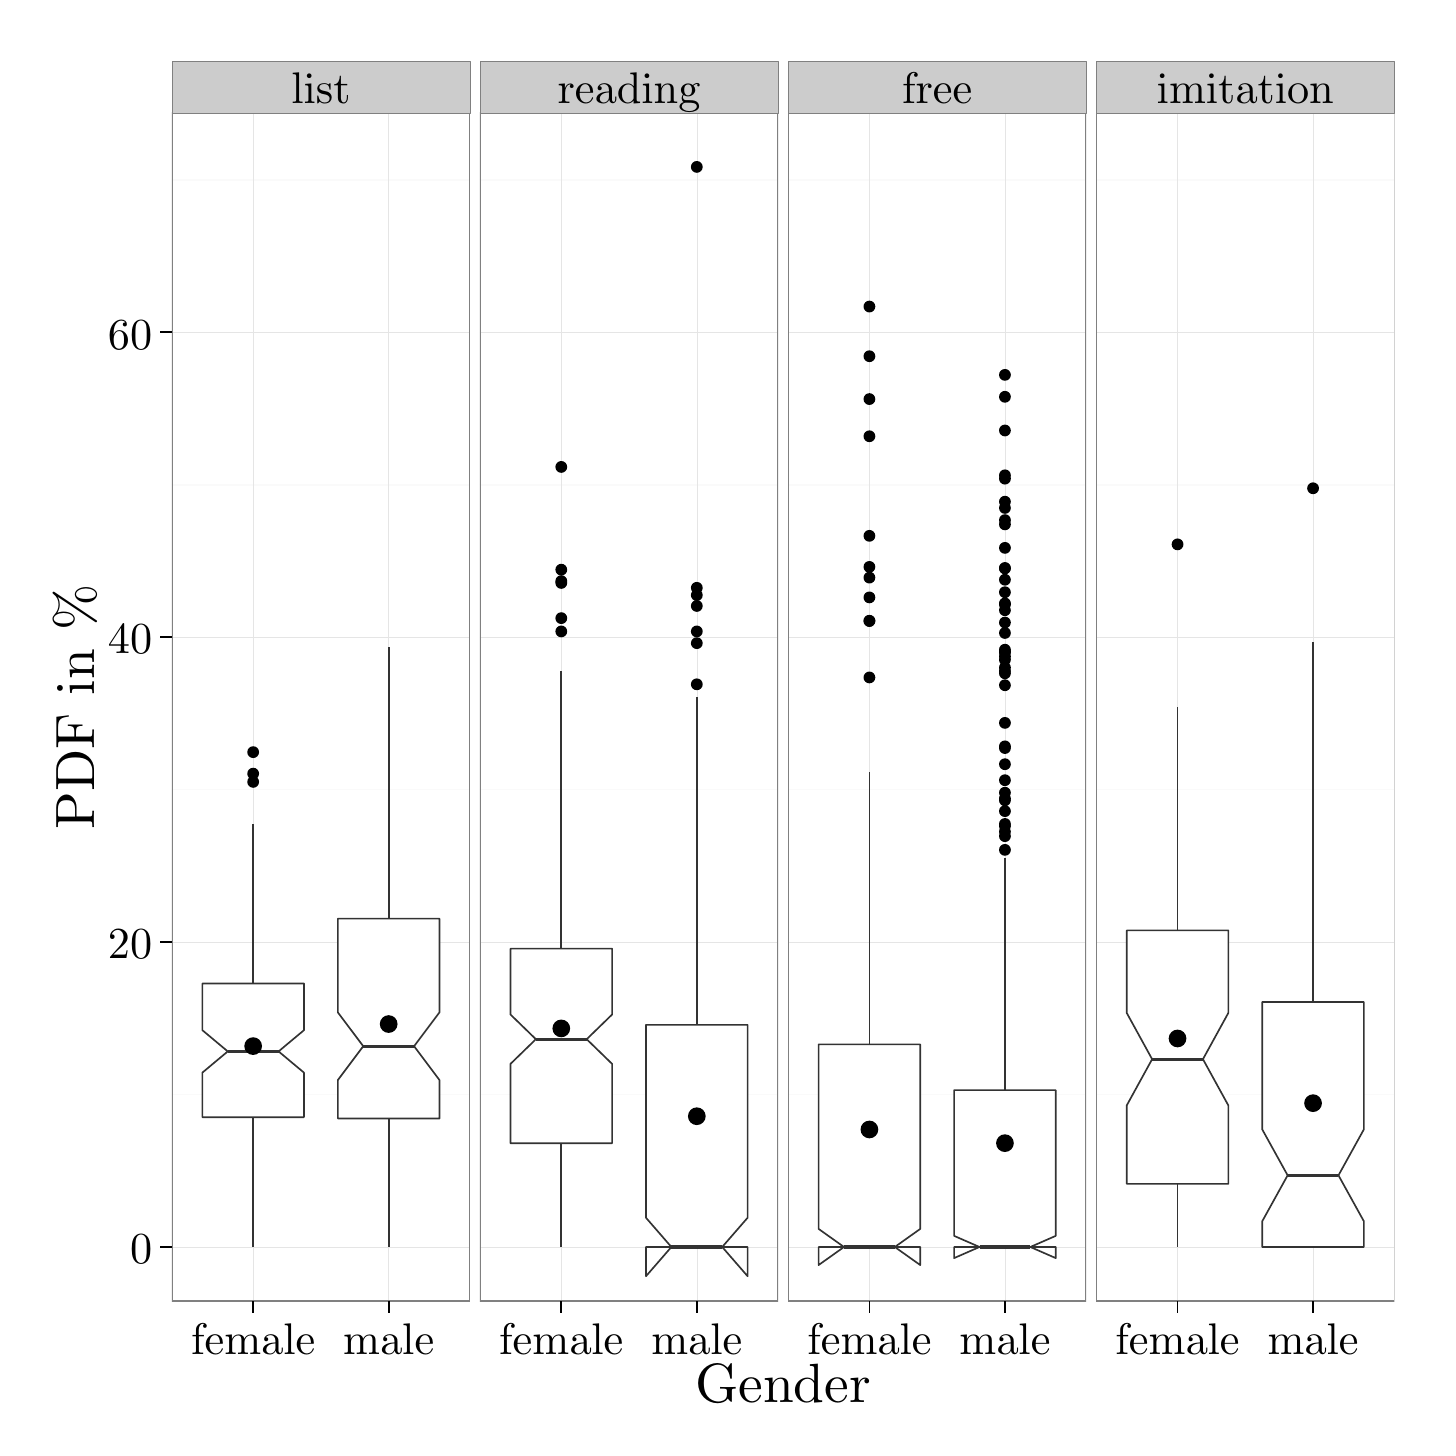
\begin{tikzpicture}[x=1pt,y=1pt]
\definecolor{fillColor}{RGB}{255,255,255}
\path[use as bounding box,fill=fillColor,fill opacity=0.00] (0,0) rectangle (505.89,505.89);
\begin{scope}
\path[clip] (  0.00,  0.00) rectangle (505.89,505.89);
\definecolor{drawColor}{RGB}{255,255,255}
\definecolor{fillColor}{RGB}{255,255,255}

\path[draw=drawColor,line width= 0.6pt,line join=round,line cap=round,fill=fillColor] (  0.00, -0.00) rectangle (505.89,505.89);
\end{scope}
\begin{scope}
\path[clip] ( 52.10, 45.77) rectangle (159.83,475.09);
\definecolor{fillColor}{RGB}{255,255,255}

\path[fill=fillColor] ( 52.10, 45.77) rectangle (159.83,475.09);
\definecolor{drawColor}{gray}{0.98}

\path[draw=drawColor,line width= 0.6pt,line join=round] ( 52.10,120.37) --
	(159.83,120.37);

\path[draw=drawColor,line width= 0.6pt,line join=round] ( 52.10,230.55) --
	(159.83,230.55);

\path[draw=drawColor,line width= 0.6pt,line join=round] ( 52.10,340.72) --
	(159.83,340.72);

\path[draw=drawColor,line width= 0.6pt,line join=round] ( 52.10,450.89) --
	(159.83,450.89);
\definecolor{drawColor}{gray}{0.90}

\path[draw=drawColor,line width= 0.2pt,line join=round] ( 52.10, 65.29) --
	(159.83, 65.29);

\path[draw=drawColor,line width= 0.2pt,line join=round] ( 52.10,175.46) --
	(159.83,175.46);

\path[draw=drawColor,line width= 0.2pt,line join=round] ( 52.10,285.63) --
	(159.83,285.63);

\path[draw=drawColor,line width= 0.2pt,line join=round] ( 52.10,395.80) --
	(159.83,395.80);

\path[draw=drawColor,line width= 0.2pt,line join=round] ( 81.48, 45.77) --
	( 81.48,475.09);

\path[draw=drawColor,line width= 0.2pt,line join=round] (130.45, 45.77) --
	(130.45,475.09);
\definecolor{fillColor}{RGB}{0,0,0}

\path[fill=fillColor] ( 81.48,233.35) circle (  2.13);

\path[fill=fillColor] ( 81.48,236.33) circle (  2.13);

\path[fill=fillColor] ( 81.48,244.10) circle (  2.13);
\definecolor{drawColor}{gray}{0.20}

\path[draw=drawColor,line width= 0.6pt,line join=round] ( 81.48,160.50) -- ( 81.48,218.21);

\path[draw=drawColor,line width= 0.6pt,line join=round] ( 81.48,112.19) -- ( 81.48, 65.29);
\definecolor{fillColor}{RGB}{255,255,255}

\path[draw=drawColor,line width= 0.6pt,line join=round,line cap=round,fill=fillColor] ( 63.12,160.50) --
	( 63.12,143.63) --
	( 72.30,135.96) --
	( 63.12,128.29) --
	( 63.12,112.19) --
	( 99.84,112.19) --
	( 99.84,128.29) --
	( 90.66,135.96) --
	( 99.84,143.63) --
	( 99.84,160.50) --
	( 63.12,160.50) --
	cycle;

\path[draw=drawColor,line width= 1.1pt,line join=round] ( 72.30,135.96) -- ( 90.66,135.96);

\path[draw=drawColor,line width= 0.6pt,line join=round] (130.45,183.94) -- (130.45,282.22);

\path[draw=drawColor,line width= 0.6pt,line join=round] (130.45,111.72) -- (130.45, 65.29);

\path[draw=drawColor,line width= 0.6pt,line join=round,line cap=round,fill=fillColor] (112.08,183.94) --
	(112.08,150.07) --
	(121.26,137.84) --
	(112.08,125.60) --
	(112.08,111.72) --
	(148.81,111.72) --
	(148.81,125.60) --
	(139.63,137.84) --
	(148.81,150.07) --
	(148.81,183.94) --
	(112.08,183.94) --
	cycle;

\path[draw=drawColor,line width= 1.1pt,line join=round] (121.26,137.84) -- (139.63,137.84);
\definecolor{fillColor}{RGB}{0,0,0}

\path[fill=fillColor] ( 81.48,137.88) circle (  3.20);

\path[fill=fillColor] (130.45,145.85) circle (  3.20);
\definecolor{drawColor}{gray}{0.50}

\path[draw=drawColor,line width= 0.6pt,line join=round,line cap=round] ( 52.10, 45.77) rectangle (159.83,475.09);
\end{scope}
\begin{scope}
\path[clip] (163.44, 45.77) rectangle (271.17,475.09);
\definecolor{fillColor}{RGB}{255,255,255}

\path[fill=fillColor] (163.44, 45.77) rectangle (271.17,475.09);
\definecolor{drawColor}{gray}{0.98}

\path[draw=drawColor,line width= 0.6pt,line join=round] (163.44,120.37) --
	(271.17,120.37);

\path[draw=drawColor,line width= 0.6pt,line join=round] (163.44,230.55) --
	(271.17,230.55);

\path[draw=drawColor,line width= 0.6pt,line join=round] (163.44,340.72) --
	(271.17,340.72);

\path[draw=drawColor,line width= 0.6pt,line join=round] (163.44,450.89) --
	(271.17,450.89);
\definecolor{drawColor}{gray}{0.90}

\path[draw=drawColor,line width= 0.2pt,line join=round] (163.44, 65.29) --
	(271.17, 65.29);

\path[draw=drawColor,line width= 0.2pt,line join=round] (163.44,175.46) --
	(271.17,175.46);

\path[draw=drawColor,line width= 0.2pt,line join=round] (163.44,285.63) --
	(271.17,285.63);

\path[draw=drawColor,line width= 0.2pt,line join=round] (163.44,395.80) --
	(271.17,395.80);

\path[draw=drawColor,line width= 0.2pt,line join=round] (192.82, 45.77) --
	(192.82,475.09);

\path[draw=drawColor,line width= 0.2pt,line join=round] (241.79, 45.77) --
	(241.79,475.09);
\definecolor{fillColor}{RGB}{0,0,0}

\path[fill=fillColor] (192.82,305.90) circle (  2.13);

\path[fill=fillColor] (192.82,287.72) circle (  2.13);

\path[fill=fillColor] (192.82,292.52) circle (  2.13);

\path[fill=fillColor] (192.82,305.24) circle (  2.13);

\path[fill=fillColor] (192.82,347.16) circle (  2.13);

\path[fill=fillColor] (192.82,310.03) circle (  2.13);
\definecolor{drawColor}{gray}{0.20}

\path[draw=drawColor,line width= 0.6pt,line join=round] (192.82,173.09) -- (192.82,273.29);

\path[draw=drawColor,line width= 0.6pt,line join=round] (192.82,102.80) -- (192.82, 65.29);
\definecolor{fillColor}{RGB}{255,255,255}

\path[draw=drawColor,line width= 0.6pt,line join=round,line cap=round,fill=fillColor] (174.46,173.09) --
	(174.46,149.29) --
	(183.64,140.37) --
	(174.46,131.45) --
	(174.46,102.80) --
	(211.18,102.80) --
	(211.18,131.45) --
	(202.00,140.37) --
	(211.18,149.29) --
	(211.18,173.09) --
	(174.46,173.09) --
	cycle;

\path[draw=drawColor,line width= 1.1pt,line join=round] (183.64,140.37) -- (202.00,140.37);
\definecolor{fillColor}{RGB}{0,0,0}

\path[fill=fillColor] (241.79,287.72) circle (  2.13);

\path[fill=fillColor] (241.79,283.48) circle (  2.13);

\path[fill=fillColor] (241.79,303.48) circle (  2.13);

\path[fill=fillColor] (241.79,300.84) circle (  2.13);

\path[fill=fillColor] (241.79,455.57) circle (  2.13);

\path[fill=fillColor] (241.79,268.61) circle (  2.13);

\path[fill=fillColor] (241.79,296.92) circle (  2.13);

\path[draw=drawColor,line width= 0.6pt,line join=round] (241.79,145.56) -- (241.79,263.98);

\path[draw=drawColor,line width= 0.6pt,line join=round] (241.79, 65.29) -- (241.79, 65.29);
\definecolor{fillColor}{RGB}{255,255,255}

\path[draw=drawColor,line width= 0.6pt,line join=round,line cap=round,fill=fillColor] (223.42,145.56) --
	(223.42, 75.86) --
	(232.60, 65.29) --
	(223.42, 54.72) --
	(223.42, 65.29) --
	(260.15, 65.29) --
	(260.15, 54.72) --
	(250.97, 65.29) --
	(260.15, 75.86) --
	(260.15,145.56) --
	(223.42,145.56) --
	cycle;

\path[draw=drawColor,line width= 1.1pt,line join=round] (232.60, 65.29) -- (250.97, 65.29);
\definecolor{fillColor}{RGB}{0,0,0}

\path[fill=fillColor] (192.82,144.27) circle (  3.20);

\path[fill=fillColor] (241.79,112.54) circle (  3.20);
\definecolor{drawColor}{gray}{0.50}

\path[draw=drawColor,line width= 0.6pt,line join=round,line cap=round] (163.44, 45.77) rectangle (271.17,475.09);
\end{scope}
\begin{scope}
\path[clip] (274.78, 45.77) rectangle (382.51,475.09);
\definecolor{fillColor}{RGB}{255,255,255}

\path[fill=fillColor] (274.78, 45.77) rectangle (382.51,475.09);
\definecolor{drawColor}{gray}{0.98}

\path[draw=drawColor,line width= 0.6pt,line join=round] (274.78,120.37) --
	(382.51,120.37);

\path[draw=drawColor,line width= 0.6pt,line join=round] (274.78,230.55) --
	(382.51,230.55);

\path[draw=drawColor,line width= 0.6pt,line join=round] (274.78,340.72) --
	(382.51,340.72);

\path[draw=drawColor,line width= 0.6pt,line join=round] (274.78,450.89) --
	(382.51,450.89);
\definecolor{drawColor}{gray}{0.90}

\path[draw=drawColor,line width= 0.2pt,line join=round] (274.78, 65.29) --
	(382.51, 65.29);

\path[draw=drawColor,line width= 0.2pt,line join=round] (274.78,175.46) --
	(382.51,175.46);

\path[draw=drawColor,line width= 0.2pt,line join=round] (274.78,285.63) --
	(382.51,285.63);

\path[draw=drawColor,line width= 0.2pt,line join=round] (274.78,395.80) --
	(382.51,395.80);

\path[draw=drawColor,line width= 0.2pt,line join=round] (304.16, 45.77) --
	(304.16,475.09);

\path[draw=drawColor,line width= 0.2pt,line join=round] (353.13, 45.77) --
	(353.13,475.09);
\definecolor{fillColor}{RGB}{0,0,0}

\path[fill=fillColor] (304.16,291.58) circle (  2.13);

\path[fill=fillColor] (304.16,322.26) circle (  2.13);

\path[fill=fillColor] (304.16,387.16) circle (  2.13);

\path[fill=fillColor] (304.16,358.24) circle (  2.13);

\path[fill=fillColor] (304.16,291.47) circle (  2.13);

\path[fill=fillColor] (304.16,405.11) circle (  2.13);

\path[fill=fillColor] (304.16,371.68) circle (  2.13);

\path[fill=fillColor] (304.16,271.09) circle (  2.13);

\path[fill=fillColor] (304.16,307.17) circle (  2.13);

\path[fill=fillColor] (304.16,300.01) circle (  2.13);

\path[fill=fillColor] (304.16,311.03) circle (  2.13);
\definecolor{drawColor}{gray}{0.20}

\path[draw=drawColor,line width= 0.6pt,line join=round] (304.16,138.51) -- (304.16,236.94);

\path[draw=drawColor,line width= 0.6pt,line join=round] (304.16, 65.29) -- (304.16, 65.29);
\definecolor{fillColor}{RGB}{255,255,255}

\path[draw=drawColor,line width= 0.6pt,line join=round,line cap=round,fill=fillColor] (285.80,138.51) --
	(285.80, 71.82) --
	(294.98, 65.29) --
	(285.80, 58.76) --
	(285.80, 65.29) --
	(322.52, 65.29) --
	(322.52, 58.76) --
	(313.34, 65.29) --
	(322.52, 71.82) --
	(322.52,138.51) --
	(285.80,138.51) --
	cycle;

\path[draw=drawColor,line width= 1.1pt,line join=round] (294.98, 65.29) -- (313.34, 65.29);
\definecolor{fillColor}{RGB}{0,0,0}

\path[fill=fillColor] (353.13,217.38) circle (  2.13);

\path[fill=fillColor] (353.13,226.69) circle (  2.13);

\path[fill=fillColor] (353.13,208.79) circle (  2.13);

\path[fill=fillColor] (353.13,272.58) circle (  2.13);

\path[fill=fillColor] (353.13,277.48) circle (  2.13);

\path[fill=fillColor] (353.13,254.67) circle (  2.13);

\path[fill=fillColor] (353.13,273.40) circle (  2.13);

\path[fill=fillColor] (353.13,310.48) circle (  2.13);

\path[fill=fillColor] (353.13,280.29) circle (  2.13);

\path[fill=fillColor] (353.13,245.58) circle (  2.13);

\path[fill=fillColor] (353.13,246.19) circle (  2.13);

\path[fill=fillColor] (353.13,301.88) circle (  2.13);

\path[fill=fillColor] (353.13,380.43) circle (  2.13);

\path[fill=fillColor] (353.13,342.92) circle (  2.13);

\path[fill=fillColor] (353.13,290.92) circle (  2.13);

\path[fill=fillColor] (353.13,372.50) circle (  2.13);

\path[fill=fillColor] (353.13,274.67) circle (  2.13);

\path[fill=fillColor] (353.13,334.60) circle (  2.13);

\path[fill=fillColor] (353.13,310.64) circle (  2.13);

\path[fill=fillColor] (353.13,222.78) circle (  2.13);

\path[fill=fillColor] (353.13,327.94) circle (  2.13);

\path[fill=fillColor] (353.13,287.17) circle (  2.13);

\path[fill=fillColor] (353.13,227.35) circle (  2.13);

\path[fill=fillColor] (353.13,360.33) circle (  2.13);

\path[fill=fillColor] (353.13,281.11) circle (  2.13);

\path[fill=fillColor] (353.13,239.74) circle (  2.13);

\path[fill=fillColor] (353.13,229.44) circle (  2.13);

\path[fill=fillColor] (353.13,218.15) circle (  2.13);

\path[fill=fillColor] (353.13,297.86) circle (  2.13);

\path[fill=fillColor] (353.13,306.40) circle (  2.13);

\path[fill=fillColor] (353.13,317.91) circle (  2.13);

\path[fill=fillColor] (353.13,268.28) circle (  2.13);

\path[fill=fillColor] (353.13,332.34) circle (  2.13);

\path[fill=fillColor] (353.13,295.38) circle (  2.13);

\path[fill=fillColor] (353.13,297.48) circle (  2.13);

\path[fill=fillColor] (353.13,278.69) circle (  2.13);

\path[fill=fillColor] (353.13,213.74) circle (  2.13);

\path[fill=fillColor] (353.13,344.13) circle (  2.13);

\path[fill=fillColor] (353.13,280.29) circle (  2.13);

\path[fill=fillColor] (353.13,326.40) circle (  2.13);

\path[fill=fillColor] (353.13,215.34) circle (  2.13);

\path[fill=fillColor] (353.13,233.96) circle (  2.13);

\path[draw=drawColor,line width= 0.6pt,line join=round] (353.13,121.96) -- (353.13,205.92);

\path[draw=drawColor,line width= 0.6pt,line join=round] (353.13, 65.29) -- (353.13, 65.29);
\definecolor{fillColor}{RGB}{255,255,255}

\path[draw=drawColor,line width= 0.6pt,line join=round,line cap=round,fill=fillColor] (334.76,121.96) --
	(334.76, 69.31) --
	(343.94, 65.29) --
	(334.76, 61.27) --
	(334.76, 65.29) --
	(371.49, 65.29) --
	(371.49, 61.27) --
	(362.31, 65.29) --
	(371.49, 69.31) --
	(371.49,121.96) --
	(334.76,121.96) --
	cycle;

\path[draw=drawColor,line width= 1.1pt,line join=round] (343.94, 65.29) -- (362.31, 65.29);
\definecolor{fillColor}{RGB}{0,0,0}

\path[fill=fillColor] (304.16,107.75) circle (  3.20);

\path[fill=fillColor] (353.13,102.81) circle (  3.20);
\definecolor{drawColor}{gray}{0.50}

\path[draw=drawColor,line width= 0.6pt,line join=round,line cap=round] (274.78, 45.77) rectangle (382.51,475.09);
\end{scope}
\begin{scope}
\path[clip] (386.12, 45.77) rectangle (493.84,475.09);
\definecolor{fillColor}{RGB}{255,255,255}

\path[fill=fillColor] (386.12, 45.77) rectangle (493.84,475.09);
\definecolor{drawColor}{gray}{0.98}

\path[draw=drawColor,line width= 0.6pt,line join=round] (386.12,120.37) --
	(493.84,120.37);

\path[draw=drawColor,line width= 0.6pt,line join=round] (386.12,230.55) --
	(493.84,230.55);

\path[draw=drawColor,line width= 0.6pt,line join=round] (386.12,340.72) --
	(493.84,340.72);

\path[draw=drawColor,line width= 0.6pt,line join=round] (386.12,450.89) --
	(493.84,450.89);
\definecolor{drawColor}{gray}{0.90}

\path[draw=drawColor,line width= 0.2pt,line join=round] (386.12, 65.29) --
	(493.84, 65.29);

\path[draw=drawColor,line width= 0.2pt,line join=round] (386.12,175.46) --
	(493.84,175.46);

\path[draw=drawColor,line width= 0.2pt,line join=round] (386.12,285.63) --
	(493.84,285.63);

\path[draw=drawColor,line width= 0.2pt,line join=round] (386.12,395.80) --
	(493.84,395.80);

\path[draw=drawColor,line width= 0.2pt,line join=round] (415.50, 45.77) --
	(415.50,475.09);

\path[draw=drawColor,line width= 0.2pt,line join=round] (464.47, 45.77) --
	(464.47,475.09);
\definecolor{fillColor}{RGB}{0,0,0}

\path[fill=fillColor] (415.50,319.18) circle (  2.13);
\definecolor{drawColor}{gray}{0.20}

\path[draw=drawColor,line width= 0.6pt,line join=round] (415.50,179.70) -- (415.50,260.29);

\path[draw=drawColor,line width= 0.6pt,line join=round] (415.50, 88.09) -- (415.50, 65.29);
\definecolor{fillColor}{RGB}{255,255,255}

\path[draw=drawColor,line width= 0.6pt,line join=round,line cap=round,fill=fillColor] (397.14,179.70) --
	(397.14,149.87) --
	(406.32,133.15) --
	(397.14,116.44) --
	(397.14, 88.09) --
	(433.86, 88.09) --
	(433.86,116.44) --
	(424.68,133.15) --
	(433.86,149.87) --
	(433.86,179.70) --
	(397.14,179.70) --
	cycle;

\path[draw=drawColor,line width= 1.1pt,line join=round] (406.32,133.15) -- (424.68,133.15);
\definecolor{fillColor}{RGB}{0,0,0}

\path[fill=fillColor] (464.47,339.45) circle (  2.13);

\path[draw=drawColor,line width= 0.6pt,line join=round] (464.47,153.81) -- (464.47,283.76);

\path[draw=drawColor,line width= 0.6pt,line join=round] (464.47, 65.29) -- (464.47, 65.29);
\definecolor{fillColor}{RGB}{255,255,255}

\path[draw=drawColor,line width= 0.6pt,line join=round,line cap=round,fill=fillColor] (446.10,153.81) --
	(446.10,107.78) --
	(455.28, 91.18) --
	(446.10, 74.58) --
	(446.10, 65.29) --
	(482.83, 65.29) --
	(482.83, 74.58) --
	(473.65, 91.18) --
	(482.83,107.78) --
	(482.83,153.81) --
	(446.10,153.81) --
	cycle;

\path[draw=drawColor,line width= 1.1pt,line join=round] (455.28, 91.18) -- (473.65, 91.18);
\definecolor{fillColor}{RGB}{0,0,0}

\path[fill=fillColor] (415.50,140.63) circle (  3.20);

\path[fill=fillColor] (464.47,117.26) circle (  3.20);
\definecolor{drawColor}{gray}{0.50}

\path[draw=drawColor,line width= 0.6pt,line join=round,line cap=round] (386.12, 45.77) rectangle (493.84,475.09);
\end{scope}
\begin{scope}
\path[clip] (  0.00,  0.00) rectangle (505.89,505.89);
\definecolor{drawColor}{gray}{0.50}
\definecolor{fillColor}{gray}{0.80}

\path[draw=drawColor,line width= 0.2pt,line join=round,line cap=round,fill=fillColor] ( 52.10,475.09) rectangle (159.83,493.85);
\definecolor{drawColor}{RGB}{0,0,0}

\node[text=drawColor,anchor=base,inner sep=0pt, outer sep=0pt, scale=  1.60] at (105.96,478.43) {list};
\end{scope}
\begin{scope}
\path[clip] (  0.00,  0.00) rectangle (505.89,505.89);
\definecolor{drawColor}{gray}{0.50}
\definecolor{fillColor}{gray}{0.80}

\path[draw=drawColor,line width= 0.2pt,line join=round,line cap=round,fill=fillColor] (163.44,475.09) rectangle (271.17,493.85);
\definecolor{drawColor}{RGB}{0,0,0}

\node[text=drawColor,anchor=base,inner sep=0pt, outer sep=0pt, scale=  1.60] at (217.30,478.43) {reading};
\end{scope}
\begin{scope}
\path[clip] (  0.00,  0.00) rectangle (505.89,505.89);
\definecolor{drawColor}{gray}{0.50}
\definecolor{fillColor}{gray}{0.80}

\path[draw=drawColor,line width= 0.2pt,line join=round,line cap=round,fill=fillColor] (274.78,475.09) rectangle (382.51,493.85);
\definecolor{drawColor}{RGB}{0,0,0}

\node[text=drawColor,anchor=base,inner sep=0pt, outer sep=0pt, scale=  1.60] at (328.64,478.43) {free};
\end{scope}
\begin{scope}
\path[clip] (  0.00,  0.00) rectangle (505.89,505.89);
\definecolor{drawColor}{gray}{0.50}
\definecolor{fillColor}{gray}{0.80}

\path[draw=drawColor,line width= 0.2pt,line join=round,line cap=round,fill=fillColor] (386.12,475.09) rectangle (493.84,493.85);
\definecolor{drawColor}{RGB}{0,0,0}

\node[text=drawColor,anchor=base,inner sep=0pt, outer sep=0pt, scale=  1.60] at (439.98,478.43) {imitation};
\end{scope}
\begin{scope}
\path[clip] (  0.00,  0.00) rectangle (505.89,505.89);
\definecolor{drawColor}{RGB}{0,0,0}

\node[text=drawColor,anchor=base east,inner sep=0pt, outer sep=0pt, scale=  1.60] at ( 44.99, 59.25) {0};

\node[text=drawColor,anchor=base east,inner sep=0pt, outer sep=0pt, scale=  1.60] at ( 44.99,169.43) {20};

\node[text=drawColor,anchor=base east,inner sep=0pt, outer sep=0pt, scale=  1.60] at ( 44.99,279.60) {40};

\node[text=drawColor,anchor=base east,inner sep=0pt, outer sep=0pt, scale=  1.60] at ( 44.99,389.77) {60};
\end{scope}
\begin{scope}
\path[clip] (  0.00,  0.00) rectangle (505.89,505.89);
\definecolor{drawColor}{RGB}{0,0,0}

\path[draw=drawColor,line width= 0.6pt,line join=round] ( 47.83, 65.29) --
	( 52.10, 65.29);

\path[draw=drawColor,line width= 0.6pt,line join=round] ( 47.83,175.46) --
	( 52.10,175.46);

\path[draw=drawColor,line width= 0.6pt,line join=round] ( 47.83,285.63) --
	( 52.10,285.63);

\path[draw=drawColor,line width= 0.6pt,line join=round] ( 47.83,395.80) --
	( 52.10,395.80);
\end{scope}
\begin{scope}
\path[clip] (  0.00,  0.00) rectangle (505.89,505.89);
\definecolor{drawColor}{RGB}{0,0,0}

\path[draw=drawColor,line width= 0.6pt,line join=round] ( 81.48, 41.50) --
	( 81.48, 45.77);

\path[draw=drawColor,line width= 0.6pt,line join=round] (130.45, 41.50) --
	(130.45, 45.77);
\end{scope}
\begin{scope}
\path[clip] (  0.00,  0.00) rectangle (505.89,505.89);
\definecolor{drawColor}{RGB}{0,0,0}

\node[text=drawColor,anchor=base,inner sep=0pt, outer sep=0pt, scale=  1.60] at ( 81.48, 26.59) {female};

\node[text=drawColor,anchor=base,inner sep=0pt, outer sep=0pt, scale=  1.60] at (130.45, 26.59) {male};
\end{scope}
\begin{scope}
\path[clip] (  0.00,  0.00) rectangle (505.89,505.89);
\definecolor{drawColor}{RGB}{0,0,0}

\path[draw=drawColor,line width= 0.6pt,line join=round] (192.82, 41.50) --
	(192.82, 45.77);

\path[draw=drawColor,line width= 0.6pt,line join=round] (241.79, 41.50) --
	(241.79, 45.77);
\end{scope}
\begin{scope}
\path[clip] (  0.00,  0.00) rectangle (505.89,505.89);
\definecolor{drawColor}{RGB}{0,0,0}

\node[text=drawColor,anchor=base,inner sep=0pt, outer sep=0pt, scale=  1.60] at (192.82, 26.59) {female};

\node[text=drawColor,anchor=base,inner sep=0pt, outer sep=0pt, scale=  1.60] at (241.79, 26.59) {male};
\end{scope}
\begin{scope}
\path[clip] (  0.00,  0.00) rectangle (505.89,505.89);
\definecolor{drawColor}{RGB}{0,0,0}

\path[draw=drawColor,line width= 0.6pt,line join=round] (304.16, 41.50) --
	(304.16, 45.77);

\path[draw=drawColor,line width= 0.6pt,line join=round] (353.13, 41.50) --
	(353.13, 45.77);
\end{scope}
\begin{scope}
\path[clip] (  0.00,  0.00) rectangle (505.89,505.89);
\definecolor{drawColor}{RGB}{0,0,0}

\node[text=drawColor,anchor=base,inner sep=0pt, outer sep=0pt, scale=  1.60] at (304.16, 26.59) {female};

\node[text=drawColor,anchor=base,inner sep=0pt, outer sep=0pt, scale=  1.60] at (353.13, 26.59) {male};
\end{scope}
\begin{scope}
\path[clip] (  0.00,  0.00) rectangle (505.89,505.89);
\definecolor{drawColor}{RGB}{0,0,0}

\path[draw=drawColor,line width= 0.6pt,line join=round] (415.50, 41.50) --
	(415.50, 45.77);

\path[draw=drawColor,line width= 0.6pt,line join=round] (464.47, 41.50) --
	(464.47, 45.77);
\end{scope}
\begin{scope}
\path[clip] (  0.00,  0.00) rectangle (505.89,505.89);
\definecolor{drawColor}{RGB}{0,0,0}

\node[text=drawColor,anchor=base,inner sep=0pt, outer sep=0pt, scale=  1.60] at (415.50, 26.59) {female};

\node[text=drawColor,anchor=base,inner sep=0pt, outer sep=0pt, scale=  1.60] at (464.47, 26.59) {male};
\end{scope}
\begin{scope}
\path[clip] (  0.00,  0.00) rectangle (505.89,505.89);
\definecolor{drawColor}{RGB}{0,0,0}

\node[text=drawColor,anchor=base,inner sep=0pt, outer sep=0pt, scale=  2.00] at (272.97,  9.03) {Gender};
\end{scope}
\begin{scope}
\path[clip] (  0.00,  0.00) rectangle (505.89,505.89);
\definecolor{drawColor}{RGB}{0,0,0}

\node[text=drawColor,rotate= 90.00,anchor=base,inner sep=0pt, outer sep=0pt, scale=  2.00] at ( 24.12,260.43) {PDF in {\%}};
\end{scope}
\end{tikzpicture}
} 
	\caption{/ŋ(g)/: PDF by style and gender (without [ɪn] realisations)}
	\label{fig.box.ng.stylegender}
\end{figure}

Let us move on to the first interaction of social factors.
In \figref{fig.box.ng.stylegender} we see box plots for gender of participant, divided by speaking register.
One piece of information that we can extract from this graph is that both female and male subjects use the standard [ŋ] at least 50\% of the time in spontaneous speech (both medians -- represented by thick horizontal bars -- in the second panel from the right are 0).
A t-test confirms that the difference between genders in this register is not significant (t(683.561) = 1.06, p = 0.289).
The same holds true for velar nasal plus realisations observed for the word list: women and men do not differ in a statistically robust way (t(149.982) = -1.145, p = 0.254).
However, mean \isi{PDF} is considerably higher than in spontaneous speech.
The first quantiles are to be found at just about over 10\% \isi{PDF} for both genders, which means that in more than 75\% of tokens in this speech style a plosive was present.
Additionally, subjects probably used variants containing phonetically more prominent plosives (with a higher proportion of frication), which would also raise the mean.
In the two remaining styles `reading' (t(284.859) = 4.212, p < 0.001) and `imitation\is{accent performance}' (t(140.233) = 2.228, p = 0.028), the gender difference is significant.
This is due to the fact that the means of men in both registers are lower than those of women (who have comparable means for the word list, the reading passage, and accent perform\is{accent performance}ance).

\begin{table}[h]
	\centering
	\caption{/ŋ(g)/: t-tests of style by gender}
	\label{tab.ng.genderstyle.pvalues}
	\begin{tabular}{lrrrrrr}
		\toprule
		test & \multicolumn{3}{c}{women} & \multicolumn{3}{c}{men}\\
		& t & df & p & t & df & p\\
		\midrule
		list-reading & \ensuremath{-1.039} & 251.857 & 0.300 & 4.060 & 213.270 & < 0.001\\
		list-free & 5.774 & 283.250 & < 0.001 & 6.569 & 134.510 & < 0.001\\
		list-imitation\is{accent performance} & \ensuremath{-0.350} & 117.131 & 0.727 & 2.908 & 134.609 & 0.004\\
		reading-free & 6.044 & 321.775 & < 0.001 & 1.502 & 224.352 & 0.135\\
		reading-imitation\is{accent performance} & 0.432 & 148.046 & 0.667 & \ensuremath{-0.482} & 144.108 & 0.630\\
		free-imitation\is{accent performance} & \ensuremath{-4.227} & 117.679 & < 0.001 & \ensuremath{-1.710} & 90.826 & 0.091\\
		\bottomrule
	\end{tabular}
\end{table}

The t-tests summarised in \tabref{tab.ng.genderstyle.pvalues} confirm that, for female speakers, spontaneous speech is the only style that is significantly different from the other three, which have identical (and rather high) means from a statistical point of view.
When we look at the male subjects, we find that `reading', `free', and `imitation\is{accent performance}' are all statistically identical, `list' is the only one that is significantly different (cf. again \tabref{tab.ng.genderstyle.pvalues} for the details of the relevant t-tests).
The interaction of gender and style can thus be summarised as follows:
\begin{inparaenum}[(1)]
	\item Women have similar (relatively high) levels of velar nasal plus when reading out a word list, a text passage, or when perform\is{accent performance}ing a strong Scouse accent, and only reduce their usage of this feature a bit in free speech.
	\item Men have comparatively low mean \isi{PDF}s in accent imitation\is{accent performance}, spontaneous speech, and the reading passage; only in the word list does the use of velar nasal plus increase significantly.
	\item As a result, women have a higher overall mean \isi{PDF} for velar nasal plus, and can be said to favour the local, non-standard realisation [ŋg] more than men do.
\end{inparaenum}

\subsection{Age and social class}
\label{sec.prod.res.con.ng.ageclass}

\begin{figure}[h]
	\centering
		\definecolor{shadecolor}{rgb}{0.969, 0.969, 0.969}
		\resizebox{0.5\linewidth}{!}{% Created by tikzDevice version 0.8.1 on 2016-02-09 02:16:50
% !TEX encoding = UTF-8 Unicode
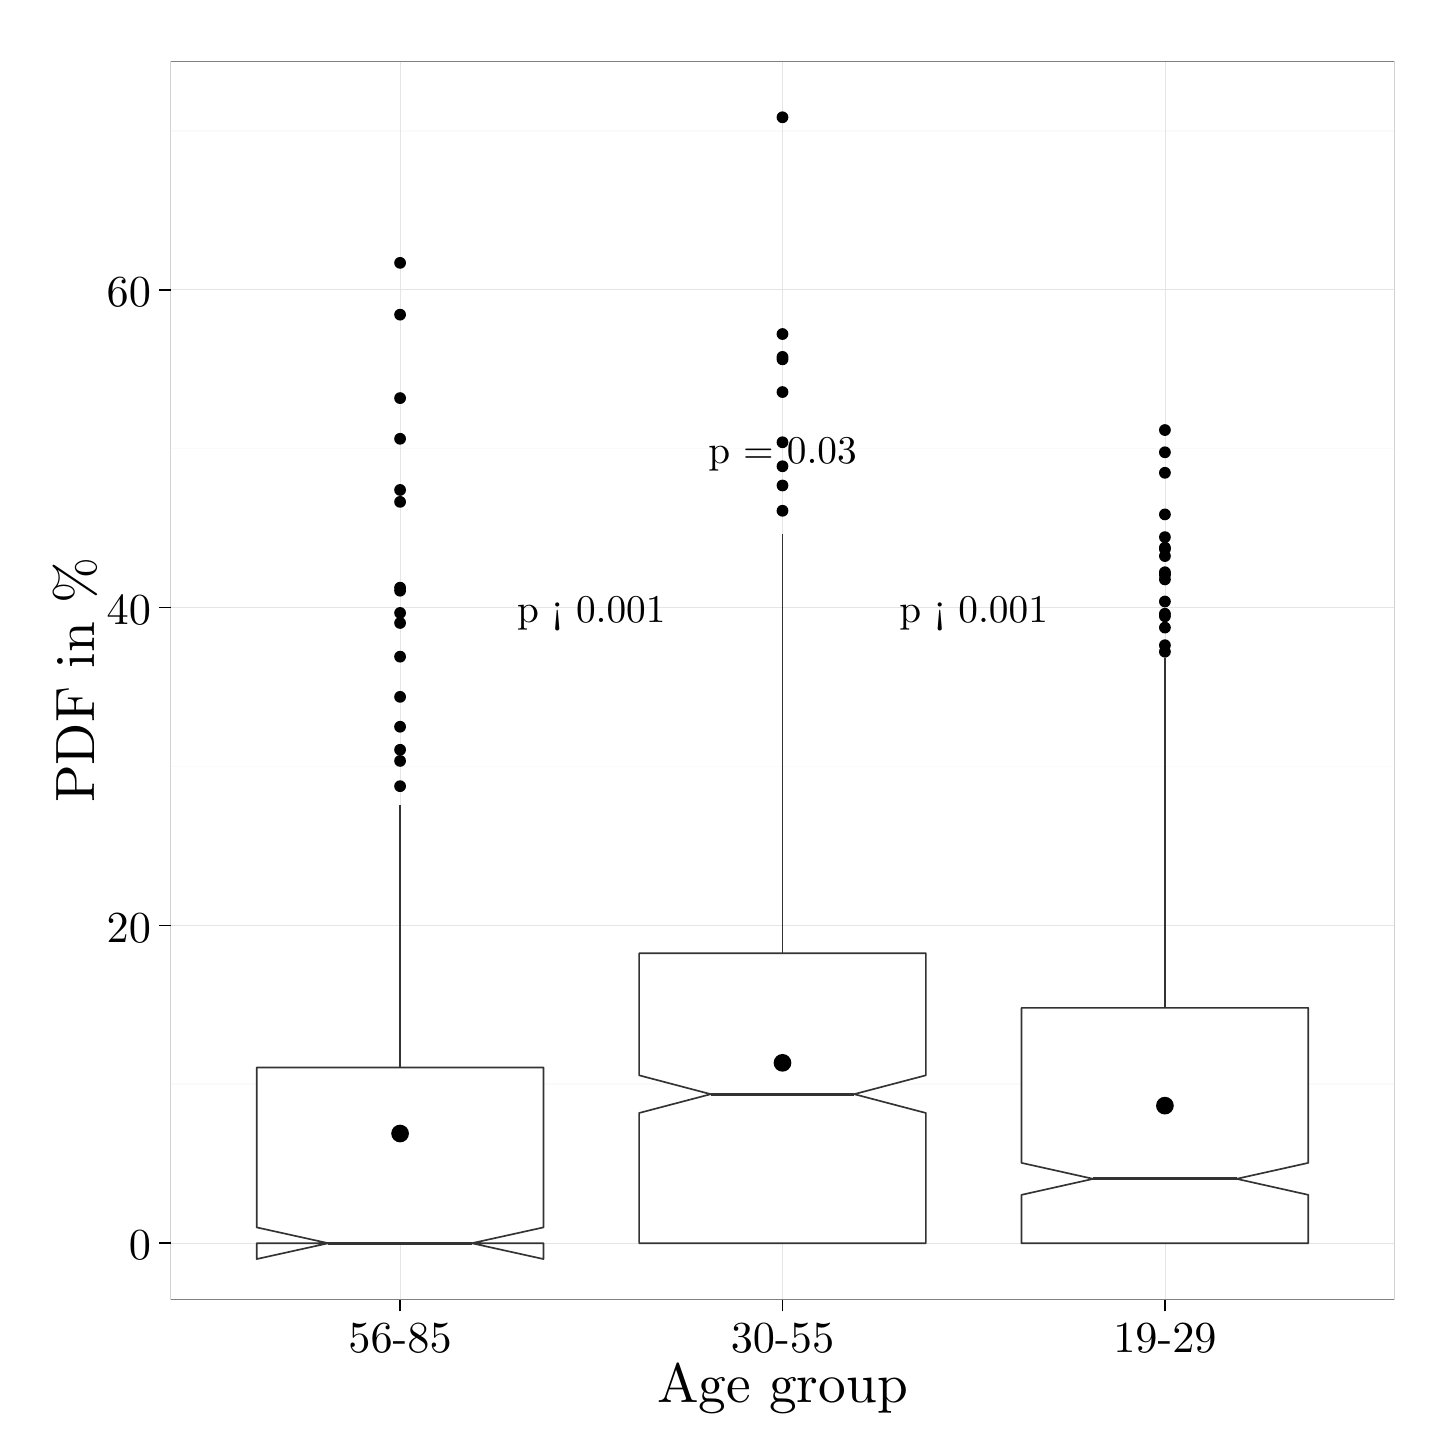
\begin{tikzpicture}[x=1pt,y=1pt]
\definecolor{fillColor}{RGB}{255,255,255}
\path[use as bounding box,fill=fillColor,fill opacity=0.00] (0,0) rectangle (505.89,505.89);
\begin{scope}
\path[clip] (  0.00,  0.00) rectangle (505.89,505.89);
\definecolor{drawColor}{RGB}{255,255,255}
\definecolor{fillColor}{RGB}{255,255,255}

\path[draw=drawColor,line width= 0.6pt,line join=round,line cap=round,fill=fillColor] (  0.00, -0.00) rectangle (505.89,505.89);
\end{scope}
\begin{scope}
\path[clip] ( 51.66, 46.31) rectangle (493.85,493.84);
\definecolor{fillColor}{RGB}{255,255,255}

\path[fill=fillColor] ( 51.66, 46.31) rectangle (493.84,493.84);
\definecolor{drawColor}{gray}{0.98}

\path[draw=drawColor,line width= 0.6pt,line join=round] ( 51.66,124.07) --
	(493.85,124.07);

\path[draw=drawColor,line width= 0.6pt,line join=round] ( 51.66,238.92) --
	(493.85,238.92);

\path[draw=drawColor,line width= 0.6pt,line join=round] ( 51.66,353.77) --
	(493.85,353.77);

\path[draw=drawColor,line width= 0.6pt,line join=round] ( 51.66,468.62) --
	(493.85,468.62);
\definecolor{drawColor}{gray}{0.90}

\path[draw=drawColor,line width= 0.2pt,line join=round] ( 51.66, 66.65) --
	(493.85, 66.65);

\path[draw=drawColor,line width= 0.2pt,line join=round] ( 51.66,181.50) --
	(493.85,181.50);

\path[draw=drawColor,line width= 0.2pt,line join=round] ( 51.66,296.35) --
	(493.85,296.35);

\path[draw=drawColor,line width= 0.2pt,line join=round] ( 51.66,411.20) --
	(493.85,411.20);

\path[draw=drawColor,line width= 0.2pt,line join=round] (134.57, 46.31) --
	(134.57,493.84);

\path[draw=drawColor,line width= 0.2pt,line join=round] (272.75, 46.31) --
	(272.75,493.84);

\path[draw=drawColor,line width= 0.2pt,line join=round] (410.94, 46.31) --
	(410.94,493.84);
\definecolor{fillColor}{RGB}{0,0,0}

\path[fill=fillColor] (134.57,357.33) circle (  2.13);

\path[fill=fillColor] (134.57,290.78) circle (  2.13);

\path[fill=fillColor] (134.57,338.84) circle (  2.13);

\path[fill=fillColor] (134.57,278.60) circle (  2.13);

\path[fill=fillColor] (134.57,231.80) circle (  2.13);

\path[fill=fillColor] (134.57,294.40) circle (  2.13);

\path[fill=fillColor] (134.57,264.08) circle (  2.13);

\path[fill=fillColor] (134.57,334.54) circle (  2.13);

\path[fill=fillColor] (134.57,402.18) circle (  2.13);

\path[fill=fillColor] (134.57,372.03) circle (  2.13);

\path[fill=fillColor] (134.57,303.53) circle (  2.13);

\path[fill=fillColor] (134.57,302.43) circle (  2.13);

\path[fill=fillColor] (134.57,420.90) circle (  2.13);

\path[fill=fillColor] (134.57,240.93) circle (  2.13);

\path[fill=fillColor] (134.57,253.28) circle (  2.13);

\path[fill=fillColor] (134.57,244.95) circle (  2.13);
\definecolor{drawColor}{gray}{0.20}

\path[draw=drawColor,line width= 0.6pt,line join=round] (134.57,130.13) -- (134.57,224.85);

\path[draw=drawColor,line width= 0.6pt,line join=round] (134.57, 66.65) -- (134.57, 66.65);
\definecolor{fillColor}{RGB}{255,255,255}

\path[draw=drawColor,line width= 0.6pt,line join=round,line cap=round,fill=fillColor] ( 82.75,130.13) --
	( 82.75, 72.37) --
	(108.66, 66.65) --
	( 82.75, 60.93) --
	( 82.75, 66.65) --
	(186.39, 66.65) --
	(186.39, 60.93) --
	(160.48, 66.65) --
	(186.39, 72.37) --
	(186.39,130.13) --
	( 82.75,130.13) --
	cycle;

\path[draw=drawColor,line width= 1.1pt,line join=round] (108.66, 66.65) -- (160.48, 66.65);
\definecolor{fillColor}{RGB}{0,0,0}

\path[fill=fillColor] (272.75,395.18) circle (  2.13);

\path[fill=fillColor] (272.75,356.07) circle (  2.13);

\path[fill=fillColor] (272.75,386.91) circle (  2.13);

\path[fill=fillColor] (272.75,347.40) circle (  2.13);

\path[fill=fillColor] (272.75,340.45) circle (  2.13);

\path[fill=fillColor] (272.75,374.22) circle (  2.13);

\path[fill=fillColor] (272.75,473.50) circle (  2.13);

\path[fill=fillColor] (272.75,386.04) circle (  2.13);

\path[fill=fillColor] (272.75,331.32) circle (  2.13);

\path[draw=drawColor,line width= 0.6pt,line join=round] (272.75,171.44) -- (272.75,322.82);

\path[draw=drawColor,line width= 0.6pt,line join=round] (272.75, 66.65) -- (272.75, 66.65);
\definecolor{fillColor}{RGB}{255,255,255}

\path[draw=drawColor,line width= 0.6pt,line join=round,line cap=round,fill=fillColor] (220.94,171.44) --
	(220.94,127.32) --
	(246.84,120.51) --
	(220.94,113.71) --
	(220.94, 66.65) --
	(324.57, 66.65) --
	(324.57,113.71) --
	(298.66,120.51) --
	(324.57,127.32) --
	(324.57,171.44) --
	(220.94,171.44) --
	cycle;

\path[draw=drawColor,line width= 1.1pt,line join=round] (246.84,120.51) -- (298.66,120.51);
\definecolor{fillColor}{RGB}{0,0,0}

\path[fill=fillColor] (410.94,282.74) circle (  2.13);

\path[fill=fillColor] (410.94,294.11) circle (  2.13);

\path[fill=fillColor] (410.94,314.95) circle (  2.13);

\path[fill=fillColor] (410.94,293.19) circle (  2.13);

\path[fill=fillColor] (410.94,309.10) circle (  2.13);

\path[fill=fillColor] (410.94,318.00) circle (  2.13);

\path[fill=fillColor] (410.94,330.00) circle (  2.13);

\path[fill=fillColor] (410.94,345.04) circle (  2.13);

\path[fill=fillColor] (410.94,306.51) circle (  2.13);

\path[fill=fillColor] (410.94,308.69) circle (  2.13);

\path[fill=fillColor] (410.94,289.11) circle (  2.13);

\path[fill=fillColor] (410.94,317.48) circle (  2.13);

\path[fill=fillColor] (410.94,298.53) circle (  2.13);

\path[fill=fillColor] (410.94,280.38) circle (  2.13);

\path[fill=fillColor] (410.94,352.45) circle (  2.13);

\path[fill=fillColor] (410.94,308.12) circle (  2.13);

\path[fill=fillColor] (410.94,360.49) circle (  2.13);

\path[fill=fillColor] (410.94,321.79) circle (  2.13);

\path[draw=drawColor,line width= 0.6pt,line join=round] (410.94,151.70) -- (410.94,278.26);

\path[draw=drawColor,line width= 0.6pt,line join=round] (410.94, 66.65) -- (410.94, 66.65);
\definecolor{fillColor}{RGB}{255,255,255}

\path[draw=drawColor,line width= 0.6pt,line join=round,line cap=round,fill=fillColor] (359.12,151.70) --
	(359.12, 95.68) --
	(385.03, 89.91) --
	(359.12, 84.13) --
	(359.12, 66.65) --
	(462.75, 66.65) --
	(462.75, 84.13) --
	(436.84, 89.91) --
	(462.75, 95.68) --
	(462.75,151.70) --
	(359.12,151.70) --
	cycle;

\path[draw=drawColor,line width= 1.1pt,line join=round] (385.03, 89.91) -- (436.84, 89.91);
\definecolor{fillColor}{RGB}{0,0,0}

\path[fill=fillColor] (134.57,106.29) circle (  3.20);

\path[fill=fillColor] (272.75,131.83) circle (  3.20);

\path[fill=fillColor] (410.94,116.36) circle (  3.20);
\definecolor{drawColor}{RGB}{0,0,0}

\node[text=drawColor,anchor=base,inner sep=0pt, outer sep=0pt, scale=  1.42] at (203.66,291.00) {p < 0.001};

\node[text=drawColor,anchor=base,inner sep=0pt, outer sep=0pt, scale=  1.42] at (341.84,291.00) {p < 0.001};

\node[text=drawColor,anchor=base,inner sep=0pt, outer sep=0pt, scale=  1.42] at (272.75,348.43) {p = 0.03};
\definecolor{drawColor}{gray}{0.50}

\path[draw=drawColor,line width= 0.6pt,line join=round,line cap=round] ( 51.66, 46.31) rectangle (493.84,493.84);
\end{scope}
\begin{scope}
\path[clip] (  0.00,  0.00) rectangle (505.89,505.89);
\definecolor{drawColor}{RGB}{0,0,0}

\node[text=drawColor,anchor=base east,inner sep=0pt, outer sep=0pt, scale=  1.60] at ( 44.55, 60.62) {0};

\node[text=drawColor,anchor=base east,inner sep=0pt, outer sep=0pt, scale=  1.60] at ( 44.55,175.47) {20};

\node[text=drawColor,anchor=base east,inner sep=0pt, outer sep=0pt, scale=  1.60] at ( 44.55,290.31) {40};

\node[text=drawColor,anchor=base east,inner sep=0pt, outer sep=0pt, scale=  1.60] at ( 44.55,405.16) {60};
\end{scope}
\begin{scope}
\path[clip] (  0.00,  0.00) rectangle (505.89,505.89);
\definecolor{drawColor}{RGB}{0,0,0}

\path[draw=drawColor,line width= 0.6pt,line join=round] ( 47.39, 66.65) --
	( 51.66, 66.65);

\path[draw=drawColor,line width= 0.6pt,line join=round] ( 47.39,181.50) --
	( 51.66,181.50);

\path[draw=drawColor,line width= 0.6pt,line join=round] ( 47.39,296.35) --
	( 51.66,296.35);

\path[draw=drawColor,line width= 0.6pt,line join=round] ( 47.39,411.20) --
	( 51.66,411.20);
\end{scope}
\begin{scope}
\path[clip] (  0.00,  0.00) rectangle (505.89,505.89);
\definecolor{drawColor}{RGB}{0,0,0}

\path[draw=drawColor,line width= 0.6pt,line join=round] (134.57, 42.04) --
	(134.57, 46.31);

\path[draw=drawColor,line width= 0.6pt,line join=round] (272.75, 42.04) --
	(272.75, 46.31);

\path[draw=drawColor,line width= 0.6pt,line join=round] (410.94, 42.04) --
	(410.94, 46.31);
\end{scope}
\begin{scope}
\path[clip] (  0.00,  0.00) rectangle (505.89,505.89);
\definecolor{drawColor}{RGB}{0,0,0}

\node[text=drawColor,anchor=base,inner sep=0pt, outer sep=0pt, scale=  1.60] at (134.57, 27.13) {56-85};

\node[text=drawColor,anchor=base,inner sep=0pt, outer sep=0pt, scale=  1.60] at (272.75, 27.13) {30-55};

\node[text=drawColor,anchor=base,inner sep=0pt, outer sep=0pt, scale=  1.60] at (410.94, 27.13) {19-29};
\end{scope}
\begin{scope}
\path[clip] (  0.00,  0.00) rectangle (505.89,505.89);
\definecolor{drawColor}{RGB}{0,0,0}

\node[text=drawColor,anchor=base,inner sep=0pt, outer sep=0pt, scale=  2.00] at (272.75,  9.03) {Age group};
\end{scope}
\begin{scope}
\path[clip] (  0.00,  0.00) rectangle (505.89,505.89);
\definecolor{drawColor}{RGB}{0,0,0}

\node[text=drawColor,rotate= 90.00,anchor=base,inner sep=0pt, outer sep=0pt, scale=  2.00] at ( 24.12,270.08) {PDF in {\%}};
\end{scope}
\end{tikzpicture}
} 
	\caption{/ŋ(g)/: PDF by age ([ɪn] excluded)}
	\label{fig.box.ng.tot}
\end{figure}

Before the second interaction retained in the mixed-effects model (age X social class) is analysed further, we will have a brief look at age of participant as a main effect (\figref{fig.box.ng.tot}).
The relatively high number of outliers in all groups shows that at least occasionally all speakers use variants of /ŋ(g)/ that contain a (prominent) plosive and are thus clearly Scouse.
The overall rather low figures (the upper boundaries of all boxes are below 20\%) are not really surprising, given the fact that even if a plosive is realised it is preceded by a nasal, so the aspiration phase will almost always be comparatively short in relation to the total duration.
It is furthermore obvious that things are not the way we expected.
The oldest speakers are the least Scouse with respect to velar nasal plus.
Their average \isi{PDF} is only 6.9\%, while that of the middle group is, at 11.35\%, almost twice as high.
Furthermore, the median in the former group (again symbolised by the thick horizontal bar) is 0, so 50+\% of all their /ŋ(g)/ realisations consist of a nasal only.
For the middle-aged speakers, on the other hand, the median is found at a \isi{PDF} of around 10\% and only the first quantile is 0, so somewhere between 50 and 75\% of tokens have a plosive.
The increase in \isi{PDF} from the oldest to the middle-aged speakers is highly significant (t(663.417) = 5.437, p < 0.001).
From the middle to the young group, however, there is actually a \emph{de}crease in \isi{PDF} to 8.66\%.
This means that younger Liverpudlians are not getting ``more Scouse'' with respect to velar nasal plus, but rather they seem to be reversing the trend begun by the middle group of speakers, although not to the extent that their realisations are identical to those of their grandparents' generation.
Rather, they occupy the middle ground, since both their mean and median are higher than in the older and lower than in the middle group.
The youngest speakers in the sample use velar nasal plus in a significantly different way from both the old (t(630.154) = 2.178, p = 0.03), \emph{and} the middle-aged group (t(1130.999) = -3.881, p < 0.001).

\begin{figure}[h]
	\centering
	\begin{subfigure}{.49\textwidth}
		\centering
			\definecolor{shadecolor}{rgb}{0.969, 0.969, 0.969}
			\resizebox{\linewidth}{!}{% Created by tikzDevice version 0.8.1 on 2016-02-09 02:16:55
% !TEX encoding = UTF-8 Unicode
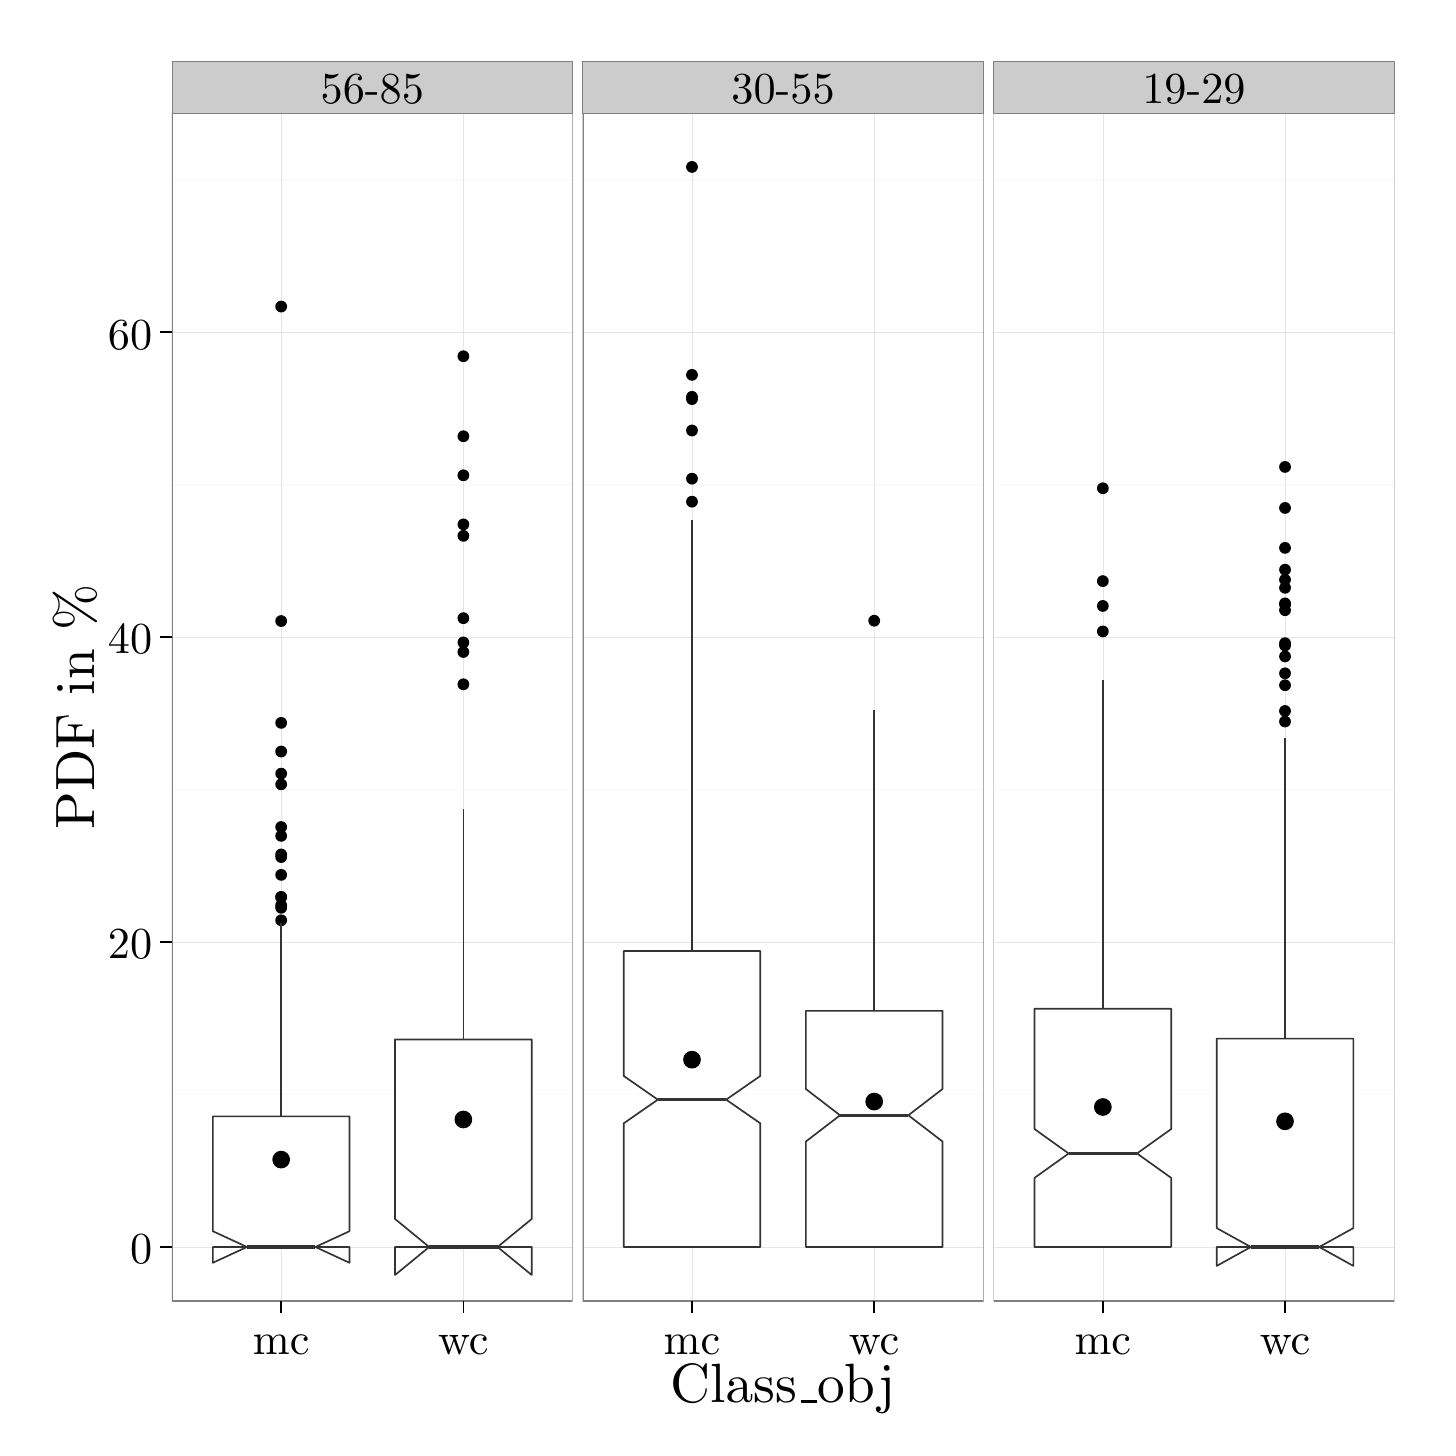
\begin{tikzpicture}[x=1pt,y=1pt]
\definecolor{fillColor}{RGB}{255,255,255}
\path[use as bounding box,fill=fillColor,fill opacity=0.00] (0,0) rectangle (505.89,505.89);
\begin{scope}
\path[clip] (  0.00,  0.00) rectangle (505.89,505.89);
\definecolor{drawColor}{RGB}{255,255,255}
\definecolor{fillColor}{RGB}{255,255,255}

\path[draw=drawColor,line width= 0.6pt,line join=round,line cap=round,fill=fillColor] (  0.00, -0.00) rectangle (505.89,505.89);
\end{scope}
\begin{scope}
\path[clip] ( 52.10, 45.77) rectangle (196.94,475.09);
\definecolor{fillColor}{RGB}{255,255,255}

\path[fill=fillColor] ( 52.10, 45.77) rectangle (196.94,475.09);
\definecolor{drawColor}{gray}{0.98}

\path[draw=drawColor,line width= 0.6pt,line join=round] ( 52.10,120.37) --
	(196.94,120.37);

\path[draw=drawColor,line width= 0.6pt,line join=round] ( 52.10,230.55) --
	(196.94,230.55);

\path[draw=drawColor,line width= 0.6pt,line join=round] ( 52.10,340.72) --
	(196.94,340.72);

\path[draw=drawColor,line width= 0.6pt,line join=round] ( 52.10,450.89) --
	(196.94,450.89);
\definecolor{drawColor}{gray}{0.90}

\path[draw=drawColor,line width= 0.2pt,line join=round] ( 52.10, 65.29) --
	(196.94, 65.29);

\path[draw=drawColor,line width= 0.2pt,line join=round] ( 52.10,175.46) --
	(196.94,175.46);

\path[draw=drawColor,line width= 0.2pt,line join=round] ( 52.10,285.63) --
	(196.94,285.63);

\path[draw=drawColor,line width= 0.2pt,line join=round] ( 52.10,395.80) --
	(196.94,395.80);

\path[draw=drawColor,line width= 0.2pt,line join=round] ( 91.60, 45.77) --
	( 91.60,475.09);

\path[draw=drawColor,line width= 0.2pt,line join=round] (157.44, 45.77) --
	(157.44,475.09);
\definecolor{fillColor}{RGB}{0,0,0}

\path[fill=fillColor] ( 91.60,254.67) circle (  2.13);

\path[fill=fillColor] ( 91.60,191.71) circle (  2.13);

\path[fill=fillColor] ( 91.60,191.76) circle (  2.13);

\path[fill=fillColor] ( 91.60,291.47) circle (  2.13);

\path[fill=fillColor] ( 91.60,187.85) circle (  2.13);

\path[fill=fillColor] ( 91.60,405.11) circle (  2.13);

\path[fill=fillColor] ( 91.60,213.85) circle (  2.13);

\path[fill=fillColor] ( 91.60,232.47) circle (  2.13);

\path[fill=fillColor] ( 91.60,207.13) circle (  2.13);

\path[fill=fillColor] ( 91.60,244.32) circle (  2.13);

\path[fill=fillColor] ( 91.60,188.79) circle (  2.13);

\path[fill=fillColor] ( 91.60,217.05) circle (  2.13);

\path[fill=fillColor] ( 91.60,236.33) circle (  2.13);

\path[fill=fillColor] ( 91.60,206.20) circle (  2.13);

\path[fill=fillColor] ( 91.60,199.75) circle (  2.13);

\path[fill=fillColor] ( 91.60,183.34) circle (  2.13);
\definecolor{drawColor}{gray}{0.20}

\path[draw=drawColor,line width= 0.6pt,line join=round] ( 91.60,112.50) -- ( 91.60,182.45);

\path[draw=drawColor,line width= 0.6pt,line join=round] ( 91.60, 65.29) -- ( 91.60, 65.29);
\definecolor{fillColor}{RGB}{255,255,255}

\path[draw=drawColor,line width= 0.6pt,line join=round,line cap=round,fill=fillColor] ( 66.91,112.50) --
	( 66.91, 70.99) --
	( 79.26, 65.29) --
	( 66.91, 59.58) --
	( 66.91, 65.29) --
	(116.29, 65.29) --
	(116.29, 59.58) --
	(103.95, 65.29) --
	(116.29, 70.99) --
	(116.29,112.50) --
	( 66.91,112.50) --
	cycle;

\path[draw=drawColor,line width= 1.1pt,line join=round] ( 79.26, 65.29) -- (103.95, 65.29);
\definecolor{fillColor}{RGB}{0,0,0}

\path[fill=fillColor] (157.44,344.13) circle (  2.13);

\path[fill=fillColor] (157.44,280.29) circle (  2.13);

\path[fill=fillColor] (157.44,326.40) circle (  2.13);

\path[fill=fillColor] (157.44,268.61) circle (  2.13);

\path[fill=fillColor] (157.44,283.76) circle (  2.13);

\path[fill=fillColor] (157.44,322.26) circle (  2.13);

\path[fill=fillColor] (157.44,387.16) circle (  2.13);

\path[fill=fillColor] (157.44,358.24) circle (  2.13);

\path[fill=fillColor] (157.44,292.52) circle (  2.13);

\path[draw=drawColor,line width= 0.6pt,line join=round] (157.44,140.26) -- (157.44,223.71);

\path[draw=drawColor,line width= 0.6pt,line join=round] (157.44, 65.29) -- (157.44, 65.29);
\definecolor{fillColor}{RGB}{255,255,255}

\path[draw=drawColor,line width= 0.6pt,line join=round,line cap=round,fill=fillColor] (132.75,140.26) --
	(132.75, 75.41) --
	(145.09, 65.29) --
	(132.75, 55.17) --
	(132.75, 65.29) --
	(182.13, 65.29) --
	(182.13, 55.17) --
	(169.78, 65.29) --
	(182.13, 75.41) --
	(182.13,140.26) --
	(132.75,140.26) --
	cycle;

\path[draw=drawColor,line width= 1.1pt,line join=round] (145.09, 65.29) -- (169.78, 65.29);
\definecolor{fillColor}{RGB}{0,0,0}

\path[fill=fillColor] ( 91.60, 96.87) circle (  3.20);

\path[fill=fillColor] (157.44,111.36) circle (  3.20);
\definecolor{drawColor}{gray}{0.50}

\path[draw=drawColor,line width= 0.6pt,line join=round,line cap=round] ( 52.10, 45.77) rectangle (196.94,475.09);
\end{scope}
\begin{scope}
\path[clip] (200.55, 45.77) rectangle (345.39,475.09);
\definecolor{fillColor}{RGB}{255,255,255}

\path[fill=fillColor] (200.55, 45.77) rectangle (345.39,475.09);
\definecolor{drawColor}{gray}{0.98}

\path[draw=drawColor,line width= 0.6pt,line join=round] (200.55,120.37) --
	(345.39,120.37);

\path[draw=drawColor,line width= 0.6pt,line join=round] (200.55,230.55) --
	(345.39,230.55);

\path[draw=drawColor,line width= 0.6pt,line join=round] (200.55,340.72) --
	(345.39,340.72);

\path[draw=drawColor,line width= 0.6pt,line join=round] (200.55,450.89) --
	(345.39,450.89);
\definecolor{drawColor}{gray}{0.90}

\path[draw=drawColor,line width= 0.2pt,line join=round] (200.55, 65.29) --
	(345.39, 65.29);

\path[draw=drawColor,line width= 0.2pt,line join=round] (200.55,175.46) --
	(345.39,175.46);

\path[draw=drawColor,line width= 0.2pt,line join=round] (200.55,285.63) --
	(345.39,285.63);

\path[draw=drawColor,line width= 0.2pt,line join=round] (200.55,395.80) --
	(345.39,395.80);

\path[draw=drawColor,line width= 0.2pt,line join=round] (240.05, 45.77) --
	(240.05,475.09);

\path[draw=drawColor,line width= 0.2pt,line join=round] (305.89, 45.77) --
	(305.89,475.09);
\definecolor{fillColor}{RGB}{0,0,0}

\path[fill=fillColor] (240.05,380.43) circle (  2.13);

\path[fill=fillColor] (240.05,342.92) circle (  2.13);

\path[fill=fillColor] (240.05,372.50) circle (  2.13);

\path[fill=fillColor] (240.05,334.60) circle (  2.13);

\path[fill=fillColor] (240.05,360.33) circle (  2.13);

\path[fill=fillColor] (240.05,455.57) circle (  2.13);

\path[fill=fillColor] (240.05,371.68) circle (  2.13);
\definecolor{drawColor}{gray}{0.20}

\path[draw=drawColor,line width= 0.6pt,line join=round] (240.05,172.25) -- (240.05,327.94);

\path[draw=drawColor,line width= 0.6pt,line join=round] (240.05, 65.29) -- (240.05, 65.29);
\definecolor{fillColor}{RGB}{255,255,255}

\path[draw=drawColor,line width= 0.6pt,line join=round,line cap=round,fill=fillColor] (215.37,172.25) --
	(215.37,127.09) --
	(227.71,118.53) --
	(215.37,109.97) --
	(215.37, 65.29) --
	(264.74, 65.29) --
	(264.74,109.97) --
	(252.40,118.53) --
	(264.74,127.09) --
	(264.74,172.25) --
	(215.37,172.25) --
	cycle;

\path[draw=drawColor,line width= 1.1pt,line join=round] (227.71,118.53) -- (252.40,118.53);
\definecolor{fillColor}{RGB}{0,0,0}

\path[fill=fillColor] (305.89,291.58) circle (  2.13);

\path[draw=drawColor,line width= 0.6pt,line join=round] (305.89,150.62) -- (305.89,259.36);

\path[draw=drawColor,line width= 0.6pt,line join=round] (305.89, 65.29) -- (305.89, 65.29);
\definecolor{fillColor}{RGB}{255,255,255}

\path[draw=drawColor,line width= 0.6pt,line join=round,line cap=round,fill=fillColor] (281.20,150.62) --
	(281.20,122.37) --
	(293.55,112.88) --
	(281.20,103.40) --
	(281.20, 65.29) --
	(330.58, 65.29) --
	(330.58,103.40) --
	(318.23,112.88) --
	(330.58,122.37) --
	(330.58,150.62) --
	(281.20,150.62) --
	cycle;

\path[draw=drawColor,line width= 1.1pt,line join=round] (293.55,112.88) -- (318.23,112.88);
\definecolor{fillColor}{RGB}{0,0,0}

\path[fill=fillColor] (240.05,132.98) circle (  3.20);

\path[fill=fillColor] (305.89,117.84) circle (  3.20);
\definecolor{drawColor}{gray}{0.50}

\path[draw=drawColor,line width= 0.6pt,line join=round,line cap=round] (200.55, 45.77) rectangle (345.39,475.09);
\end{scope}
\begin{scope}
\path[clip] (349.01, 45.77) rectangle (493.85,475.09);
\definecolor{fillColor}{RGB}{255,255,255}

\path[fill=fillColor] (349.01, 45.77) rectangle (493.85,475.09);
\definecolor{drawColor}{gray}{0.98}

\path[draw=drawColor,line width= 0.6pt,line join=round] (349.01,120.37) --
	(493.85,120.37);

\path[draw=drawColor,line width= 0.6pt,line join=round] (349.01,230.55) --
	(493.85,230.55);

\path[draw=drawColor,line width= 0.6pt,line join=round] (349.01,340.72) --
	(493.85,340.72);

\path[draw=drawColor,line width= 0.6pt,line join=round] (349.01,450.89) --
	(493.85,450.89);
\definecolor{drawColor}{gray}{0.90}

\path[draw=drawColor,line width= 0.2pt,line join=round] (349.01, 65.29) --
	(493.85, 65.29);

\path[draw=drawColor,line width= 0.2pt,line join=round] (349.01,175.46) --
	(493.85,175.46);

\path[draw=drawColor,line width= 0.2pt,line join=round] (349.01,285.63) --
	(493.85,285.63);

\path[draw=drawColor,line width= 0.2pt,line join=round] (349.01,395.80) --
	(493.85,395.80);

\path[draw=drawColor,line width= 0.2pt,line join=round] (388.51, 45.77) --
	(388.51,475.09);

\path[draw=drawColor,line width= 0.2pt,line join=round] (454.34, 45.77) --
	(454.34,475.09);
\definecolor{fillColor}{RGB}{0,0,0}

\path[fill=fillColor] (388.51,305.90) circle (  2.13);

\path[fill=fillColor] (388.51,287.72) circle (  2.13);

\path[fill=fillColor] (388.51,339.45) circle (  2.13);

\path[fill=fillColor] (388.51,296.92) circle (  2.13);
\definecolor{drawColor}{gray}{0.20}

\path[draw=drawColor,line width= 0.6pt,line join=round] (388.51,151.40) -- (388.51,270.32);

\path[draw=drawColor,line width= 0.6pt,line join=round] (388.51, 65.29) -- (388.51, 65.29);
\definecolor{fillColor}{RGB}{255,255,255}

\path[draw=drawColor,line width= 0.6pt,line join=round,line cap=round,fill=fillColor] (363.82,151.40) --
	(363.82,107.90) --
	(376.16, 99.08) --
	(363.82, 90.26) --
	(363.82, 65.29) --
	(413.20, 65.29) --
	(413.20, 90.26) --
	(400.85, 99.08) --
	(413.20,107.90) --
	(413.20,151.40) --
	(363.82,151.40) --
	cycle;

\path[draw=drawColor,line width= 1.1pt,line join=round] (376.16, 99.08) -- (400.85, 99.08);
\definecolor{fillColor}{RGB}{0,0,0}

\path[fill=fillColor] (454.34,272.58) circle (  2.13);

\path[fill=fillColor] (454.34,283.48) circle (  2.13);

\path[fill=fillColor] (454.34,303.48) circle (  2.13);

\path[fill=fillColor] (454.34,282.60) circle (  2.13);

\path[fill=fillColor] (454.34,297.86) circle (  2.13);

\path[fill=fillColor] (454.34,306.40) circle (  2.13);

\path[fill=fillColor] (454.34,317.91) circle (  2.13);

\path[fill=fillColor] (454.34,268.28) circle (  2.13);

\path[fill=fillColor] (454.34,332.34) circle (  2.13);

\path[fill=fillColor] (454.34,295.38) circle (  2.13);

\path[fill=fillColor] (454.34,297.48) circle (  2.13);

\path[fill=fillColor] (454.34,278.69) circle (  2.13);

\path[fill=fillColor] (454.34,347.16) circle (  2.13);

\path[fill=fillColor] (454.34,310.03) circle (  2.13);

\path[fill=fillColor] (454.34,255.17) circle (  2.13);

\path[fill=fillColor] (454.34,258.97) circle (  2.13);

\path[draw=drawColor,line width= 0.6pt,line join=round] (454.34,140.59) -- (454.34,249.05);

\path[draw=drawColor,line width= 0.6pt,line join=round] (454.34, 65.29) -- (454.34, 65.29);
\definecolor{fillColor}{RGB}{255,255,255}

\path[draw=drawColor,line width= 0.6pt,line join=round,line cap=round,fill=fillColor] (429.65,140.59) --
	(429.65, 72.12) --
	(442.00, 65.29) --
	(429.65, 58.45) --
	(429.65, 65.29) --
	(479.03, 65.29) --
	(479.03, 58.45) --
	(466.69, 65.29) --
	(479.03, 72.12) --
	(479.03,140.59) --
	(429.65,140.59) --
	cycle;

\path[draw=drawColor,line width= 1.1pt,line join=round] (442.00, 65.29) -- (466.69, 65.29);
\definecolor{fillColor}{RGB}{0,0,0}

\path[fill=fillColor] (388.51,115.87) circle (  3.20);

\path[fill=fillColor] (454.34,110.70) circle (  3.20);
\definecolor{drawColor}{gray}{0.50}

\path[draw=drawColor,line width= 0.6pt,line join=round,line cap=round] (349.01, 45.77) rectangle (493.85,475.09);
\end{scope}
\begin{scope}
\path[clip] (  0.00,  0.00) rectangle (505.89,505.89);
\definecolor{drawColor}{gray}{0.50}
\definecolor{fillColor}{gray}{0.80}

\path[draw=drawColor,line width= 0.2pt,line join=round,line cap=round,fill=fillColor] ( 52.10,475.09) rectangle (196.94,493.85);
\definecolor{drawColor}{RGB}{0,0,0}

\node[text=drawColor,anchor=base,inner sep=0pt, outer sep=0pt, scale=  1.60] at (124.52,478.43) {56-85};
\end{scope}
\begin{scope}
\path[clip] (  0.00,  0.00) rectangle (505.89,505.89);
\definecolor{drawColor}{gray}{0.50}
\definecolor{fillColor}{gray}{0.80}

\path[draw=drawColor,line width= 0.2pt,line join=round,line cap=round,fill=fillColor] (200.55,475.09) rectangle (345.39,493.85);
\definecolor{drawColor}{RGB}{0,0,0}

\node[text=drawColor,anchor=base,inner sep=0pt, outer sep=0pt, scale=  1.60] at (272.97,478.43) {30-55};
\end{scope}
\begin{scope}
\path[clip] (  0.00,  0.00) rectangle (505.89,505.89);
\definecolor{drawColor}{gray}{0.50}
\definecolor{fillColor}{gray}{0.80}

\path[draw=drawColor,line width= 0.2pt,line join=round,line cap=round,fill=fillColor] (349.01,475.09) rectangle (493.85,493.85);
\definecolor{drawColor}{RGB}{0,0,0}

\node[text=drawColor,anchor=base,inner sep=0pt, outer sep=0pt, scale=  1.60] at (421.43,478.43) {19-29};
\end{scope}
\begin{scope}
\path[clip] (  0.00,  0.00) rectangle (505.89,505.89);
\definecolor{drawColor}{RGB}{0,0,0}

\node[text=drawColor,anchor=base east,inner sep=0pt, outer sep=0pt, scale=  1.60] at ( 44.99, 59.25) {0};

\node[text=drawColor,anchor=base east,inner sep=0pt, outer sep=0pt, scale=  1.60] at ( 44.99,169.43) {20};

\node[text=drawColor,anchor=base east,inner sep=0pt, outer sep=0pt, scale=  1.60] at ( 44.99,279.60) {40};

\node[text=drawColor,anchor=base east,inner sep=0pt, outer sep=0pt, scale=  1.60] at ( 44.99,389.77) {60};
\end{scope}
\begin{scope}
\path[clip] (  0.00,  0.00) rectangle (505.89,505.89);
\definecolor{drawColor}{RGB}{0,0,0}

\path[draw=drawColor,line width= 0.6pt,line join=round] ( 47.83, 65.29) --
	( 52.10, 65.29);

\path[draw=drawColor,line width= 0.6pt,line join=round] ( 47.83,175.46) --
	( 52.10,175.46);

\path[draw=drawColor,line width= 0.6pt,line join=round] ( 47.83,285.63) --
	( 52.10,285.63);

\path[draw=drawColor,line width= 0.6pt,line join=round] ( 47.83,395.80) --
	( 52.10,395.80);
\end{scope}
\begin{scope}
\path[clip] (  0.00,  0.00) rectangle (505.89,505.89);
\definecolor{drawColor}{RGB}{0,0,0}

\path[draw=drawColor,line width= 0.6pt,line join=round] ( 91.60, 41.50) --
	( 91.60, 45.77);

\path[draw=drawColor,line width= 0.6pt,line join=round] (157.44, 41.50) --
	(157.44, 45.77);
\end{scope}
\begin{scope}
\path[clip] (  0.00,  0.00) rectangle (505.89,505.89);
\definecolor{drawColor}{RGB}{0,0,0}

\node[text=drawColor,anchor=base,inner sep=0pt, outer sep=0pt, scale=  1.60] at ( 91.60, 26.59) {mc};

\node[text=drawColor,anchor=base,inner sep=0pt, outer sep=0pt, scale=  1.60] at (157.44, 26.59) {wc};
\end{scope}
\begin{scope}
\path[clip] (  0.00,  0.00) rectangle (505.89,505.89);
\definecolor{drawColor}{RGB}{0,0,0}

\path[draw=drawColor,line width= 0.6pt,line join=round] (240.05, 41.50) --
	(240.05, 45.77);

\path[draw=drawColor,line width= 0.6pt,line join=round] (305.89, 41.50) --
	(305.89, 45.77);
\end{scope}
\begin{scope}
\path[clip] (  0.00,  0.00) rectangle (505.89,505.89);
\definecolor{drawColor}{RGB}{0,0,0}

\node[text=drawColor,anchor=base,inner sep=0pt, outer sep=0pt, scale=  1.60] at (240.05, 26.59) {mc};

\node[text=drawColor,anchor=base,inner sep=0pt, outer sep=0pt, scale=  1.60] at (305.89, 26.59) {wc};
\end{scope}
\begin{scope}
\path[clip] (  0.00,  0.00) rectangle (505.89,505.89);
\definecolor{drawColor}{RGB}{0,0,0}

\path[draw=drawColor,line width= 0.6pt,line join=round] (388.51, 41.50) --
	(388.51, 45.77);

\path[draw=drawColor,line width= 0.6pt,line join=round] (454.34, 41.50) --
	(454.34, 45.77);
\end{scope}
\begin{scope}
\path[clip] (  0.00,  0.00) rectangle (505.89,505.89);
\definecolor{drawColor}{RGB}{0,0,0}

\node[text=drawColor,anchor=base,inner sep=0pt, outer sep=0pt, scale=  1.60] at (388.51, 26.59) {mc};

\node[text=drawColor,anchor=base,inner sep=0pt, outer sep=0pt, scale=  1.60] at (454.34, 26.59) {wc};
\end{scope}
\begin{scope}
\path[clip] (  0.00,  0.00) rectangle (505.89,505.89);
\definecolor{drawColor}{RGB}{0,0,0}

\node[text=drawColor,anchor=base,inner sep=0pt, outer sep=0pt, scale=  2.00] at (272.97,  9.03) {Class{\_{}}obj};
\end{scope}
\begin{scope}
\path[clip] (  0.00,  0.00) rectangle (505.89,505.89);
\definecolor{drawColor}{RGB}{0,0,0}

\node[text=drawColor,rotate= 90.00,anchor=base,inner sep=0pt, outer sep=0pt, scale=  2.00] at ( 24.12,260.43) {PDF in {\%}};
\end{scope}
\end{tikzpicture}
} 
		\caption{box plot}
		\label{fig.box.ng.ageclass}
	\end{subfigure}
	\begin{subfigure}{.49\textwidth}
		\centering
			\definecolor{shadecolor}{rgb}{0.969, 0.969, 0.969}
			\resizebox{\linewidth}{!}{% Created by tikzDevice version 0.8.1 on 2016-02-09 02:16:58
% !TEX encoding = UTF-8 Unicode
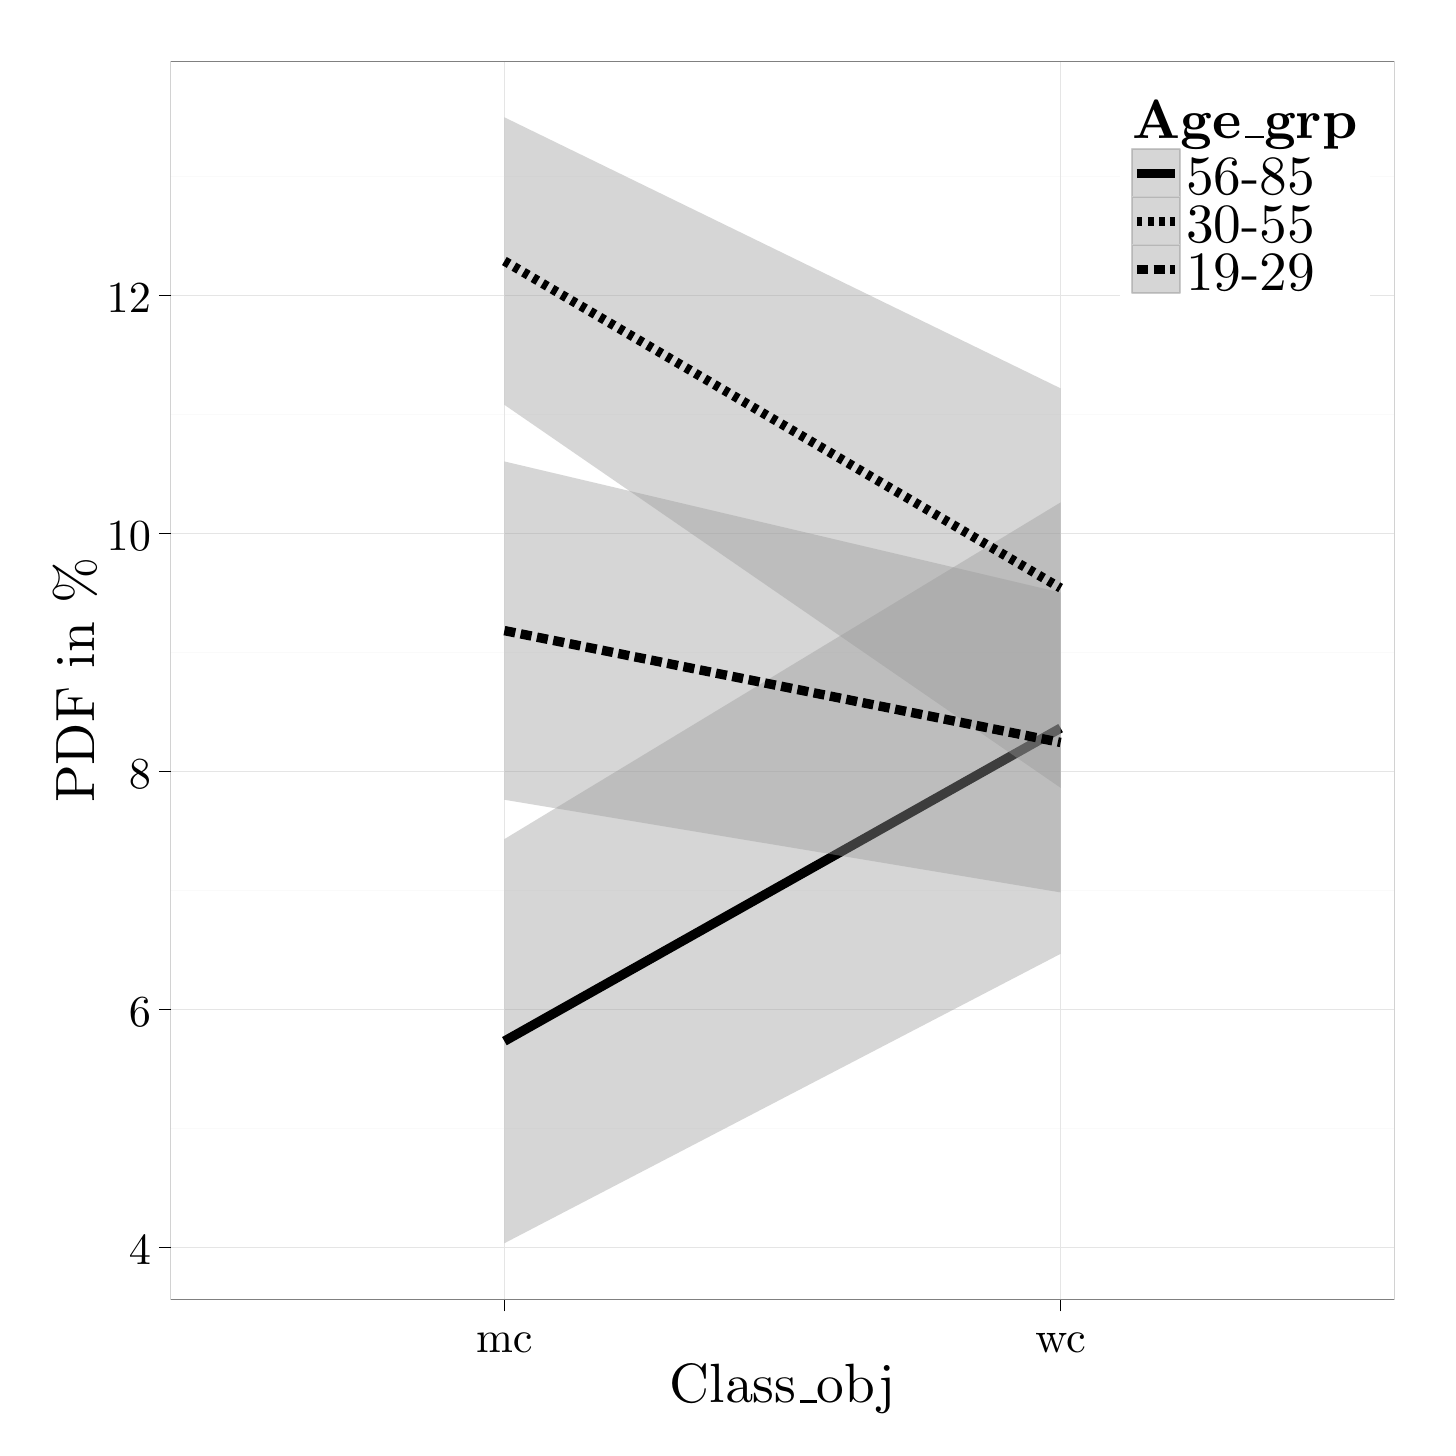
\begin{tikzpicture}[x=1pt,y=1pt]
\definecolor{fillColor}{RGB}{255,255,255}
\path[use as bounding box,fill=fillColor,fill opacity=0.00] (0,0) rectangle (505.89,505.89);
\begin{scope}
\path[clip] (  0.00,  0.00) rectangle (505.89,505.89);
\definecolor{drawColor}{RGB}{255,255,255}
\definecolor{fillColor}{RGB}{255,255,255}

\path[draw=drawColor,line width= 0.6pt,line join=round,line cap=round,fill=fillColor] (  0.00, -0.00) rectangle (505.89,505.89);
\end{scope}
\begin{scope}
\path[clip] ( 51.66, 46.31) rectangle (493.85,493.84);
\definecolor{fillColor}{RGB}{255,255,255}

\path[fill=fillColor] ( 51.66, 46.31) rectangle (493.84,493.84);
\definecolor{drawColor}{gray}{0.98}

\path[draw=drawColor,line width= 0.6pt,line join=round] ( 51.66,108.12) --
	(493.85,108.12);

\path[draw=drawColor,line width= 0.6pt,line join=round] ( 51.66,194.13) --
	(493.85,194.13);

\path[draw=drawColor,line width= 0.6pt,line join=round] ( 51.66,280.13) --
	(493.85,280.13);

\path[draw=drawColor,line width= 0.6pt,line join=round] ( 51.66,366.13) --
	(493.85,366.13);

\path[draw=drawColor,line width= 0.6pt,line join=round] ( 51.66,452.13) --
	(493.85,452.13);
\definecolor{drawColor}{gray}{0.90}

\path[draw=drawColor,line width= 0.2pt,line join=round] ( 51.66, 65.12) --
	(493.85, 65.12);

\path[draw=drawColor,line width= 0.2pt,line join=round] ( 51.66,151.12) --
	(493.85,151.12);

\path[draw=drawColor,line width= 0.2pt,line join=round] ( 51.66,237.13) --
	(493.85,237.13);

\path[draw=drawColor,line width= 0.2pt,line join=round] ( 51.66,323.13) --
	(493.85,323.13);

\path[draw=drawColor,line width= 0.2pt,line join=round] ( 51.66,409.13) --
	(493.85,409.13);

\path[draw=drawColor,line width= 0.2pt,line join=round] (172.26, 46.31) --
	(172.26,493.84);

\path[draw=drawColor,line width= 0.2pt,line join=round] (373.25, 46.31) --
	(373.25,493.84);
\definecolor{fillColor}{RGB}{153,153,153}

\path[fill=fillColor,fill opacity=0.40] (172.26,212.66) --
	(373.25,334.35) --
	(373.25,171.23) --
	(172.26, 66.65) --
	cycle;
\definecolor{drawColor}{RGB}{0,0,0}

\path[draw=drawColor,line width= 3.4pt,line join=round] (172.26,139.66) --
	(373.25,252.79);

\path[fill=fillColor,fill opacity=0.40] (172.26,473.50) --
	(373.25,375.55) --
	(373.25,231.20) --
	(172.26,369.61) --
	cycle;

\path[draw=drawColor,line width= 3.4pt,dash pattern=on 2pt off 2pt ,line join=round] (172.26,421.56) --
	(373.25,303.38);

\path[fill=fillColor,fill opacity=0.40] (172.26,349.14) --
	(373.25,301.77) --
	(373.25,193.42) --
	(172.26,226.89) --
	cycle;

\path[draw=drawColor,line width= 3.4pt,dash pattern=on 4pt off 2pt ,line join=round] (172.26,288.02) --
	(373.25,247.60);
\definecolor{drawColor}{gray}{0.50}

\path[draw=drawColor,line width= 0.6pt,line join=round,line cap=round] ( 51.66, 46.31) rectangle (493.84,493.84);
\end{scope}
\begin{scope}
\path[clip] (  0.00,  0.00) rectangle (505.89,505.89);
\definecolor{drawColor}{RGB}{0,0,0}

\node[text=drawColor,anchor=base east,inner sep=0pt, outer sep=0pt, scale=  1.60] at ( 44.55, 59.09) {4};

\node[text=drawColor,anchor=base east,inner sep=0pt, outer sep=0pt, scale=  1.60] at ( 44.55,145.09) {6};

\node[text=drawColor,anchor=base east,inner sep=0pt, outer sep=0pt, scale=  1.60] at ( 44.55,231.09) {8};

\node[text=drawColor,anchor=base east,inner sep=0pt, outer sep=0pt, scale=  1.60] at ( 44.55,317.10) {10};

\node[text=drawColor,anchor=base east,inner sep=0pt, outer sep=0pt, scale=  1.60] at ( 44.55,403.10) {12};
\end{scope}
\begin{scope}
\path[clip] (  0.00,  0.00) rectangle (505.89,505.89);
\definecolor{drawColor}{RGB}{0,0,0}

\path[draw=drawColor,line width= 0.6pt,line join=round] ( 47.39, 65.12) --
	( 51.66, 65.12);

\path[draw=drawColor,line width= 0.6pt,line join=round] ( 47.39,151.12) --
	( 51.66,151.12);

\path[draw=drawColor,line width= 0.6pt,line join=round] ( 47.39,237.13) --
	( 51.66,237.13);

\path[draw=drawColor,line width= 0.6pt,line join=round] ( 47.39,323.13) --
	( 51.66,323.13);

\path[draw=drawColor,line width= 0.6pt,line join=round] ( 47.39,409.13) --
	( 51.66,409.13);
\end{scope}
\begin{scope}
\path[clip] (  0.00,  0.00) rectangle (505.89,505.89);
\definecolor{drawColor}{RGB}{0,0,0}

\path[draw=drawColor,line width= 0.6pt,line join=round] (172.26, 42.04) --
	(172.26, 46.31);

\path[draw=drawColor,line width= 0.6pt,line join=round] (373.25, 42.04) --
	(373.25, 46.31);
\end{scope}
\begin{scope}
\path[clip] (  0.00,  0.00) rectangle (505.89,505.89);
\definecolor{drawColor}{RGB}{0,0,0}

\node[text=drawColor,anchor=base,inner sep=0pt, outer sep=0pt, scale=  1.60] at (172.26, 27.13) {mc};

\node[text=drawColor,anchor=base,inner sep=0pt, outer sep=0pt, scale=  1.60] at (373.25, 27.13) {wc};
\end{scope}
\begin{scope}
\path[clip] (  0.00,  0.00) rectangle (505.89,505.89);
\definecolor{drawColor}{RGB}{0,0,0}

\node[text=drawColor,anchor=base,inner sep=0pt, outer sep=0pt, scale=  2.00] at (272.75,  9.03) {Class{\_{}}obj};
\end{scope}
\begin{scope}
\path[clip] (  0.00,  0.00) rectangle (505.89,505.89);
\definecolor{drawColor}{RGB}{0,0,0}

\node[text=drawColor,rotate= 90.00,anchor=base,inner sep=0pt, outer sep=0pt, scale=  2.00] at ( 24.12,270.08) {PDF in {\%}};
\end{scope}
\begin{scope}
\path[clip] (  0.00,  0.00) rectangle (505.89,505.89);
\definecolor{fillColor}{RGB}{255,255,255}

\path[fill=fillColor] (394.82,405.66) rectangle (484.98,484.98);
\end{scope}
\begin{scope}
\path[clip] (  0.00,  0.00) rectangle (505.89,505.89);
\definecolor{drawColor}{RGB}{0,0,0}

\node[text=drawColor,anchor=base west,inner sep=0pt, outer sep=0pt, scale=  2.00] at (399.08,465.96) {\bfseries Age{\_{}}grp};
\end{scope}
\begin{scope}
\path[clip] (  0.00,  0.00) rectangle (505.89,505.89);
\definecolor{drawColor}{gray}{0.80}
\definecolor{fillColor}{RGB}{255,255,255}

\path[draw=drawColor,line width= 0.6pt,line join=round,line cap=round,fill=fillColor] (399.08,444.61) rectangle (416.43,461.96);
\end{scope}
\begin{scope}
\path[clip] (  0.00,  0.00) rectangle (505.89,505.89);
\definecolor{fillColor}{RGB}{153,153,153}

\path[fill=fillColor,fill opacity=0.40] (399.08,444.61) rectangle (416.43,461.96);
\definecolor{drawColor}{RGB}{0,0,0}

\path[draw=drawColor,line width= 3.4pt,line join=round] (400.82,453.29) -- (414.69,453.29);
\end{scope}
\begin{scope}
\path[clip] (  0.00,  0.00) rectangle (505.89,505.89);
\definecolor{drawColor}{gray}{0.80}
\definecolor{fillColor}{RGB}{255,255,255}

\path[draw=drawColor,line width= 0.6pt,line join=round,line cap=round,fill=fillColor] (399.08,427.27) rectangle (416.43,444.61);
\end{scope}
\begin{scope}
\path[clip] (  0.00,  0.00) rectangle (505.89,505.89);
\definecolor{fillColor}{RGB}{153,153,153}

\path[fill=fillColor,fill opacity=0.40] (399.08,427.27) rectangle (416.43,444.61);
\definecolor{drawColor}{RGB}{0,0,0}

\path[draw=drawColor,line width= 3.4pt,dash pattern=on 2pt off 2pt ,line join=round] (400.82,435.94) -- (414.69,435.94);
\end{scope}
\begin{scope}
\path[clip] (  0.00,  0.00) rectangle (505.89,505.89);
\definecolor{drawColor}{gray}{0.80}
\definecolor{fillColor}{RGB}{255,255,255}

\path[draw=drawColor,line width= 0.6pt,line join=round,line cap=round,fill=fillColor] (399.08,409.92) rectangle (416.43,427.27);
\end{scope}
\begin{scope}
\path[clip] (  0.00,  0.00) rectangle (505.89,505.89);
\definecolor{fillColor}{RGB}{153,153,153}

\path[fill=fillColor,fill opacity=0.40] (399.08,409.92) rectangle (416.43,427.27);
\definecolor{drawColor}{RGB}{0,0,0}

\path[draw=drawColor,line width= 3.4pt,dash pattern=on 4pt off 2pt ,line join=round] (400.82,418.60) -- (414.69,418.60);
\end{scope}
\begin{scope}
\path[clip] (  0.00,  0.00) rectangle (505.89,505.89);
\definecolor{drawColor}{RGB}{0,0,0}

\node[text=drawColor,anchor=base west,inner sep=0pt, outer sep=0pt, scale=  2.00] at (418.60,445.75) {56-85};
\end{scope}
\begin{scope}
\path[clip] (  0.00,  0.00) rectangle (505.89,505.89);
\definecolor{drawColor}{RGB}{0,0,0}

\node[text=drawColor,anchor=base west,inner sep=0pt, outer sep=0pt, scale=  2.00] at (418.60,428.40) {30-55};
\end{scope}
\begin{scope}
\path[clip] (  0.00,  0.00) rectangle (505.89,505.89);
\definecolor{drawColor}{RGB}{0,0,0}

\node[text=drawColor,anchor=base west,inner sep=0pt, outer sep=0pt, scale=  2.00] at (418.60,411.06) {19-29};
\end{scope}
\end{tikzpicture}
}
		\caption{regression plot}
		\label{fig.scatter.ng.ageclass}
	\end{subfigure}
	\caption{/ŋ(g)/: PDF by age and class ([ɪn] excluded)}
\end{figure}

As briefly mentioned above, age is not only a significant main effect, but also enters into a significant interaction with social class of the speaker.
This relationship is visualised in \figref{fig.box.ng.ageclass} and \figref{fig.scatter.ng.ageclass}.
While the box plots in the three separate panels might look rather similar at first glance, they actually tell an interesting story.
For the oldest speakers (leftmost panel) we get the picture that we would usually expect to see for a non-standard feature: middle-class speakers have a lower \isi{PDF} than working-class subjects of the same age group, i.e. the realisations of the former are less Scouse than those of the latter.
Both medians are 0 (echoing that older speakers have a low \isi{PDF} generally), but the means in the two classes are nonetheless significantly different (t(251.286) = -1.978, p = 0.049).
When we look at Liverpudlians aged between 30 and 55, social class also seems to matter, but now it is actually the working-class speakers who use less Scouse variants than their middle-class counterparts.
Despite the fact that the medians are once more statistically identical (cf. the overlapping notches), the difference between the means is now even more statistically robust (t(540.809) = 2.916, p = 0.004) -- a fact which could, however, simply be due to the lower number of observations in the old group.
In the youngest speakers (panel on the right), finally, the class distinction for this feature has disappeared.
Even though the medians clearly are significantly different from one another (consider not only their vertical distance, but also the fact that the notches do not overlap at all), the means are not (t(515.045) = 0.975, p = 0.33).

\begin{table}[h]
	\centering
	\caption{/ŋ(g)/: t-tests of age by social class}
	\label{tab.ng.classage.pvalues}
	\begin{tabular}{lrrrrrr}
		\toprule
		test & \multicolumn{3}{c}{middle class} & \multicolumn{3}{c}{working class}\\
		& t & df & p & t & df & p\\
		\midrule
		old-middle & 6.454 & 430.623 & < 0.001 & 0.922 & 231.023 & 0.357\\
		middle-young & \ensuremath{-3.159} & 573.452 & 0.002 & \ensuremath{-1.406} & 480.721 & 0.160\\
		young-old & 3.319 & 386.920 & < 0.001 & \ensuremath{-0.095} & 235.400 & 0.924\\			 
		\bottomrule
	\end{tabular}
\end{table}

If we approach the interaction of age and class from the other end, \figref{fig.scatter.ng.ageclass} tells us that the age dimension is not equally important in both social classes.
On the left-hand side of the graph, the estimated \isi{PDF}s for middle-class speakers are plotted separately for the three age groups.
All three regression lines are distinct from each other.
Their error bands do not overlap, and the groups can be neatly ordered: old speakers (solid line) have a low \isi{PDF}, middle-aged ones (dotted) have a high one, and the youngest speakers (dashed) are somewhere in between (cf. \figref{fig.box.ng.tot}).
The differences between all three groups are statistically robust, as the relevant t-tests (cf. \tabref{tab.ng.classage.pvalues}) confirm.
When we move from the middle class to the working class, however, all three regression lines converge, roughly towards the value of the youngest middle-class speakers.
The small differences that seem to remain between the estimates of the working-class speakers are not statistically relevant: t-tests reveal that none of the age groups is significantly different from any of the other two when only working-class subjects are considered.
It follows that the \isi{change} in the overall usage of velar nasal plus that was found for the pooled results is not only driven by, but actually restricted to middle-class Liverpudlians; working-class Scousers do not seem to have \isi{change}d at all.

\subsection{Style shifting}
\label{sec.prod.res.con.ng.shifting}

\begin{figure}[h]
	\centering
		\definecolor{shadecolor}{rgb}{0.969, 0.969, 0.969}
		\resizebox{0.5\linewidth}{!}{% Created by tikzDevice version 0.8.1 on 2016-02-09 02:17:08
% !TEX encoding = UTF-8 Unicode
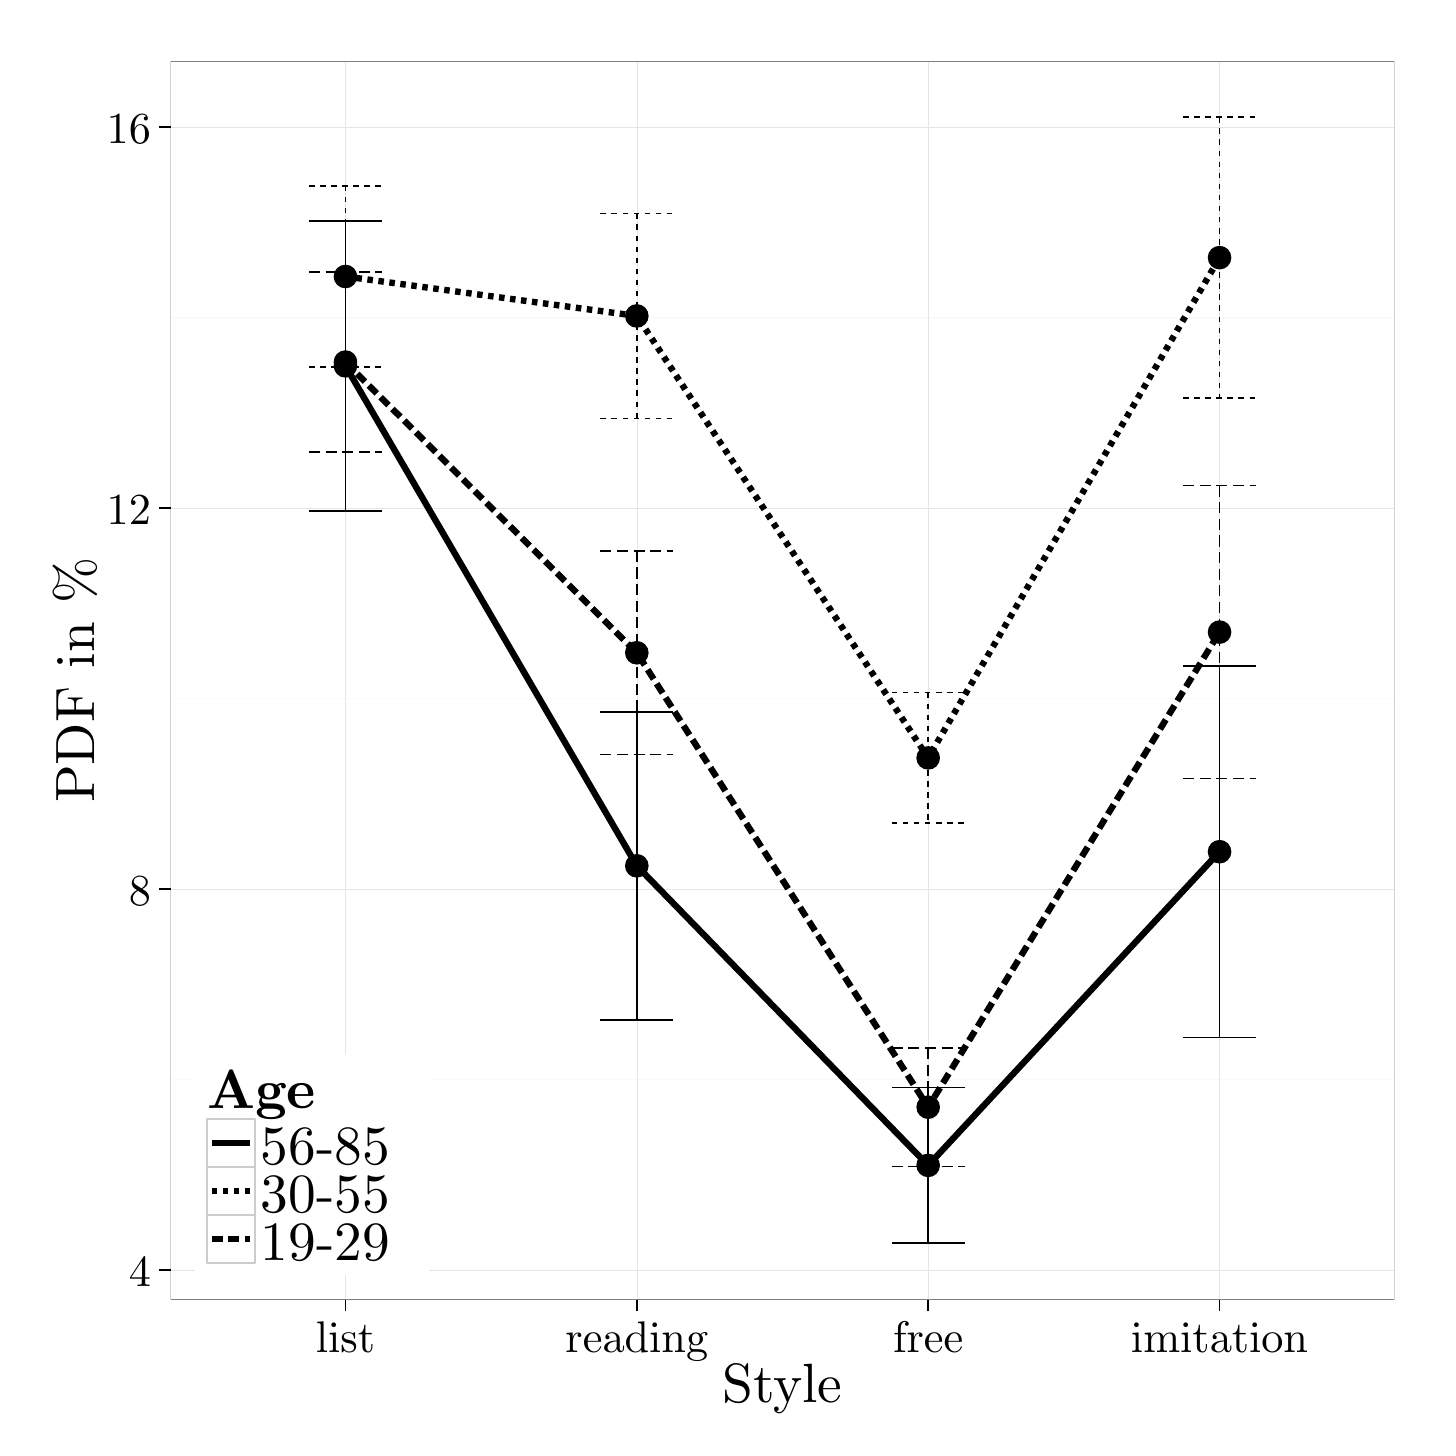
\begin{tikzpicture}[x=1pt,y=1pt]
\definecolor{fillColor}{RGB}{255,255,255}
\path[use as bounding box,fill=fillColor,fill opacity=0.00] (0,0) rectangle (505.89,505.89);
\begin{scope}
\path[clip] (  0.00,  0.00) rectangle (505.89,505.89);
\definecolor{drawColor}{RGB}{255,255,255}
\definecolor{fillColor}{RGB}{255,255,255}

\path[draw=drawColor,line width= 0.6pt,line join=round,line cap=round,fill=fillColor] (  0.00, -0.00) rectangle (505.89,505.89);
\end{scope}
\begin{scope}
\path[clip] ( 51.66, 46.31) rectangle (493.85,493.84);
\definecolor{fillColor}{RGB}{255,255,255}

\path[fill=fillColor] ( 51.66, 46.31) rectangle (493.84,493.84);
\definecolor{drawColor}{gray}{0.98}

\path[draw=drawColor,line width= 0.6pt,line join=round] ( 51.66,125.81) --
	(493.85,125.81);

\path[draw=drawColor,line width= 0.6pt,line join=round] ( 51.66,263.45) --
	(493.85,263.45);

\path[draw=drawColor,line width= 0.6pt,line join=round] ( 51.66,401.09) --
	(493.85,401.09);
\definecolor{drawColor}{gray}{0.90}

\path[draw=drawColor,line width= 0.2pt,line join=round] ( 51.66, 56.99) --
	(493.85, 56.99);

\path[draw=drawColor,line width= 0.2pt,line join=round] ( 51.66,194.63) --
	(493.85,194.63);

\path[draw=drawColor,line width= 0.2pt,line join=round] ( 51.66,332.27) --
	(493.85,332.27);

\path[draw=drawColor,line width= 0.2pt,line join=round] ( 51.66,469.91) --
	(493.85,469.91);

\path[draw=drawColor,line width= 0.2pt,line join=round] (114.83, 46.31) --
	(114.83,493.84);

\path[draw=drawColor,line width= 0.2pt,line join=round] (220.11, 46.31) --
	(220.11,493.84);

\path[draw=drawColor,line width= 0.2pt,line join=round] (325.39, 46.31) --
	(325.39,493.84);

\path[draw=drawColor,line width= 0.2pt,line join=round] (430.68, 46.31) --
	(430.68,493.84);
\definecolor{fillColor}{RGB}{0,0,0}

\path[fill=fillColor] (114.83,383.68) circle (  4.27);

\path[fill=fillColor] (114.83,415.97) circle (  4.27);

\path[fill=fillColor] (114.83,385.05) circle (  4.27);

\path[fill=fillColor] (220.11,203.03) circle (  4.27);

\path[fill=fillColor] (220.11,401.72) circle (  4.27);

\path[fill=fillColor] (220.11,280.00) circle (  4.27);

\path[fill=fillColor] (325.39, 94.77) circle (  4.27);

\path[fill=fillColor] (325.39,242.02) circle (  4.27);

\path[fill=fillColor] (325.39,115.81) circle (  4.27);

\path[fill=fillColor] (430.68,208.12) circle (  4.27);

\path[fill=fillColor] (430.68,422.79) circle (  4.27);

\path[fill=fillColor] (430.68,287.48) circle (  4.27);
\definecolor{drawColor}{RGB}{0,0,0}

\path[draw=drawColor,line width= 2.3pt,line join=round] (114.83,383.68) --
	(220.11,203.03) --
	(325.39, 94.77) --
	(430.68,208.12);

\path[draw=drawColor,line width= 2.3pt,dash pattern=on 2pt off 2pt ,line join=round] (114.83,415.97) --
	(220.11,401.72) --
	(325.39,242.02) --
	(430.68,422.79);

\path[draw=drawColor,line width= 2.3pt,dash pattern=on 4pt off 2pt ,line join=round] (114.83,385.05) --
	(220.11,280.00) --
	(325.39,115.81) --
	(430.68,287.48);

\path[draw=drawColor,line width= 0.6pt,line join=round] (101.67,436.02) --
	(127.99,436.02);

\path[draw=drawColor,line width= 0.6pt,line join=round] (114.83,436.02) --
	(114.83,331.33);

\path[draw=drawColor,line width= 0.6pt,line join=round] (101.67,331.33) --
	(127.99,331.33);

\path[draw=drawColor,line width= 0.6pt,line join=round] (206.95,258.70) --
	(233.27,258.70);

\path[draw=drawColor,line width= 0.6pt,line join=round] (220.11,258.70) --
	(220.11,147.36);

\path[draw=drawColor,line width= 0.6pt,line join=round] (206.95,147.36) --
	(233.27,147.36);

\path[draw=drawColor,line width= 0.6pt,line join=round] (312.23,122.88) --
	(338.55,122.88);

\path[draw=drawColor,line width= 0.6pt,line join=round] (325.39,122.88) --
	(325.39, 66.65);

\path[draw=drawColor,line width= 0.6pt,line join=round] (312.23, 66.65) --
	(338.55, 66.65);

\path[draw=drawColor,line width= 0.6pt,line join=round] (417.52,275.28) --
	(443.84,275.28);

\path[draw=drawColor,line width= 0.6pt,line join=round] (430.68,275.28) --
	(430.68,140.96);

\path[draw=drawColor,line width= 0.6pt,line join=round] (417.52,140.96) --
	(443.84,140.96);

\path[draw=drawColor,line width= 0.6pt,dash pattern=on 2pt off 2pt ,line join=round] (101.67,448.74) --
	(127.99,448.74);

\path[draw=drawColor,line width= 0.6pt,dash pattern=on 2pt off 2pt ,line join=round] (114.83,448.74) --
	(114.83,383.19);

\path[draw=drawColor,line width= 0.6pt,dash pattern=on 2pt off 2pt ,line join=round] (101.67,383.19) --
	(127.99,383.19);

\path[draw=drawColor,line width= 0.6pt,dash pattern=on 2pt off 2pt ,line join=round] (206.95,438.78) --
	(233.27,438.78);

\path[draw=drawColor,line width= 0.6pt,dash pattern=on 2pt off 2pt ,line join=round] (220.11,438.78) --
	(220.11,364.66);

\path[draw=drawColor,line width= 0.6pt,dash pattern=on 2pt off 2pt ,line join=round] (206.95,364.66) --
	(233.27,364.66);

\path[draw=drawColor,line width= 0.6pt,dash pattern=on 2pt off 2pt ,line join=round] (312.23,265.61) --
	(338.55,265.61);

\path[draw=drawColor,line width= 0.6pt,dash pattern=on 2pt off 2pt ,line join=round] (325.39,265.61) --
	(325.39,218.43);

\path[draw=drawColor,line width= 0.6pt,dash pattern=on 2pt off 2pt ,line join=round] (312.23,218.43) --
	(338.55,218.43);

\path[draw=drawColor,line width= 0.6pt,dash pattern=on 2pt off 2pt ,line join=round] (417.52,473.50) --
	(443.84,473.50);

\path[draw=drawColor,line width= 0.6pt,dash pattern=on 2pt off 2pt ,line join=round] (430.68,473.50) --
	(430.68,372.07);

\path[draw=drawColor,line width= 0.6pt,dash pattern=on 2pt off 2pt ,line join=round] (417.52,372.07) --
	(443.84,372.07);

\path[draw=drawColor,line width= 0.6pt,dash pattern=on 4pt off 2pt ,line join=round] (101.67,417.59) --
	(127.99,417.59);

\path[draw=drawColor,line width= 0.6pt,dash pattern=on 4pt off 2pt ,line join=round] (114.83,417.59) --
	(114.83,352.51);

\path[draw=drawColor,line width= 0.6pt,dash pattern=on 4pt off 2pt ,line join=round] (101.67,352.51) --
	(127.99,352.51);

\path[draw=drawColor,line width= 0.6pt,dash pattern=on 4pt off 2pt ,line join=round] (206.95,316.82) --
	(233.27,316.82);

\path[draw=drawColor,line width= 0.6pt,dash pattern=on 4pt off 2pt ,line join=round] (220.11,316.82) --
	(220.11,243.19);

\path[draw=drawColor,line width= 0.6pt,dash pattern=on 4pt off 2pt ,line join=round] (206.95,243.19) --
	(233.27,243.19);

\path[draw=drawColor,line width= 0.6pt,dash pattern=on 4pt off 2pt ,line join=round] (312.23,137.19) --
	(338.55,137.19);

\path[draw=drawColor,line width= 0.6pt,dash pattern=on 4pt off 2pt ,line join=round] (325.39,137.19) --
	(325.39, 94.42);

\path[draw=drawColor,line width= 0.6pt,dash pattern=on 4pt off 2pt ,line join=round] (312.23, 94.42) --
	(338.55, 94.42);

\path[draw=drawColor,line width= 0.6pt,dash pattern=on 4pt off 2pt ,line join=round] (417.52,340.39) --
	(443.84,340.39);

\path[draw=drawColor,line width= 0.6pt,dash pattern=on 4pt off 2pt ,line join=round] (430.68,340.39) --
	(430.68,234.58);

\path[draw=drawColor,line width= 0.6pt,dash pattern=on 4pt off 2pt ,line join=round] (417.52,234.58) --
	(443.84,234.58);
\definecolor{drawColor}{gray}{0.50}

\path[draw=drawColor,line width= 0.6pt,line join=round,line cap=round] ( 51.66, 46.31) rectangle (493.84,493.84);
\end{scope}
\begin{scope}
\path[clip] (  0.00,  0.00) rectangle (505.89,505.89);
\definecolor{drawColor}{RGB}{0,0,0}

\node[text=drawColor,anchor=base east,inner sep=0pt, outer sep=0pt, scale=  1.60] at ( 44.55, 50.96) {4};

\node[text=drawColor,anchor=base east,inner sep=0pt, outer sep=0pt, scale=  1.60] at ( 44.55,188.60) {8};

\node[text=drawColor,anchor=base east,inner sep=0pt, outer sep=0pt, scale=  1.60] at ( 44.55,326.24) {12};

\node[text=drawColor,anchor=base east,inner sep=0pt, outer sep=0pt, scale=  1.60] at ( 44.55,463.88) {16};
\end{scope}
\begin{scope}
\path[clip] (  0.00,  0.00) rectangle (505.89,505.89);
\definecolor{drawColor}{RGB}{0,0,0}

\path[draw=drawColor,line width= 0.6pt,line join=round] ( 47.39, 56.99) --
	( 51.66, 56.99);

\path[draw=drawColor,line width= 0.6pt,line join=round] ( 47.39,194.63) --
	( 51.66,194.63);

\path[draw=drawColor,line width= 0.6pt,line join=round] ( 47.39,332.27) --
	( 51.66,332.27);

\path[draw=drawColor,line width= 0.6pt,line join=round] ( 47.39,469.91) --
	( 51.66,469.91);
\end{scope}
\begin{scope}
\path[clip] (  0.00,  0.00) rectangle (505.89,505.89);
\definecolor{drawColor}{RGB}{0,0,0}

\path[draw=drawColor,line width= 0.6pt,line join=round] (114.83, 42.04) --
	(114.83, 46.31);

\path[draw=drawColor,line width= 0.6pt,line join=round] (220.11, 42.04) --
	(220.11, 46.31);

\path[draw=drawColor,line width= 0.6pt,line join=round] (325.39, 42.04) --
	(325.39, 46.31);

\path[draw=drawColor,line width= 0.6pt,line join=round] (430.68, 42.04) --
	(430.68, 46.31);
\end{scope}
\begin{scope}
\path[clip] (  0.00,  0.00) rectangle (505.89,505.89);
\definecolor{drawColor}{RGB}{0,0,0}

\node[text=drawColor,anchor=base,inner sep=0pt, outer sep=0pt, scale=  1.60] at (114.83, 27.13) {list};

\node[text=drawColor,anchor=base,inner sep=0pt, outer sep=0pt, scale=  1.60] at (220.11, 27.13) {reading};

\node[text=drawColor,anchor=base,inner sep=0pt, outer sep=0pt, scale=  1.60] at (325.39, 27.13) {free};

\node[text=drawColor,anchor=base,inner sep=0pt, outer sep=0pt, scale=  1.60] at (430.68, 27.13) {imitation};
\end{scope}
\begin{scope}
\path[clip] (  0.00,  0.00) rectangle (505.89,505.89);
\definecolor{drawColor}{RGB}{0,0,0}

\node[text=drawColor,anchor=base,inner sep=0pt, outer sep=0pt, scale=  2.00] at (272.75,  9.03) {Style};
\end{scope}
\begin{scope}
\path[clip] (  0.00,  0.00) rectangle (505.89,505.89);
\definecolor{drawColor}{RGB}{0,0,0}

\node[text=drawColor,rotate= 90.00,anchor=base,inner sep=0pt, outer sep=0pt, scale=  2.00] at ( 24.12,270.08) {PDF in {\%}};
\end{scope}
\begin{scope}
\path[clip] (  0.00,  0.00) rectangle (505.89,505.89);
\definecolor{fillColor}{RGB}{255,255,255}

\path[fill=fillColor] ( 60.53, 55.18) rectangle (144.95,134.50);
\end{scope}
\begin{scope}
\path[clip] (  0.00,  0.00) rectangle (505.89,505.89);
\definecolor{drawColor}{RGB}{0,0,0}

\node[text=drawColor,anchor=base west,inner sep=0pt, outer sep=0pt, scale=  2.00] at ( 64.80,115.48) {\bfseries Age};
\end{scope}
\begin{scope}
\path[clip] (  0.00,  0.00) rectangle (505.89,505.89);
\definecolor{drawColor}{gray}{0.80}
\definecolor{fillColor}{RGB}{255,255,255}

\path[draw=drawColor,line width= 0.6pt,line join=round,line cap=round,fill=fillColor] ( 64.80, 94.13) rectangle ( 82.14,111.48);
\end{scope}
\begin{scope}
\path[clip] (  0.00,  0.00) rectangle (505.89,505.89);
\definecolor{drawColor}{RGB}{0,0,0}

\path[draw=drawColor,line width= 2.3pt,line join=round] ( 66.53,102.81) -- ( 80.41,102.81);
\end{scope}
\begin{scope}
\path[clip] (  0.00,  0.00) rectangle (505.89,505.89);
\definecolor{drawColor}{RGB}{0,0,0}

\path[draw=drawColor,line width= 0.6pt,line join=round] ( 66.53,102.81) -- ( 80.41,102.81);
\end{scope}
\begin{scope}
\path[clip] (  0.00,  0.00) rectangle (505.89,505.89);
\definecolor{drawColor}{gray}{0.80}
\definecolor{fillColor}{RGB}{255,255,255}

\path[draw=drawColor,line width= 0.6pt,line join=round,line cap=round,fill=fillColor] ( 64.80, 76.79) rectangle ( 82.14, 94.13);
\end{scope}
\begin{scope}
\path[clip] (  0.00,  0.00) rectangle (505.89,505.89);
\definecolor{drawColor}{RGB}{0,0,0}

\path[draw=drawColor,line width= 2.3pt,dash pattern=on 2pt off 2pt ,line join=round] ( 66.53, 85.46) -- ( 80.41, 85.46);
\end{scope}
\begin{scope}
\path[clip] (  0.00,  0.00) rectangle (505.89,505.89);
\definecolor{drawColor}{RGB}{0,0,0}

\path[draw=drawColor,line width= 0.6pt,dash pattern=on 2pt off 2pt ,line join=round] ( 66.53, 85.46) -- ( 80.41, 85.46);
\end{scope}
\begin{scope}
\path[clip] (  0.00,  0.00) rectangle (505.89,505.89);
\definecolor{drawColor}{gray}{0.80}
\definecolor{fillColor}{RGB}{255,255,255}

\path[draw=drawColor,line width= 0.6pt,line join=round,line cap=round,fill=fillColor] ( 64.80, 59.44) rectangle ( 82.14, 76.79);
\end{scope}
\begin{scope}
\path[clip] (  0.00,  0.00) rectangle (505.89,505.89);
\definecolor{drawColor}{RGB}{0,0,0}

\path[draw=drawColor,line width= 2.3pt,dash pattern=on 4pt off 2pt ,line join=round] ( 66.53, 68.12) -- ( 80.41, 68.12);
\end{scope}
\begin{scope}
\path[clip] (  0.00,  0.00) rectangle (505.89,505.89);
\definecolor{drawColor}{RGB}{0,0,0}

\path[draw=drawColor,line width= 0.6pt,dash pattern=on 4pt off 2pt ,line join=round] ( 66.53, 68.12) -- ( 80.41, 68.12);
\end{scope}
\begin{scope}
\path[clip] (  0.00,  0.00) rectangle (505.89,505.89);
\definecolor{drawColor}{RGB}{0,0,0}

\node[text=drawColor,anchor=base west,inner sep=0pt, outer sep=0pt, scale=  2.00] at ( 84.31, 95.26) {56-85};
\end{scope}
\begin{scope}
\path[clip] (  0.00,  0.00) rectangle (505.89,505.89);
\definecolor{drawColor}{RGB}{0,0,0}

\node[text=drawColor,anchor=base west,inner sep=0pt, outer sep=0pt, scale=  2.00] at ( 84.31, 77.92) {30-55};
\end{scope}
\begin{scope}
\path[clip] (  0.00,  0.00) rectangle (505.89,505.89);
\definecolor{drawColor}{RGB}{0,0,0}

\node[text=drawColor,anchor=base west,inner sep=0pt, outer sep=0pt, scale=  2.00] at ( 84.31, 60.57) {19-29};
\end{scope}
\end{tikzpicture}
} 
	\caption{/ŋ(g)/: PDF by style ([ɪn] excluded)}
	\label{fig.line.ng.tot}
\end{figure}

The last predictor we will look at is again the style dimension (\figref{fig.line.ng.tot}), where we find something interesting going on.
Not only is there a very clear pattern, but this pattern is essentially identical for all three speaker groups investigated, which is the reason why the mixed linear effects regression did not find a significant interaction of style and age.
The pattern we see is not prototypical Labovian \isi{style shifting}, however.
If it were, use of the local variant of /ŋ(g)/ would decrease in more formal contexts like reading a text or a word list.
Instead, the data show that velar nasal plus is more \emph{common} in those formal contexts.
Both the oldest and the youngest speakers in the sample have means in spontaneous speech, the reading passage, and the word list which are all significantly different from one another (cf. the standard error whiskers, which do not overlap between the styles and within each age group).
The only difference that is found for the middle-aged speakers in this respect is that the text passage and the word lists are statistically identical, but these two formal registers are nevertheless significantly different from free speech.

On the other hand, there is an undeniable rise from spontaneous speech towards accent perform\is{accent performance}ance.
When subjects are asked to put on a particularly strong Scouse accent they \emph{do} make use of velar nasal plus to a certain extent.
Compared to free speech, realisations during the accent imitation\is{accent performance} are clearly significantly more Scouse, irrespective of age group; \isi{PDF} reaches about the same level as when people read out a text, a register which `imitation\is{accent performance}' is not significantly different from (cf. again the (lack of) overlap in the standard error whiskers in \figref{fig.line.ng.tot}).
This graph is somewhat reminiscent of the corresponding figure that was generated for F1 measurements of happ\textsc{y} (\figref{fig.line.f1w.happy.tot} on page \pageref{fig.line.f1w.happy.tot}), which also revealed more Scouse values for both the word list and accent imitation\is{accent performance} when compared to reading and spontaneous speech.
It was noted earlier that observations for the register `word list' only come from contexts that seem to favour higher \isi{PDF} values generally and this could explain at least parts of the rise from `reading' to `word list'.
It fails, however, to account for the differences between the other three styles, where these \isi{phonological context}s make up about the same proportion of tokens.
Just as in the case of happ\textsc{y}, some additional explanation is needed here (see Chapter \ref{ch.prod_discussion}).

\section{/k/}
\label{prod.res.con.k}

\subsection{Overview}
\label{sec.prod.res.con.k.overview}

Just as with velar nasal plus, a mixed linear effects model was fit to the data for /k/.
Unreleased /k/'s were not included in the model, because these realisations are probably more phonologically than socially conditioned, meaning that, compared to the plosive-fricative continuum, speakers do not have the same degree of choice when to use this variant.
The maximal model contained more \isi{collinearity} than is generally deemed acceptable (κ = 18.8), but once again much of it was unproblematic because it was only caused by the two three-way interactions, as a separate model without these revealed (κ = 12.25).
The original maximal model (including the interactions) was therefore retained and served as the point of departure for model selection based on AIC scores and F-tests comparing nested models.
The final, reduced model (based on 2862 observations) is reprinted below (\tabref{tab.regression.k}, R\textsuperscript{2}-equivalent = 0.37).

{\footnotesize
	\begin{longtable}[c]{p{0.3\textwidth}rrrrrl}
				\caption{/k/: mixed linear effects regression}\label{tab.regression.k}\\
		\hline
		Fixed effects: & Estimate & Std. Error & df & t value & Pr($>$$|$t$|$) & \\
		\hline
		(Intercept) & 58.07 & 1.49 & 142.04 & 39.13 & < 0.001 & *** \\ 
		STYLElist & -11.44 & 1.70 & 884.38 & -6.57 & < 0.001 & *** \\ 
		STYLEread & -2.27 & 1.28 & 1729.76 & -1.71 & 0.09 & . \\ 
		STYLEfree & -3.79 & 1.10 & 470.85 & -3.21 & < 0.01 & ** \\ 
		AGE56-85 & 0.74 & 1.13 & 2761.75 & 0.36 & 0.72 & \\ 
		AGE30-55 & -0.21 & 0.95 & 2758.04 & -0.08 & 0.94 & \\ 
		GENDERf & -5.53 & 0.71 & 2742.23 & -7.78 & < 0.001 & *** \\ 
		CLASSmc & -4.83 & 0.71 & 2749.02 & -6.58 & < 0.001 & *** \\ 
		ENVIRV\_V & 18.76 & 1.73 & 124.75 & 10.62 & < 0.001 & *** \\ 
		ENVIRV\_\#V & 8.22 & 1.31 & 1982.48 & 6.30 & < 0.001 & *** \\ 
		ENVIRV\_\#gli & 9.64 & 2.21 & 2699.98 & 4.34 & < 0.001 & *** \\ 
		ENVIRV\_\# & 10.24 & 1.29 & 1339.82 & 7.87 & < 0.001 & *** \\ 
		ENVIRV\_\#liq & 6.53 & 3.95 & 2798.38 & 1.78 & 0.08 & . \\ 
		ENVIRV\_\#nas & 10.43 & 3.05 & 2745.07 & 3.43 & < 0.001 & *** \\ 
		ENVIRV\_\#vdfric & -13.69 & 2.14 & 2706.45 & -6.38 & < 0.001 & *** \\ 
		ENVIRV\_\#vlfric & -15.04 & 2.06 & 2581.56 & -7.23 & < 0.001 & *** \\ 
		ENVIRV\_\#vdplos & -2.29 & 2.85 & 2737.97 & -0.81 & 0.42 & \\ 
		ENVIRV\_\#vlplos & -13.86 & 2.60 & 2372.19 & -5.33 & < 0.001 & *** \\ 
		STYLElist:AGE56-85 & 0.83 & 2.21 & 2723.94 & 0.53 & 0.59 & \\ 
		STYLEread:AGE56-85 & -1.26 & 1.85 & 2734.49 & -0.49 & 0.62 & \\ 
		STYLEfree:AGE56-85 & -2.86 & 1.33 & 2815.49 & -1.93 & 0.05 & . \\ 
		STYLElist:AGE30-55 & 4.17 & 1.92 & 2721.76 & 2.10 & 0.04 & * \\ 
		STYLEread:AGE30-55 & 0.31 & 1.56 & 2735.38 & 0.11 & 0.91 & \\ 
		STYLEfree:AGE30-55 & -0.74 & 1.09 & 2796.95 & -0.90 & 0.37 & \\ 
		STYLElist:GENDERf & -3.39 & 1.42 & 2718.38 & -2.36 & 0.02 & * \\ 
		STYLEread:GENDERf & -2.14 & 1.17 & 2731.10 & -1.81 & 0.07 & . \\ 
		STYLEfree:GENDERf & 0.47 & 0.86 & 2804.23 & 0.46 & 0.64 & \\ 
		STYLElist:CLASSmc & -0.50 & 1.43 & 2721.77 & -0.47 & 0.64 & \\ 
		STYLEread:CLASSmc & -1.15 & 1.18 & 2734.34 & -1.12 & 0.26 & \\ 
		STYLEfree:CLASSmc & -2.16 & 0.85 & 2807.04 & -2.77 & 0.01 & ** \\ 
		AGE56-85:GENDERf & -4.76 & 1.11 & 2735.66 & -4.25 & < 0.001 & *** \\ 
		AGE30-55:GENDERf & 5.24 & 0.98 & 2749.75 & 5.34 & < 0.001 & *** \\ 
		AGE56-85:CLASSmc & 6.00 & 1.12 & 2754.82 & 5.70 & < 0.001 & *** \\ 
		AGE30-55:CLASSmc & -1.72 & 0.99 & 2752.61 & -1.94 & 0.05 & . \\ 
		GENDERf:CLASSmc & -2.66 & 0.51 & 2826.51 & -5.31 & < 0.001 & *** \\ 
		STYLElist:AGE56-85:GENDERf & -0.80 & 2.22 & 2718.25 & -0.37 & 0.71 & \\ 
		STYLEread:AGE56-85:GENDERf & -6.89 & 1.85 & 2725.93 & -3.73 & < 0.001 & *** \\ 
		STYLEfree:AGE56-85:GENDERf & -0.91 & 1.35 & 2800.05 & -0.64 & 0.53 & \\ 
		STYLElist:AGE30-55:GENDERf & -1.14 & 1.95 & 2722.26 & -0.58 & 0.56 & \\ 
		STYLEread:AGE30-55:GENDERf & 8.13 & 1.58 & 2731.42 & 5.16 & < 0.001 & *** \\ 
		STYLEfree:AGE30-55:GENDERf & 0.99 & 1.14 & 2802.97 & 0.84 & 0.40 & \\ 
		STYLElist:AGE56-85:CLASSmc & 2.39 & 2.22 & 2722.27 & 0.92 & 0.36 & \\ 
		STYLEread:AGE56-85:CLASSmc & 2.48 & 1.85 & 2731.52 & 1.16 & 0.25 & \\ 
		STYLEfree:AGE56-85:CLASSmc & 1.71 & 1.37 & 2811.58 & 1.03 & 0.30 & \\ 
		STYLElist:AGE30-55:CLASSmc & -5.56 & 1.95 & 2723.95 & -2.75 & 0.01 & ** \\ 
		STYLEread:AGE30-55:CLASSmc & -1.18 & 1.58 & 2732.59 & -0.63 & 0.53 & \\ 
		STYLEfree:AGE30-55:CLASSmc & 4.35 & 1.16 & 2801.01 & 3.85 & < 0.001 & *** \\
		\hline
		Random effects: & \multicolumn{6}{l}{(number of obs: 2862, groups: WORD, 217)} \\
		Groups &         Name & Variance &      Std.Dev. & & & \\
		WORD &  (Intercept) & 39.400 & 6.277 & & & \\
		Residual  &         & 551.900 & 23.493 & & & \\
		\hline
	\end{longtable}
}

This model is (by far, in most cases) the one that contains the greatest number of significant predictors in this study.
In fact, only one factor was eliminated as non-significant, namely \isi{frequency} of the keyword.
Age of the speaker does not reach significance as a main effect (but see \sectref{sec.prod.res.con.k.agegender} for some thoughts on this), but it does appear in numerous interactions which do and was therefore retained.
All the other extralinguistic factors (as well as phonological environment\is{phonological context} of the dependent variable) are found to be significant main effects.
In addition, every single one of the two- and three-way interactions mentioned in \sectref{sec.prod_method.stats} is found to have a statistically robust impact on \isi{PDF} measurements of /k/ in this sample.

\subsection{Phonological context}
\label{sec.prod.res.con.k.phon}

\begin{figure}[h]
	\centering
		\definecolor{shadecolor}{rgb}{0.969, 0.969, 0.969}
		\resizebox{0.5\linewidth}{!}{% Created by tikzDevice version 0.8.1 on 2016-02-09 02:17:13
% !TEX encoding = UTF-8 Unicode
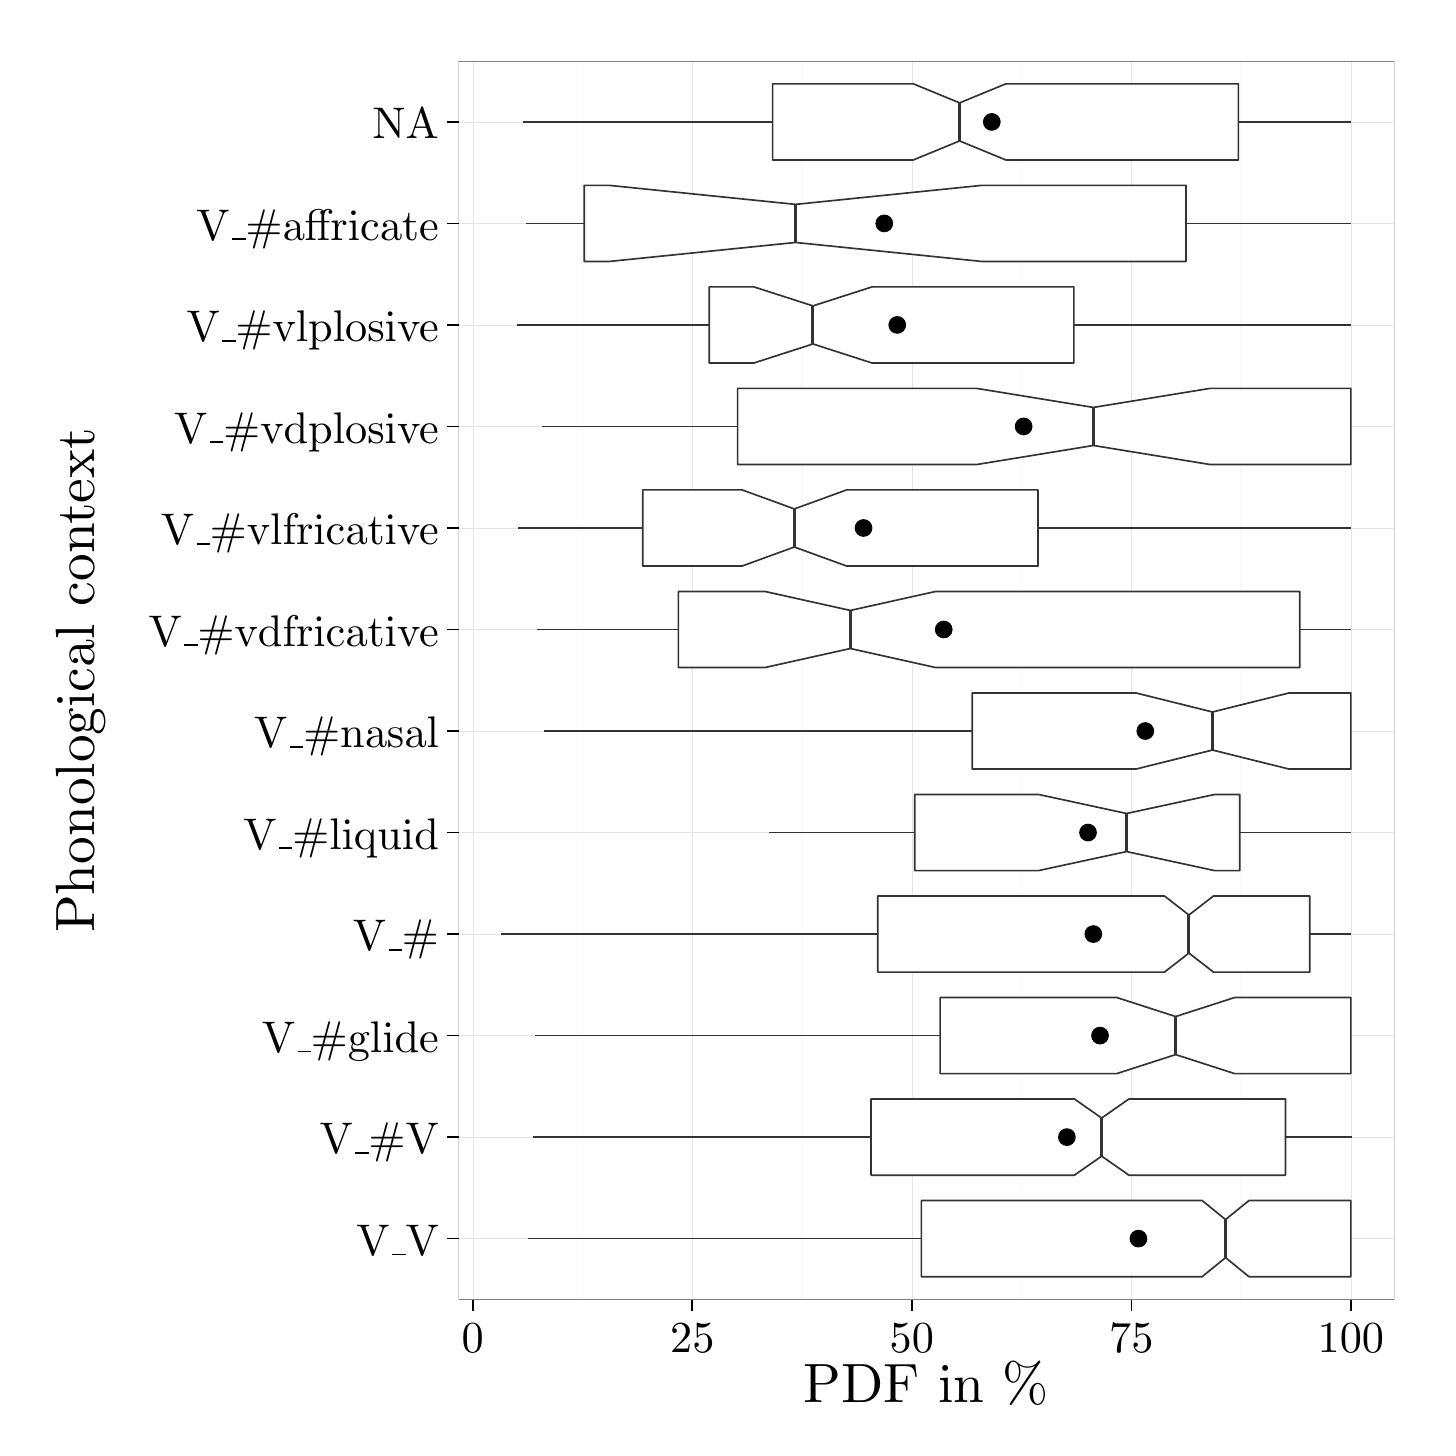
\begin{tikzpicture}[x=1pt,y=1pt]
\definecolor{fillColor}{RGB}{255,255,255}
\path[use as bounding box,fill=fillColor,fill opacity=0.00] (0,0) rectangle (505.89,505.89);
\begin{scope}
\path[clip] (  0.00,  0.00) rectangle (505.89,505.89);
\definecolor{drawColor}{RGB}{255,255,255}
\definecolor{fillColor}{RGB}{255,255,255}

\path[draw=drawColor,line width= 0.6pt,line join=round,line cap=round,fill=fillColor] (  0.00, -0.00) rectangle (505.89,505.89);
\end{scope}
\begin{scope}
\path[clip] (155.70, 46.31) rectangle (493.85,493.84);
\definecolor{fillColor}{RGB}{255,255,255}

\path[fill=fillColor] (155.70, 46.31) rectangle (493.85,493.84);
\definecolor{drawColor}{gray}{0.98}

\path[draw=drawColor,line width= 0.6pt,line join=round] (200.51, 46.31) --
	(200.51,493.84);

\path[draw=drawColor,line width= 0.6pt,line join=round] (279.83, 46.31) --
	(279.83,493.84);

\path[draw=drawColor,line width= 0.6pt,line join=round] (359.15, 46.31) --
	(359.15,493.84);

\path[draw=drawColor,line width= 0.6pt,line join=round] (438.47, 46.31) --
	(438.47,493.84);
\definecolor{drawColor}{gray}{0.90}

\path[draw=drawColor,line width= 0.2pt,line join=round] (155.70, 68.32) --
	(493.85, 68.32);

\path[draw=drawColor,line width= 0.2pt,line join=round] (155.70,105.00) --
	(493.85,105.00);

\path[draw=drawColor,line width= 0.2pt,line join=round] (155.70,141.68) --
	(493.85,141.68);

\path[draw=drawColor,line width= 0.2pt,line join=round] (155.70,178.37) --
	(493.85,178.37);

\path[draw=drawColor,line width= 0.2pt,line join=round] (155.70,215.05) --
	(493.85,215.05);

\path[draw=drawColor,line width= 0.2pt,line join=round] (155.70,251.73) --
	(493.85,251.73);

\path[draw=drawColor,line width= 0.2pt,line join=round] (155.70,288.42) --
	(493.85,288.42);

\path[draw=drawColor,line width= 0.2pt,line join=round] (155.70,325.10) --
	(493.85,325.10);

\path[draw=drawColor,line width= 0.2pt,line join=round] (155.70,361.78) --
	(493.85,361.78);

\path[draw=drawColor,line width= 0.2pt,line join=round] (155.70,398.47) --
	(493.85,398.47);

\path[draw=drawColor,line width= 0.2pt,line join=round] (155.70,435.15) --
	(493.85,435.15);

\path[draw=drawColor,line width= 0.2pt,line join=round] (155.70,471.83) --
	(493.85,471.83);

\path[draw=drawColor,line width= 0.2pt,line join=round] (160.85, 46.31) --
	(160.85,493.84);

\path[draw=drawColor,line width= 0.2pt,line join=round] (240.17, 46.31) --
	(240.17,493.84);

\path[draw=drawColor,line width= 0.2pt,line join=round] (319.49, 46.31) --
	(319.49,493.84);

\path[draw=drawColor,line width= 0.2pt,line join=round] (398.81, 46.31) --
	(398.81,493.84);

\path[draw=drawColor,line width= 0.2pt,line join=round] (478.13, 46.31) --
	(478.13,493.84);
\definecolor{drawColor}{gray}{0.20}

\path[draw=drawColor,line width= 0.6pt,line join=round] (478.13, 68.32) -- (478.13, 68.32);

\path[draw=drawColor,line width= 0.6pt,line join=round] (322.95, 68.32) -- (180.74, 68.32);

\path[draw=drawColor,line width= 0.6pt,line join=round,line cap=round,fill=fillColor] (478.13, 54.56) --
	(441.31, 54.56) --
	(432.85, 61.44) --
	(424.39, 54.56) --
	(322.95, 54.56) --
	(322.95, 82.07) --
	(424.39, 82.07) --
	(432.85, 75.20) --
	(441.31, 82.07) --
	(478.13, 82.07) --
	(478.13, 54.56) --
	cycle;

\path[draw=drawColor,line width= 1.1pt,line join=round] (432.85, 61.44) -- (432.85, 75.20);

\path[draw=drawColor,line width= 0.6pt,line join=round] (454.50,105.00) -- (478.47,105.00);

\path[draw=drawColor,line width= 0.6pt,line join=round] (304.74,105.00) -- (182.52,105.00);

\path[draw=drawColor,line width= 0.6pt,line join=round,line cap=round,fill=fillColor] (454.50, 91.24) --
	(397.92, 91.24) --
	(388.08, 98.12) --
	(378.24, 91.24) --
	(304.74, 91.24) --
	(304.74,118.76) --
	(378.24,118.76) --
	(388.08,111.88) --
	(397.92,118.76) --
	(454.50,118.76) --
	(454.50, 91.24) --
	cycle;

\path[draw=drawColor,line width= 1.1pt,line join=round] (388.08, 98.12) -- (388.08,111.88);

\path[draw=drawColor,line width= 0.6pt,line join=round] (478.13,141.68) -- (478.13,141.68);

\path[draw=drawColor,line width= 0.6pt,line join=round] (329.70,141.68) -- (183.50,141.68);

\path[draw=drawColor,line width= 0.6pt,line join=round,line cap=round,fill=fillColor] (478.13,127.93) --
	(436.15,127.93) --
	(414.83,134.81) --
	(393.51,127.93) --
	(329.70,127.93) --
	(329.70,155.44) --
	(393.51,155.44) --
	(414.83,148.56) --
	(436.15,155.44) --
	(478.13,155.44) --
	(478.13,127.93) --
	cycle;

\path[draw=drawColor,line width= 1.1pt,line join=round] (414.83,134.81) -- (414.83,148.56);

\path[draw=drawColor,line width= 0.6pt,line join=round] (463.28,178.37) -- (478.13,178.37);

\path[draw=drawColor,line width= 0.6pt,line join=round] (307.18,178.37) -- (171.07,178.37);

\path[draw=drawColor,line width= 0.6pt,line join=round,line cap=round,fill=fillColor] (463.28,164.61) --
	(428.48,164.61) --
	(419.62,171.49) --
	(410.76,164.61) --
	(307.18,164.61) --
	(307.18,192.12) --
	(410.76,192.12) --
	(419.62,185.25) --
	(428.48,192.12) --
	(463.28,192.12) --
	(463.28,164.61) --
	cycle;

\path[draw=drawColor,line width= 1.1pt,line join=round] (419.62,171.49) -- (419.62,185.25);

\path[draw=drawColor,line width= 0.6pt,line join=round] (437.99,215.05) -- (478.13,215.05);

\path[draw=drawColor,line width= 0.6pt,line join=round] (320.54,215.05) -- (267.87,215.05);

\path[draw=drawColor,line width= 0.6pt,line join=round,line cap=round,fill=fillColor] (437.99,201.29) --
	(428.92,201.29) --
	(397.09,208.17) --
	(365.27,201.29) --
	(320.54,201.29) --
	(320.54,228.81) --
	(365.27,228.81) --
	(397.09,221.93) --
	(428.92,228.81) --
	(437.99,228.81) --
	(437.99,201.29) --
	cycle;

\path[draw=drawColor,line width= 1.1pt,line join=round] (397.09,208.17) -- (397.09,221.93);

\path[draw=drawColor,line width= 0.6pt,line join=round] (478.13,251.73) -- (478.13,251.73);

\path[draw=drawColor,line width= 0.6pt,line join=round] (341.29,251.73) -- (186.65,251.73);

\path[draw=drawColor,line width= 0.6pt,line join=round,line cap=round,fill=fillColor] (478.13,237.98) --
	(455.81,237.98) --
	(428.12,244.86) --
	(400.44,237.98) --
	(341.29,237.98) --
	(341.29,265.49) --
	(400.44,265.49) --
	(428.12,258.61) --
	(455.81,265.49) --
	(478.13,265.49) --
	(478.13,237.98) --
	cycle;

\path[draw=drawColor,line width= 1.1pt,line join=round] (428.12,244.86) -- (428.12,258.61);

\path[draw=drawColor,line width= 0.6pt,line join=round] (459.63,288.42) -- (478.13,288.42);

\path[draw=drawColor,line width= 0.6pt,line join=round] (235.14,288.42) -- (183.95,288.42);

\path[draw=drawColor,line width= 0.6pt,line join=round,line cap=round,fill=fillColor] (459.63,274.66) --
	(328.14,274.66) --
	(297.26,281.54) --
	(266.39,274.66) --
	(235.14,274.66) --
	(235.14,302.17) --
	(266.39,302.17) --
	(297.26,295.30) --
	(328.14,302.17) --
	(459.63,302.17) --
	(459.63,274.66) --
	cycle;

\path[draw=drawColor,line width= 1.1pt,line join=round] (297.26,281.54) -- (297.26,295.30);

\path[draw=drawColor,line width= 0.6pt,line join=round] (365.08,325.10) -- (478.13,325.10);

\path[draw=drawColor,line width= 0.6pt,line join=round] (222.23,325.10) -- (177.22,325.10);

\path[draw=drawColor,line width= 0.6pt,line join=round,line cap=round,fill=fillColor] (365.08,311.35) --
	(295.91,311.35) --
	(277.04,318.22) --
	(258.16,311.35) --
	(222.23,311.35) --
	(222.23,338.86) --
	(258.16,338.86) --
	(277.04,331.98) --
	(295.91,338.86) --
	(365.08,338.86) --
	(365.08,311.35) --
	cycle;

\path[draw=drawColor,line width= 1.1pt,line join=round] (277.04,318.22) -- (277.04,331.98);

\path[draw=drawColor,line width= 0.6pt,line join=round] (478.13,361.78) -- (478.13,361.78);

\path[draw=drawColor,line width= 0.6pt,line join=round] (256.54,361.78) -- (185.98,361.78);

\path[draw=drawColor,line width= 0.6pt,line join=round,line cap=round,fill=fillColor] (478.13,348.03) --
	(427.25,348.03) --
	(385.10,354.91) --
	(342.95,348.03) --
	(256.54,348.03) --
	(256.54,375.54) --
	(342.95,375.54) --
	(385.10,368.66) --
	(427.25,375.54) --
	(478.13,375.54) --
	(478.13,348.03) --
	cycle;

\path[draw=drawColor,line width= 1.1pt,line join=round] (385.10,354.91) -- (385.10,368.66);

\path[draw=drawColor,line width= 0.6pt,line join=round] (378.04,398.47) -- (478.13,398.47);

\path[draw=drawColor,line width= 0.6pt,line join=round] (246.29,398.47) -- (176.87,398.47);

\path[draw=drawColor,line width= 0.6pt,line join=round,line cap=round,fill=fillColor] (378.04,384.71) --
	(305.12,384.71) --
	(283.76,391.59) --
	(262.41,384.71) --
	(246.29,384.71) --
	(246.29,412.22) --
	(262.41,412.22) --
	(283.76,405.35) --
	(305.12,412.22) --
	(378.04,412.22) --
	(378.04,384.71) --
	cycle;

\path[draw=drawColor,line width= 1.1pt,line join=round] (283.76,391.59) -- (283.76,405.35);

\path[draw=drawColor,line width= 0.6pt,line join=round] (418.57,435.15) -- (478.13,435.15);

\path[draw=drawColor,line width= 0.6pt,line join=round] (201.11,435.15) -- (180.11,435.15);

\path[draw=drawColor,line width= 0.6pt,line join=round,line cap=round,fill=fillColor] (418.57,421.40) --
	(344.85,421.40) --
	(277.47,428.27) --
	(210.08,421.40) --
	(201.11,421.40) --
	(201.11,448.91) --
	(210.08,448.91) --
	(277.47,442.03) --
	(344.85,448.91) --
	(418.57,448.91) --
	(418.57,421.40) --
	cycle;

\path[draw=drawColor,line width= 1.1pt,line join=round] (277.47,428.27) -- (277.47,442.03);

\path[draw=drawColor,line width= 0.6pt,line join=round] (437.48,471.83) -- (478.13,471.83);

\path[draw=drawColor,line width= 0.6pt,line join=round] (269.17,471.83) -- (179.16,471.83);

\path[draw=drawColor,line width= 0.6pt,line join=round,line cap=round,fill=fillColor] (437.48,458.08) --
	(353.47,458.08) --
	(336.75,464.96) --
	(320.03,458.08) --
	(269.17,458.08) --
	(269.17,485.59) --
	(320.03,485.59) --
	(336.75,478.71) --
	(353.47,485.59) --
	(437.48,485.59) --
	(437.48,458.08) --
	cycle;

\path[draw=drawColor,line width= 1.1pt,line join=round] (336.75,464.96) -- (336.75,478.71);
\definecolor{fillColor}{RGB}{0,0,0}

\path[fill=fillColor] (401.37, 68.32) circle (  3.20);

\path[fill=fillColor] (314.22,398.47) circle (  3.20);

\path[fill=fillColor] (309.53,435.15) circle (  3.20);

\path[fill=fillColor] (348.38,471.83) circle (  3.20);

\path[fill=fillColor] (375.52,105.00) circle (  3.20);

\path[fill=fillColor] (387.49,141.68) circle (  3.20);

\path[fill=fillColor] (385.07,178.37) circle (  3.20);

\path[fill=fillColor] (383.15,215.05) circle (  3.20);

\path[fill=fillColor] (403.85,251.73) circle (  3.20);

\path[fill=fillColor] (331.01,288.42) circle (  3.20);

\path[fill=fillColor] (302.03,325.10) circle (  3.20);

\path[fill=fillColor] (359.89,361.78) circle (  3.20);
\definecolor{drawColor}{gray}{0.50}

\path[draw=drawColor,line width= 0.6pt,line join=round,line cap=round] (155.70, 46.31) rectangle (493.85,493.84);
\end{scope}
\begin{scope}
\path[clip] (  0.00,  0.00) rectangle (505.89,505.89);
\definecolor{drawColor}{RGB}{0,0,0}

\node[text=drawColor,anchor=base east,inner sep=0pt, outer sep=0pt, scale=  1.60] at (148.58, 62.28) {V{\_{}}V};

\node[text=drawColor,anchor=base east,inner sep=0pt, outer sep=0pt, scale=  1.60] at (148.58, 98.97) {V{\_{}}{\#}V};

\node[text=drawColor,anchor=base east,inner sep=0pt, outer sep=0pt, scale=  1.60] at (148.58,135.65) {V{\_{}}{\#}glide};

\node[text=drawColor,anchor=base east,inner sep=0pt, outer sep=0pt, scale=  1.60] at (148.58,172.33) {V{\_{}}{\#}};

\node[text=drawColor,anchor=base east,inner sep=0pt, outer sep=0pt, scale=  1.60] at (148.58,209.02) {V{\_{}}{\#}liquid};

\node[text=drawColor,anchor=base east,inner sep=0pt, outer sep=0pt, scale=  1.60] at (148.58,245.70) {V{\_{}}{\#}nasal};

\node[text=drawColor,anchor=base east,inner sep=0pt, outer sep=0pt, scale=  1.60] at (148.58,282.38) {V{\_{}}{\#}vdfricative};

\node[text=drawColor,anchor=base east,inner sep=0pt, outer sep=0pt, scale=  1.60] at (148.58,319.07) {V{\_{}}{\#}vlfricative};

\node[text=drawColor,anchor=base east,inner sep=0pt, outer sep=0pt, scale=  1.60] at (148.58,355.75) {V{\_{}}{\#}vdplosive};

\node[text=drawColor,anchor=base east,inner sep=0pt, outer sep=0pt, scale=  1.60] at (148.58,392.43) {V{\_{}}{\#}vlplosive};

\node[text=drawColor,anchor=base east,inner sep=0pt, outer sep=0pt, scale=  1.60] at (148.58,429.12) {V{\_{}}{\#}affricate};

\node[text=drawColor,anchor=base east,inner sep=0pt, outer sep=0pt, scale=  1.60] at (148.58,465.80) {NA};
\end{scope}
\begin{scope}
\path[clip] (  0.00,  0.00) rectangle (505.89,505.89);
\definecolor{drawColor}{RGB}{0,0,0}

\path[draw=drawColor,line width= 0.6pt,line join=round] (151.43, 68.32) --
	(155.70, 68.32);

\path[draw=drawColor,line width= 0.6pt,line join=round] (151.43,105.00) --
	(155.70,105.00);

\path[draw=drawColor,line width= 0.6pt,line join=round] (151.43,141.68) --
	(155.70,141.68);

\path[draw=drawColor,line width= 0.6pt,line join=round] (151.43,178.37) --
	(155.70,178.37);

\path[draw=drawColor,line width= 0.6pt,line join=round] (151.43,215.05) --
	(155.70,215.05);

\path[draw=drawColor,line width= 0.6pt,line join=round] (151.43,251.73) --
	(155.70,251.73);

\path[draw=drawColor,line width= 0.6pt,line join=round] (151.43,288.42) --
	(155.70,288.42);

\path[draw=drawColor,line width= 0.6pt,line join=round] (151.43,325.10) --
	(155.70,325.10);

\path[draw=drawColor,line width= 0.6pt,line join=round] (151.43,361.78) --
	(155.70,361.78);

\path[draw=drawColor,line width= 0.6pt,line join=round] (151.43,398.47) --
	(155.70,398.47);

\path[draw=drawColor,line width= 0.6pt,line join=round] (151.43,435.15) --
	(155.70,435.15);

\path[draw=drawColor,line width= 0.6pt,line join=round] (151.43,471.83) --
	(155.70,471.83);
\end{scope}
\begin{scope}
\path[clip] (  0.00,  0.00) rectangle (505.89,505.89);
\definecolor{drawColor}{RGB}{0,0,0}

\path[draw=drawColor,line width= 0.6pt,line join=round] (160.85, 42.04) --
	(160.85, 46.31);

\path[draw=drawColor,line width= 0.6pt,line join=round] (240.17, 42.04) --
	(240.17, 46.31);

\path[draw=drawColor,line width= 0.6pt,line join=round] (319.49, 42.04) --
	(319.49, 46.31);

\path[draw=drawColor,line width= 0.6pt,line join=round] (398.81, 42.04) --
	(398.81, 46.31);

\path[draw=drawColor,line width= 0.6pt,line join=round] (478.13, 42.04) --
	(478.13, 46.31);
\end{scope}
\begin{scope}
\path[clip] (  0.00,  0.00) rectangle (505.89,505.89);
\definecolor{drawColor}{RGB}{0,0,0}

\node[text=drawColor,anchor=base,inner sep=0pt, outer sep=0pt, scale=  1.60] at (160.85, 27.13) {0};

\node[text=drawColor,anchor=base,inner sep=0pt, outer sep=0pt, scale=  1.60] at (240.17, 27.13) {25};

\node[text=drawColor,anchor=base,inner sep=0pt, outer sep=0pt, scale=  1.60] at (319.49, 27.13) {50};

\node[text=drawColor,anchor=base,inner sep=0pt, outer sep=0pt, scale=  1.60] at (398.81, 27.13) {75};

\node[text=drawColor,anchor=base,inner sep=0pt, outer sep=0pt, scale=  1.60] at (478.13, 27.13) {100};
\end{scope}
\begin{scope}
\path[clip] (  0.00,  0.00) rectangle (505.89,505.89);
\definecolor{drawColor}{RGB}{0,0,0}

\node[text=drawColor,anchor=base,inner sep=0pt, outer sep=0pt, scale=  2.00] at (324.77,  9.03) {PDF in {\%}};
\end{scope}
\begin{scope}
\path[clip] (  0.00,  0.00) rectangle (505.89,505.89);
\definecolor{drawColor}{RGB}{0,0,0}

\node[text=drawColor,rotate= 90.00,anchor=base,inner sep=0pt, outer sep=0pt, scale=  2.00] at ( 24.12,270.08) {Phonological context};
\end{scope}
\end{tikzpicture}
} 
	\caption{/k/: PDF by phonological environment (released only)}
	\label{fig.box.k.environment}
\end{figure}

I will start once more by describing the effect of phonological environment\is{phonological context}, which is illustrated in \figref{fig.box.k.environment} (again flipped\ for better representation, cf. \figref{fig.box.ng.environment}).
`NA' refers to cases where /k/ was observed in proper names and other carrier words for which it was not possible to retrieve a phonemic transcription automatically.
The \isi{phonological context}s present in my data can be roughly divided into two large groups:
\begin{inparaenum}[(1)]
	\item Environments which come with comparatively low mean \isi{PDF} values, and
	\item environments for which we find a rather high mean \isi{PDF}.
\end{inparaenum}
The former include cases where /k/ is followed by a word boundary and then either an affricate, a plosive, or a fricative.
These contexts are found in the upper half of \figref{fig.box.k.environment}.
The latter group is made up of environments where /k/ precedes either a sonorant (a nasal, liquid, glide, or a vowel -- the last one either within a word or across a word boundary) or silence at the end of a phrase.

\begin{table}[h]
	\centering
	\caption{/k/: PDF means by phonological environment (released only)}
	\label{tab.k.mean.environment}
	\begin{tabular}{lrr}
		\toprule
		environment & mean \isi{PDF} & n\\
		\midrule
		V\_V & 75.81 & 840\\
		V\_\#V & 67.66 & 578\\
		V\_\#glide & 71.43 & 121\\
		V\_\# & 70.67 & 775\\
		V\_\#liquid & 70.06 & 34\\
		V\_\#nasal & 76.59 & 61\\
		V\_\#voiced fricative & 53.63 & 132\\
		V\_\#voiceless fricative & 44.50 & 143\\
		V\_\#voiced plosive & 62.73 & 69\\
		V\_\#voiceless plosive & 48.34 & 95\\
		V\_\#affricate & 46.86 & 26\\
		\bottomrule
	\end{tabular}
\end{table}

\tabref{tab.k.mean.environment} lists the exact means and the number of observations that were collected for each environment (note that this table is inverted relative to \figref{fig.box.k.environment}, so contexts favouring lenition are now found at the top).
The high \isi{PDF} values in word-final\is{phonological context} and intervocalic\is{phonological context} (within word) environments should not really come as a surprise.
These environments have consistently been found to favour lenition in previous research on Liverpool English (cf. \sectref{sec.var.con.len}), so it was only to be expected that results in this study would be similar.
Lenition in intervocalic\is{phonological context} positions is also a common process from a typological point of view, and can be explained primarily on phonetic grounds. 
Vowels and plosives constitute the extremes of a continuum, because the former are produced with a virtually unobstructed vocal tract and the latter are defined by a (temporary) complete blockage of the airstream.
Realising the phonological plosive intervocalic\is{phonological context}ally as a fricative (produced with a narrow, but not blocked vocal tract) can therefore be seen as an (extreme) connected speech phenomenon motivated by articulatory economy.
As such it might attract less social \isi{attention} than in other positions.
Since word boundaries are often non-existent in phonetic terms (i.e. two adjacent words are commonly articulated as one stretch of connected speech, without any silence in between), it is no wonder that high \isi{PDF} values are also found for V\_\#V and V\_\#glide environments, because phonetically speaking these contexts are largely identical to intervocalic\is{phonological context} occurrences of /k/ \emph{within} a word (glides, or semi-vowels, are, after all, really vowels in phonetic terms).
\tabref{tab.k.mean.environment} also shows that, just as for velar nasal plus, the two intervocalic\is{phonological context} (within or across words) and the word-final\is{phonological context} environments are the most important in terms of absolute numbers (76.62\% of released observations).

V\_V and V\_\# are again the only two \isi{phonological context}s where observations in relevant numbers are available for all styles, but this fact was considered unproblematic for the same reasons that were outlined in \sectref{sec.prod.res.con.ng.phon}.
Once we account for the fact that there are fewer observations for the oldest group of speakers across the board (cf. \sectref{sec.prod_method.participants}), the proportional importance of these phonological environment\is{phonological context}s is also found to be comparable in all three age groups.
This means that phonological environment\is{phonological context} does not act as a confound in this respect (as it would have done if these lenition-favouring contexts were more common in one or two of the age groups).
With respect to the cases where /k/ is followed by a word boundary and then a liquid or nasal (which are also categories where \isi{PDF} was found to be high), the situation is slightly different.
For the latter, the oldest speakers contribute only 5 observations (against 25 for the middle-aged, and 31 for the youngest speakers).
This means that the average \isi{PDF} in this context is strongly biased towards realisations by middle-aged and young speakers, who exhibit higher \isi{PDF} values \emph{generally} (see \sectref{sec.prod.res.con.k.agegender}).
V\_\#liquid is a less extreme case in point, but similar.
It is therefore not unlikely that these two \isi{phonological context}s do not favour higher \isi{PDF} rates by themselves but just \emph{appear} to do so in my sample because they are partially confounded with age group.

\subsection{Style and gender}
\label{sec.prod.res.con.k.stylegender}

\begin{figure}[h]
	\centering
		\definecolor{shadecolor}{rgb}{0.969, 0.969, 0.969}
		\resizebox{.49\linewidth}{!}{% Created by tikzDevice version 0.8.1 on 2016-02-09 02:17:19
% !TEX encoding = UTF-8 Unicode
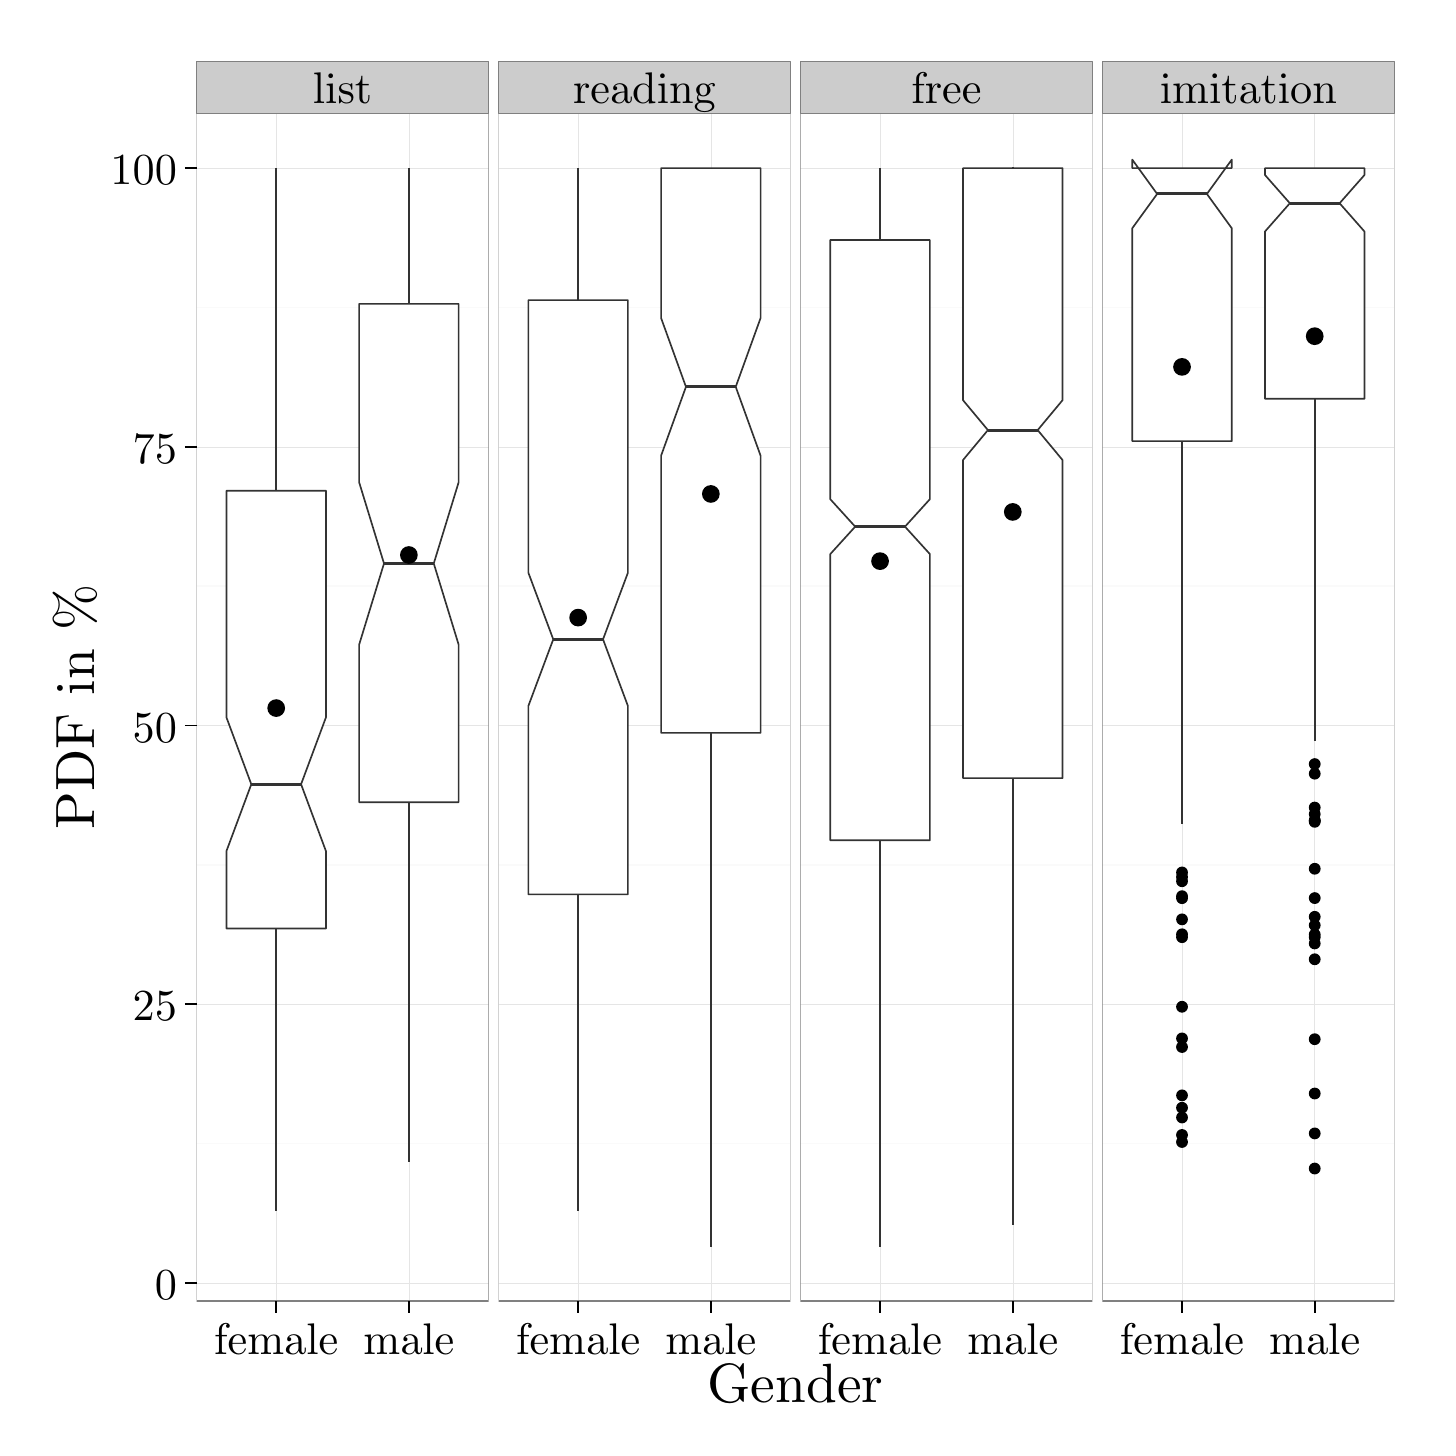
\begin{tikzpicture}[x=1pt,y=1pt]
\definecolor{fillColor}{RGB}{255,255,255}
\path[use as bounding box,fill=fillColor,fill opacity=0.00] (0,0) rectangle (505.89,505.89);
\begin{scope}
\path[clip] (  0.00,  0.00) rectangle (505.89,505.89);
\definecolor{drawColor}{RGB}{255,255,255}
\definecolor{fillColor}{RGB}{255,255,255}

\path[draw=drawColor,line width= 0.6pt,line join=round,line cap=round,fill=fillColor] (  0.00, -0.00) rectangle (505.89,505.89);
\end{scope}
\begin{scope}
\path[clip] ( 61.03, 45.77) rectangle (166.52,475.09);
\definecolor{fillColor}{RGB}{255,255,255}

\path[fill=fillColor] ( 61.03, 45.77) rectangle (166.52,475.09);
\definecolor{drawColor}{gray}{0.98}

\path[draw=drawColor,line width= 0.6pt,line join=round] ( 61.03,102.67) --
	(166.52,102.67);

\path[draw=drawColor,line width= 0.6pt,line join=round] ( 61.03,203.37) --
	(166.52,203.37);

\path[draw=drawColor,line width= 0.6pt,line join=round] ( 61.03,304.07) --
	(166.52,304.07);

\path[draw=drawColor,line width= 0.6pt,line join=round] ( 61.03,404.78) --
	(166.52,404.78);
\definecolor{drawColor}{gray}{0.90}

\path[draw=drawColor,line width= 0.2pt,line join=round] ( 61.03, 52.32) --
	(166.52, 52.32);

\path[draw=drawColor,line width= 0.2pt,line join=round] ( 61.03,153.02) --
	(166.52,153.02);

\path[draw=drawColor,line width= 0.2pt,line join=round] ( 61.03,253.72) --
	(166.52,253.72);

\path[draw=drawColor,line width= 0.2pt,line join=round] ( 61.03,354.43) --
	(166.52,354.43);

\path[draw=drawColor,line width= 0.2pt,line join=round] ( 61.03,455.13) --
	(166.52,455.13);

\path[draw=drawColor,line width= 0.2pt,line join=round] ( 89.80, 45.77) --
	( 89.80,475.09);

\path[draw=drawColor,line width= 0.2pt,line join=round] (137.75, 45.77) --
	(137.75,475.09);
\definecolor{drawColor}{gray}{0.20}

\path[draw=drawColor,line width= 0.6pt,line join=round] ( 89.80,338.56) -- ( 89.80,455.13);

\path[draw=drawColor,line width= 0.6pt,line join=round] ( 89.80,180.37) -- ( 89.80, 78.18);

\path[draw=drawColor,line width= 0.6pt,line join=round,line cap=round,fill=fillColor] ( 71.82,338.56) --
	( 71.82,256.66) --
	( 80.81,232.49) --
	( 71.82,208.33) --
	( 71.82,180.37) --
	(107.78,180.37) --
	(107.78,208.33) --
	( 98.79,232.49) --
	(107.78,256.66) --
	(107.78,338.56) --
	( 71.82,338.56) --
	cycle;

\path[draw=drawColor,line width= 1.1pt,line join=round] ( 80.81,232.49) -- ( 98.79,232.49);

\path[draw=drawColor,line width= 0.6pt,line join=round] (137.75,406.09) -- (137.75,455.13);

\path[draw=drawColor,line width= 0.6pt,line join=round] (137.75,226.02) -- (137.75, 95.82);

\path[draw=drawColor,line width= 0.6pt,line join=round,line cap=round,fill=fillColor] (119.77,406.09) --
	(119.77,341.62) --
	(128.76,312.27) --
	(119.77,282.93) --
	(119.77,226.02) --
	(155.73,226.02) --
	(155.73,282.93) --
	(146.74,312.27) --
	(155.73,341.62) --
	(155.73,406.09) --
	(119.77,406.09) --
	cycle;

\path[draw=drawColor,line width= 1.1pt,line join=round] (128.76,312.27) -- (146.74,312.27);
\definecolor{fillColor}{RGB}{0,0,0}

\path[fill=fillColor] ( 89.80,260.02) circle (  3.20);

\path[fill=fillColor] (137.75,315.34) circle (  3.20);
\definecolor{drawColor}{gray}{0.50}

\path[draw=drawColor,line width= 0.6pt,line join=round,line cap=round] ( 61.03, 45.77) rectangle (166.52,475.09);
\end{scope}
\begin{scope}
\path[clip] (170.14, 45.77) rectangle (275.63,475.09);
\definecolor{fillColor}{RGB}{255,255,255}

\path[fill=fillColor] (170.14, 45.77) rectangle (275.63,475.09);
\definecolor{drawColor}{gray}{0.98}

\path[draw=drawColor,line width= 0.6pt,line join=round] (170.14,102.67) --
	(275.63,102.67);

\path[draw=drawColor,line width= 0.6pt,line join=round] (170.14,203.37) --
	(275.63,203.37);

\path[draw=drawColor,line width= 0.6pt,line join=round] (170.14,304.07) --
	(275.63,304.07);

\path[draw=drawColor,line width= 0.6pt,line join=round] (170.14,404.78) --
	(275.63,404.78);
\definecolor{drawColor}{gray}{0.90}

\path[draw=drawColor,line width= 0.2pt,line join=round] (170.14, 52.32) --
	(275.63, 52.32);

\path[draw=drawColor,line width= 0.2pt,line join=round] (170.14,153.02) --
	(275.63,153.02);

\path[draw=drawColor,line width= 0.2pt,line join=round] (170.14,253.72) --
	(275.63,253.72);

\path[draw=drawColor,line width= 0.2pt,line join=round] (170.14,354.43) --
	(275.63,354.43);

\path[draw=drawColor,line width= 0.2pt,line join=round] (170.14,455.13) --
	(275.63,455.13);

\path[draw=drawColor,line width= 0.2pt,line join=round] (198.91, 45.77) --
	(198.91,475.09);

\path[draw=drawColor,line width= 0.2pt,line join=round] (246.86, 45.77) --
	(246.86,475.09);
\definecolor{drawColor}{gray}{0.20}

\path[draw=drawColor,line width= 0.6pt,line join=round] (198.91,407.44) -- (198.91,455.13);

\path[draw=drawColor,line width= 0.6pt,line join=round] (198.91,192.72) -- (198.91, 78.22);

\path[draw=drawColor,line width= 0.6pt,line join=round,line cap=round,fill=fillColor] (180.93,407.44) --
	(180.93,308.91) --
	(189.92,284.86) --
	(180.93,260.81) --
	(180.93,192.72) --
	(216.89,192.72) --
	(216.89,260.81) --
	(207.90,284.86) --
	(216.89,308.91) --
	(216.89,407.44) --
	(180.93,407.44) --
	cycle;

\path[draw=drawColor,line width= 1.1pt,line join=round] (189.92,284.86) -- (207.90,284.86);

\path[draw=drawColor,line width= 0.6pt,line join=round] (246.86,455.13) -- (246.86,455.13);

\path[draw=drawColor,line width= 0.6pt,line join=round] (246.86,251.06) -- (246.86, 65.45);

\path[draw=drawColor,line width= 0.6pt,line join=round,line cap=round,fill=fillColor] (228.88,455.13) --
	(228.88,400.97) --
	(237.87,376.10) --
	(228.88,351.22) --
	(228.88,251.06) --
	(264.84,251.06) --
	(264.84,351.22) --
	(255.85,376.10) --
	(264.84,400.97) --
	(264.84,455.13) --
	(228.88,455.13) --
	cycle;

\path[draw=drawColor,line width= 1.1pt,line join=round] (237.87,376.10) -- (255.85,376.10);
\definecolor{fillColor}{RGB}{0,0,0}

\path[fill=fillColor] (198.91,292.71) circle (  3.20);

\path[fill=fillColor] (246.86,337.40) circle (  3.20);
\definecolor{drawColor}{gray}{0.50}

\path[draw=drawColor,line width= 0.6pt,line join=round,line cap=round] (170.14, 45.77) rectangle (275.63,475.09);
\end{scope}
\begin{scope}
\path[clip] (279.24, 45.77) rectangle (384.74,475.09);
\definecolor{fillColor}{RGB}{255,255,255}

\path[fill=fillColor] (279.24, 45.77) rectangle (384.74,475.09);
\definecolor{drawColor}{gray}{0.98}

\path[draw=drawColor,line width= 0.6pt,line join=round] (279.24,102.67) --
	(384.74,102.67);

\path[draw=drawColor,line width= 0.6pt,line join=round] (279.24,203.37) --
	(384.74,203.37);

\path[draw=drawColor,line width= 0.6pt,line join=round] (279.24,304.07) --
	(384.74,304.07);

\path[draw=drawColor,line width= 0.6pt,line join=round] (279.24,404.78) --
	(384.74,404.78);
\definecolor{drawColor}{gray}{0.90}

\path[draw=drawColor,line width= 0.2pt,line join=round] (279.24, 52.32) --
	(384.74, 52.32);

\path[draw=drawColor,line width= 0.2pt,line join=round] (279.24,153.02) --
	(384.74,153.02);

\path[draw=drawColor,line width= 0.2pt,line join=round] (279.24,253.72) --
	(384.74,253.72);

\path[draw=drawColor,line width= 0.2pt,line join=round] (279.24,354.43) --
	(384.74,354.43);

\path[draw=drawColor,line width= 0.2pt,line join=round] (279.24,455.13) --
	(384.74,455.13);

\path[draw=drawColor,line width= 0.2pt,line join=round] (308.01, 45.77) --
	(308.01,475.09);

\path[draw=drawColor,line width= 0.2pt,line join=round] (355.97, 45.77) --
	(355.97,475.09);
\definecolor{drawColor}{gray}{0.20}

\path[draw=drawColor,line width= 0.6pt,line join=round] (308.01,429.17) -- (308.01,455.13);

\path[draw=drawColor,line width= 0.6pt,line join=round] (308.01,212.24) -- (308.01, 65.29);

\path[draw=drawColor,line width= 0.6pt,line join=round,line cap=round,fill=fillColor] (290.03,429.17) --
	(290.03,335.49) --
	(299.02,325.58) --
	(290.03,315.68) --
	(290.03,212.24) --
	(326.00,212.24) --
	(326.00,315.68) --
	(317.01,325.58) --
	(326.00,335.49) --
	(326.00,429.17) --
	(290.03,429.17) --
	cycle;

\path[draw=drawColor,line width= 1.1pt,line join=round] (299.02,325.58) -- (317.01,325.58);

\path[draw=drawColor,line width= 0.6pt,line join=round] (355.97,455.13) -- (355.97,455.57);

\path[draw=drawColor,line width= 0.6pt,line join=round] (355.97,234.71) -- (355.97, 73.10);

\path[draw=drawColor,line width= 0.6pt,line join=round,line cap=round,fill=fillColor] (337.98,455.13) --
	(337.98,371.28) --
	(346.98,360.47) --
	(337.98,349.65) --
	(337.98,234.71) --
	(373.95,234.71) --
	(373.95,349.65) --
	(364.96,360.47) --
	(373.95,371.28) --
	(373.95,455.13) --
	(337.98,455.13) --
	cycle;

\path[draw=drawColor,line width= 1.1pt,line join=round] (346.98,360.47) -- (364.96,360.47);
\definecolor{fillColor}{RGB}{0,0,0}

\path[fill=fillColor] (308.01,313.12) circle (  3.20);

\path[fill=fillColor] (355.97,330.90) circle (  3.20);
\definecolor{drawColor}{gray}{0.50}

\path[draw=drawColor,line width= 0.6pt,line join=round,line cap=round] (279.24, 45.77) rectangle (384.74,475.09);
\end{scope}
\begin{scope}
\path[clip] (388.35, 45.77) rectangle (493.84,475.09);
\definecolor{fillColor}{RGB}{255,255,255}

\path[fill=fillColor] (388.35, 45.77) rectangle (493.84,475.09);
\definecolor{drawColor}{gray}{0.98}

\path[draw=drawColor,line width= 0.6pt,line join=round] (388.35,102.67) --
	(493.84,102.67);

\path[draw=drawColor,line width= 0.6pt,line join=round] (388.35,203.37) --
	(493.84,203.37);

\path[draw=drawColor,line width= 0.6pt,line join=round] (388.35,304.07) --
	(493.84,304.07);

\path[draw=drawColor,line width= 0.6pt,line join=round] (388.35,404.78) --
	(493.84,404.78);
\definecolor{drawColor}{gray}{0.90}

\path[draw=drawColor,line width= 0.2pt,line join=round] (388.35, 52.32) --
	(493.84, 52.32);

\path[draw=drawColor,line width= 0.2pt,line join=round] (388.35,153.02) --
	(493.84,153.02);

\path[draw=drawColor,line width= 0.2pt,line join=round] (388.35,253.72) --
	(493.84,253.72);

\path[draw=drawColor,line width= 0.2pt,line join=round] (388.35,354.43) --
	(493.84,354.43);

\path[draw=drawColor,line width= 0.2pt,line join=round] (388.35,455.13) --
	(493.84,455.13);

\path[draw=drawColor,line width= 0.2pt,line join=round] (417.12, 45.77) --
	(417.12,475.09);

\path[draw=drawColor,line width= 0.2pt,line join=round] (465.07, 45.77) --
	(465.07,475.09);
\definecolor{fillColor}{RGB}{0,0,0}

\path[fill=fillColor] (417.12,115.60) circle (  2.13);

\path[fill=fillColor] (417.12,177.23) circle (  2.13);

\path[fill=fillColor] (417.12,105.77) circle (  2.13);

\path[fill=fillColor] (417.12,178.28) circle (  2.13);

\path[fill=fillColor] (417.12,120.07) circle (  2.13);

\path[fill=fillColor] (417.12,192.05) circle (  2.13);

\path[fill=fillColor] (417.12,112.09) circle (  2.13);

\path[fill=fillColor] (417.12,197.45) circle (  2.13);

\path[fill=fillColor] (417.12,152.09) circle (  2.13);

\path[fill=fillColor] (417.12,140.65) circle (  2.13);

\path[fill=fillColor] (417.12,200.63) circle (  2.13);

\path[fill=fillColor] (417.12,183.67) circle (  2.13);

\path[fill=fillColor] (417.12,191.33) circle (  2.13);

\path[fill=fillColor] (417.12,103.23) circle (  2.13);

\path[fill=fillColor] (417.12,198.98) circle (  2.13);

\path[fill=fillColor] (417.12,137.55) circle (  2.13);
\definecolor{drawColor}{gray}{0.20}

\path[draw=drawColor,line width= 0.6pt,line join=round] (417.12,455.13) -- (417.12,455.13);

\path[draw=drawColor,line width= 0.6pt,line join=round] (417.12,356.47) -- (417.12,218.23);
\definecolor{fillColor}{RGB}{255,255,255}

\path[draw=drawColor,line width= 0.6pt,line join=round,line cap=round,fill=fillColor] (399.14,455.13) --
	(399.14,458.21) --
	(408.13,445.80) --
	(399.14,433.40) --
	(399.14,356.47) --
	(435.10,356.47) --
	(435.10,433.40) --
	(426.11,445.80) --
	(435.10,458.21) --
	(435.10,455.13) --
	(399.14,455.13) --
	cycle;

\path[draw=drawColor,line width= 1.1pt,line join=round] (408.13,445.80) -- (426.11,445.80);
\definecolor{fillColor}{RGB}{0,0,0}

\path[fill=fillColor] (465.07,201.96) circle (  2.13);

\path[fill=fillColor] (465.07,140.37) circle (  2.13);

\path[fill=fillColor] (465.07, 93.64) circle (  2.13);

\path[fill=fillColor] (465.07,218.92) circle (  2.13);

\path[fill=fillColor] (465.07,221.70) circle (  2.13);

\path[fill=fillColor] (465.07,120.75) circle (  2.13);

\path[fill=fillColor] (465.07,177.23) circle (  2.13);

\path[fill=fillColor] (465.07,181.54) circle (  2.13);

\path[fill=fillColor] (465.07,239.79) circle (  2.13);

\path[fill=fillColor] (465.07,191.37) circle (  2.13);

\path[fill=fillColor] (465.07,184.60) circle (  2.13);

\path[fill=fillColor] (465.07,236.32) circle (  2.13);

\path[fill=fillColor] (465.07,219.40) circle (  2.13);

\path[fill=fillColor] (465.07,178.20) circle (  2.13);

\path[fill=fillColor] (465.07,224.08) circle (  2.13);

\path[fill=fillColor] (465.07,219.44) circle (  2.13);

\path[fill=fillColor] (465.07,106.33) circle (  2.13);

\path[fill=fillColor] (465.07,174.97) circle (  2.13);

\path[fill=fillColor] (465.07,169.25) circle (  2.13);

\path[draw=drawColor,line width= 0.6pt,line join=round] (465.07,455.13) -- (465.07,455.13);

\path[draw=drawColor,line width= 0.6pt,line join=round] (465.07,371.82) -- (465.07,248.24);
\definecolor{fillColor}{RGB}{255,255,255}

\path[draw=drawColor,line width= 0.6pt,line join=round,line cap=round,fill=fillColor] (447.09,455.13) --
	(447.09,452.66) --
	(456.08,442.44) --
	(447.09,432.22) --
	(447.09,371.82) --
	(483.06,371.82) --
	(483.06,432.22) --
	(474.06,442.44) --
	(483.06,452.66) --
	(483.06,455.13) --
	(447.09,455.13) --
	cycle;

\path[draw=drawColor,line width= 1.1pt,line join=round] (456.08,442.44) -- (474.06,442.44);
\definecolor{fillColor}{RGB}{0,0,0}

\path[fill=fillColor] (417.12,383.31) circle (  3.20);

\path[fill=fillColor] (465.07,394.40) circle (  3.20);
\definecolor{drawColor}{gray}{0.50}

\path[draw=drawColor,line width= 0.6pt,line join=round,line cap=round] (388.35, 45.77) rectangle (493.84,475.09);
\end{scope}
\begin{scope}
\path[clip] (  0.00,  0.00) rectangle (505.89,505.89);
\definecolor{drawColor}{gray}{0.50}
\definecolor{fillColor}{gray}{0.80}

\path[draw=drawColor,line width= 0.2pt,line join=round,line cap=round,fill=fillColor] ( 61.03,475.09) rectangle (166.52,493.85);
\definecolor{drawColor}{RGB}{0,0,0}

\node[text=drawColor,anchor=base,inner sep=0pt, outer sep=0pt, scale=  1.60] at (113.78,478.43) {list};
\end{scope}
\begin{scope}
\path[clip] (  0.00,  0.00) rectangle (505.89,505.89);
\definecolor{drawColor}{gray}{0.50}
\definecolor{fillColor}{gray}{0.80}

\path[draw=drawColor,line width= 0.2pt,line join=round,line cap=round,fill=fillColor] (170.14,475.09) rectangle (275.63,493.85);
\definecolor{drawColor}{RGB}{0,0,0}

\node[text=drawColor,anchor=base,inner sep=0pt, outer sep=0pt, scale=  1.60] at (222.88,478.43) {reading};
\end{scope}
\begin{scope}
\path[clip] (  0.00,  0.00) rectangle (505.89,505.89);
\definecolor{drawColor}{gray}{0.50}
\definecolor{fillColor}{gray}{0.80}

\path[draw=drawColor,line width= 0.2pt,line join=round,line cap=round,fill=fillColor] (279.24,475.09) rectangle (384.74,493.85);
\definecolor{drawColor}{RGB}{0,0,0}

\node[text=drawColor,anchor=base,inner sep=0pt, outer sep=0pt, scale=  1.60] at (331.99,478.43) {free};
\end{scope}
\begin{scope}
\path[clip] (  0.00,  0.00) rectangle (505.89,505.89);
\definecolor{drawColor}{gray}{0.50}
\definecolor{fillColor}{gray}{0.80}

\path[draw=drawColor,line width= 0.2pt,line join=round,line cap=round,fill=fillColor] (388.35,475.09) rectangle (493.84,493.85);
\definecolor{drawColor}{RGB}{0,0,0}

\node[text=drawColor,anchor=base,inner sep=0pt, outer sep=0pt, scale=  1.60] at (441.10,478.43) {imitation};
\end{scope}
\begin{scope}
\path[clip] (  0.00,  0.00) rectangle (505.89,505.89);
\definecolor{drawColor}{RGB}{0,0,0}

\node[text=drawColor,anchor=base east,inner sep=0pt, outer sep=0pt, scale=  1.60] at ( 53.92, 46.28) {0};

\node[text=drawColor,anchor=base east,inner sep=0pt, outer sep=0pt, scale=  1.60] at ( 53.92,146.99) {25};

\node[text=drawColor,anchor=base east,inner sep=0pt, outer sep=0pt, scale=  1.60] at ( 53.92,247.69) {50};

\node[text=drawColor,anchor=base east,inner sep=0pt, outer sep=0pt, scale=  1.60] at ( 53.92,348.39) {75};

\node[text=drawColor,anchor=base east,inner sep=0pt, outer sep=0pt, scale=  1.60] at ( 53.92,449.10) {100};
\end{scope}
\begin{scope}
\path[clip] (  0.00,  0.00) rectangle (505.89,505.89);
\definecolor{drawColor}{RGB}{0,0,0}

\path[draw=drawColor,line width= 0.6pt,line join=round] ( 56.76, 52.32) --
	( 61.03, 52.32);

\path[draw=drawColor,line width= 0.6pt,line join=round] ( 56.76,153.02) --
	( 61.03,153.02);

\path[draw=drawColor,line width= 0.6pt,line join=round] ( 56.76,253.72) --
	( 61.03,253.72);

\path[draw=drawColor,line width= 0.6pt,line join=round] ( 56.76,354.43) --
	( 61.03,354.43);

\path[draw=drawColor,line width= 0.6pt,line join=round] ( 56.76,455.13) --
	( 61.03,455.13);
\end{scope}
\begin{scope}
\path[clip] (  0.00,  0.00) rectangle (505.89,505.89);
\definecolor{drawColor}{RGB}{0,0,0}

\path[draw=drawColor,line width= 0.6pt,line join=round] ( 89.80, 41.50) --
	( 89.80, 45.77);

\path[draw=drawColor,line width= 0.6pt,line join=round] (137.75, 41.50) --
	(137.75, 45.77);
\end{scope}
\begin{scope}
\path[clip] (  0.00,  0.00) rectangle (505.89,505.89);
\definecolor{drawColor}{RGB}{0,0,0}

\node[text=drawColor,anchor=base,inner sep=0pt, outer sep=0pt, scale=  1.60] at ( 89.80, 26.59) {female};

\node[text=drawColor,anchor=base,inner sep=0pt, outer sep=0pt, scale=  1.60] at (137.75, 26.59) {male};
\end{scope}
\begin{scope}
\path[clip] (  0.00,  0.00) rectangle (505.89,505.89);
\definecolor{drawColor}{RGB}{0,0,0}

\path[draw=drawColor,line width= 0.6pt,line join=round] (198.91, 41.50) --
	(198.91, 45.77);

\path[draw=drawColor,line width= 0.6pt,line join=round] (246.86, 41.50) --
	(246.86, 45.77);
\end{scope}
\begin{scope}
\path[clip] (  0.00,  0.00) rectangle (505.89,505.89);
\definecolor{drawColor}{RGB}{0,0,0}

\node[text=drawColor,anchor=base,inner sep=0pt, outer sep=0pt, scale=  1.60] at (198.91, 26.59) {female};

\node[text=drawColor,anchor=base,inner sep=0pt, outer sep=0pt, scale=  1.60] at (246.86, 26.59) {male};
\end{scope}
\begin{scope}
\path[clip] (  0.00,  0.00) rectangle (505.89,505.89);
\definecolor{drawColor}{RGB}{0,0,0}

\path[draw=drawColor,line width= 0.6pt,line join=round] (308.01, 41.50) --
	(308.01, 45.77);

\path[draw=drawColor,line width= 0.6pt,line join=round] (355.97, 41.50) --
	(355.97, 45.77);
\end{scope}
\begin{scope}
\path[clip] (  0.00,  0.00) rectangle (505.89,505.89);
\definecolor{drawColor}{RGB}{0,0,0}

\node[text=drawColor,anchor=base,inner sep=0pt, outer sep=0pt, scale=  1.60] at (308.01, 26.59) {female};

\node[text=drawColor,anchor=base,inner sep=0pt, outer sep=0pt, scale=  1.60] at (355.97, 26.59) {male};
\end{scope}
\begin{scope}
\path[clip] (  0.00,  0.00) rectangle (505.89,505.89);
\definecolor{drawColor}{RGB}{0,0,0}

\path[draw=drawColor,line width= 0.6pt,line join=round] (417.12, 41.50) --
	(417.12, 45.77);

\path[draw=drawColor,line width= 0.6pt,line join=round] (465.07, 41.50) --
	(465.07, 45.77);
\end{scope}
\begin{scope}
\path[clip] (  0.00,  0.00) rectangle (505.89,505.89);
\definecolor{drawColor}{RGB}{0,0,0}

\node[text=drawColor,anchor=base,inner sep=0pt, outer sep=0pt, scale=  1.60] at (417.12, 26.59) {female};

\node[text=drawColor,anchor=base,inner sep=0pt, outer sep=0pt, scale=  1.60] at (465.07, 26.59) {male};
\end{scope}
\begin{scope}
\path[clip] (  0.00,  0.00) rectangle (505.89,505.89);
\definecolor{drawColor}{RGB}{0,0,0}

\node[text=drawColor,anchor=base,inner sep=0pt, outer sep=0pt, scale=  2.00] at (277.44,  9.03) {Gender};
\end{scope}
\begin{scope}
\path[clip] (  0.00,  0.00) rectangle (505.89,505.89);
\definecolor{drawColor}{RGB}{0,0,0}

\node[text=drawColor,rotate= 90.00,anchor=base,inner sep=0pt, outer sep=0pt, scale=  2.00] at ( 24.12,260.43) {PDF in {\%}};
\end{scope}
\end{tikzpicture}
} 
	\caption{/k/: PDF by style and gender (released only)}
	\label{fig.box.k.stylegender}
\end{figure}

We will start the analysis of social predictors by looking at the interaction of gender and style, which is visualised by \figref{fig.box.k.stylegender}.
One thing that can be gleaned from the box plots is that there is a substantial amount of variation when it comes to the realisation of /k/.
With the exception of accent imitation\is{accent performance} (in the rightmost panel), all boxes have a relatively large vertical extent.
As the lower and upper bounds of the boxes mark the first and third quantiles, respectively, large boxes indicate that there is a comparatively large spread of data around the mean.
In the case at hand, this means that a wide range of realisations can be found in sizeable numbers (and not just as individual outliers) in the recordings, going from more standard variants (with \isi{PDF}s of around 30) to clearly Scouse pronunciations (with \isi{PDF}s of 75+).
This large amount of variation seems to be characteristic of /k/ realisations in my sample: it was already present in \figref{fig.box.k.environment}, and it will be visible in most of the other graphs that will follow in the remainder of this section.

When we look at the gender difference in the three styles word list, reading passage, and spontaneous speech (first three panels from the left in \figref{fig.box.k.stylegender}), a very clear (and expected) pattern emerges: women have lower \isi{PDF} values than men, i.e. they use less (or fewer) lenited variants of /k/.
The notches in the graph (no overlap) suggest that the medians of women and men are significantly different in all three styles, and t-tests confirm that the same is true for the means.
There is thus a statistically robust gender difference for the word list (t(198.97) = -3.554, p < 0.001), the reading passage (t(360.608) = -3.589, p < 0.001), and free speech (t(2201.103) = -3.594, p < 0.001).
When subjects are asked to put on a particularly strong Scouse accent, however, /k/ realisations of women and men are no longer significantly different from one another (t(312.112) = -1.044, p = 0.297).
Both genders use strongly lenited variants with \isi{PDF}s of 75 and higher more than 75\% of the time (cf. the position of the first quantiles in the rightmost panel of \figref{fig.box.k.stylegender}).

\begin{table}[h]
	\centering
	\caption{/k/: t-tests of style by gender}
	\label{tab.k.genderstyle.pvalues}
	\begin{tabular}{lrrrrrr}
		\toprule
		test & \multicolumn{3}{c}{women} & \multicolumn{3}{c}{men}\\
		& t & df & p & t & df & p\\
		\midrule
		list-reading & \ensuremath{-2.293} & 226.274 & 0.023 & \ensuremath{-1.583} & 210.281 & 0.115\\
		list-free & \ensuremath{-4.500} & 126.152 & < 0.001 & \ensuremath{-1.378} & 114.832 & 0.171\\
		list-imitation\is{accent performance} & \ensuremath{-8.881} & 205.652 & < 0.001 & \ensuremath{-6.201} & 170.062 & < 0.001\\
		reading-free & \ensuremath{-2.186} & 262.723 & 0.030 & 0.676 & 224.321 & 0.500\\
		reading-imitation\is{accent performance} & \ensuremath{-7.637} & 354.391 & < 0.001 & \ensuremath{-5.052} & 313.565 & < 0.001\\
		free-imitation\is{accent performance} & \ensuremath{-8.009} & 217.296 & < 0.001 & \ensuremath{-8.152} & 262.352 & < 0.001\\
		\bottomrule
	\end{tabular}
\end{table}

If we focus on the style dimension within the two gender subgroups separately, differences emerge as well.
The graph shows that accent imitation\is{accent performance} is clearly separate from the other three styles (the means are much higher than in any of the other registers).
This holds true for both women and men, but when the analysis is restricted to female speakers, the styles word list, reading passage, and free speech are also distinguishable from each other.
Medians seem to be distinct, and t-tests on the raw data (cf. \tabref{tab.k.genderstyle.pvalues}) show that the differences in means are also statistically robust.
For men, on the other hand, means are closer together and there is some overlap between the confidence intervals of the medians as well.
T-tests confirm that men have statistically identical /k/ realisations in free speech, the reading, and the word list task; only accent perform\is{accent performance}ance is significantly different from these three (cf. again \tabref{tab.k.genderstyle.pvalues}).
In my sample, style is therefore less important for men than it is for women.

\subsection{Style and social class}
\label{sec.prod.res.con.k.styleclass}

\begin{figure}[h]
	\centering
		\definecolor{shadecolor}{rgb}{0.969, 0.969, 0.969}
		\resizebox{0.49\linewidth}{!}{% Created by tikzDevice version 0.8.1 on 2016-02-09 02:17:20
% !TEX encoding = UTF-8 Unicode
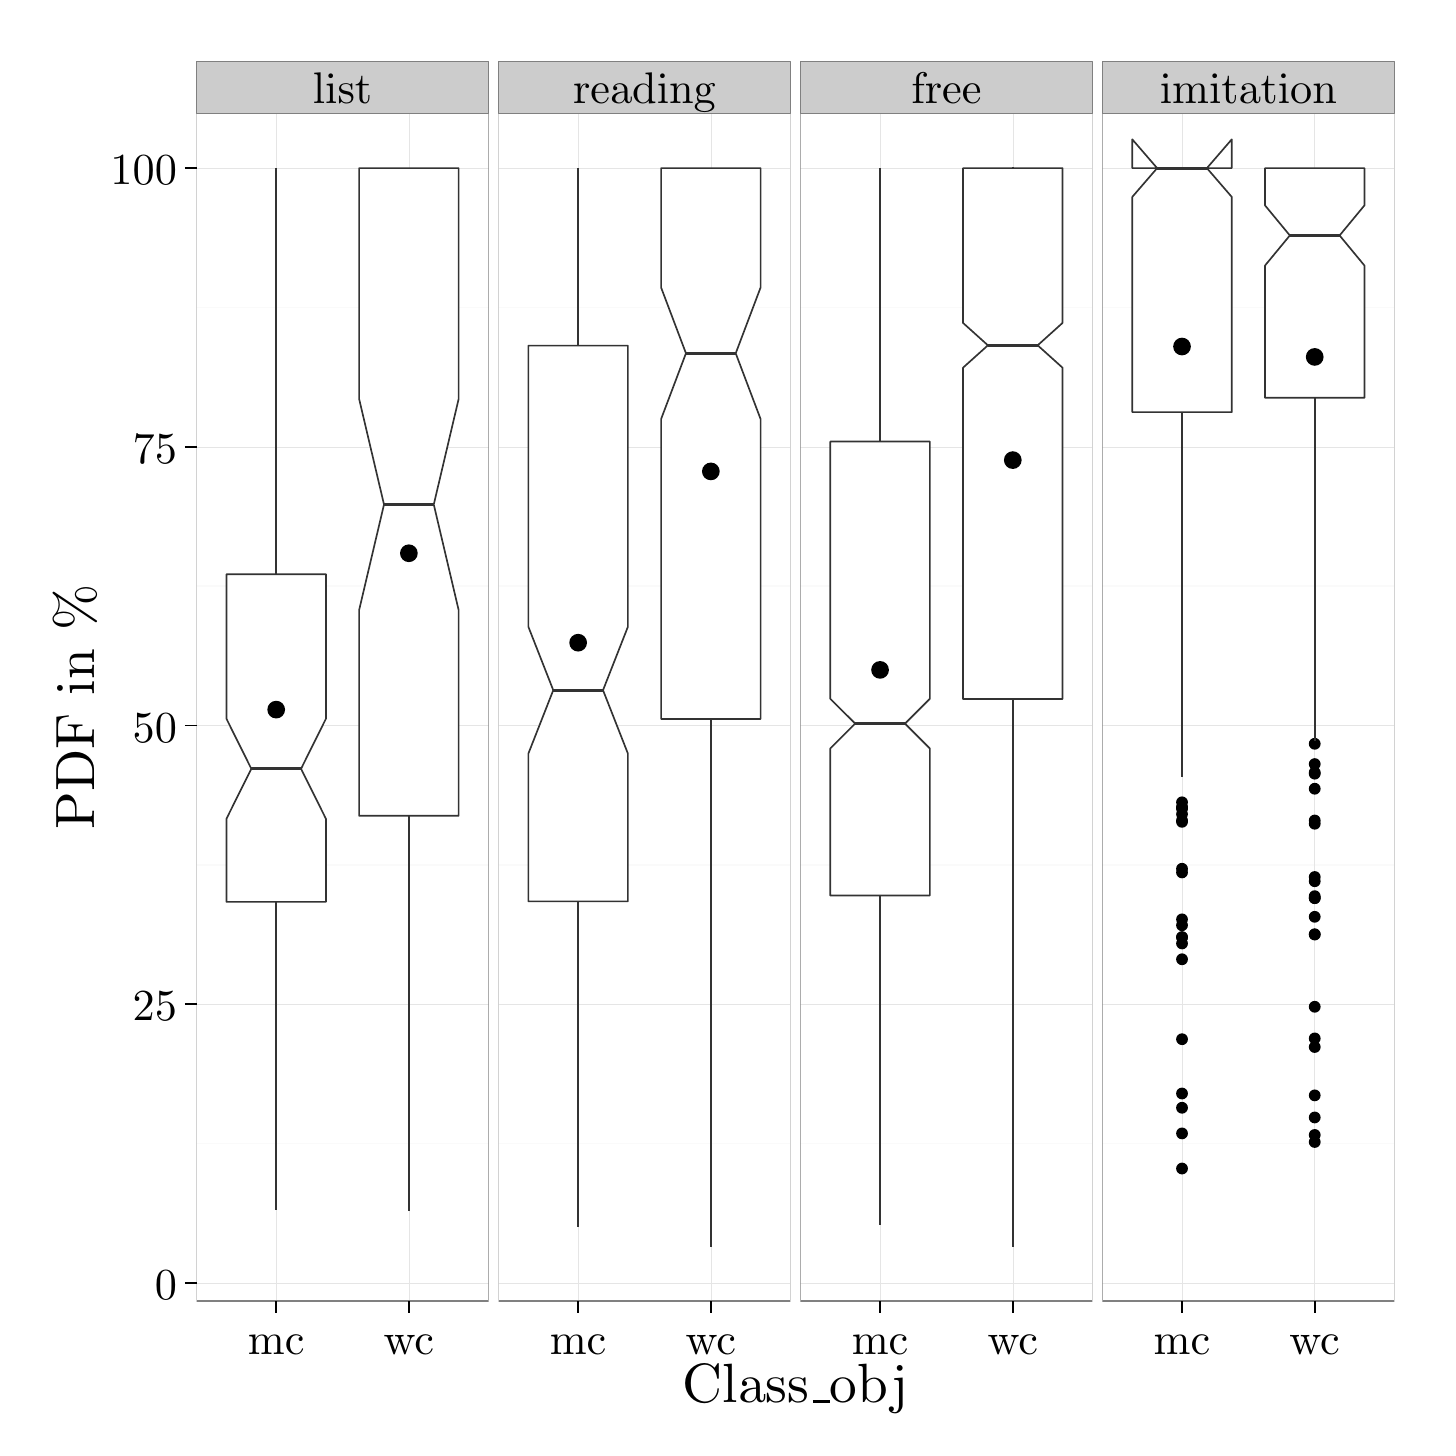
\begin{tikzpicture}[x=1pt,y=1pt]
\definecolor{fillColor}{RGB}{255,255,255}
\path[use as bounding box,fill=fillColor,fill opacity=0.00] (0,0) rectangle (505.89,505.89);
\begin{scope}
\path[clip] (  0.00,  0.00) rectangle (505.89,505.89);
\definecolor{drawColor}{RGB}{255,255,255}
\definecolor{fillColor}{RGB}{255,255,255}

\path[draw=drawColor,line width= 0.6pt,line join=round,line cap=round,fill=fillColor] (  0.00, -0.00) rectangle (505.89,505.89);
\end{scope}
\begin{scope}
\path[clip] ( 61.03, 45.77) rectangle (166.52,475.09);
\definecolor{fillColor}{RGB}{255,255,255}

\path[fill=fillColor] ( 61.03, 45.77) rectangle (166.52,475.09);
\definecolor{drawColor}{gray}{0.98}

\path[draw=drawColor,line width= 0.6pt,line join=round] ( 61.03,102.67) --
	(166.52,102.67);

\path[draw=drawColor,line width= 0.6pt,line join=round] ( 61.03,203.37) --
	(166.52,203.37);

\path[draw=drawColor,line width= 0.6pt,line join=round] ( 61.03,304.07) --
	(166.52,304.07);

\path[draw=drawColor,line width= 0.6pt,line join=round] ( 61.03,404.78) --
	(166.52,404.78);
\definecolor{drawColor}{gray}{0.90}

\path[draw=drawColor,line width= 0.2pt,line join=round] ( 61.03, 52.32) --
	(166.52, 52.32);

\path[draw=drawColor,line width= 0.2pt,line join=round] ( 61.03,153.02) --
	(166.52,153.02);

\path[draw=drawColor,line width= 0.2pt,line join=round] ( 61.03,253.72) --
	(166.52,253.72);

\path[draw=drawColor,line width= 0.2pt,line join=round] ( 61.03,354.43) --
	(166.52,354.43);

\path[draw=drawColor,line width= 0.2pt,line join=round] ( 61.03,455.13) --
	(166.52,455.13);

\path[draw=drawColor,line width= 0.2pt,line join=round] ( 89.80, 45.77) --
	( 89.80,475.09);

\path[draw=drawColor,line width= 0.2pt,line join=round] (137.75, 45.77) --
	(137.75,475.09);
\definecolor{drawColor}{gray}{0.20}

\path[draw=drawColor,line width= 0.6pt,line join=round] ( 89.80,308.38) -- ( 89.80,455.13);

\path[draw=drawColor,line width= 0.6pt,line join=round] ( 89.80,189.98) -- ( 89.80, 78.74);

\path[draw=drawColor,line width= 0.6pt,line join=round,line cap=round,fill=fillColor] ( 71.82,308.38) --
	( 71.82,256.18) --
	( 80.81,238.09) --
	( 71.82,220.01) --
	( 71.82,189.98) --
	(107.78,189.98) --
	(107.78,220.01) --
	( 98.79,238.09) --
	(107.78,256.18) --
	(107.78,308.38) --
	( 71.82,308.38) --
	cycle;

\path[draw=drawColor,line width= 1.1pt,line join=round] ( 80.81,238.09) -- ( 98.79,238.09);

\path[draw=drawColor,line width= 0.6pt,line join=round] (137.75,455.13) -- (137.75,455.13);

\path[draw=drawColor,line width= 0.6pt,line join=round] (137.75,221.09) -- (137.75, 78.18);

\path[draw=drawColor,line width= 0.6pt,line join=round,line cap=round,fill=fillColor] (119.77,455.13) --
	(119.77,371.72) --
	(128.76,333.58) --
	(119.77,295.44) --
	(119.77,221.09) --
	(155.73,221.09) --
	(155.73,295.44) --
	(146.74,333.58) --
	(155.73,371.72) --
	(155.73,455.13) --
	(119.77,455.13) --
	cycle;

\path[draw=drawColor,line width= 1.1pt,line join=round] (128.76,333.58) -- (146.74,333.58);
\definecolor{fillColor}{RGB}{0,0,0}

\path[fill=fillColor] ( 89.80,259.46) circle (  3.20);

\path[fill=fillColor] (137.75,315.97) circle (  3.20);
\definecolor{drawColor}{gray}{0.50}

\path[draw=drawColor,line width= 0.6pt,line join=round,line cap=round] ( 61.03, 45.77) rectangle (166.52,475.09);
\end{scope}
\begin{scope}
\path[clip] (170.14, 45.77) rectangle (275.63,475.09);
\definecolor{fillColor}{RGB}{255,255,255}

\path[fill=fillColor] (170.14, 45.77) rectangle (275.63,475.09);
\definecolor{drawColor}{gray}{0.98}

\path[draw=drawColor,line width= 0.6pt,line join=round] (170.14,102.67) --
	(275.63,102.67);

\path[draw=drawColor,line width= 0.6pt,line join=round] (170.14,203.37) --
	(275.63,203.37);

\path[draw=drawColor,line width= 0.6pt,line join=round] (170.14,304.07) --
	(275.63,304.07);

\path[draw=drawColor,line width= 0.6pt,line join=round] (170.14,404.78) --
	(275.63,404.78);
\definecolor{drawColor}{gray}{0.90}

\path[draw=drawColor,line width= 0.2pt,line join=round] (170.14, 52.32) --
	(275.63, 52.32);

\path[draw=drawColor,line width= 0.2pt,line join=round] (170.14,153.02) --
	(275.63,153.02);

\path[draw=drawColor,line width= 0.2pt,line join=round] (170.14,253.72) --
	(275.63,253.72);

\path[draw=drawColor,line width= 0.2pt,line join=round] (170.14,354.43) --
	(275.63,354.43);

\path[draw=drawColor,line width= 0.2pt,line join=round] (170.14,455.13) --
	(275.63,455.13);

\path[draw=drawColor,line width= 0.2pt,line join=round] (198.91, 45.77) --
	(198.91,475.09);

\path[draw=drawColor,line width= 0.2pt,line join=round] (246.86, 45.77) --
	(246.86,475.09);
\definecolor{drawColor}{gray}{0.20}

\path[draw=drawColor,line width= 0.6pt,line join=round] (198.91,390.98) -- (198.91,455.13);

\path[draw=drawColor,line width= 0.6pt,line join=round] (198.91,190.17) -- (198.91, 72.66);

\path[draw=drawColor,line width= 0.6pt,line join=round,line cap=round,fill=fillColor] (180.93,390.98) --
	(180.93,289.39) --
	(189.92,266.49) --
	(180.93,243.59) --
	(180.93,190.17) --
	(216.89,190.17) --
	(216.89,243.59) --
	(207.90,266.49) --
	(216.89,289.39) --
	(216.89,390.98) --
	(180.93,390.98) --
	cycle;

\path[draw=drawColor,line width= 1.1pt,line join=round] (189.92,266.49) -- (207.90,266.49);

\path[draw=drawColor,line width= 0.6pt,line join=round] (246.86,455.13) -- (246.86,455.13);

\path[draw=drawColor,line width= 0.6pt,line join=round] (246.86,256.08) -- (246.86, 65.45);

\path[draw=drawColor,line width= 0.6pt,line join=round,line cap=round,fill=fillColor] (228.88,455.13) --
	(228.88,412.00) --
	(237.87,388.22) --
	(228.88,364.45) --
	(228.88,256.08) --
	(264.84,256.08) --
	(264.84,364.45) --
	(255.85,388.22) --
	(264.84,412.00) --
	(264.84,455.13) --
	(228.88,455.13) --
	cycle;

\path[draw=drawColor,line width= 1.1pt,line join=round] (237.87,388.22) -- (255.85,388.22);
\definecolor{fillColor}{RGB}{0,0,0}

\path[fill=fillColor] (198.91,283.65) circle (  3.20);

\path[fill=fillColor] (246.86,345.54) circle (  3.20);
\definecolor{drawColor}{gray}{0.50}

\path[draw=drawColor,line width= 0.6pt,line join=round,line cap=round] (170.14, 45.77) rectangle (275.63,475.09);
\end{scope}
\begin{scope}
\path[clip] (279.24, 45.77) rectangle (384.74,475.09);
\definecolor{fillColor}{RGB}{255,255,255}

\path[fill=fillColor] (279.24, 45.77) rectangle (384.74,475.09);
\definecolor{drawColor}{gray}{0.98}

\path[draw=drawColor,line width= 0.6pt,line join=round] (279.24,102.67) --
	(384.74,102.67);

\path[draw=drawColor,line width= 0.6pt,line join=round] (279.24,203.37) --
	(384.74,203.37);

\path[draw=drawColor,line width= 0.6pt,line join=round] (279.24,304.07) --
	(384.74,304.07);

\path[draw=drawColor,line width= 0.6pt,line join=round] (279.24,404.78) --
	(384.74,404.78);
\definecolor{drawColor}{gray}{0.90}

\path[draw=drawColor,line width= 0.2pt,line join=round] (279.24, 52.32) --
	(384.74, 52.32);

\path[draw=drawColor,line width= 0.2pt,line join=round] (279.24,153.02) --
	(384.74,153.02);

\path[draw=drawColor,line width= 0.2pt,line join=round] (279.24,253.72) --
	(384.74,253.72);

\path[draw=drawColor,line width= 0.2pt,line join=round] (279.24,354.43) --
	(384.74,354.43);

\path[draw=drawColor,line width= 0.2pt,line join=round] (279.24,455.13) --
	(384.74,455.13);

\path[draw=drawColor,line width= 0.2pt,line join=round] (308.01, 45.77) --
	(308.01,475.09);

\path[draw=drawColor,line width= 0.2pt,line join=round] (355.97, 45.77) --
	(355.97,475.09);
\definecolor{drawColor}{gray}{0.20}

\path[draw=drawColor,line width= 0.6pt,line join=round] (308.01,356.32) -- (308.01,455.13);

\path[draw=drawColor,line width= 0.6pt,line join=round] (308.01,192.29) -- (308.01, 73.10);

\path[draw=drawColor,line width= 0.6pt,line join=round,line cap=round,fill=fillColor] (290.03,356.32) --
	(290.03,263.39) --
	(299.02,254.41) --
	(290.03,245.43) --
	(290.03,192.29) --
	(326.00,192.29) --
	(326.00,245.43) --
	(317.01,254.41) --
	(326.00,263.39) --
	(326.00,356.32) --
	(290.03,356.32) --
	cycle;

\path[draw=drawColor,line width= 1.1pt,line join=round] (299.02,254.41) -- (317.01,254.41);

\path[draw=drawColor,line width= 0.6pt,line join=round] (355.97,455.13) -- (355.97,455.57);

\path[draw=drawColor,line width= 0.6pt,line join=round] (355.97,263.31) -- (355.97, 65.29);

\path[draw=drawColor,line width= 0.6pt,line join=round,line cap=round,fill=fillColor] (337.98,455.13) --
	(337.98,399.20) --
	(346.98,391.10) --
	(337.98,383.01) --
	(337.98,263.31) --
	(373.95,263.31) --
	(373.95,383.01) --
	(364.96,391.10) --
	(373.95,399.20) --
	(373.95,455.13) --
	(337.98,455.13) --
	cycle;

\path[draw=drawColor,line width= 1.1pt,line join=round] (346.98,391.10) -- (364.96,391.10);
\definecolor{fillColor}{RGB}{0,0,0}

\path[fill=fillColor] (308.01,273.82) circle (  3.20);

\path[fill=fillColor] (355.97,349.63) circle (  3.20);
\definecolor{drawColor}{gray}{0.50}

\path[draw=drawColor,line width= 0.6pt,line join=round,line cap=round] (279.24, 45.77) rectangle (384.74,475.09);
\end{scope}
\begin{scope}
\path[clip] (388.35, 45.77) rectangle (493.84,475.09);
\definecolor{fillColor}{RGB}{255,255,255}

\path[fill=fillColor] (388.35, 45.77) rectangle (493.84,475.09);
\definecolor{drawColor}{gray}{0.98}

\path[draw=drawColor,line width= 0.6pt,line join=round] (388.35,102.67) --
	(493.84,102.67);

\path[draw=drawColor,line width= 0.6pt,line join=round] (388.35,203.37) --
	(493.84,203.37);

\path[draw=drawColor,line width= 0.6pt,line join=round] (388.35,304.07) --
	(493.84,304.07);

\path[draw=drawColor,line width= 0.6pt,line join=round] (388.35,404.78) --
	(493.84,404.78);
\definecolor{drawColor}{gray}{0.90}

\path[draw=drawColor,line width= 0.2pt,line join=round] (388.35, 52.32) --
	(493.84, 52.32);

\path[draw=drawColor,line width= 0.2pt,line join=round] (388.35,153.02) --
	(493.84,153.02);

\path[draw=drawColor,line width= 0.2pt,line join=round] (388.35,253.72) --
	(493.84,253.72);

\path[draw=drawColor,line width= 0.2pt,line join=round] (388.35,354.43) --
	(493.84,354.43);

\path[draw=drawColor,line width= 0.2pt,line join=round] (388.35,455.13) --
	(493.84,455.13);

\path[draw=drawColor,line width= 0.2pt,line join=round] (417.12, 45.77) --
	(417.12,475.09);

\path[draw=drawColor,line width= 0.2pt,line join=round] (465.07, 45.77) --
	(465.07,475.09);
\definecolor{fillColor}{RGB}{0,0,0}

\path[fill=fillColor] (417.12,201.96) circle (  2.13);

\path[fill=fillColor] (417.12,140.37) circle (  2.13);

\path[fill=fillColor] (417.12, 93.64) circle (  2.13);

\path[fill=fillColor] (417.12,218.92) circle (  2.13);

\path[fill=fillColor] (417.12,221.70) circle (  2.13);

\path[fill=fillColor] (417.12,120.75) circle (  2.13);

\path[fill=fillColor] (417.12,177.23) circle (  2.13);

\path[fill=fillColor] (417.12,181.54) circle (  2.13);

\path[fill=fillColor] (417.12,223.71) circle (  2.13);

\path[fill=fillColor] (417.12,115.60) circle (  2.13);

\path[fill=fillColor] (417.12,177.23) circle (  2.13);

\path[fill=fillColor] (417.12,225.97) circle (  2.13);

\path[fill=fillColor] (417.12,224.08) circle (  2.13);

\path[fill=fillColor] (417.12,219.44) circle (  2.13);

\path[fill=fillColor] (417.12,106.33) circle (  2.13);

\path[fill=fillColor] (417.12,174.97) circle (  2.13);

\path[fill=fillColor] (417.12,169.25) circle (  2.13);

\path[fill=fillColor] (417.12,224.08) circle (  2.13);

\path[fill=fillColor] (417.12,200.63) circle (  2.13);

\path[fill=fillColor] (417.12,183.67) circle (  2.13);
\definecolor{drawColor}{gray}{0.20}

\path[draw=drawColor,line width= 0.6pt,line join=round] (417.12,455.13) -- (417.12,455.13);

\path[draw=drawColor,line width= 0.6pt,line join=round] (417.12,366.95) -- (417.12,235.07);
\definecolor{fillColor}{RGB}{255,255,255}

\path[draw=drawColor,line width= 0.6pt,line join=round,line cap=round,fill=fillColor] (399.14,455.13) --
	(399.14,465.54) --
	(408.13,455.13) --
	(399.14,444.72) --
	(399.14,366.95) --
	(435.10,366.95) --
	(435.10,444.72) --
	(426.11,455.13) --
	(435.10,465.54) --
	(435.10,455.13) --
	(399.14,455.13) --
	cycle;

\path[draw=drawColor,line width= 1.1pt,line join=round] (408.13,455.13) -- (426.11,455.13);
\definecolor{fillColor}{RGB}{0,0,0}

\path[fill=fillColor] (465.07,239.79) circle (  2.13);

\path[fill=fillColor] (465.07,191.37) circle (  2.13);

\path[fill=fillColor] (465.07,184.60) circle (  2.13);

\path[fill=fillColor] (465.07,236.32) circle (  2.13);

\path[fill=fillColor] (465.07,219.40) circle (  2.13);

\path[fill=fillColor] (465.07,178.20) circle (  2.13);

\path[fill=fillColor] (465.07,105.77) circle (  2.13);

\path[fill=fillColor] (465.07,178.28) circle (  2.13);

\path[fill=fillColor] (465.07,120.07) circle (  2.13);

\path[fill=fillColor] (465.07,218.23) circle (  2.13);

\path[fill=fillColor] (465.07,192.05) circle (  2.13);

\path[fill=fillColor] (465.07,236.76) circle (  2.13);

\path[fill=fillColor] (465.07,112.09) circle (  2.13);

\path[fill=fillColor] (465.07,197.45) circle (  2.13);

\path[fill=fillColor] (465.07,152.09) circle (  2.13);

\path[fill=fillColor] (465.07,140.65) circle (  2.13);

\path[fill=fillColor] (465.07,191.33) circle (  2.13);

\path[fill=fillColor] (465.07,230.88) circle (  2.13);

\path[fill=fillColor] (465.07,247.12) circle (  2.13);

\path[fill=fillColor] (465.07,103.23) circle (  2.13);

\path[fill=fillColor] (465.07,198.98) circle (  2.13);

\path[fill=fillColor] (465.07,137.55) circle (  2.13);

\path[draw=drawColor,line width= 0.6pt,line join=round] (465.07,455.13) -- (465.07,455.13);

\path[draw=drawColor,line width= 0.6pt,line join=round] (465.07,372.15) -- (465.07,248.24);
\definecolor{fillColor}{RGB}{255,255,255}

\path[draw=drawColor,line width= 0.6pt,line join=round,line cap=round,fill=fillColor] (447.09,455.13) --
	(447.09,441.69) --
	(456.08,430.80) --
	(447.09,419.91) --
	(447.09,372.15) --
	(483.06,372.15) --
	(483.06,419.91) --
	(474.06,430.80) --
	(483.06,441.69) --
	(483.06,455.13) --
	(447.09,455.13) --
	cycle;

\path[draw=drawColor,line width= 1.1pt,line join=round] (456.08,430.80) -- (474.06,430.80);
\definecolor{fillColor}{RGB}{0,0,0}

\path[fill=fillColor] (417.12,390.67) circle (  3.20);

\path[fill=fillColor] (465.07,386.91) circle (  3.20);
\definecolor{drawColor}{gray}{0.50}

\path[draw=drawColor,line width= 0.6pt,line join=round,line cap=round] (388.35, 45.77) rectangle (493.84,475.09);
\end{scope}
\begin{scope}
\path[clip] (  0.00,  0.00) rectangle (505.89,505.89);
\definecolor{drawColor}{gray}{0.50}
\definecolor{fillColor}{gray}{0.80}

\path[draw=drawColor,line width= 0.2pt,line join=round,line cap=round,fill=fillColor] ( 61.03,475.09) rectangle (166.52,493.85);
\definecolor{drawColor}{RGB}{0,0,0}

\node[text=drawColor,anchor=base,inner sep=0pt, outer sep=0pt, scale=  1.60] at (113.78,478.43) {list};
\end{scope}
\begin{scope}
\path[clip] (  0.00,  0.00) rectangle (505.89,505.89);
\definecolor{drawColor}{gray}{0.50}
\definecolor{fillColor}{gray}{0.80}

\path[draw=drawColor,line width= 0.2pt,line join=round,line cap=round,fill=fillColor] (170.14,475.09) rectangle (275.63,493.85);
\definecolor{drawColor}{RGB}{0,0,0}

\node[text=drawColor,anchor=base,inner sep=0pt, outer sep=0pt, scale=  1.60] at (222.88,478.43) {reading};
\end{scope}
\begin{scope}
\path[clip] (  0.00,  0.00) rectangle (505.89,505.89);
\definecolor{drawColor}{gray}{0.50}
\definecolor{fillColor}{gray}{0.80}

\path[draw=drawColor,line width= 0.2pt,line join=round,line cap=round,fill=fillColor] (279.24,475.09) rectangle (384.74,493.85);
\definecolor{drawColor}{RGB}{0,0,0}

\node[text=drawColor,anchor=base,inner sep=0pt, outer sep=0pt, scale=  1.60] at (331.99,478.43) {free};
\end{scope}
\begin{scope}
\path[clip] (  0.00,  0.00) rectangle (505.89,505.89);
\definecolor{drawColor}{gray}{0.50}
\definecolor{fillColor}{gray}{0.80}

\path[draw=drawColor,line width= 0.2pt,line join=round,line cap=round,fill=fillColor] (388.35,475.09) rectangle (493.84,493.85);
\definecolor{drawColor}{RGB}{0,0,0}

\node[text=drawColor,anchor=base,inner sep=0pt, outer sep=0pt, scale=  1.60] at (441.10,478.43) {imitation};
\end{scope}
\begin{scope}
\path[clip] (  0.00,  0.00) rectangle (505.89,505.89);
\definecolor{drawColor}{RGB}{0,0,0}

\node[text=drawColor,anchor=base east,inner sep=0pt, outer sep=0pt, scale=  1.60] at ( 53.92, 46.28) {0};

\node[text=drawColor,anchor=base east,inner sep=0pt, outer sep=0pt, scale=  1.60] at ( 53.92,146.99) {25};

\node[text=drawColor,anchor=base east,inner sep=0pt, outer sep=0pt, scale=  1.60] at ( 53.92,247.69) {50};

\node[text=drawColor,anchor=base east,inner sep=0pt, outer sep=0pt, scale=  1.60] at ( 53.92,348.39) {75};

\node[text=drawColor,anchor=base east,inner sep=0pt, outer sep=0pt, scale=  1.60] at ( 53.92,449.10) {100};
\end{scope}
\begin{scope}
\path[clip] (  0.00,  0.00) rectangle (505.89,505.89);
\definecolor{drawColor}{RGB}{0,0,0}

\path[draw=drawColor,line width= 0.6pt,line join=round] ( 56.76, 52.32) --
	( 61.03, 52.32);

\path[draw=drawColor,line width= 0.6pt,line join=round] ( 56.76,153.02) --
	( 61.03,153.02);

\path[draw=drawColor,line width= 0.6pt,line join=round] ( 56.76,253.72) --
	( 61.03,253.72);

\path[draw=drawColor,line width= 0.6pt,line join=round] ( 56.76,354.43) --
	( 61.03,354.43);

\path[draw=drawColor,line width= 0.6pt,line join=round] ( 56.76,455.13) --
	( 61.03,455.13);
\end{scope}
\begin{scope}
\path[clip] (  0.00,  0.00) rectangle (505.89,505.89);
\definecolor{drawColor}{RGB}{0,0,0}

\path[draw=drawColor,line width= 0.6pt,line join=round] ( 89.80, 41.50) --
	( 89.80, 45.77);

\path[draw=drawColor,line width= 0.6pt,line join=round] (137.75, 41.50) --
	(137.75, 45.77);
\end{scope}
\begin{scope}
\path[clip] (  0.00,  0.00) rectangle (505.89,505.89);
\definecolor{drawColor}{RGB}{0,0,0}

\node[text=drawColor,anchor=base,inner sep=0pt, outer sep=0pt, scale=  1.60] at ( 89.80, 26.59) {mc};

\node[text=drawColor,anchor=base,inner sep=0pt, outer sep=0pt, scale=  1.60] at (137.75, 26.59) {wc};
\end{scope}
\begin{scope}
\path[clip] (  0.00,  0.00) rectangle (505.89,505.89);
\definecolor{drawColor}{RGB}{0,0,0}

\path[draw=drawColor,line width= 0.6pt,line join=round] (198.91, 41.50) --
	(198.91, 45.77);

\path[draw=drawColor,line width= 0.6pt,line join=round] (246.86, 41.50) --
	(246.86, 45.77);
\end{scope}
\begin{scope}
\path[clip] (  0.00,  0.00) rectangle (505.89,505.89);
\definecolor{drawColor}{RGB}{0,0,0}

\node[text=drawColor,anchor=base,inner sep=0pt, outer sep=0pt, scale=  1.60] at (198.91, 26.59) {mc};

\node[text=drawColor,anchor=base,inner sep=0pt, outer sep=0pt, scale=  1.60] at (246.86, 26.59) {wc};
\end{scope}
\begin{scope}
\path[clip] (  0.00,  0.00) rectangle (505.89,505.89);
\definecolor{drawColor}{RGB}{0,0,0}

\path[draw=drawColor,line width= 0.6pt,line join=round] (308.01, 41.50) --
	(308.01, 45.77);

\path[draw=drawColor,line width= 0.6pt,line join=round] (355.97, 41.50) --
	(355.97, 45.77);
\end{scope}
\begin{scope}
\path[clip] (  0.00,  0.00) rectangle (505.89,505.89);
\definecolor{drawColor}{RGB}{0,0,0}

\node[text=drawColor,anchor=base,inner sep=0pt, outer sep=0pt, scale=  1.60] at (308.01, 26.59) {mc};

\node[text=drawColor,anchor=base,inner sep=0pt, outer sep=0pt, scale=  1.60] at (355.97, 26.59) {wc};
\end{scope}
\begin{scope}
\path[clip] (  0.00,  0.00) rectangle (505.89,505.89);
\definecolor{drawColor}{RGB}{0,0,0}

\path[draw=drawColor,line width= 0.6pt,line join=round] (417.12, 41.50) --
	(417.12, 45.77);

\path[draw=drawColor,line width= 0.6pt,line join=round] (465.07, 41.50) --
	(465.07, 45.77);
\end{scope}
\begin{scope}
\path[clip] (  0.00,  0.00) rectangle (505.89,505.89);
\definecolor{drawColor}{RGB}{0,0,0}

\node[text=drawColor,anchor=base,inner sep=0pt, outer sep=0pt, scale=  1.60] at (417.12, 26.59) {mc};

\node[text=drawColor,anchor=base,inner sep=0pt, outer sep=0pt, scale=  1.60] at (465.07, 26.59) {wc};
\end{scope}
\begin{scope}
\path[clip] (  0.00,  0.00) rectangle (505.89,505.89);
\definecolor{drawColor}{RGB}{0,0,0}

\node[text=drawColor,anchor=base,inner sep=0pt, outer sep=0pt, scale=  2.00] at (277.44,  9.03) {Class{\_{}}obj};
\end{scope}
\begin{scope}
\path[clip] (  0.00,  0.00) rectangle (505.89,505.89);
\definecolor{drawColor}{RGB}{0,0,0}

\node[text=drawColor,rotate= 90.00,anchor=base,inner sep=0pt, outer sep=0pt, scale=  2.00] at ( 24.12,260.43) {PDF in {\%}};
\end{scope}
\end{tikzpicture}
} 
	\caption{/k/: PDF by style and social class (released only)}
	\label{fig.box.k.styleclass}
\end{figure}

The box plot visualising the interaction of style and social class of the speaker (\figref{fig.box.k.styleclass}) reminds one very much of the one just discussed.
Just as with style and gender, there is a clear difference between middle and working class in the registers word list (t(186.279) = -3.576, p < 0.001), reading passage (t(363.849) = -5.048, p < 0.001), and spontaneous speech (t(1794.172) = -15.7, p < 0.001).
When we look at accent imitation\is{accent performance}, however, the class difference is no longer significant (t(301.161) = 0.351, p = 0.726), very much like the gender difference, which also disappeared in this speaking style.
All the same, there is a subtle difference: In linguistic terms, the class distinction is slightly more pronounced than the gender one.
Middle-class /k/ realisations are even more standard than female ones, and working-class speakers, as a group, are even more Scouse in this respect than males.

\begin{table}[h]
	\centering
	\caption{/k/: t-tests of style by social class}
	\label{tab.k.classstyle.pvalues}
	\begin{tabular}{lrrrrrr}
		\toprule
		test & \multicolumn{3}{c}{middle class} & \multicolumn{3}{c}{working class}\\
		& t & df & p & t & df & p\\
		\midrule
		list-reading & \ensuremath{-1.829} & 246.259 & 0.069 & \ensuremath{-1.971} & 185.920 & 0.050\\
		list-free & \ensuremath{-1.340} & 137.888 & 0.182 & \ensuremath{-2.675} & 104.601 & 0.009\\
		list-imitation\is{accent performance} & \ensuremath{-10.750} & 204.745 & < 0.001 & \ensuremath{-4.830} & 172.248 & < 0.001\\
		reading-free & 1.044 & 268.949 & 0.297 & \ensuremath{-0.444} & 217.617 & 0.658\\
		reading-imitation\is{accent performance} & \ensuremath{-9.651} & 357.991 & < 0.001 & \ensuremath{-3.468} & 317.741 & < 0.001\\
		free-imitation\is{accent performance} & \ensuremath{-14.745} & 292.559 & < 0.001 & \ensuremath{-4.290} & 185.533 & < 0.001\\
		\bottomrule
	\end{tabular}
\end{table}

Using social class as the `base' category and investigating the impact of style for middle- and working-class subjects separately also yields similar, but not quite identical results as in the case of the style X gender interaction.
We can see that, again, the accent perform\is{accent performance}ance task produces /k/ realisations which are extremely Scouse and clearly separate from free speech, reading, and the word list.
These last three, however, are very close together and have largely overlapping median confidence intervals within each social class.
For middle-class subjects, t-tests on the raw data (cf. \tabref{tab.k.classstyle.pvalues}) confirm that all of them are significantly different from `imitation\is{accent performance}', but none of them is significantly different from the other two.
When we focus on working-class speakers, observations made during free speech and the reading passage are even a bit closer than for middle-class subjects (and a t-test does indeed find that they are statistically identical), but on the other hand the distance between those two and the word list is slightly greater.
Median confidence intervals still overlap a bit (cf. the notches of the `wc' boxes for `reading' and `list'), but t-tests on the raw data suggest that with the exception of `reading' and `free' all styles are significantly different from one another in the working-class sub-sample.

Working-class speakers thus have a three-way style distinction for /k/: word list, reading/free speech, and accent perform\is{accent performance}ance.
Middle-class interviewees, on the other hand, have statistically identical /k/ pronunciations for all three `traditional' styles, and only distinguish accent imitation\is{accent performance} from these.
It might seem strange that middle-class speakers show fewer style differences than their working-class counterparts, especially for a dependent variable that is supposed to be socially salient\is{salience}.
It should be noted, however, that this is due to the fact that middle-class speakers have very low \isi{PDF} values (comparable to the one found for female subjects in the word list in \figref{fig.box.k.stylegender}) in all but the most informal register.
In other words, they are more reluctant to use (pronounced) /k/ lenition even in more informal contexts, unless they are specifically\footnote{In a manner of speaking. Subjects were not asked to specifically use /k/ lenition.} asked to do so (see the value for the accent imitation\is{accent performance}).

\subsection{Age and gender}
\label{sec.prod.res.con.k.agegender}

\begin{figure}[h]
	\centering
		\definecolor{shadecolor}{rgb}{0.969, 0.969, 0.969}
		\resizebox{0.5\linewidth}{!}{% Created by tikzDevice version 0.8.1 on 2016-02-09 02:17:21
% !TEX encoding = UTF-8 Unicode
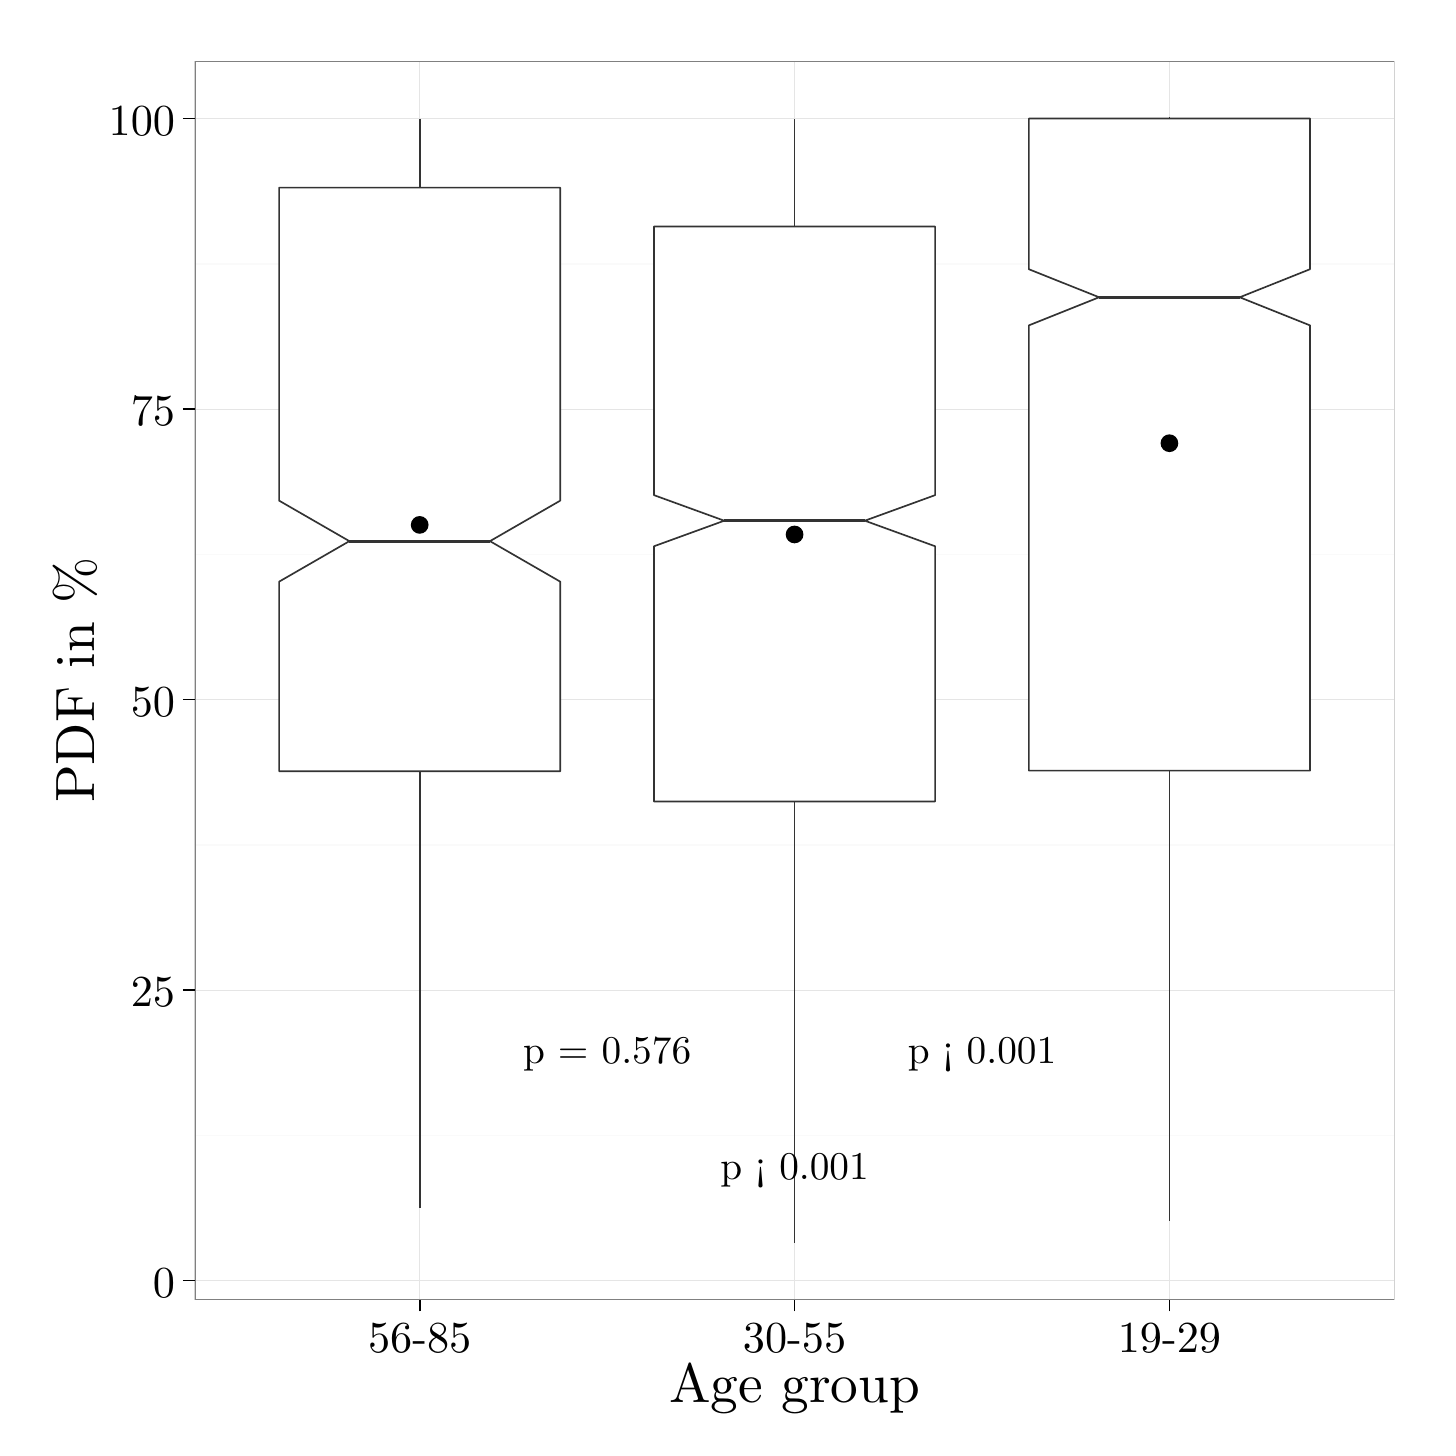
\begin{tikzpicture}[x=1pt,y=1pt]
\definecolor{fillColor}{RGB}{255,255,255}
\path[use as bounding box,fill=fillColor,fill opacity=0.00] (0,0) rectangle (505.89,505.89);
\begin{scope}
\path[clip] (  0.00,  0.00) rectangle (505.89,505.89);
\definecolor{drawColor}{RGB}{255,255,255}
\definecolor{fillColor}{RGB}{255,255,255}

\path[draw=drawColor,line width= 0.6pt,line join=round,line cap=round,fill=fillColor] (  0.00, -0.00) rectangle (505.89,505.89);
\end{scope}
\begin{scope}
\path[clip] ( 60.37, 46.31) rectangle (493.85,493.84);
\definecolor{fillColor}{RGB}{255,255,255}

\path[fill=fillColor] ( 60.37, 46.31) rectangle (493.85,493.84);
\definecolor{drawColor}{gray}{0.98}

\path[draw=drawColor,line width= 0.6pt,line join=round] ( 60.37,105.62) --
	(493.85,105.62);

\path[draw=drawColor,line width= 0.6pt,line join=round] ( 60.37,210.60) --
	(493.85,210.60);

\path[draw=drawColor,line width= 0.6pt,line join=round] ( 60.37,315.57) --
	(493.85,315.57);

\path[draw=drawColor,line width= 0.6pt,line join=round] ( 60.37,420.55) --
	(493.85,420.55);
\definecolor{drawColor}{gray}{0.90}

\path[draw=drawColor,line width= 0.2pt,line join=round] ( 60.37, 53.13) --
	(493.85, 53.13);

\path[draw=drawColor,line width= 0.2pt,line join=round] ( 60.37,158.11) --
	(493.85,158.11);

\path[draw=drawColor,line width= 0.2pt,line join=round] ( 60.37,263.08) --
	(493.85,263.08);

\path[draw=drawColor,line width= 0.2pt,line join=round] ( 60.37,368.06) --
	(493.85,368.06);

\path[draw=drawColor,line width= 0.2pt,line join=round] ( 60.37,473.04) --
	(493.85,473.04);

\path[draw=drawColor,line width= 0.2pt,line join=round] (141.65, 46.31) --
	(141.65,493.84);

\path[draw=drawColor,line width= 0.2pt,line join=round] (277.11, 46.31) --
	(277.11,493.84);

\path[draw=drawColor,line width= 0.2pt,line join=round] (412.57, 46.31) --
	(412.57,493.84);
\definecolor{drawColor}{gray}{0.20}

\path[draw=drawColor,line width= 0.6pt,line join=round] (141.65,448.09) -- (141.65,473.04);

\path[draw=drawColor,line width= 0.6pt,line join=round] (141.65,237.22) -- (141.65, 79.46);

\path[draw=drawColor,line width= 0.6pt,line join=round,line cap=round,fill=fillColor] ( 90.85,448.09) --
	( 90.85,334.98) --
	(116.25,320.34) --
	( 90.85,305.70) --
	( 90.85,237.22) --
	(192.45,237.22) --
	(192.45,305.70) --
	(167.05,320.34) --
	(192.45,334.98) --
	(192.45,448.09) --
	( 90.85,448.09) --
	cycle;

\path[draw=drawColor,line width= 1.1pt,line join=round] (116.25,320.34) -- (167.05,320.34);

\path[draw=drawColor,line width= 0.6pt,line join=round] (277.11,434.04) -- (277.11,473.04);

\path[draw=drawColor,line width= 0.6pt,line join=round] (277.11,226.26) -- (277.11, 66.65);

\path[draw=drawColor,line width= 0.6pt,line join=round,line cap=round,fill=fillColor] (226.31,434.04) --
	(226.31,336.97) --
	(251.71,327.73) --
	(226.31,318.49) --
	(226.31,226.26) --
	(327.91,226.26) --
	(327.91,318.49) --
	(302.51,327.73) --
	(327.91,336.97) --
	(327.91,434.04) --
	(226.31,434.04) --
	cycle;

\path[draw=drawColor,line width= 1.1pt,line join=round] (251.71,327.73) -- (302.51,327.73);

\path[draw=drawColor,line width= 0.6pt,line join=round] (412.57,473.04) -- (412.57,473.50);

\path[draw=drawColor,line width= 0.6pt,line join=round] (412.57,237.41) -- (412.57, 74.80);

\path[draw=drawColor,line width= 0.6pt,line join=round,line cap=round,fill=fillColor] (361.77,473.04) --
	(361.77,418.60) --
	(387.17,408.46) --
	(361.77,398.31) --
	(361.77,237.41) --
	(463.37,237.41) --
	(463.37,398.31) --
	(437.97,408.46) --
	(463.37,418.60) --
	(463.37,473.04) --
	(361.77,473.04) --
	cycle;

\path[draw=drawColor,line width= 1.1pt,line join=round] (387.17,408.46) -- (437.97,408.46);
\definecolor{fillColor}{RGB}{0,0,0}

\path[fill=fillColor] (141.65,326.21) circle (  3.20);

\path[fill=fillColor] (277.11,322.75) circle (  3.20);

\path[fill=fillColor] (412.57,355.73) circle (  3.20);
\definecolor{drawColor}{RGB}{0,0,0}

\node[text=drawColor,anchor=base,inner sep=0pt, outer sep=0pt, scale=  1.42] at (209.38,131.77) {p = 0.576};

\node[text=drawColor,anchor=base,inner sep=0pt, outer sep=0pt, scale=  1.42] at (344.84,131.77) {p < 0.001};

\node[text=drawColor,anchor=base,inner sep=0pt, outer sep=0pt, scale=  1.42] at (277.11, 89.78) {p < 0.001};
\definecolor{drawColor}{gray}{0.50}

\path[draw=drawColor,line width= 0.6pt,line join=round,line cap=round] ( 60.37, 46.31) rectangle (493.85,493.84);
\end{scope}
\begin{scope}
\path[clip] (  0.00,  0.00) rectangle (505.89,505.89);
\definecolor{drawColor}{RGB}{0,0,0}

\node[text=drawColor,anchor=base east,inner sep=0pt, outer sep=0pt, scale=  1.60] at ( 53.26, 47.10) {0};

\node[text=drawColor,anchor=base east,inner sep=0pt, outer sep=0pt, scale=  1.60] at ( 53.26,152.07) {25};

\node[text=drawColor,anchor=base east,inner sep=0pt, outer sep=0pt, scale=  1.60] at ( 53.26,257.05) {50};

\node[text=drawColor,anchor=base east,inner sep=0pt, outer sep=0pt, scale=  1.60] at ( 53.26,362.03) {75};

\node[text=drawColor,anchor=base east,inner sep=0pt, outer sep=0pt, scale=  1.60] at ( 53.26,467.01) {100};
\end{scope}
\begin{scope}
\path[clip] (  0.00,  0.00) rectangle (505.89,505.89);
\definecolor{drawColor}{RGB}{0,0,0}

\path[draw=drawColor,line width= 0.6pt,line join=round] ( 56.10, 53.13) --
	( 60.37, 53.13);

\path[draw=drawColor,line width= 0.6pt,line join=round] ( 56.10,158.11) --
	( 60.37,158.11);

\path[draw=drawColor,line width= 0.6pt,line join=round] ( 56.10,263.08) --
	( 60.37,263.08);

\path[draw=drawColor,line width= 0.6pt,line join=round] ( 56.10,368.06) --
	( 60.37,368.06);

\path[draw=drawColor,line width= 0.6pt,line join=round] ( 56.10,473.04) --
	( 60.37,473.04);
\end{scope}
\begin{scope}
\path[clip] (  0.00,  0.00) rectangle (505.89,505.89);
\definecolor{drawColor}{RGB}{0,0,0}

\path[draw=drawColor,line width= 0.6pt,line join=round] (141.65, 42.04) --
	(141.65, 46.31);

\path[draw=drawColor,line width= 0.6pt,line join=round] (277.11, 42.04) --
	(277.11, 46.31);

\path[draw=drawColor,line width= 0.6pt,line join=round] (412.57, 42.04) --
	(412.57, 46.31);
\end{scope}
\begin{scope}
\path[clip] (  0.00,  0.00) rectangle (505.89,505.89);
\definecolor{drawColor}{RGB}{0,0,0}

\node[text=drawColor,anchor=base,inner sep=0pt, outer sep=0pt, scale=  1.60] at (141.65, 27.13) {56-85};

\node[text=drawColor,anchor=base,inner sep=0pt, outer sep=0pt, scale=  1.60] at (277.11, 27.13) {30-55};

\node[text=drawColor,anchor=base,inner sep=0pt, outer sep=0pt, scale=  1.60] at (412.57, 27.13) {19-29};
\end{scope}
\begin{scope}
\path[clip] (  0.00,  0.00) rectangle (505.89,505.89);
\definecolor{drawColor}{RGB}{0,0,0}

\node[text=drawColor,anchor=base,inner sep=0pt, outer sep=0pt, scale=  2.00] at (277.11,  9.03) {Age group};
\end{scope}
\begin{scope}
\path[clip] (  0.00,  0.00) rectangle (505.89,505.89);
\definecolor{drawColor}{RGB}{0,0,0}

\node[text=drawColor,rotate= 90.00,anchor=base,inner sep=0pt, outer sep=0pt, scale=  2.00] at ( 24.12,270.08) {PDF in {\%}};
\end{scope}
\end{tikzpicture}
} 
	\caption{/k/: PDF by age (released only)}
	\label{fig.box.k.tot}
\end{figure}

Since the age dimension is one of the primary concerns of this study, we will first look at this factor in isolation.
This might seem unnecessary, because the mixed-effects model does not list age group among the significant main effects for predicting \isi{PDF} of /k/.
If we consider a plot of the raw data (\figref{fig.box.k.tot}), however, the picture changes.
First of all, we can see that the upper and lower boundaries of all boxes are around or above 40 and 90\%, respectively.
This means that
\begin{inparaenum}[(a)]
	\item there is a lot of variance in all three groups of speakers, and
	\item all speakers frequently produce /k/ with quite a bit of aspiration, i.e. at least a Scouse ``touch''.
\end{inparaenum}
We also see, however, that the mean (black dots) and median values (thick bars between the notches) remain constant from the old to the middle speakers (t(968.66) = -0.56, p = 0.576), but rise considerably from the middle to the young group (t(2606.825) = 6.886, p < 0.001).
In contrast to the mixed-effects model, t-tests on the raw data thus do find a statistically significant age difference, at least between the middle and the young group.
The cause for these incompatible results is the word \emph{like}.
Due to its role as a fashionable quotative particle, \emph{like} is much more frequent in free speech of the young group (57.89\% of /k/ tokens) than in the middle and old group (39.38 and 26.18\%, respectively).

Young Liverpudlians in this study furthermore realise \emph{like} with a very high average \isi{PDF} of 71.85\% (59.45\% for the middle, 55.59\% for the old group), which contributes considerably to their overall mean visualised in \figref{fig.box.k.tot} and explains part of the interaction of style and age group in the mixed-effects model as well (cf. \figref{fig.line.k.tot}), since it is only in free speech that the preference of young speakers to use \emph{like} (often with a Scouse pronunciation) can fully manifest itself.
If we take out \emph{like} completely, the difference between the oldest and the middle-aged speakers is still not significant (t(900.655) = -0.393, p = 0.694), but that between the middle-aged and the young is (t(1468.008) = 3.999, p < 0.001).
In light of this, I feel justified in claiming that \citeauthor{watson2007a}'s \citeyearpar{watson2007a} finding has been corroborated and that with respect to /k/, Scouse is indeed ``getting Scouser''.

\begin{figure}[h]
	\centering
	\begin{subfigure}{.49\textwidth}
		\centering
			\definecolor{shadecolor}{rgb}{0.969, 0.969, 0.969}
			\resizebox{\linewidth}{!}{% Created by tikzDevice version 0.8.1 on 2016-02-09 02:17:24
% !TEX encoding = UTF-8 Unicode
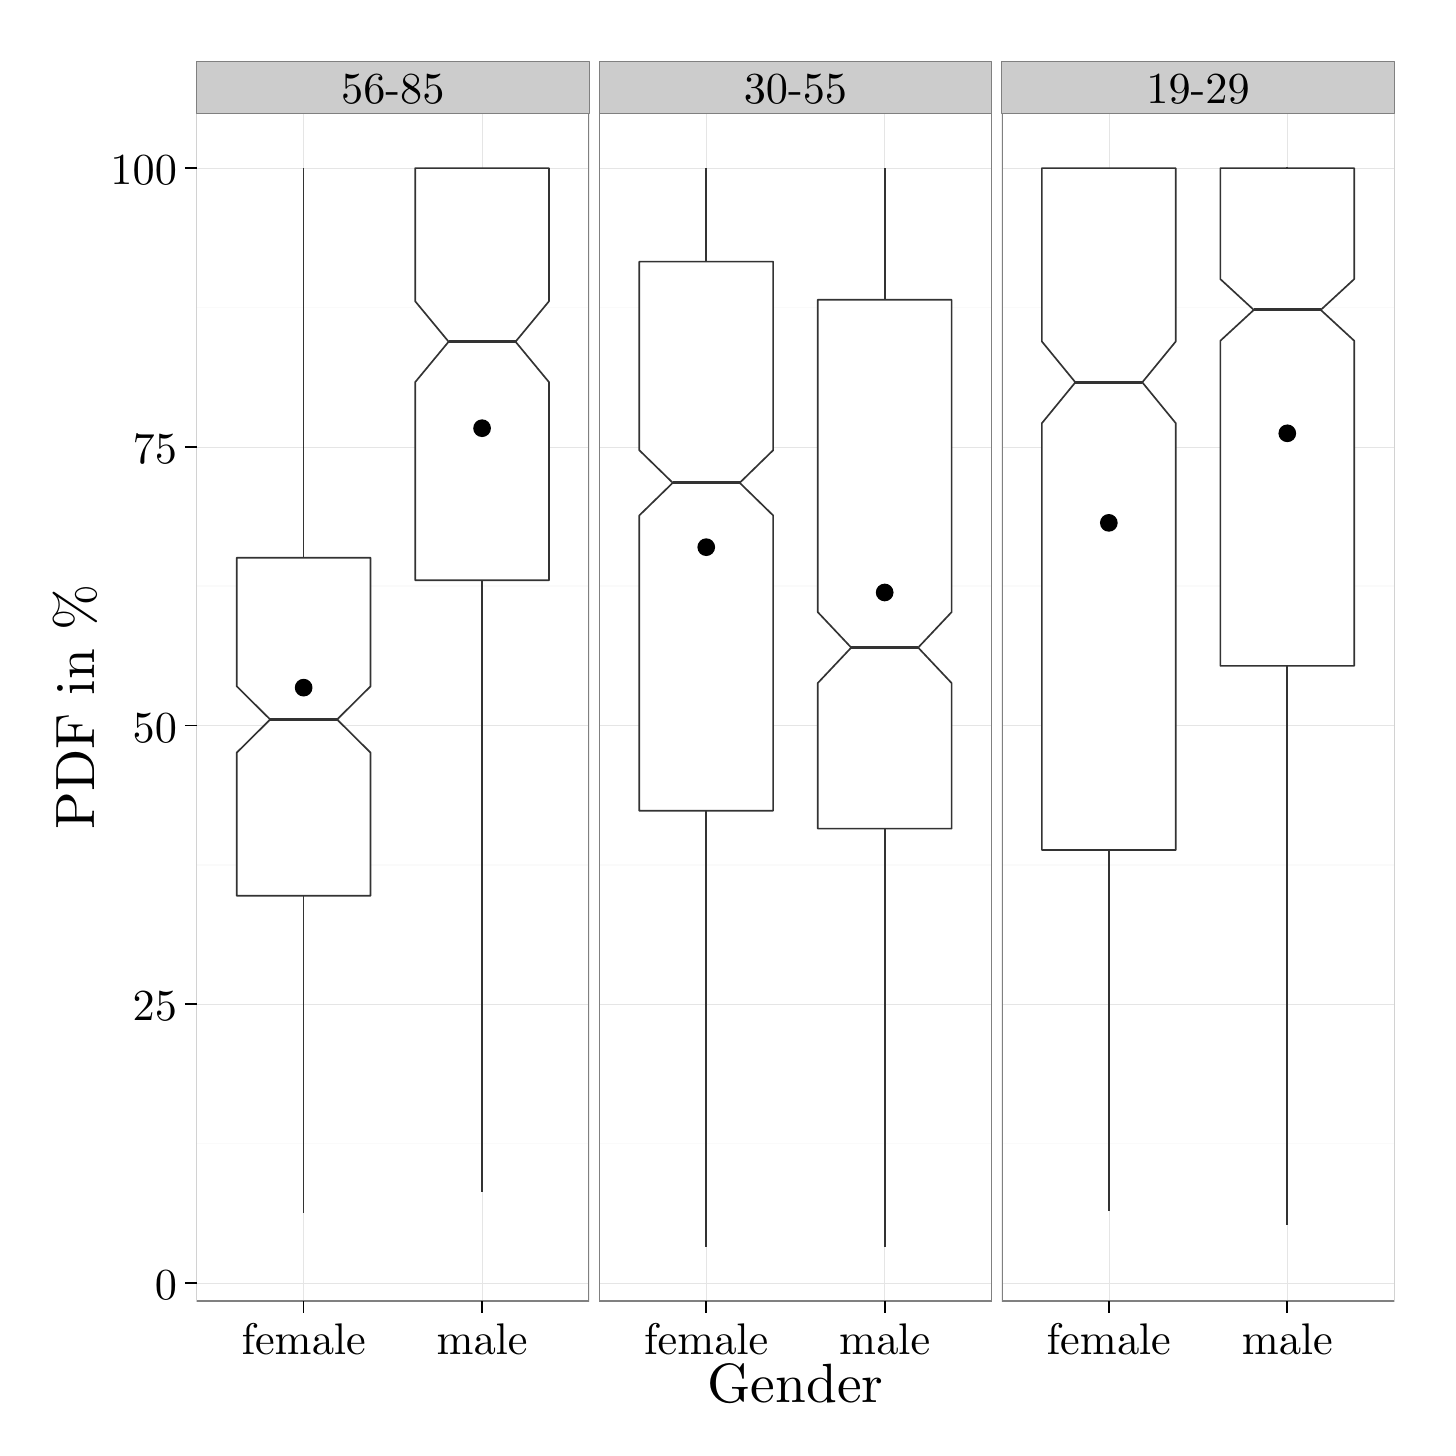
\begin{tikzpicture}[x=1pt,y=1pt]
\definecolor{fillColor}{RGB}{255,255,255}
\path[use as bounding box,fill=fillColor,fill opacity=0.00] (0,0) rectangle (505.89,505.89);
\begin{scope}
\path[clip] (  0.00,  0.00) rectangle (505.89,505.89);
\definecolor{drawColor}{RGB}{255,255,255}
\definecolor{fillColor}{RGB}{255,255,255}

\path[draw=drawColor,line width= 0.6pt,line join=round,line cap=round,fill=fillColor] (  0.00, -0.00) rectangle (505.89,505.89);
\end{scope}
\begin{scope}
\path[clip] ( 61.03, 45.77) rectangle (202.89,475.09);
\definecolor{fillColor}{RGB}{255,255,255}

\path[fill=fillColor] ( 61.03, 45.77) rectangle (202.89,475.09);
\definecolor{drawColor}{gray}{0.98}

\path[draw=drawColor,line width= 0.6pt,line join=round] ( 61.03,102.67) --
	(202.89,102.67);

\path[draw=drawColor,line width= 0.6pt,line join=round] ( 61.03,203.37) --
	(202.89,203.37);

\path[draw=drawColor,line width= 0.6pt,line join=round] ( 61.03,304.07) --
	(202.89,304.07);

\path[draw=drawColor,line width= 0.6pt,line join=round] ( 61.03,404.78) --
	(202.89,404.78);
\definecolor{drawColor}{gray}{0.90}

\path[draw=drawColor,line width= 0.2pt,line join=round] ( 61.03, 52.32) --
	(202.89, 52.32);

\path[draw=drawColor,line width= 0.2pt,line join=round] ( 61.03,153.02) --
	(202.89,153.02);

\path[draw=drawColor,line width= 0.2pt,line join=round] ( 61.03,253.72) --
	(202.89,253.72);

\path[draw=drawColor,line width= 0.2pt,line join=round] ( 61.03,354.43) --
	(202.89,354.43);

\path[draw=drawColor,line width= 0.2pt,line join=round] ( 61.03,455.13) --
	(202.89,455.13);

\path[draw=drawColor,line width= 0.2pt,line join=round] ( 99.72, 45.77) --
	( 99.72,475.09);

\path[draw=drawColor,line width= 0.2pt,line join=round] (164.20, 45.77) --
	(164.20,475.09);
\definecolor{drawColor}{gray}{0.20}

\path[draw=drawColor,line width= 0.6pt,line join=round] ( 99.72,314.37) -- ( 99.72,455.13);

\path[draw=drawColor,line width= 0.6pt,line join=round] ( 99.72,192.23) -- ( 99.72, 77.57);

\path[draw=drawColor,line width= 0.6pt,line join=round,line cap=round,fill=fillColor] ( 75.54,314.37) --
	( 75.54,267.89) --
	( 87.63,255.90) --
	( 75.54,243.91) --
	( 75.54,192.23) --
	(123.90,192.23) --
	(123.90,243.91) --
	(111.81,255.90) --
	(123.90,267.89) --
	(123.90,314.37) --
	( 75.54,314.37) --
	cycle;

\path[draw=drawColor,line width= 1.1pt,line join=round] ( 87.63,255.90) -- (111.81,255.90);

\path[draw=drawColor,line width= 0.6pt,line join=round] (164.20,455.13) -- (164.20,455.13);

\path[draw=drawColor,line width= 0.6pt,line join=round] (164.20,306.21) -- (164.20, 85.15);

\path[draw=drawColor,line width= 0.6pt,line join=round,line cap=round,fill=fillColor] (140.02,455.13) --
	(140.02,407.03) --
	(152.11,392.41) --
	(140.02,377.79) --
	(140.02,306.21) --
	(188.38,306.21) --
	(188.38,377.79) --
	(176.29,392.41) --
	(188.38,407.03) --
	(188.38,455.13) --
	(140.02,455.13) --
	cycle;

\path[draw=drawColor,line width= 1.1pt,line join=round] (152.11,392.41) -- (176.29,392.41);
\definecolor{fillColor}{RGB}{0,0,0}

\path[fill=fillColor] ( 99.72,267.40) circle (  3.20);

\path[fill=fillColor] (164.20,361.15) circle (  3.20);
\definecolor{drawColor}{gray}{0.50}

\path[draw=drawColor,line width= 0.6pt,line join=round,line cap=round] ( 61.03, 45.77) rectangle (202.89,475.09);
\end{scope}
\begin{scope}
\path[clip] (206.51, 45.77) rectangle (348.37,475.09);
\definecolor{fillColor}{RGB}{255,255,255}

\path[fill=fillColor] (206.51, 45.77) rectangle (348.37,475.09);
\definecolor{drawColor}{gray}{0.98}

\path[draw=drawColor,line width= 0.6pt,line join=round] (206.51,102.67) --
	(348.37,102.67);

\path[draw=drawColor,line width= 0.6pt,line join=round] (206.51,203.37) --
	(348.37,203.37);

\path[draw=drawColor,line width= 0.6pt,line join=round] (206.51,304.07) --
	(348.37,304.07);

\path[draw=drawColor,line width= 0.6pt,line join=round] (206.51,404.78) --
	(348.37,404.78);
\definecolor{drawColor}{gray}{0.90}

\path[draw=drawColor,line width= 0.2pt,line join=round] (206.51, 52.32) --
	(348.37, 52.32);

\path[draw=drawColor,line width= 0.2pt,line join=round] (206.51,153.02) --
	(348.37,153.02);

\path[draw=drawColor,line width= 0.2pt,line join=round] (206.51,253.72) --
	(348.37,253.72);

\path[draw=drawColor,line width= 0.2pt,line join=round] (206.51,354.43) --
	(348.37,354.43);

\path[draw=drawColor,line width= 0.2pt,line join=round] (206.51,455.13) --
	(348.37,455.13);

\path[draw=drawColor,line width= 0.2pt,line join=round] (245.20, 45.77) --
	(245.20,475.09);

\path[draw=drawColor,line width= 0.2pt,line join=round] (309.68, 45.77) --
	(309.68,475.09);
\definecolor{drawColor}{gray}{0.20}

\path[draw=drawColor,line width= 0.6pt,line join=round] (245.20,421.33) -- (245.20,455.13);

\path[draw=drawColor,line width= 0.6pt,line join=round] (245.20,222.93) -- (245.20, 65.29);

\path[draw=drawColor,line width= 0.6pt,line join=round,line cap=round,fill=fillColor] (221.01,421.33) --
	(221.01,353.20) --
	(233.10,341.42) --
	(221.01,329.63) --
	(221.01,222.93) --
	(269.38,222.93) --
	(269.38,329.63) --
	(257.29,341.42) --
	(269.38,353.20) --
	(269.38,421.33) --
	(221.01,421.33) --
	cycle;

\path[draw=drawColor,line width= 1.1pt,line join=round] (233.10,341.42) -- (257.29,341.42);

\path[draw=drawColor,line width= 0.6pt,line join=round] (309.68,407.56) -- (309.68,455.13);

\path[draw=drawColor,line width= 0.6pt,line join=round] (309.68,216.46) -- (309.68, 65.45);

\path[draw=drawColor,line width= 0.6pt,line join=round,line cap=round,fill=fillColor] (285.50,407.56) --
	(285.50,294.70) --
	(297.59,281.88) --
	(285.50,269.06) --
	(285.50,216.46) --
	(333.86,216.46) --
	(333.86,269.06) --
	(321.77,281.88) --
	(333.86,294.70) --
	(333.86,407.56) --
	(285.50,407.56) --
	cycle;

\path[draw=drawColor,line width= 1.1pt,line join=round] (297.59,281.88) -- (321.77,281.88);
\definecolor{fillColor}{RGB}{0,0,0}

\path[fill=fillColor] (245.20,318.16) circle (  3.20);

\path[fill=fillColor] (309.68,301.79) circle (  3.20);
\definecolor{drawColor}{gray}{0.50}

\path[draw=drawColor,line width= 0.6pt,line join=round,line cap=round] (206.51, 45.77) rectangle (348.37,475.09);
\end{scope}
\begin{scope}
\path[clip] (351.98, 45.77) rectangle (493.85,475.09);
\definecolor{fillColor}{RGB}{255,255,255}

\path[fill=fillColor] (351.98, 45.77) rectangle (493.85,475.09);
\definecolor{drawColor}{gray}{0.98}

\path[draw=drawColor,line width= 0.6pt,line join=round] (351.98,102.67) --
	(493.85,102.67);

\path[draw=drawColor,line width= 0.6pt,line join=round] (351.98,203.37) --
	(493.85,203.37);

\path[draw=drawColor,line width= 0.6pt,line join=round] (351.98,304.07) --
	(493.85,304.07);

\path[draw=drawColor,line width= 0.6pt,line join=round] (351.98,404.78) --
	(493.85,404.78);
\definecolor{drawColor}{gray}{0.90}

\path[draw=drawColor,line width= 0.2pt,line join=round] (351.98, 52.32) --
	(493.85, 52.32);

\path[draw=drawColor,line width= 0.2pt,line join=round] (351.98,153.02) --
	(493.85,153.02);

\path[draw=drawColor,line width= 0.2pt,line join=round] (351.98,253.72) --
	(493.85,253.72);

\path[draw=drawColor,line width= 0.2pt,line join=round] (351.98,354.43) --
	(493.85,354.43);

\path[draw=drawColor,line width= 0.2pt,line join=round] (351.98,455.13) --
	(493.85,455.13);

\path[draw=drawColor,line width= 0.2pt,line join=round] (390.67, 45.77) --
	(390.67,475.09);

\path[draw=drawColor,line width= 0.2pt,line join=round] (455.16, 45.77) --
	(455.16,475.09);
\definecolor{drawColor}{gray}{0.20}

\path[draw=drawColor,line width= 0.6pt,line join=round] (390.67,455.13) -- (390.67,455.13);

\path[draw=drawColor,line width= 0.6pt,line join=round] (390.67,208.76) -- (390.67, 78.18);

\path[draw=drawColor,line width= 0.6pt,line join=round,line cap=round,fill=fillColor] (366.49,455.13) --
	(366.49,392.48) --
	(378.58,377.73) --
	(366.49,362.97) --
	(366.49,208.76) --
	(414.85,208.76) --
	(414.85,362.97) --
	(402.76,377.73) --
	(414.85,392.48) --
	(414.85,455.13) --
	(366.49,455.13) --
	cycle;

\path[draw=drawColor,line width= 1.1pt,line join=round] (378.58,377.73) -- (402.76,377.73);

\path[draw=drawColor,line width= 0.6pt,line join=round] (455.16,455.13) -- (455.16,455.57);

\path[draw=drawColor,line width= 0.6pt,line join=round] (455.16,275.27) -- (455.16, 73.10);

\path[draw=drawColor,line width= 0.6pt,line join=round,line cap=round,fill=fillColor] (430.97,455.13) --
	(430.97,415.03) --
	(443.06,403.89) --
	(430.97,392.75) --
	(430.97,275.27) --
	(479.34,275.27) --
	(479.34,392.75) --
	(467.25,403.89) --
	(479.34,415.03) --
	(479.34,455.13) --
	(430.97,455.13) --
	cycle;

\path[draw=drawColor,line width= 1.1pt,line join=round] (443.06,403.89) -- (467.25,403.89);
\definecolor{fillColor}{RGB}{0,0,0}

\path[fill=fillColor] (390.67,326.95) circle (  3.20);

\path[fill=fillColor] (455.16,359.31) circle (  3.20);
\definecolor{drawColor}{gray}{0.50}

\path[draw=drawColor,line width= 0.6pt,line join=round,line cap=round] (351.98, 45.77) rectangle (493.85,475.09);
\end{scope}
\begin{scope}
\path[clip] (  0.00,  0.00) rectangle (505.89,505.89);
\definecolor{drawColor}{gray}{0.50}
\definecolor{fillColor}{gray}{0.80}

\path[draw=drawColor,line width= 0.2pt,line join=round,line cap=round,fill=fillColor] ( 61.03,475.09) rectangle (202.89,493.85);
\definecolor{drawColor}{RGB}{0,0,0}

\node[text=drawColor,anchor=base,inner sep=0pt, outer sep=0pt, scale=  1.60] at (131.96,478.43) {56-85};
\end{scope}
\begin{scope}
\path[clip] (  0.00,  0.00) rectangle (505.89,505.89);
\definecolor{drawColor}{gray}{0.50}
\definecolor{fillColor}{gray}{0.80}

\path[draw=drawColor,line width= 0.2pt,line join=round,line cap=round,fill=fillColor] (206.51,475.09) rectangle (348.37,493.85);
\definecolor{drawColor}{RGB}{0,0,0}

\node[text=drawColor,anchor=base,inner sep=0pt, outer sep=0pt, scale=  1.60] at (277.44,478.43) {30-55};
\end{scope}
\begin{scope}
\path[clip] (  0.00,  0.00) rectangle (505.89,505.89);
\definecolor{drawColor}{gray}{0.50}
\definecolor{fillColor}{gray}{0.80}

\path[draw=drawColor,line width= 0.2pt,line join=round,line cap=round,fill=fillColor] (351.98,475.09) rectangle (493.85,493.85);
\definecolor{drawColor}{RGB}{0,0,0}

\node[text=drawColor,anchor=base,inner sep=0pt, outer sep=0pt, scale=  1.60] at (422.91,478.43) {19-29};
\end{scope}
\begin{scope}
\path[clip] (  0.00,  0.00) rectangle (505.89,505.89);
\definecolor{drawColor}{RGB}{0,0,0}

\node[text=drawColor,anchor=base east,inner sep=0pt, outer sep=0pt, scale=  1.60] at ( 53.92, 46.28) {0};

\node[text=drawColor,anchor=base east,inner sep=0pt, outer sep=0pt, scale=  1.60] at ( 53.92,146.99) {25};

\node[text=drawColor,anchor=base east,inner sep=0pt, outer sep=0pt, scale=  1.60] at ( 53.92,247.69) {50};

\node[text=drawColor,anchor=base east,inner sep=0pt, outer sep=0pt, scale=  1.60] at ( 53.92,348.39) {75};

\node[text=drawColor,anchor=base east,inner sep=0pt, outer sep=0pt, scale=  1.60] at ( 53.92,449.10) {100};
\end{scope}
\begin{scope}
\path[clip] (  0.00,  0.00) rectangle (505.89,505.89);
\definecolor{drawColor}{RGB}{0,0,0}

\path[draw=drawColor,line width= 0.6pt,line join=round] ( 56.76, 52.32) --
	( 61.03, 52.32);

\path[draw=drawColor,line width= 0.6pt,line join=round] ( 56.76,153.02) --
	( 61.03,153.02);

\path[draw=drawColor,line width= 0.6pt,line join=round] ( 56.76,253.72) --
	( 61.03,253.72);

\path[draw=drawColor,line width= 0.6pt,line join=round] ( 56.76,354.43) --
	( 61.03,354.43);

\path[draw=drawColor,line width= 0.6pt,line join=round] ( 56.76,455.13) --
	( 61.03,455.13);
\end{scope}
\begin{scope}
\path[clip] (  0.00,  0.00) rectangle (505.89,505.89);
\definecolor{drawColor}{RGB}{0,0,0}

\path[draw=drawColor,line width= 0.6pt,line join=round] ( 99.72, 41.50) --
	( 99.72, 45.77);

\path[draw=drawColor,line width= 0.6pt,line join=round] (164.20, 41.50) --
	(164.20, 45.77);
\end{scope}
\begin{scope}
\path[clip] (  0.00,  0.00) rectangle (505.89,505.89);
\definecolor{drawColor}{RGB}{0,0,0}

\node[text=drawColor,anchor=base,inner sep=0pt, outer sep=0pt, scale=  1.60] at ( 99.72, 26.59) {female};

\node[text=drawColor,anchor=base,inner sep=0pt, outer sep=0pt, scale=  1.60] at (164.20, 26.59) {male};
\end{scope}
\begin{scope}
\path[clip] (  0.00,  0.00) rectangle (505.89,505.89);
\definecolor{drawColor}{RGB}{0,0,0}

\path[draw=drawColor,line width= 0.6pt,line join=round] (245.20, 41.50) --
	(245.20, 45.77);

\path[draw=drawColor,line width= 0.6pt,line join=round] (309.68, 41.50) --
	(309.68, 45.77);
\end{scope}
\begin{scope}
\path[clip] (  0.00,  0.00) rectangle (505.89,505.89);
\definecolor{drawColor}{RGB}{0,0,0}

\node[text=drawColor,anchor=base,inner sep=0pt, outer sep=0pt, scale=  1.60] at (245.20, 26.59) {female};

\node[text=drawColor,anchor=base,inner sep=0pt, outer sep=0pt, scale=  1.60] at (309.68, 26.59) {male};
\end{scope}
\begin{scope}
\path[clip] (  0.00,  0.00) rectangle (505.89,505.89);
\definecolor{drawColor}{RGB}{0,0,0}

\path[draw=drawColor,line width= 0.6pt,line join=round] (390.67, 41.50) --
	(390.67, 45.77);

\path[draw=drawColor,line width= 0.6pt,line join=round] (455.16, 41.50) --
	(455.16, 45.77);
\end{scope}
\begin{scope}
\path[clip] (  0.00,  0.00) rectangle (505.89,505.89);
\definecolor{drawColor}{RGB}{0,0,0}

\node[text=drawColor,anchor=base,inner sep=0pt, outer sep=0pt, scale=  1.60] at (390.67, 26.59) {female};

\node[text=drawColor,anchor=base,inner sep=0pt, outer sep=0pt, scale=  1.60] at (455.16, 26.59) {male};
\end{scope}
\begin{scope}
\path[clip] (  0.00,  0.00) rectangle (505.89,505.89);
\definecolor{drawColor}{RGB}{0,0,0}

\node[text=drawColor,anchor=base,inner sep=0pt, outer sep=0pt, scale=  2.00] at (277.44,  9.03) {Gender};
\end{scope}
\begin{scope}
\path[clip] (  0.00,  0.00) rectangle (505.89,505.89);
\definecolor{drawColor}{RGB}{0,0,0}

\node[text=drawColor,rotate= 90.00,anchor=base,inner sep=0pt, outer sep=0pt, scale=  2.00] at ( 24.12,260.43) {PDF in {\%}};
\end{scope}
\end{tikzpicture}
} 
		\caption{box plot}
		\label{fig.box.k.agegender}
	\end{subfigure}
	\begin{subfigure}{.49\textwidth}
		\centering
			\definecolor{shadecolor}{rgb}{0.969, 0.969, 0.969}
			\resizebox{\linewidth}{!}{% Created by tikzDevice version 0.8.1 on 2016-02-09 02:17:24
% !TEX encoding = UTF-8 Unicode
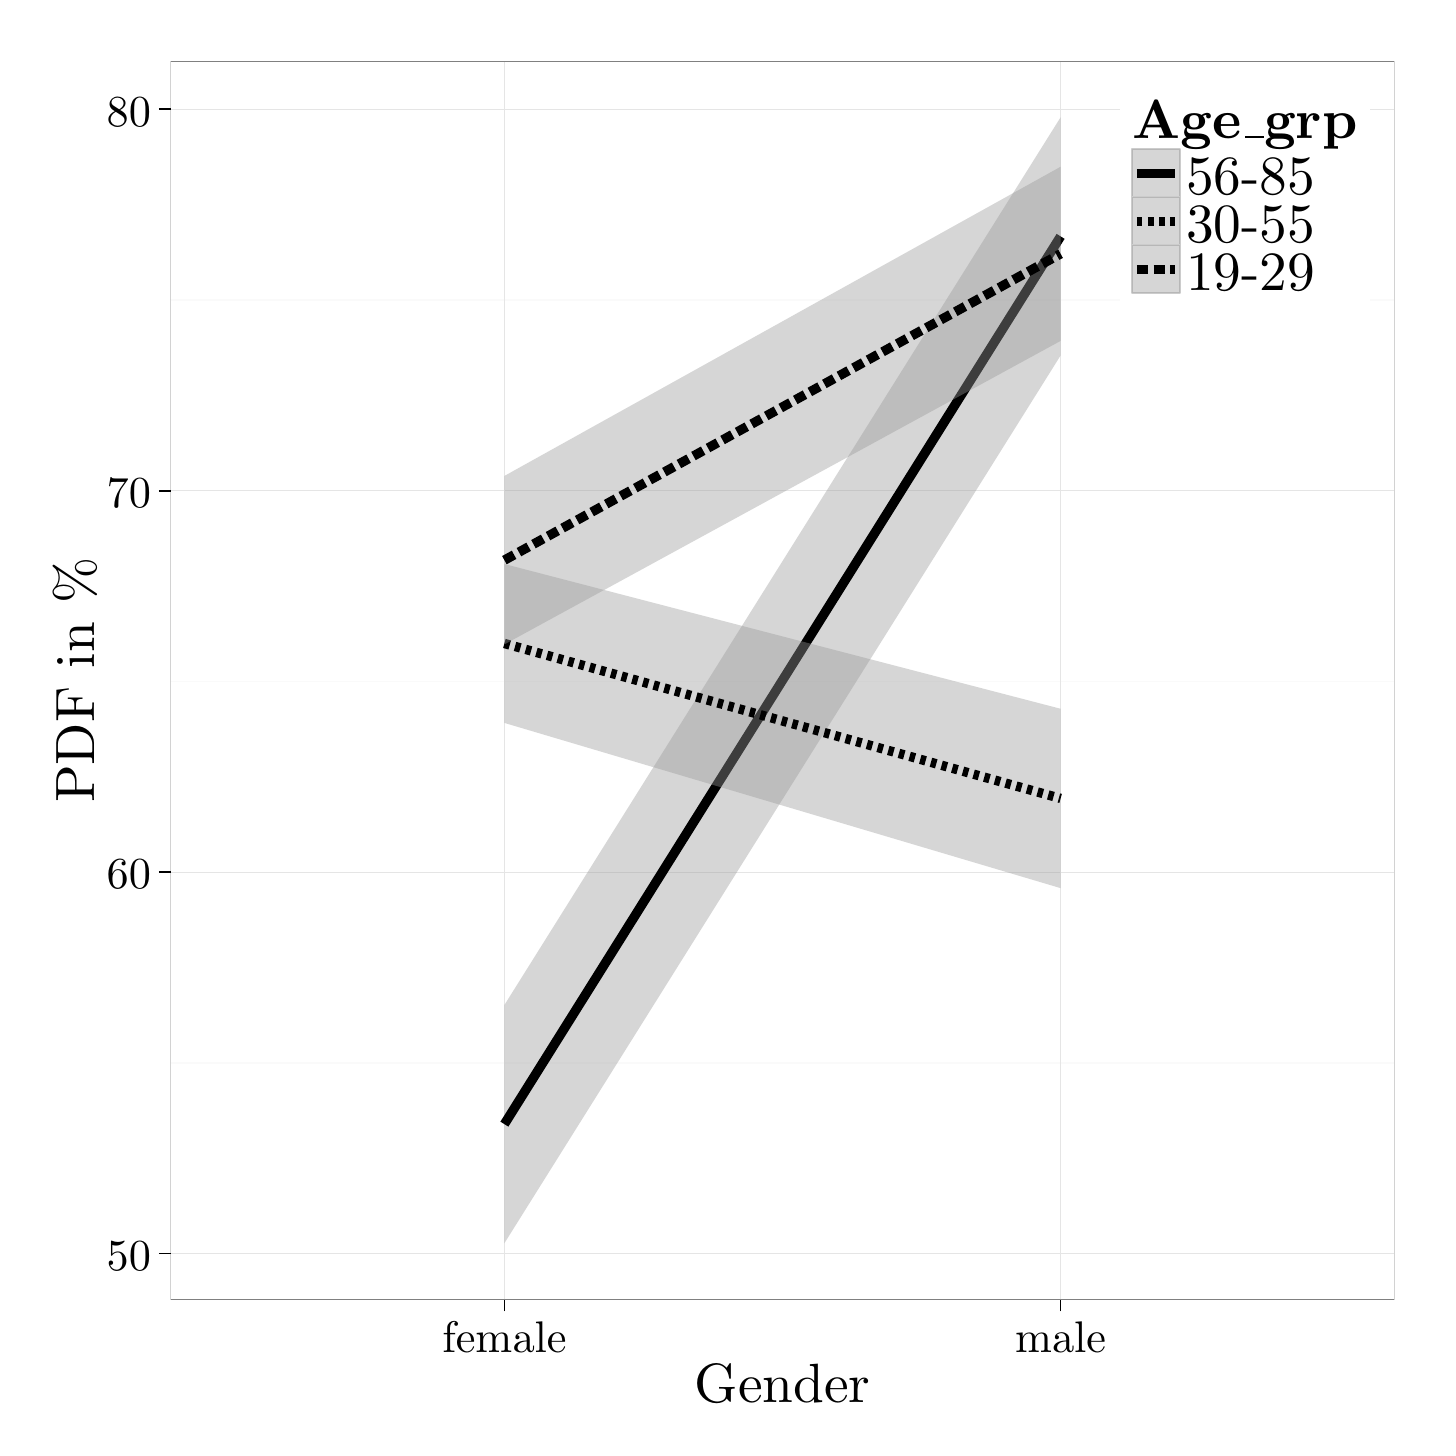
\begin{tikzpicture}[x=1pt,y=1pt]
\definecolor{fillColor}{RGB}{255,255,255}
\path[use as bounding box,fill=fillColor,fill opacity=0.00] (0,0) rectangle (505.89,505.89);
\begin{scope}
\path[clip] (  0.00,  0.00) rectangle (505.89,505.89);
\definecolor{drawColor}{RGB}{255,255,255}
\definecolor{fillColor}{RGB}{255,255,255}

\path[draw=drawColor,line width= 0.6pt,line join=round,line cap=round,fill=fillColor] (  0.00, -0.00) rectangle (505.89,505.89);
\end{scope}
\begin{scope}
\path[clip] ( 51.66, 46.31) rectangle (493.85,493.84);
\definecolor{fillColor}{RGB}{255,255,255}

\path[fill=fillColor] ( 51.66, 46.31) rectangle (493.84,493.84);
\definecolor{drawColor}{gray}{0.98}

\path[draw=drawColor,line width= 0.6pt,line join=round] ( 51.66,131.81) --
	(493.85,131.81);

\path[draw=drawColor,line width= 0.6pt,line join=round] ( 51.66,269.63) --
	(493.85,269.63);

\path[draw=drawColor,line width= 0.6pt,line join=round] ( 51.66,407.46) --
	(493.85,407.46);
\definecolor{drawColor}{gray}{0.90}

\path[draw=drawColor,line width= 0.2pt,line join=round] ( 51.66, 62.89) --
	(493.85, 62.89);

\path[draw=drawColor,line width= 0.2pt,line join=round] ( 51.66,200.72) --
	(493.85,200.72);

\path[draw=drawColor,line width= 0.2pt,line join=round] ( 51.66,338.55) --
	(493.85,338.55);

\path[draw=drawColor,line width= 0.2pt,line join=round] ( 51.66,476.38) --
	(493.85,476.38);

\path[draw=drawColor,line width= 0.2pt,line join=round] (172.26, 46.31) --
	(172.26,493.84);

\path[draw=drawColor,line width= 0.2pt,line join=round] (373.25, 46.31) --
	(373.25,493.84);
\definecolor{fillColor}{RGB}{153,153,153}

\path[fill=fillColor,fill opacity=0.40] (172.26,152.72) --
	(373.25,473.50) --
	(373.25,387.44) --
	(172.26, 66.65) --
	cycle;
\definecolor{drawColor}{RGB}{0,0,0}

\path[draw=drawColor,line width= 3.4pt,line join=round] (172.26,109.68) --
	(373.25,430.47);

\path[fill=fillColor,fill opacity=0.40] (172.26,312.08) --
	(373.25,259.77) --
	(373.25,194.96) --
	(172.26,254.66) --
	cycle;

\path[draw=drawColor,line width= 3.4pt,dash pattern=on 2pt off 2pt ,line join=round] (172.26,283.37) --
	(373.25,227.37);

\path[fill=fillColor,fill opacity=0.40] (172.26,343.90) --
	(373.25,455.64) --
	(373.25,392.70) --
	(172.26,283.03) --
	cycle;

\path[draw=drawColor,line width= 3.4pt,dash pattern=on 4pt off 2pt ,line join=round] (172.26,313.47) --
	(373.25,424.17);
\definecolor{drawColor}{gray}{0.50}

\path[draw=drawColor,line width= 0.6pt,line join=round,line cap=round] ( 51.66, 46.31) rectangle (493.84,493.84);
\end{scope}
\begin{scope}
\path[clip] (  0.00,  0.00) rectangle (505.89,505.89);
\definecolor{drawColor}{RGB}{0,0,0}

\node[text=drawColor,anchor=base east,inner sep=0pt, outer sep=0pt, scale=  1.60] at ( 44.55, 56.86) {50};

\node[text=drawColor,anchor=base east,inner sep=0pt, outer sep=0pt, scale=  1.60] at ( 44.55,194.69) {60};

\node[text=drawColor,anchor=base east,inner sep=0pt, outer sep=0pt, scale=  1.60] at ( 44.55,332.52) {70};

\node[text=drawColor,anchor=base east,inner sep=0pt, outer sep=0pt, scale=  1.60] at ( 44.55,470.34) {80};
\end{scope}
\begin{scope}
\path[clip] (  0.00,  0.00) rectangle (505.89,505.89);
\definecolor{drawColor}{RGB}{0,0,0}

\path[draw=drawColor,line width= 0.6pt,line join=round] ( 47.39, 62.89) --
	( 51.66, 62.89);

\path[draw=drawColor,line width= 0.6pt,line join=round] ( 47.39,200.72) --
	( 51.66,200.72);

\path[draw=drawColor,line width= 0.6pt,line join=round] ( 47.39,338.55) --
	( 51.66,338.55);

\path[draw=drawColor,line width= 0.6pt,line join=round] ( 47.39,476.38) --
	( 51.66,476.38);
\end{scope}
\begin{scope}
\path[clip] (  0.00,  0.00) rectangle (505.89,505.89);
\definecolor{drawColor}{RGB}{0,0,0}

\path[draw=drawColor,line width= 0.6pt,line join=round] (172.26, 42.04) --
	(172.26, 46.31);

\path[draw=drawColor,line width= 0.6pt,line join=round] (373.25, 42.04) --
	(373.25, 46.31);
\end{scope}
\begin{scope}
\path[clip] (  0.00,  0.00) rectangle (505.89,505.89);
\definecolor{drawColor}{RGB}{0,0,0}

\node[text=drawColor,anchor=base,inner sep=0pt, outer sep=0pt, scale=  1.60] at (172.26, 27.13) {female};

\node[text=drawColor,anchor=base,inner sep=0pt, outer sep=0pt, scale=  1.60] at (373.25, 27.13) {male};
\end{scope}
\begin{scope}
\path[clip] (  0.00,  0.00) rectangle (505.89,505.89);
\definecolor{drawColor}{RGB}{0,0,0}

\node[text=drawColor,anchor=base,inner sep=0pt, outer sep=0pt, scale=  2.00] at (272.75,  9.03) {Gender};
\end{scope}
\begin{scope}
\path[clip] (  0.00,  0.00) rectangle (505.89,505.89);
\definecolor{drawColor}{RGB}{0,0,0}

\node[text=drawColor,rotate= 90.00,anchor=base,inner sep=0pt, outer sep=0pt, scale=  2.00] at ( 24.12,270.08) {PDF in {\%}};
\end{scope}
\begin{scope}
\path[clip] (  0.00,  0.00) rectangle (505.89,505.89);
\definecolor{fillColor}{RGB}{255,255,255}

\path[fill=fillColor] (394.82,405.66) rectangle (484.98,484.98);
\end{scope}
\begin{scope}
\path[clip] (  0.00,  0.00) rectangle (505.89,505.89);
\definecolor{drawColor}{RGB}{0,0,0}

\node[text=drawColor,anchor=base west,inner sep=0pt, outer sep=0pt, scale=  2.00] at (399.08,465.96) {\bfseries Age{\_{}}grp};
\end{scope}
\begin{scope}
\path[clip] (  0.00,  0.00) rectangle (505.89,505.89);
\definecolor{drawColor}{gray}{0.80}
\definecolor{fillColor}{RGB}{255,255,255}

\path[draw=drawColor,line width= 0.6pt,line join=round,line cap=round,fill=fillColor] (399.08,444.61) rectangle (416.43,461.96);
\end{scope}
\begin{scope}
\path[clip] (  0.00,  0.00) rectangle (505.89,505.89);
\definecolor{fillColor}{RGB}{153,153,153}

\path[fill=fillColor,fill opacity=0.40] (399.08,444.61) rectangle (416.43,461.96);
\definecolor{drawColor}{RGB}{0,0,0}

\path[draw=drawColor,line width= 3.4pt,line join=round] (400.82,453.29) -- (414.69,453.29);
\end{scope}
\begin{scope}
\path[clip] (  0.00,  0.00) rectangle (505.89,505.89);
\definecolor{drawColor}{gray}{0.80}
\definecolor{fillColor}{RGB}{255,255,255}

\path[draw=drawColor,line width= 0.6pt,line join=round,line cap=round,fill=fillColor] (399.08,427.27) rectangle (416.43,444.61);
\end{scope}
\begin{scope}
\path[clip] (  0.00,  0.00) rectangle (505.89,505.89);
\definecolor{fillColor}{RGB}{153,153,153}

\path[fill=fillColor,fill opacity=0.40] (399.08,427.27) rectangle (416.43,444.61);
\definecolor{drawColor}{RGB}{0,0,0}

\path[draw=drawColor,line width= 3.4pt,dash pattern=on 2pt off 2pt ,line join=round] (400.82,435.94) -- (414.69,435.94);
\end{scope}
\begin{scope}
\path[clip] (  0.00,  0.00) rectangle (505.89,505.89);
\definecolor{drawColor}{gray}{0.80}
\definecolor{fillColor}{RGB}{255,255,255}

\path[draw=drawColor,line width= 0.6pt,line join=round,line cap=round,fill=fillColor] (399.08,409.92) rectangle (416.43,427.27);
\end{scope}
\begin{scope}
\path[clip] (  0.00,  0.00) rectangle (505.89,505.89);
\definecolor{fillColor}{RGB}{153,153,153}

\path[fill=fillColor,fill opacity=0.40] (399.08,409.92) rectangle (416.43,427.27);
\definecolor{drawColor}{RGB}{0,0,0}

\path[draw=drawColor,line width= 3.4pt,dash pattern=on 4pt off 2pt ,line join=round] (400.82,418.60) -- (414.69,418.60);
\end{scope}
\begin{scope}
\path[clip] (  0.00,  0.00) rectangle (505.89,505.89);
\definecolor{drawColor}{RGB}{0,0,0}

\node[text=drawColor,anchor=base west,inner sep=0pt, outer sep=0pt, scale=  2.00] at (418.60,445.75) {56-85};
\end{scope}
\begin{scope}
\path[clip] (  0.00,  0.00) rectangle (505.89,505.89);
\definecolor{drawColor}{RGB}{0,0,0}

\node[text=drawColor,anchor=base west,inner sep=0pt, outer sep=0pt, scale=  2.00] at (418.60,428.40) {30-55};
\end{scope}
\begin{scope}
\path[clip] (  0.00,  0.00) rectangle (505.89,505.89);
\definecolor{drawColor}{RGB}{0,0,0}

\node[text=drawColor,anchor=base west,inner sep=0pt, outer sep=0pt, scale=  2.00] at (418.60,411.06) {19-29};
\end{scope}
\end{tikzpicture}
}
		\caption{regression plot}
		\label{fig.scatter.k.agegender}
	\end{subfigure}
	\caption{/k/: PDF by age and gender (released only)}
\end{figure}

At least this is true if we pool the data for all subjects and only focus on the age dimension.
However, the mixed linear effects regression found significant interactions of age with gender and social class as well, so a more detailed account of the impact of the predictor age is necessary.
In \figref{fig.box.k.agegender} the gender difference in the individual age groups is visualised in three separate box plots.
The oldest speakers (left panel) show a very pronounced gender difference in the expected direction: women have both a lower mean and median than men, i.e. the former use less lenition than the latter.
Both groups also show comparatively little variation around the mean, and in consequence there is only a very small overlap of the interquartile ranges (vertical extent of the boxes).
It is therefore not surprising that a t-test finds the gender difference to be highly significant in this age group (t(515.826) = -10.356, p < 0.001).
For middle-aged speakers (panel in the middle), things seem to be a lot less clear.
Women and men have clearly distinct\is{distinctness} medians in this age group (no overlapping notches), but it is now the men who have lower \isi{PDF} values than the women.
The same goes for the mean, which is also lower for men than for women.
However, it should be noted that the two genders are somewhat less distinct\is{distinctness} in this sub-sample due to increased variation in both groups (the interquartile ranges occupy virtually the same space).
Nevertheless this difference is still statistically significant (t(1198.637) = 2.543, p = 0.011).
When we focus on the youngest speakers in the sample, we find that
\begin{inparaenum}[(a)]
	\item the gender distinction has become (even) more statistically robust again (t(1339.877) = -4.982, p < 0.001), and
	\item it is now once more the female speakers who are less Scouse than their male counterparts (cf. the old group).
\end{inparaenum}

\begin{table}[h]
	\centering
	\caption{/k/: t-tests of age by gender}
	\label{tab.k.genderage.pvalues}
	\begin{tabular}{lrrrrrr}
		\toprule
		test & \multicolumn{3}{c}{women} & \multicolumn{3}{c}{men}\\
		& t & df & p & t & df & p\\
		\midrule
		old-middle & 6.537 & 502.217 & < 0.001 & \ensuremath{-7.473} & 551.684 & < 0.001\\
		middle-young & 1.363 & 1382.189 & 0.173 & 8.881 & 1169.913 & < 0.001\\
		young-old & 7.397 & 558.982 & < 0.001 & \ensuremath{-0.239} & 514.761 & 0.811\\			 
		\bottomrule
	\end{tabular}
\end{table}

If regression lines for these three age groups are plotted with gender on the x- and estimated \isi{PDF} on the y-axis (\figref{fig.scatter.k.agegender}), it becomes obvious that the picture suggested by \figref{fig.box.k.tot} is simplistic.
When women and men are analysed separately, we cannot say that there has been no \isi{change} in /k/ lenition from the oldest to the middle-aged speakers.
Instead, for women (left-hand side of the graph) the increase in \isi{PDF} has taken place between these two very groups: older women (solid line) have a much lower \isi{PDF} than those who are aged between 30 and 55 (dotted line); this difference is highly significant (cf. \tabref{tab.k.genderage.pvalues}).
Young women (dashed line), then, do not have a \isi{PDF} that is significantly higher than that of the middle-aged group (cf. the overlapping error bands in \figref{fig.scatter.k.agegender} and the relevant t-test in \tabref{tab.k.genderage.pvalues}).
Men, on the other hand, have a considerably higher \isi{PDF} for both the youngest and the \emph{oldest} speakers, two groups which a t-test found not to differ in a statistically robust way.
Male speakers aged between 30 and 55, however, have a \isi{PDF} which is significantly lower than both those of their young and old counterparts (cf. once more \tabref{tab.k.genderage.pvalues}).
We can thus say that for women, lenition of /k/ has already increased from the old to the middle-aged generation and has then remained on that level.
In opposition to that, male Liverpudlians exhibit a kind of `back-to-the-roots' pattern: The (rather high) \isi{PDF} drops about as much from the old to the middle-aged speakers as it rises for the women in the same period, only to return to virtually the same level again for the youngest speakers in the sample.

\subsection{Age and social class}
\label{sec.prod.res.con.k.ageclass}

\begin{figure}[h]
	\centering
	\begin{subfigure}{.49\textwidth}
		\centering
			\definecolor{shadecolor}{rgb}{0.969, 0.969, 0.969}
			\resizebox{\linewidth}{!}{% Created by tikzDevice version 0.8.1 on 2016-02-09 02:17:30
% !TEX encoding = UTF-8 Unicode
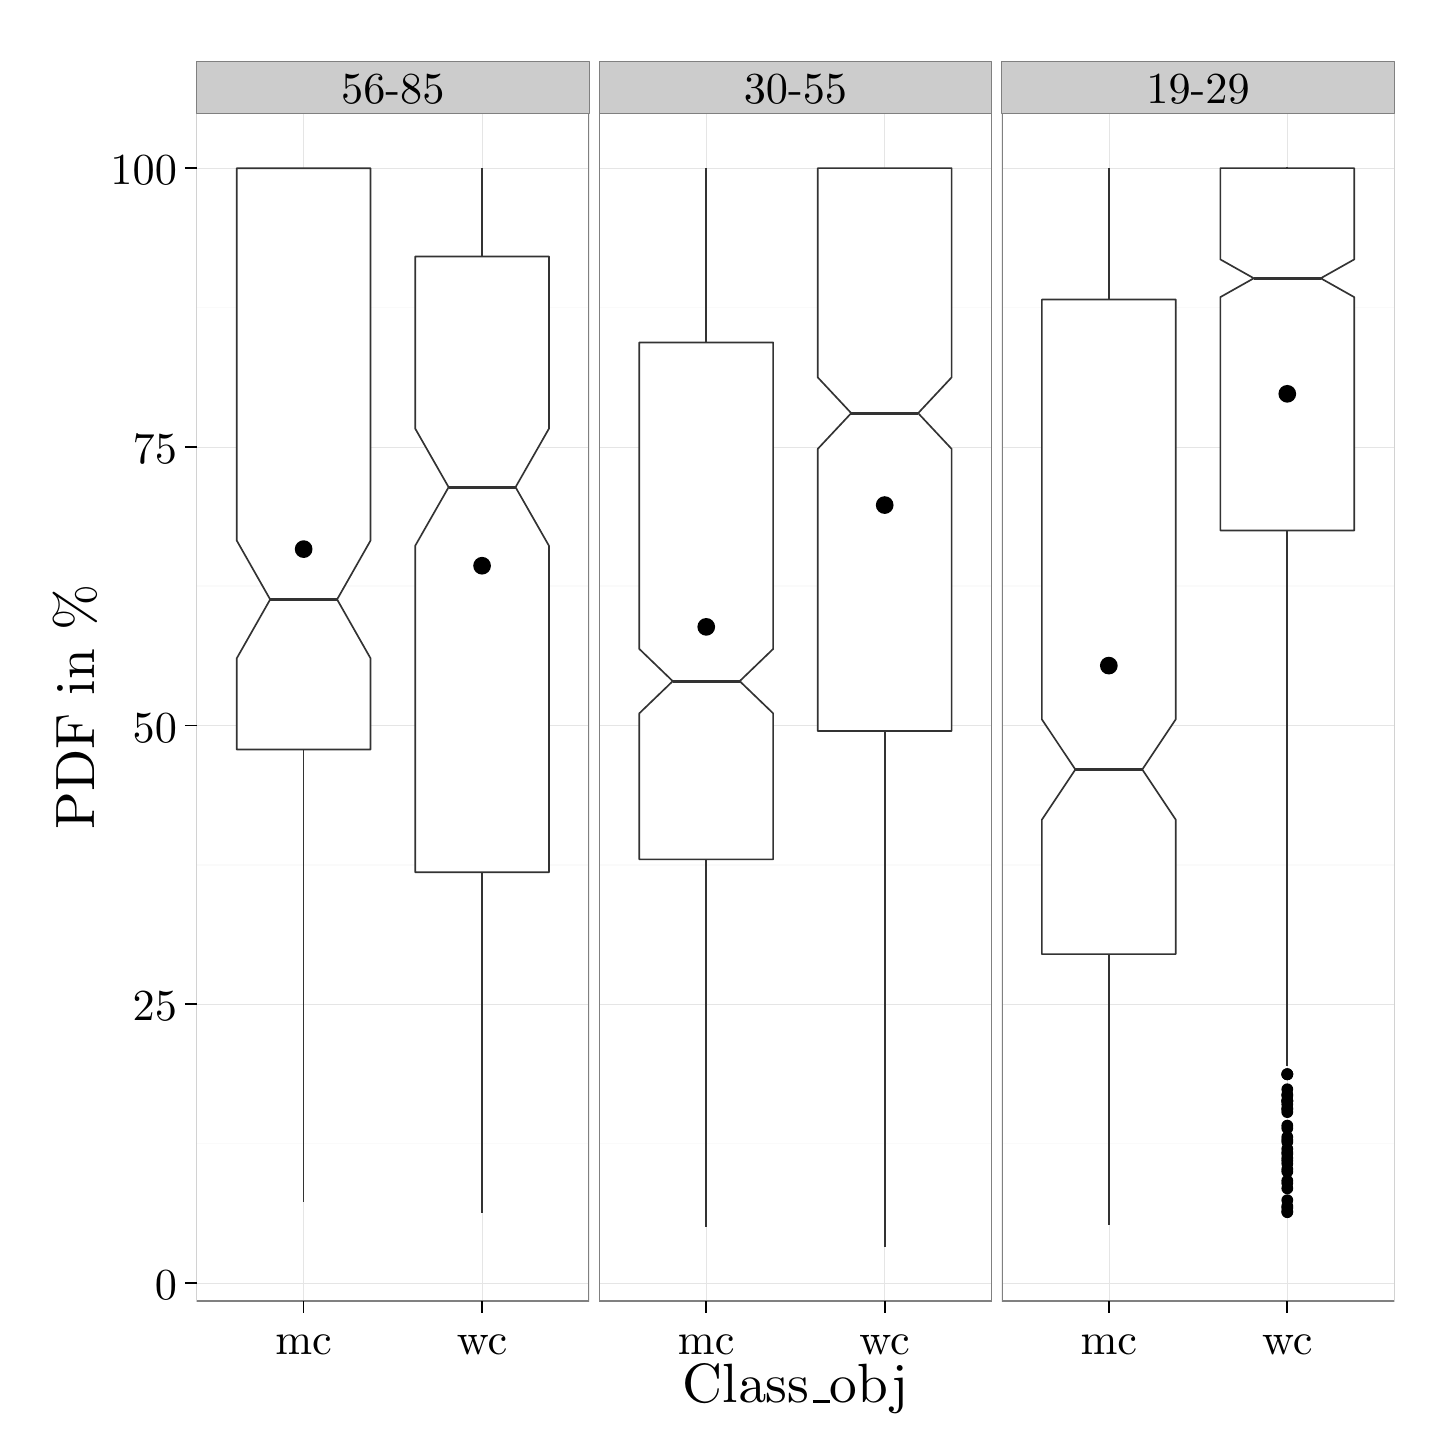
\begin{tikzpicture}[x=1pt,y=1pt]
\definecolor{fillColor}{RGB}{255,255,255}
\path[use as bounding box,fill=fillColor,fill opacity=0.00] (0,0) rectangle (505.89,505.89);
\begin{scope}
\path[clip] (  0.00,  0.00) rectangle (505.89,505.89);
\definecolor{drawColor}{RGB}{255,255,255}
\definecolor{fillColor}{RGB}{255,255,255}

\path[draw=drawColor,line width= 0.6pt,line join=round,line cap=round,fill=fillColor] (  0.00, -0.00) rectangle (505.89,505.89);
\end{scope}
\begin{scope}
\path[clip] ( 61.03, 45.77) rectangle (202.89,475.09);
\definecolor{fillColor}{RGB}{255,255,255}

\path[fill=fillColor] ( 61.03, 45.77) rectangle (202.89,475.09);
\definecolor{drawColor}{gray}{0.98}

\path[draw=drawColor,line width= 0.6pt,line join=round] ( 61.03,102.67) --
	(202.89,102.67);

\path[draw=drawColor,line width= 0.6pt,line join=round] ( 61.03,203.37) --
	(202.89,203.37);

\path[draw=drawColor,line width= 0.6pt,line join=round] ( 61.03,304.07) --
	(202.89,304.07);

\path[draw=drawColor,line width= 0.6pt,line join=round] ( 61.03,404.78) --
	(202.89,404.78);
\definecolor{drawColor}{gray}{0.90}

\path[draw=drawColor,line width= 0.2pt,line join=round] ( 61.03, 52.32) --
	(202.89, 52.32);

\path[draw=drawColor,line width= 0.2pt,line join=round] ( 61.03,153.02) --
	(202.89,153.02);

\path[draw=drawColor,line width= 0.2pt,line join=round] ( 61.03,253.72) --
	(202.89,253.72);

\path[draw=drawColor,line width= 0.2pt,line join=round] ( 61.03,354.43) --
	(202.89,354.43);

\path[draw=drawColor,line width= 0.2pt,line join=round] ( 61.03,455.13) --
	(202.89,455.13);

\path[draw=drawColor,line width= 0.2pt,line join=round] ( 99.72, 45.77) --
	( 99.72,475.09);

\path[draw=drawColor,line width= 0.2pt,line join=round] (164.20, 45.77) --
	(164.20,475.09);
\definecolor{drawColor}{gray}{0.20}

\path[draw=drawColor,line width= 0.6pt,line join=round] ( 99.72,455.07) -- ( 99.72,455.13);

\path[draw=drawColor,line width= 0.6pt,line join=round] ( 99.72,245.04) -- ( 99.72, 81.64);

\path[draw=drawColor,line width= 0.6pt,line join=round,line cap=round,fill=fillColor] ( 75.54,455.07) --
	( 75.54,320.57) --
	( 87.63,299.28) --
	( 75.54,277.99) --
	( 75.54,245.04) --
	(123.90,245.04) --
	(123.90,277.99) --
	(111.81,299.28) --
	(123.90,320.57) --
	(123.90,455.07) --
	( 75.54,455.07) --
	cycle;

\path[draw=drawColor,line width= 1.1pt,line join=round] ( 87.63,299.28) -- (111.81,299.28);

\path[draw=drawColor,line width= 0.6pt,line join=round] (164.20,423.21) -- (164.20,455.13);

\path[draw=drawColor,line width= 0.6pt,line join=round] (164.20,200.71) -- (164.20, 77.57);

\path[draw=drawColor,line width= 0.6pt,line join=round,line cap=round,fill=fillColor] (140.02,423.21) --
	(140.02,361.04) --
	(152.11,339.84) --
	(140.02,318.65) --
	(140.02,200.71) --
	(188.38,200.71) --
	(188.38,318.65) --
	(176.29,339.84) --
	(188.38,361.04) --
	(188.38,423.21) --
	(140.02,423.21) --
	cycle;

\path[draw=drawColor,line width= 1.1pt,line join=round] (152.11,339.84) -- (176.29,339.84);
\definecolor{fillColor}{RGB}{0,0,0}

\path[fill=fillColor] ( 99.72,317.46) circle (  3.20);

\path[fill=fillColor] (164.20,311.46) circle (  3.20);
\definecolor{drawColor}{gray}{0.50}

\path[draw=drawColor,line width= 0.6pt,line join=round,line cap=round] ( 61.03, 45.77) rectangle (202.89,475.09);
\end{scope}
\begin{scope}
\path[clip] (206.51, 45.77) rectangle (348.37,475.09);
\definecolor{fillColor}{RGB}{255,255,255}

\path[fill=fillColor] (206.51, 45.77) rectangle (348.37,475.09);
\definecolor{drawColor}{gray}{0.98}

\path[draw=drawColor,line width= 0.6pt,line join=round] (206.51,102.67) --
	(348.37,102.67);

\path[draw=drawColor,line width= 0.6pt,line join=round] (206.51,203.37) --
	(348.37,203.37);

\path[draw=drawColor,line width= 0.6pt,line join=round] (206.51,304.07) --
	(348.37,304.07);

\path[draw=drawColor,line width= 0.6pt,line join=round] (206.51,404.78) --
	(348.37,404.78);
\definecolor{drawColor}{gray}{0.90}

\path[draw=drawColor,line width= 0.2pt,line join=round] (206.51, 52.32) --
	(348.37, 52.32);

\path[draw=drawColor,line width= 0.2pt,line join=round] (206.51,153.02) --
	(348.37,153.02);

\path[draw=drawColor,line width= 0.2pt,line join=round] (206.51,253.72) --
	(348.37,253.72);

\path[draw=drawColor,line width= 0.2pt,line join=round] (206.51,354.43) --
	(348.37,354.43);

\path[draw=drawColor,line width= 0.2pt,line join=round] (206.51,455.13) --
	(348.37,455.13);

\path[draw=drawColor,line width= 0.2pt,line join=round] (245.20, 45.77) --
	(245.20,475.09);

\path[draw=drawColor,line width= 0.2pt,line join=round] (309.68, 45.77) --
	(309.68,475.09);
\definecolor{drawColor}{gray}{0.20}

\path[draw=drawColor,line width= 0.6pt,line join=round] (245.20,392.13) -- (245.20,455.13);

\path[draw=drawColor,line width= 0.6pt,line join=round] (245.20,205.34) -- (245.20, 72.66);

\path[draw=drawColor,line width= 0.6pt,line join=round,line cap=round,fill=fillColor] (221.01,392.13) --
	(221.01,281.39) --
	(233.10,269.75) --
	(221.01,258.12) --
	(221.01,205.34) --
	(269.38,205.34) --
	(269.38,258.12) --
	(257.29,269.75) --
	(269.38,281.39) --
	(269.38,392.13) --
	(221.01,392.13) --
	cycle;

\path[draw=drawColor,line width= 1.1pt,line join=round] (233.10,269.75) -- (257.29,269.75);

\path[draw=drawColor,line width= 0.6pt,line join=round] (309.68,455.13) -- (309.68,455.13);

\path[draw=drawColor,line width= 0.6pt,line join=round] (309.68,251.75) -- (309.68, 65.29);

\path[draw=drawColor,line width= 0.6pt,line join=round,line cap=round,fill=fillColor] (285.50,455.13) --
	(285.50,379.51) --
	(297.59,366.59) --
	(285.50,353.68) --
	(285.50,251.75) --
	(333.86,251.75) --
	(333.86,353.68) --
	(321.77,366.59) --
	(333.86,379.51) --
	(333.86,455.13) --
	(285.50,455.13) --
	cycle;

\path[draw=drawColor,line width= 1.1pt,line join=round] (297.59,366.59) -- (321.77,366.59);
\definecolor{fillColor}{RGB}{0,0,0}

\path[fill=fillColor] (245.20,289.37) circle (  3.20);

\path[fill=fillColor] (309.68,333.38) circle (  3.20);
\definecolor{drawColor}{gray}{0.50}

\path[draw=drawColor,line width= 0.6pt,line join=round,line cap=round] (206.51, 45.77) rectangle (348.37,475.09);
\end{scope}
\begin{scope}
\path[clip] (351.98, 45.77) rectangle (493.85,475.09);
\definecolor{fillColor}{RGB}{255,255,255}

\path[fill=fillColor] (351.98, 45.77) rectangle (493.85,475.09);
\definecolor{drawColor}{gray}{0.98}

\path[draw=drawColor,line width= 0.6pt,line join=round] (351.98,102.67) --
	(493.85,102.67);

\path[draw=drawColor,line width= 0.6pt,line join=round] (351.98,203.37) --
	(493.85,203.37);

\path[draw=drawColor,line width= 0.6pt,line join=round] (351.98,304.07) --
	(493.85,304.07);

\path[draw=drawColor,line width= 0.6pt,line join=round] (351.98,404.78) --
	(493.85,404.78);
\definecolor{drawColor}{gray}{0.90}

\path[draw=drawColor,line width= 0.2pt,line join=round] (351.98, 52.32) --
	(493.85, 52.32);

\path[draw=drawColor,line width= 0.2pt,line join=round] (351.98,153.02) --
	(493.85,153.02);

\path[draw=drawColor,line width= 0.2pt,line join=round] (351.98,253.72) --
	(493.85,253.72);

\path[draw=drawColor,line width= 0.2pt,line join=round] (351.98,354.43) --
	(493.85,354.43);

\path[draw=drawColor,line width= 0.2pt,line join=round] (351.98,455.13) --
	(493.85,455.13);

\path[draw=drawColor,line width= 0.2pt,line join=round] (390.67, 45.77) --
	(390.67,475.09);

\path[draw=drawColor,line width= 0.2pt,line join=round] (455.16, 45.77) --
	(455.16,475.09);
\definecolor{drawColor}{gray}{0.20}

\path[draw=drawColor,line width= 0.6pt,line join=round] (390.67,407.64) -- (390.67,455.13);

\path[draw=drawColor,line width= 0.6pt,line join=round] (390.67,171.11) -- (390.67, 73.10);

\path[draw=drawColor,line width= 0.6pt,line join=round,line cap=round,fill=fillColor] (366.49,407.64) --
	(366.49,255.94) --
	(378.58,237.81) --
	(366.49,219.68) --
	(366.49,171.11) --
	(414.85,171.11) --
	(414.85,219.68) --
	(402.76,237.81) --
	(414.85,255.94) --
	(414.85,407.64) --
	(366.49,407.64) --
	cycle;

\path[draw=drawColor,line width= 1.1pt,line join=round] (378.58,237.81) -- (402.76,237.81);
\definecolor{fillColor}{RGB}{0,0,0}

\path[fill=fillColor] (455.16,115.03) circle (  2.13);

\path[fill=fillColor] (455.16, 89.25) circle (  2.13);

\path[fill=fillColor] (455.16, 98.88) circle (  2.13);

\path[fill=fillColor] (455.16,119.99) circle (  2.13);

\path[fill=fillColor] (455.16,122.28) circle (  2.13);

\path[fill=fillColor] (455.16,108.19) circle (  2.13);

\path[fill=fillColor] (455.16,109.15) circle (  2.13);

\path[fill=fillColor] (455.16, 82.20) circle (  2.13);

\path[fill=fillColor] (455.16,114.03) circle (  2.13);

\path[fill=fillColor] (455.16, 77.85) circle (  2.13);

\path[fill=fillColor] (455.16, 99.53) circle (  2.13);

\path[fill=fillColor] (455.16, 92.52) circle (  2.13);

\path[fill=fillColor] (455.16,100.77) circle (  2.13);

\path[fill=fillColor] (455.16,117.97) circle (  2.13);

\path[fill=fillColor] (455.16, 96.50) circle (  2.13);

\path[fill=fillColor] (455.16,127.72) circle (  2.13);

\path[fill=fillColor] (455.16, 93.40) circle (  2.13);

\path[fill=fillColor] (455.16, 95.38) circle (  2.13);

\path[fill=fillColor] (455.16, 97.39) circle (  2.13);

\path[fill=fillColor] (455.16, 86.47) circle (  2.13);

\path[fill=fillColor] (455.16,127.68) circle (  2.13);

\path[fill=fillColor] (455.16,118.18) circle (  2.13);

\path[fill=fillColor] (455.16,115.36) circle (  2.13);

\path[fill=fillColor] (455.16, 88.33) circle (  2.13);

\path[fill=fillColor] (455.16, 80.03) circle (  2.13);

\path[fill=fillColor] (455.16,104.00) circle (  2.13);

\path[fill=fillColor] (455.16,116.85) circle (  2.13);

\path[fill=fillColor] (455.16, 79.43) circle (  2.13);

\path[fill=fillColor] (455.16,120.39) circle (  2.13);

\path[fill=fillColor] (455.16, 78.18) circle (  2.13);

\path[fill=fillColor] (455.16,105.04) circle (  2.13);

\path[fill=fillColor] (455.16,103.23) circle (  2.13);

\path[fill=fillColor] (455.16,118.06) circle (  2.13);

\path[fill=fillColor] (455.16,127.72) circle (  2.13);

\path[draw=drawColor,line width= 0.6pt,line join=round] (455.16,455.13) -- (455.16,455.57);

\path[draw=drawColor,line width= 0.6pt,line join=round] (455.16,324.19) -- (455.16,130.86);
\definecolor{fillColor}{RGB}{255,255,255}

\path[draw=drawColor,line width= 0.6pt,line join=round,line cap=round,fill=fillColor] (430.97,455.13) --
	(430.97,422.14) --
	(443.06,415.33) --
	(430.97,408.52) --
	(430.97,324.19) --
	(479.34,324.19) --
	(479.34,408.52) --
	(467.25,415.33) --
	(479.34,422.14) --
	(479.34,455.13) --
	(430.97,455.13) --
	cycle;

\path[draw=drawColor,line width= 1.1pt,line join=round] (443.06,415.33) -- (467.25,415.33);
\definecolor{fillColor}{RGB}{0,0,0}

\path[fill=fillColor] (390.67,275.37) circle (  3.20);

\path[fill=fillColor] (455.16,373.58) circle (  3.20);
\definecolor{drawColor}{gray}{0.50}

\path[draw=drawColor,line width= 0.6pt,line join=round,line cap=round] (351.98, 45.77) rectangle (493.85,475.09);
\end{scope}
\begin{scope}
\path[clip] (  0.00,  0.00) rectangle (505.89,505.89);
\definecolor{drawColor}{gray}{0.50}
\definecolor{fillColor}{gray}{0.80}

\path[draw=drawColor,line width= 0.2pt,line join=round,line cap=round,fill=fillColor] ( 61.03,475.09) rectangle (202.89,493.85);
\definecolor{drawColor}{RGB}{0,0,0}

\node[text=drawColor,anchor=base,inner sep=0pt, outer sep=0pt, scale=  1.60] at (131.96,478.43) {56-85};
\end{scope}
\begin{scope}
\path[clip] (  0.00,  0.00) rectangle (505.89,505.89);
\definecolor{drawColor}{gray}{0.50}
\definecolor{fillColor}{gray}{0.80}

\path[draw=drawColor,line width= 0.2pt,line join=round,line cap=round,fill=fillColor] (206.51,475.09) rectangle (348.37,493.85);
\definecolor{drawColor}{RGB}{0,0,0}

\node[text=drawColor,anchor=base,inner sep=0pt, outer sep=0pt, scale=  1.60] at (277.44,478.43) {30-55};
\end{scope}
\begin{scope}
\path[clip] (  0.00,  0.00) rectangle (505.89,505.89);
\definecolor{drawColor}{gray}{0.50}
\definecolor{fillColor}{gray}{0.80}

\path[draw=drawColor,line width= 0.2pt,line join=round,line cap=round,fill=fillColor] (351.98,475.09) rectangle (493.85,493.85);
\definecolor{drawColor}{RGB}{0,0,0}

\node[text=drawColor,anchor=base,inner sep=0pt, outer sep=0pt, scale=  1.60] at (422.91,478.43) {19-29};
\end{scope}
\begin{scope}
\path[clip] (  0.00,  0.00) rectangle (505.89,505.89);
\definecolor{drawColor}{RGB}{0,0,0}

\node[text=drawColor,anchor=base east,inner sep=0pt, outer sep=0pt, scale=  1.60] at ( 53.92, 46.28) {0};

\node[text=drawColor,anchor=base east,inner sep=0pt, outer sep=0pt, scale=  1.60] at ( 53.92,146.99) {25};

\node[text=drawColor,anchor=base east,inner sep=0pt, outer sep=0pt, scale=  1.60] at ( 53.92,247.69) {50};

\node[text=drawColor,anchor=base east,inner sep=0pt, outer sep=0pt, scale=  1.60] at ( 53.92,348.39) {75};

\node[text=drawColor,anchor=base east,inner sep=0pt, outer sep=0pt, scale=  1.60] at ( 53.92,449.10) {100};
\end{scope}
\begin{scope}
\path[clip] (  0.00,  0.00) rectangle (505.89,505.89);
\definecolor{drawColor}{RGB}{0,0,0}

\path[draw=drawColor,line width= 0.6pt,line join=round] ( 56.76, 52.32) --
	( 61.03, 52.32);

\path[draw=drawColor,line width= 0.6pt,line join=round] ( 56.76,153.02) --
	( 61.03,153.02);

\path[draw=drawColor,line width= 0.6pt,line join=round] ( 56.76,253.72) --
	( 61.03,253.72);

\path[draw=drawColor,line width= 0.6pt,line join=round] ( 56.76,354.43) --
	( 61.03,354.43);

\path[draw=drawColor,line width= 0.6pt,line join=round] ( 56.76,455.13) --
	( 61.03,455.13);
\end{scope}
\begin{scope}
\path[clip] (  0.00,  0.00) rectangle (505.89,505.89);
\definecolor{drawColor}{RGB}{0,0,0}

\path[draw=drawColor,line width= 0.6pt,line join=round] ( 99.72, 41.50) --
	( 99.72, 45.77);

\path[draw=drawColor,line width= 0.6pt,line join=round] (164.20, 41.50) --
	(164.20, 45.77);
\end{scope}
\begin{scope}
\path[clip] (  0.00,  0.00) rectangle (505.89,505.89);
\definecolor{drawColor}{RGB}{0,0,0}

\node[text=drawColor,anchor=base,inner sep=0pt, outer sep=0pt, scale=  1.60] at ( 99.72, 26.59) {mc};

\node[text=drawColor,anchor=base,inner sep=0pt, outer sep=0pt, scale=  1.60] at (164.20, 26.59) {wc};
\end{scope}
\begin{scope}
\path[clip] (  0.00,  0.00) rectangle (505.89,505.89);
\definecolor{drawColor}{RGB}{0,0,0}

\path[draw=drawColor,line width= 0.6pt,line join=round] (245.20, 41.50) --
	(245.20, 45.77);

\path[draw=drawColor,line width= 0.6pt,line join=round] (309.68, 41.50) --
	(309.68, 45.77);
\end{scope}
\begin{scope}
\path[clip] (  0.00,  0.00) rectangle (505.89,505.89);
\definecolor{drawColor}{RGB}{0,0,0}

\node[text=drawColor,anchor=base,inner sep=0pt, outer sep=0pt, scale=  1.60] at (245.20, 26.59) {mc};

\node[text=drawColor,anchor=base,inner sep=0pt, outer sep=0pt, scale=  1.60] at (309.68, 26.59) {wc};
\end{scope}
\begin{scope}
\path[clip] (  0.00,  0.00) rectangle (505.89,505.89);
\definecolor{drawColor}{RGB}{0,0,0}

\path[draw=drawColor,line width= 0.6pt,line join=round] (390.67, 41.50) --
	(390.67, 45.77);

\path[draw=drawColor,line width= 0.6pt,line join=round] (455.16, 41.50) --
	(455.16, 45.77);
\end{scope}
\begin{scope}
\path[clip] (  0.00,  0.00) rectangle (505.89,505.89);
\definecolor{drawColor}{RGB}{0,0,0}

\node[text=drawColor,anchor=base,inner sep=0pt, outer sep=0pt, scale=  1.60] at (390.67, 26.59) {mc};

\node[text=drawColor,anchor=base,inner sep=0pt, outer sep=0pt, scale=  1.60] at (455.16, 26.59) {wc};
\end{scope}
\begin{scope}
\path[clip] (  0.00,  0.00) rectangle (505.89,505.89);
\definecolor{drawColor}{RGB}{0,0,0}

\node[text=drawColor,anchor=base,inner sep=0pt, outer sep=0pt, scale=  2.00] at (277.44,  9.03) {Class{\_{}}obj};
\end{scope}
\begin{scope}
\path[clip] (  0.00,  0.00) rectangle (505.89,505.89);
\definecolor{drawColor}{RGB}{0,0,0}

\node[text=drawColor,rotate= 90.00,anchor=base,inner sep=0pt, outer sep=0pt, scale=  2.00] at ( 24.12,260.43) {PDF in {\%}};
\end{scope}
\end{tikzpicture}
} 
		\caption{box plot}
		\label{fig.box.k.ageclass}
	\end{subfigure}
	\begin{subfigure}{.49\textwidth}
		\centering
			\definecolor{shadecolor}{rgb}{0.969, 0.969, 0.969}
			\resizebox{\linewidth}{!}{% Created by tikzDevice version 0.8.1 on 2016-02-09 02:17:30
% !TEX encoding = UTF-8 Unicode
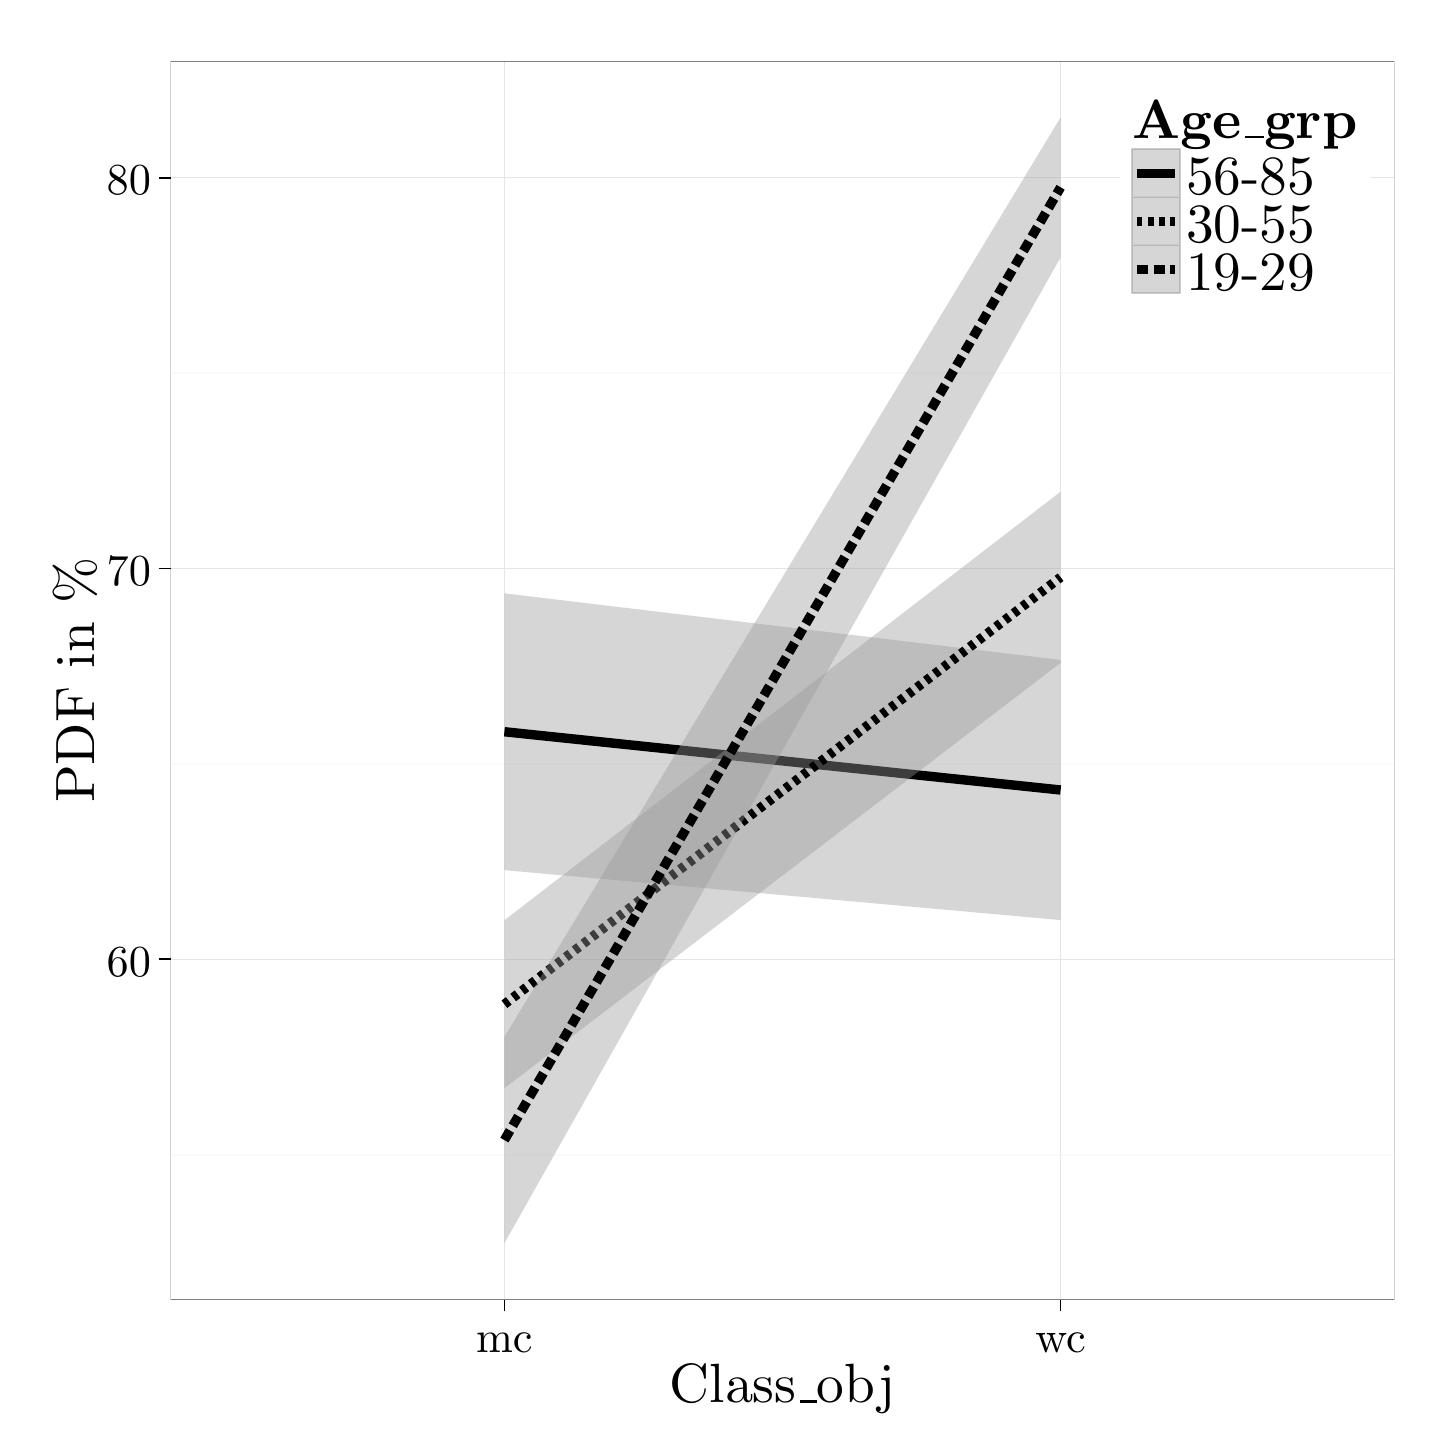
\begin{tikzpicture}[x=1pt,y=1pt]
\definecolor{fillColor}{RGB}{255,255,255}
\path[use as bounding box,fill=fillColor,fill opacity=0.00] (0,0) rectangle (505.89,505.89);
\begin{scope}
\path[clip] (  0.00,  0.00) rectangle (505.89,505.89);
\definecolor{drawColor}{RGB}{255,255,255}
\definecolor{fillColor}{RGB}{255,255,255}

\path[draw=drawColor,line width= 0.6pt,line join=round,line cap=round,fill=fillColor] (  0.00, -0.00) rectangle (505.89,505.89);
\end{scope}
\begin{scope}
\path[clip] ( 51.66, 46.31) rectangle (493.85,493.84);
\definecolor{fillColor}{RGB}{255,255,255}

\path[fill=fillColor] ( 51.66, 46.31) rectangle (493.84,493.84);
\definecolor{drawColor}{gray}{0.98}

\path[draw=drawColor,line width= 0.6pt,line join=round] ( 51.66, 98.63) --
	(493.85, 98.63);

\path[draw=drawColor,line width= 0.6pt,line join=round] ( 51.66,239.84) --
	(493.85,239.84);

\path[draw=drawColor,line width= 0.6pt,line join=round] ( 51.66,381.06) --
	(493.85,381.06);
\definecolor{drawColor}{gray}{0.90}

\path[draw=drawColor,line width= 0.2pt,line join=round] ( 51.66,169.24) --
	(493.85,169.24);

\path[draw=drawColor,line width= 0.2pt,line join=round] ( 51.66,310.45) --
	(493.85,310.45);

\path[draw=drawColor,line width= 0.2pt,line join=round] ( 51.66,451.67) --
	(493.85,451.67);

\path[draw=drawColor,line width= 0.2pt,line join=round] (172.26, 46.31) --
	(172.26,493.84);

\path[draw=drawColor,line width= 0.2pt,line join=round] (373.25, 46.31) --
	(373.25,493.84);
\definecolor{fillColor}{RGB}{153,153,153}

\path[fill=fillColor,fill opacity=0.40] (172.26,301.48) --
	(373.25,277.43) --
	(373.25,183.42) --
	(172.26,201.46) --
	cycle;
\definecolor{drawColor}{RGB}{0,0,0}

\path[draw=drawColor,line width= 3.4pt,line join=round] (172.26,251.47) --
	(373.25,230.42);

\path[fill=fillColor,fill opacity=0.40] (172.26,183.35) --
	(373.25,338.22) --
	(373.25,276.37) --
	(172.26,122.66) --
	cycle;

\path[draw=drawColor,line width= 3.4pt,dash pattern=on 2pt off 2pt ,line join=round] (172.26,153.00) --
	(373.25,307.30);

\path[fill=fillColor,fill opacity=0.40] (172.26,141.20) --
	(373.25,473.50) --
	(373.25,422.89) --
	(172.26, 66.65) --
	cycle;

\path[draw=drawColor,line width= 3.4pt,dash pattern=on 4pt off 2pt ,line join=round] (172.26,103.92) --
	(373.25,448.20);
\definecolor{drawColor}{gray}{0.50}

\path[draw=drawColor,line width= 0.6pt,line join=round,line cap=round] ( 51.66, 46.31) rectangle (493.84,493.84);
\end{scope}
\begin{scope}
\path[clip] (  0.00,  0.00) rectangle (505.89,505.89);
\definecolor{drawColor}{RGB}{0,0,0}

\node[text=drawColor,anchor=base east,inner sep=0pt, outer sep=0pt, scale=  1.60] at ( 44.55,163.20) {60};

\node[text=drawColor,anchor=base east,inner sep=0pt, outer sep=0pt, scale=  1.60] at ( 44.55,304.42) {70};

\node[text=drawColor,anchor=base east,inner sep=0pt, outer sep=0pt, scale=  1.60] at ( 44.55,445.64) {80};
\end{scope}
\begin{scope}
\path[clip] (  0.00,  0.00) rectangle (505.89,505.89);
\definecolor{drawColor}{RGB}{0,0,0}

\path[draw=drawColor,line width= 0.6pt,line join=round] ( 47.39,169.24) --
	( 51.66,169.24);

\path[draw=drawColor,line width= 0.6pt,line join=round] ( 47.39,310.45) --
	( 51.66,310.45);

\path[draw=drawColor,line width= 0.6pt,line join=round] ( 47.39,451.67) --
	( 51.66,451.67);
\end{scope}
\begin{scope}
\path[clip] (  0.00,  0.00) rectangle (505.89,505.89);
\definecolor{drawColor}{RGB}{0,0,0}

\path[draw=drawColor,line width= 0.6pt,line join=round] (172.26, 42.04) --
	(172.26, 46.31);

\path[draw=drawColor,line width= 0.6pt,line join=round] (373.25, 42.04) --
	(373.25, 46.31);
\end{scope}
\begin{scope}
\path[clip] (  0.00,  0.00) rectangle (505.89,505.89);
\definecolor{drawColor}{RGB}{0,0,0}

\node[text=drawColor,anchor=base,inner sep=0pt, outer sep=0pt, scale=  1.60] at (172.26, 27.13) {mc};

\node[text=drawColor,anchor=base,inner sep=0pt, outer sep=0pt, scale=  1.60] at (373.25, 27.13) {wc};
\end{scope}
\begin{scope}
\path[clip] (  0.00,  0.00) rectangle (505.89,505.89);
\definecolor{drawColor}{RGB}{0,0,0}

\node[text=drawColor,anchor=base,inner sep=0pt, outer sep=0pt, scale=  2.00] at (272.75,  9.03) {Class{\_{}}obj};
\end{scope}
\begin{scope}
\path[clip] (  0.00,  0.00) rectangle (505.89,505.89);
\definecolor{drawColor}{RGB}{0,0,0}

\node[text=drawColor,rotate= 90.00,anchor=base,inner sep=0pt, outer sep=0pt, scale=  2.00] at ( 24.12,270.08) {PDF in {\%}};
\end{scope}
\begin{scope}
\path[clip] (  0.00,  0.00) rectangle (505.89,505.89);
\definecolor{fillColor}{RGB}{255,255,255}

\path[fill=fillColor] (394.82,405.66) rectangle (484.98,484.98);
\end{scope}
\begin{scope}
\path[clip] (  0.00,  0.00) rectangle (505.89,505.89);
\definecolor{drawColor}{RGB}{0,0,0}

\node[text=drawColor,anchor=base west,inner sep=0pt, outer sep=0pt, scale=  2.00] at (399.08,465.96) {\bfseries Age{\_{}}grp};
\end{scope}
\begin{scope}
\path[clip] (  0.00,  0.00) rectangle (505.89,505.89);
\definecolor{drawColor}{gray}{0.80}
\definecolor{fillColor}{RGB}{255,255,255}

\path[draw=drawColor,line width= 0.6pt,line join=round,line cap=round,fill=fillColor] (399.08,444.61) rectangle (416.43,461.96);
\end{scope}
\begin{scope}
\path[clip] (  0.00,  0.00) rectangle (505.89,505.89);
\definecolor{fillColor}{RGB}{153,153,153}

\path[fill=fillColor,fill opacity=0.40] (399.08,444.61) rectangle (416.43,461.96);
\definecolor{drawColor}{RGB}{0,0,0}

\path[draw=drawColor,line width= 3.4pt,line join=round] (400.82,453.29) -- (414.69,453.29);
\end{scope}
\begin{scope}
\path[clip] (  0.00,  0.00) rectangle (505.89,505.89);
\definecolor{drawColor}{gray}{0.80}
\definecolor{fillColor}{RGB}{255,255,255}

\path[draw=drawColor,line width= 0.6pt,line join=round,line cap=round,fill=fillColor] (399.08,427.27) rectangle (416.43,444.61);
\end{scope}
\begin{scope}
\path[clip] (  0.00,  0.00) rectangle (505.89,505.89);
\definecolor{fillColor}{RGB}{153,153,153}

\path[fill=fillColor,fill opacity=0.40] (399.08,427.27) rectangle (416.43,444.61);
\definecolor{drawColor}{RGB}{0,0,0}

\path[draw=drawColor,line width= 3.4pt,dash pattern=on 2pt off 2pt ,line join=round] (400.82,435.94) -- (414.69,435.94);
\end{scope}
\begin{scope}
\path[clip] (  0.00,  0.00) rectangle (505.89,505.89);
\definecolor{drawColor}{gray}{0.80}
\definecolor{fillColor}{RGB}{255,255,255}

\path[draw=drawColor,line width= 0.6pt,line join=round,line cap=round,fill=fillColor] (399.08,409.92) rectangle (416.43,427.27);
\end{scope}
\begin{scope}
\path[clip] (  0.00,  0.00) rectangle (505.89,505.89);
\definecolor{fillColor}{RGB}{153,153,153}

\path[fill=fillColor,fill opacity=0.40] (399.08,409.92) rectangle (416.43,427.27);
\definecolor{drawColor}{RGB}{0,0,0}

\path[draw=drawColor,line width= 3.4pt,dash pattern=on 4pt off 2pt ,line join=round] (400.82,418.60) -- (414.69,418.60);
\end{scope}
\begin{scope}
\path[clip] (  0.00,  0.00) rectangle (505.89,505.89);
\definecolor{drawColor}{RGB}{0,0,0}

\node[text=drawColor,anchor=base west,inner sep=0pt, outer sep=0pt, scale=  2.00] at (418.60,445.75) {56-85};
\end{scope}
\begin{scope}
\path[clip] (  0.00,  0.00) rectangle (505.89,505.89);
\definecolor{drawColor}{RGB}{0,0,0}

\node[text=drawColor,anchor=base west,inner sep=0pt, outer sep=0pt, scale=  2.00] at (418.60,428.40) {30-55};
\end{scope}
\begin{scope}
\path[clip] (  0.00,  0.00) rectangle (505.89,505.89);
\definecolor{drawColor}{RGB}{0,0,0}

\node[text=drawColor,anchor=base west,inner sep=0pt, outer sep=0pt, scale=  2.00] at (418.60,411.06) {19-29};
\end{scope}
\end{tikzpicture}
} 
		\caption{regression plot}
		\label{fig.scatter.k.ageclass}
	\end{subfigure}
	\caption{/k/: PDF by age and social class (released only)}
\end{figure}

A much more linear development is visible in the interaction of age and social class as it is represented in \figref{fig.box.k.ageclass} and \figref{fig.scatter.k.ageclass}.
If we look at the class distinction and restrict ourselves to the oldest speakers in the sample (rightmost panel of \figref{fig.box.k.ageclass}) we find that, even though the medians seem to be just about significantly different from each other (cf. the notches), the means (black dots) are virtually identical.
A t-test on the raw data confirms that the difference in /k/ realisation between middle- and working-class speakers is not statistically robust in the age group 56--85 (t(515.679) = 0.608, p = 0.544).
In the next generation (middle panel), things have already changed.
There is now a wider gap between both the medians (cf. the notches) and the means of the two classes.
Additionally, the interquartile ranges as visualised by the vertical extent of the boxes now overlap (slightly) less.
For this age group, working-class speakers have a significantly higher \isi{PDF} (and thus more Scouse /k/ realisations) than middle-class Liverpudlians (t(1253.101) = -6.982, p < 0.001).
This difference does not only persist, but actually becomes larger and even more pronounced for the youngest speakers: the gap between middle and workings class subjects widens (t(698.451) = -13.959, p < 0.001).
In terms of social class, the development that has taken place from the oldest to the youngest speakers investigated in this study can thus be described as one of divergence: Middle-class speakers become consistently \emph{less} Scouse (\isi{PDF} drops), whereas working-class speakers just as consistently become \emph{more} Scouse (\isi{PDF} rises) across three generations.

\begin{table}[h]
	\centering
	\caption{/k/: t-tests of age by social class}
	\label{tab.k.classage.pvalues}
	\begin{tabular}{lrrrrrr}
		\toprule
		test & \multicolumn{3}{c}{middle class} & \multicolumn{3}{c}{working class}\\
		& t & df & p & t & df & p\\
		\midrule
		old-middle & \ensuremath{-3.530} & 458.418 & < 0.001 & 2.550 & 499.045 & 0.011\\
		middle-young & \ensuremath{-1.863} & 817.297 & 0.063 & 7.025 & 1243.562 & < 0.001\\
		young-old & \ensuremath{-4.641} & 585.844 & < 0.001 & 7.719 & 403.276 & < 0.001\\			 
		\bottomrule
	\end{tabular}
\end{table}

This divergence can also be seen in \figref{fig.scatter.k.ageclass}, where the solid regression line (old speakers) is essentially flat, the dotted one (middle-aged) has a moderate positive slope (which indicates a rise in \isi{PDF} going from the middle to the working-class speakers), and the dashed line (young subjects) has a very steep positive slope -- suggesting that the class effect is in the same direction but more pronounced than in the middle group.
If we zoom in on the middle-class speakers, we find that \isi{PDF} is actually highest in the old group, and decreases towards the middle and the young interviewees. The last two groups are not significantly different from one another as the overlapping standard deviations in the regression plot (dark grey areas) suggest and the t-test reported in \tabref{tab.k.classage.pvalues} (`middle-young') confirms.
In this social class, speakers have thus become less Scouse from the oldest to the middle-aged speakers, and then remained on that level.
For working-class Liverpudlians, on the other hand, the order of age groups is completely reversed: Old speakers have a comparatively low estimated \isi{PDF}, subjects aged 30--55 are in the middle, and the youngest participants have a very high estimated \isi{PDF} of around 80.
T-tests on the raw data find all three age groups to be significantly different from one another (cf. \tabref{tab.k.classage.pvalues}), which means that, with respect to /k/, old working-class speakers are less Scouse than the middle-aged, who in turn use less lenition than the youngest speakers.

\subsection{Social class and gender}
\label{sec.prod.res.con.k.classgender}

\begin{figure}[h]
	\centering
	\begin{subfigure}{.49\textwidth}
		\centering
			\definecolor{shadecolor}{rgb}{0.969, 0.969, 0.969}
			\resizebox{\linewidth}{!}{% Created by tikzDevice version 0.8.1 on 2016-02-09 02:17:31
% !TEX encoding = UTF-8 Unicode
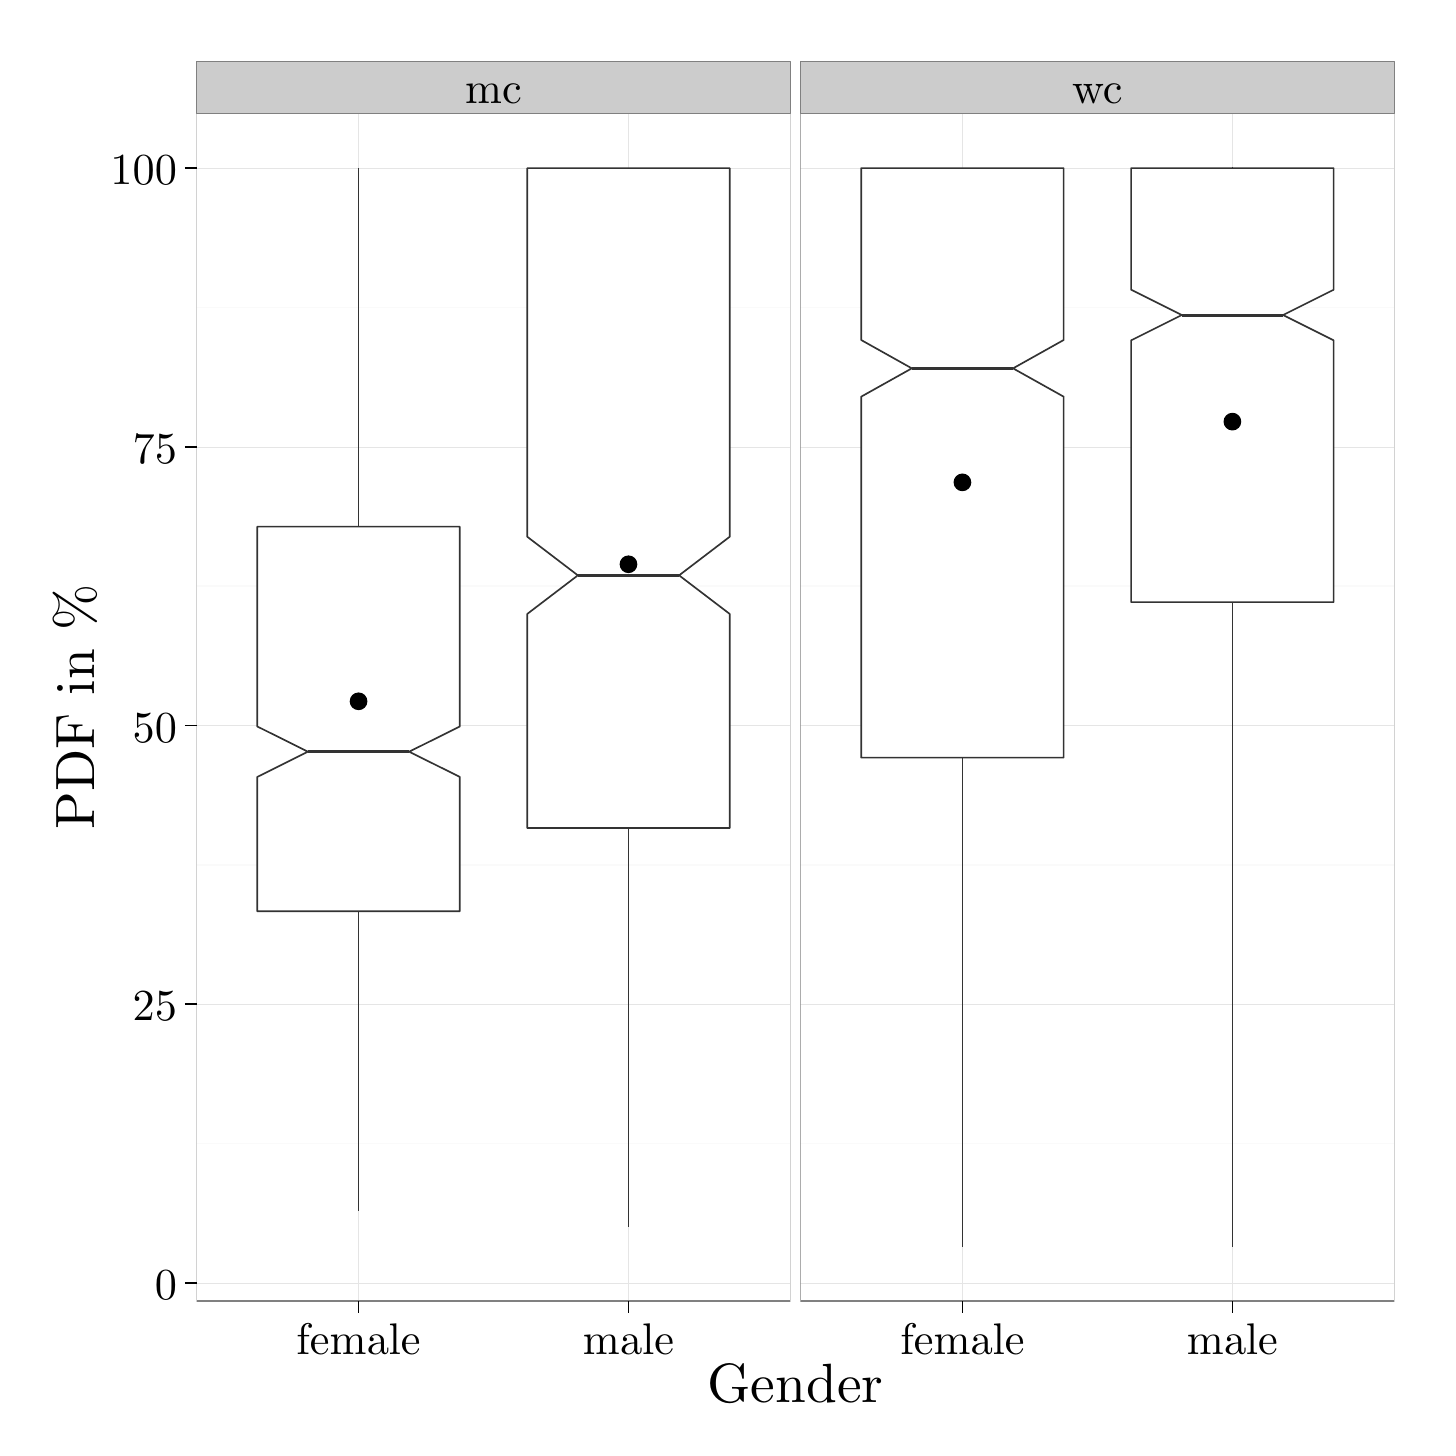
\begin{tikzpicture}[x=1pt,y=1pt]
\definecolor{fillColor}{RGB}{255,255,255}
\path[use as bounding box,fill=fillColor,fill opacity=0.00] (0,0) rectangle (505.89,505.89);
\begin{scope}
\path[clip] (  0.00,  0.00) rectangle (505.89,505.89);
\definecolor{drawColor}{RGB}{255,255,255}
\definecolor{fillColor}{RGB}{255,255,255}

\path[draw=drawColor,line width= 0.6pt,line join=round,line cap=round,fill=fillColor] (  0.00, -0.00) rectangle (505.89,505.89);
\end{scope}
\begin{scope}
\path[clip] ( 61.03, 45.77) rectangle (275.63,475.09);
\definecolor{fillColor}{RGB}{255,255,255}

\path[fill=fillColor] ( 61.03, 45.77) rectangle (275.63,475.09);
\definecolor{drawColor}{gray}{0.98}

\path[draw=drawColor,line width= 0.6pt,line join=round] ( 61.03,102.67) --
	(275.63,102.67);

\path[draw=drawColor,line width= 0.6pt,line join=round] ( 61.03,203.37) --
	(275.63,203.37);

\path[draw=drawColor,line width= 0.6pt,line join=round] ( 61.03,304.07) --
	(275.63,304.07);

\path[draw=drawColor,line width= 0.6pt,line join=round] ( 61.03,404.78) --
	(275.63,404.78);
\definecolor{drawColor}{gray}{0.90}

\path[draw=drawColor,line width= 0.2pt,line join=round] ( 61.03, 52.32) --
	(275.63, 52.32);

\path[draw=drawColor,line width= 0.2pt,line join=round] ( 61.03,153.02) --
	(275.63,153.02);

\path[draw=drawColor,line width= 0.2pt,line join=round] ( 61.03,253.72) --
	(275.63,253.72);

\path[draw=drawColor,line width= 0.2pt,line join=round] ( 61.03,354.43) --
	(275.63,354.43);

\path[draw=drawColor,line width= 0.2pt,line join=round] ( 61.03,455.13) --
	(275.63,455.13);

\path[draw=drawColor,line width= 0.2pt,line join=round] (119.56, 45.77) --
	(119.56,475.09);

\path[draw=drawColor,line width= 0.2pt,line join=round] (217.10, 45.77) --
	(217.10,475.09);
\definecolor{drawColor}{gray}{0.20}

\path[draw=drawColor,line width= 0.6pt,line join=round] (119.56,325.58) -- (119.56,455.13);

\path[draw=drawColor,line width= 0.6pt,line join=round] (119.56,186.61) -- (119.56, 78.22);

\path[draw=drawColor,line width= 0.6pt,line join=round,line cap=round,fill=fillColor] ( 82.98,325.58) --
	( 82.98,253.37) --
	(101.27,244.26) --
	( 82.98,235.15) --
	( 82.98,186.61) --
	(156.14,186.61) --
	(156.14,235.15) --
	(137.85,244.26) --
	(156.14,253.37) --
	(156.14,325.58) --
	( 82.98,325.58) --
	cycle;

\path[draw=drawColor,line width= 1.1pt,line join=round] (101.27,244.26) -- (137.85,244.26);

\path[draw=drawColor,line width= 0.6pt,line join=round] (217.10,455.13) -- (217.10,455.13);

\path[draw=drawColor,line width= 0.6pt,line join=round] (217.10,216.69) -- (217.10, 72.66);

\path[draw=drawColor,line width= 0.6pt,line join=round,line cap=round,fill=fillColor] (180.52,455.13) --
	(180.52,321.93) --
	(198.81,307.98) --
	(180.52,294.04) --
	(180.52,216.69) --
	(253.68,216.69) --
	(253.68,294.04) --
	(235.39,307.98) --
	(253.68,321.93) --
	(253.68,455.13) --
	(180.52,455.13) --
	cycle;

\path[draw=drawColor,line width= 1.1pt,line join=round] (198.81,307.98) -- (235.39,307.98);
\definecolor{fillColor}{RGB}{0,0,0}

\path[fill=fillColor] (119.56,262.47) circle (  3.20);

\path[fill=fillColor] (217.10,311.99) circle (  3.20);
\definecolor{drawColor}{gray}{0.50}

\path[draw=drawColor,line width= 0.6pt,line join=round,line cap=round] ( 61.03, 45.77) rectangle (275.63,475.09);
\end{scope}
\begin{scope}
\path[clip] (279.24, 45.77) rectangle (493.85,475.09);
\definecolor{fillColor}{RGB}{255,255,255}

\path[fill=fillColor] (279.24, 45.77) rectangle (493.85,475.09);
\definecolor{drawColor}{gray}{0.98}

\path[draw=drawColor,line width= 0.6pt,line join=round] (279.24,102.67) --
	(493.85,102.67);

\path[draw=drawColor,line width= 0.6pt,line join=round] (279.24,203.37) --
	(493.85,203.37);

\path[draw=drawColor,line width= 0.6pt,line join=round] (279.24,304.07) --
	(493.85,304.07);

\path[draw=drawColor,line width= 0.6pt,line join=round] (279.24,404.78) --
	(493.85,404.78);
\definecolor{drawColor}{gray}{0.90}

\path[draw=drawColor,line width= 0.2pt,line join=round] (279.24, 52.32) --
	(493.85, 52.32);

\path[draw=drawColor,line width= 0.2pt,line join=round] (279.24,153.02) --
	(493.85,153.02);

\path[draw=drawColor,line width= 0.2pt,line join=round] (279.24,253.72) --
	(493.85,253.72);

\path[draw=drawColor,line width= 0.2pt,line join=round] (279.24,354.43) --
	(493.85,354.43);

\path[draw=drawColor,line width= 0.2pt,line join=round] (279.24,455.13) --
	(493.85,455.13);

\path[draw=drawColor,line width= 0.2pt,line join=round] (337.77, 45.77) --
	(337.77,475.09);

\path[draw=drawColor,line width= 0.2pt,line join=round] (435.32, 45.77) --
	(435.32,475.09);
\definecolor{drawColor}{gray}{0.20}

\path[draw=drawColor,line width= 0.6pt,line join=round] (337.77,455.13) -- (337.77,455.13);

\path[draw=drawColor,line width= 0.6pt,line join=round] (337.77,242.12) -- (337.77, 65.29);

\path[draw=drawColor,line width= 0.6pt,line join=round,line cap=round,fill=fillColor] (301.19,455.13) --
	(301.19,393.02) --
	(319.48,382.78) --
	(301.19,372.55) --
	(301.19,242.12) --
	(374.35,242.12) --
	(374.35,372.55) --
	(356.06,382.78) --
	(374.35,393.02) --
	(374.35,455.13) --
	(301.19,455.13) --
	cycle;

\path[draw=drawColor,line width= 1.1pt,line join=round] (319.48,382.78) -- (356.06,382.78);

\path[draw=drawColor,line width= 0.6pt,line join=round] (435.32,455.13) -- (435.32,455.57);

\path[draw=drawColor,line width= 0.6pt,line join=round] (435.32,298.31) -- (435.32, 65.45);

\path[draw=drawColor,line width= 0.6pt,line join=round,line cap=round,fill=fillColor] (398.74,455.13) --
	(398.74,411.18) --
	(417.03,402.04) --
	(398.74,392.90) --
	(398.74,298.31) --
	(471.90,298.31) --
	(471.90,392.90) --
	(453.61,402.04) --
	(471.90,411.18) --
	(471.90,455.13) --
	(398.74,455.13) --
	cycle;

\path[draw=drawColor,line width= 1.1pt,line join=round] (417.03,402.04) -- (453.61,402.04);
\definecolor{fillColor}{RGB}{0,0,0}

\path[fill=fillColor] (337.77,341.59) circle (  3.20);

\path[fill=fillColor] (435.32,363.53) circle (  3.20);
\definecolor{drawColor}{gray}{0.50}

\path[draw=drawColor,line width= 0.6pt,line join=round,line cap=round] (279.24, 45.77) rectangle (493.85,475.09);
\end{scope}
\begin{scope}
\path[clip] (  0.00,  0.00) rectangle (505.89,505.89);
\definecolor{drawColor}{gray}{0.50}
\definecolor{fillColor}{gray}{0.80}

\path[draw=drawColor,line width= 0.2pt,line join=round,line cap=round,fill=fillColor] ( 61.03,475.09) rectangle (275.63,493.85);
\definecolor{drawColor}{RGB}{0,0,0}

\node[text=drawColor,anchor=base,inner sep=0pt, outer sep=0pt, scale=  1.60] at (168.33,478.43) {mc};
\end{scope}
\begin{scope}
\path[clip] (  0.00,  0.00) rectangle (505.89,505.89);
\definecolor{drawColor}{gray}{0.50}
\definecolor{fillColor}{gray}{0.80}

\path[draw=drawColor,line width= 0.2pt,line join=round,line cap=round,fill=fillColor] (279.24,475.09) rectangle (493.85,493.85);
\definecolor{drawColor}{RGB}{0,0,0}

\node[text=drawColor,anchor=base,inner sep=0pt, outer sep=0pt, scale=  1.60] at (386.54,478.43) {wc};
\end{scope}
\begin{scope}
\path[clip] (  0.00,  0.00) rectangle (505.89,505.89);
\definecolor{drawColor}{RGB}{0,0,0}

\node[text=drawColor,anchor=base east,inner sep=0pt, outer sep=0pt, scale=  1.60] at ( 53.92, 46.28) {0};

\node[text=drawColor,anchor=base east,inner sep=0pt, outer sep=0pt, scale=  1.60] at ( 53.92,146.99) {25};

\node[text=drawColor,anchor=base east,inner sep=0pt, outer sep=0pt, scale=  1.60] at ( 53.92,247.69) {50};

\node[text=drawColor,anchor=base east,inner sep=0pt, outer sep=0pt, scale=  1.60] at ( 53.92,348.39) {75};

\node[text=drawColor,anchor=base east,inner sep=0pt, outer sep=0pt, scale=  1.60] at ( 53.92,449.10) {100};
\end{scope}
\begin{scope}
\path[clip] (  0.00,  0.00) rectangle (505.89,505.89);
\definecolor{drawColor}{RGB}{0,0,0}

\path[draw=drawColor,line width= 0.6pt,line join=round] ( 56.76, 52.32) --
	( 61.03, 52.32);

\path[draw=drawColor,line width= 0.6pt,line join=round] ( 56.76,153.02) --
	( 61.03,153.02);

\path[draw=drawColor,line width= 0.6pt,line join=round] ( 56.76,253.72) --
	( 61.03,253.72);

\path[draw=drawColor,line width= 0.6pt,line join=round] ( 56.76,354.43) --
	( 61.03,354.43);

\path[draw=drawColor,line width= 0.6pt,line join=round] ( 56.76,455.13) --
	( 61.03,455.13);
\end{scope}
\begin{scope}
\path[clip] (  0.00,  0.00) rectangle (505.89,505.89);
\definecolor{drawColor}{RGB}{0,0,0}

\path[draw=drawColor,line width= 0.6pt,line join=round] (119.56, 41.50) --
	(119.56, 45.77);

\path[draw=drawColor,line width= 0.6pt,line join=round] (217.10, 41.50) --
	(217.10, 45.77);
\end{scope}
\begin{scope}
\path[clip] (  0.00,  0.00) rectangle (505.89,505.89);
\definecolor{drawColor}{RGB}{0,0,0}

\node[text=drawColor,anchor=base,inner sep=0pt, outer sep=0pt, scale=  1.60] at (119.56, 26.59) {female};

\node[text=drawColor,anchor=base,inner sep=0pt, outer sep=0pt, scale=  1.60] at (217.10, 26.59) {male};
\end{scope}
\begin{scope}
\path[clip] (  0.00,  0.00) rectangle (505.89,505.89);
\definecolor{drawColor}{RGB}{0,0,0}

\path[draw=drawColor,line width= 0.6pt,line join=round] (337.77, 41.50) --
	(337.77, 45.77);

\path[draw=drawColor,line width= 0.6pt,line join=round] (435.32, 41.50) --
	(435.32, 45.77);
\end{scope}
\begin{scope}
\path[clip] (  0.00,  0.00) rectangle (505.89,505.89);
\definecolor{drawColor}{RGB}{0,0,0}

\node[text=drawColor,anchor=base,inner sep=0pt, outer sep=0pt, scale=  1.60] at (337.77, 26.59) {female};

\node[text=drawColor,anchor=base,inner sep=0pt, outer sep=0pt, scale=  1.60] at (435.32, 26.59) {male};
\end{scope}
\begin{scope}
\path[clip] (  0.00,  0.00) rectangle (505.89,505.89);
\definecolor{drawColor}{RGB}{0,0,0}

\node[text=drawColor,anchor=base,inner sep=0pt, outer sep=0pt, scale=  2.00] at (277.44,  9.03) {Gender};
\end{scope}
\begin{scope}
\path[clip] (  0.00,  0.00) rectangle (505.89,505.89);
\definecolor{drawColor}{RGB}{0,0,0}

\node[text=drawColor,rotate= 90.00,anchor=base,inner sep=0pt, outer sep=0pt, scale=  2.00] at ( 24.12,260.43) {PDF in {\%}};
\end{scope}
\end{tikzpicture}
} 
		\caption{box plot}
		\label{fig.box.k.classgender}
	\end{subfigure}
	\begin{subfigure}{.49\textwidth}
		\centering
			\definecolor{shadecolor}{rgb}{0.969, 0.969, 0.969}
			\resizebox{\linewidth}{!}{% Created by tikzDevice version 0.8.1 on 2016-02-09 02:17:32
% !TEX encoding = UTF-8 Unicode
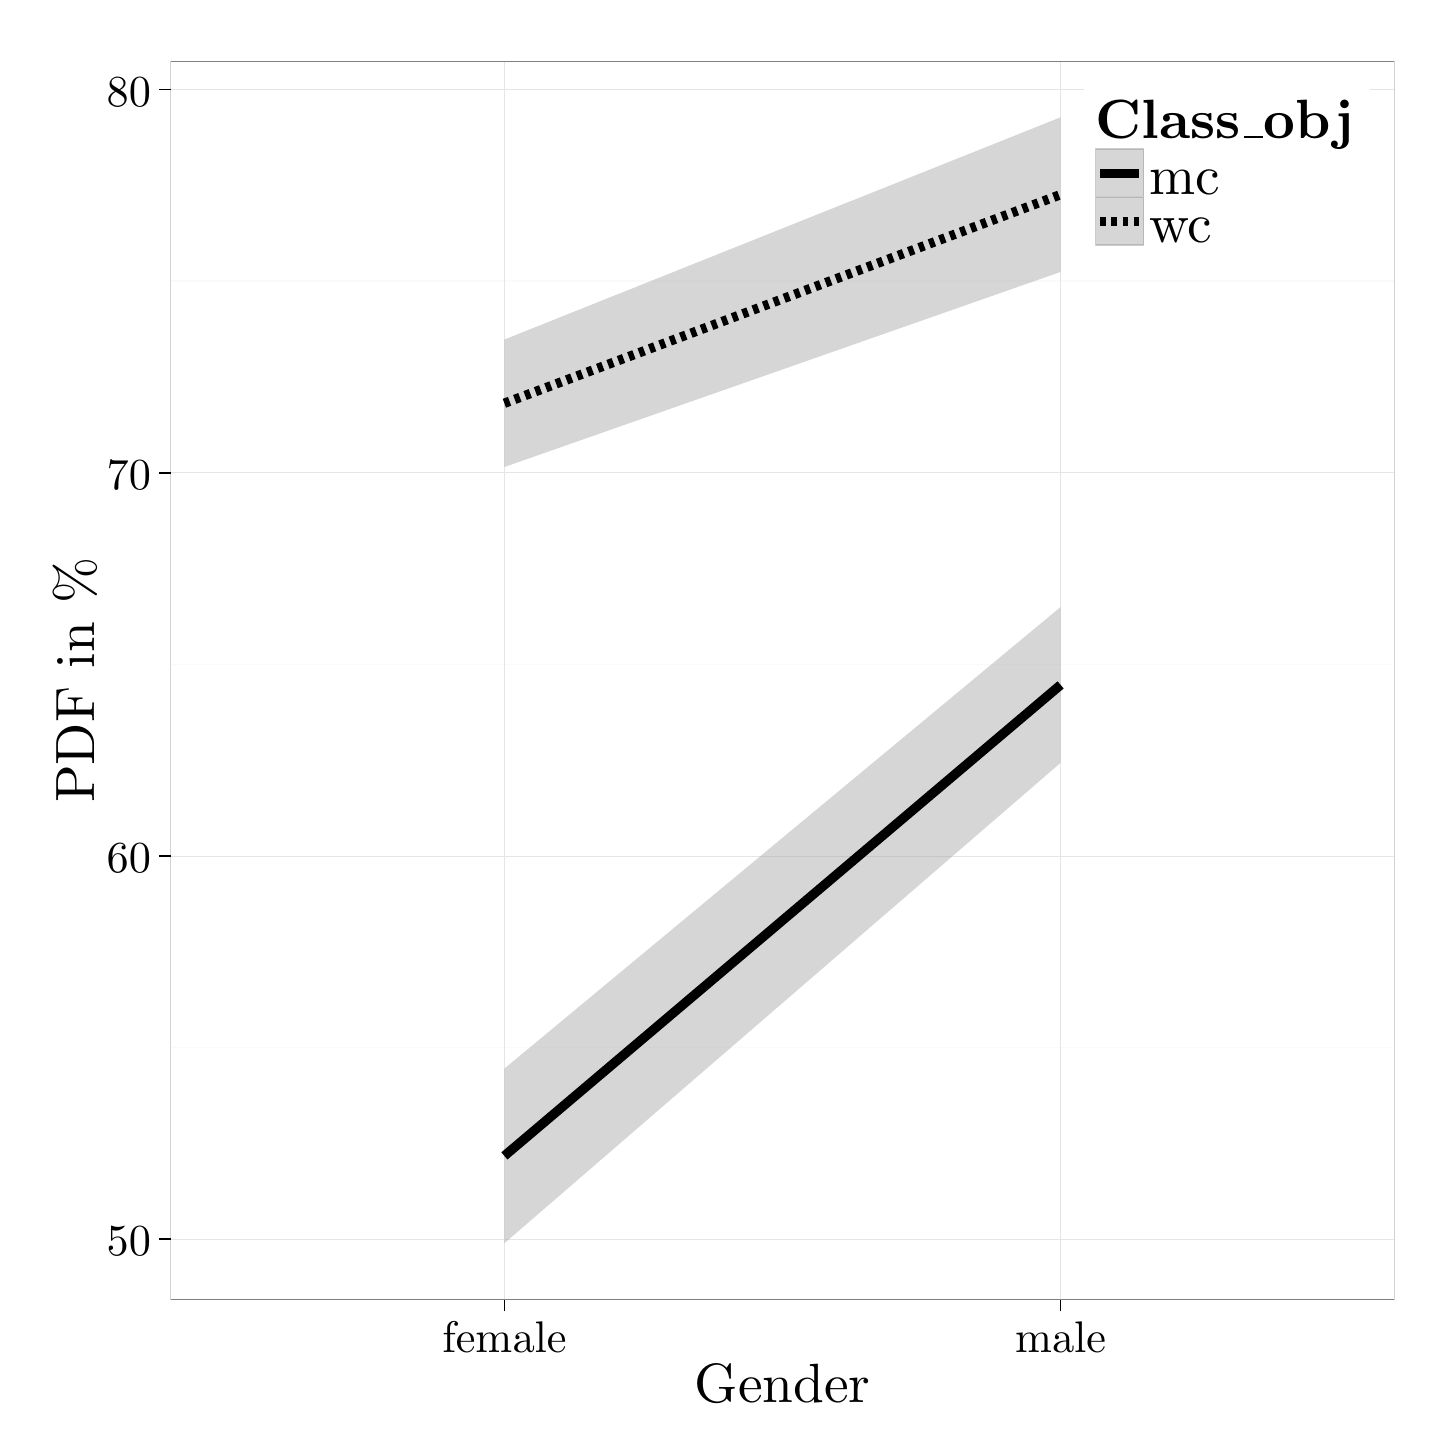
\begin{tikzpicture}[x=1pt,y=1pt]
\definecolor{fillColor}{RGB}{255,255,255}
\path[use as bounding box,fill=fillColor,fill opacity=0.00] (0,0) rectangle (505.89,505.89);
\begin{scope}
\path[clip] (  0.00,  0.00) rectangle (505.89,505.89);
\definecolor{drawColor}{RGB}{255,255,255}
\definecolor{fillColor}{RGB}{255,255,255}

\path[draw=drawColor,line width= 0.6pt,line join=round,line cap=round,fill=fillColor] (  0.00, -0.00) rectangle (505.89,505.89);
\end{scope}
\begin{scope}
\path[clip] ( 51.66, 46.31) rectangle (493.85,493.84);
\definecolor{fillColor}{RGB}{255,255,255}

\path[fill=fillColor] ( 51.66, 46.31) rectangle (493.84,493.84);
\definecolor{drawColor}{gray}{0.98}

\path[draw=drawColor,line width= 0.6pt,line join=round] ( 51.66,137.36) --
	(493.85,137.36);

\path[draw=drawColor,line width= 0.6pt,line join=round] ( 51.66,275.82) --
	(493.85,275.82);

\path[draw=drawColor,line width= 0.6pt,line join=round] ( 51.66,414.28) --
	(493.85,414.28);
\definecolor{drawColor}{gray}{0.90}

\path[draw=drawColor,line width= 0.2pt,line join=round] ( 51.66, 68.13) --
	(493.85, 68.13);

\path[draw=drawColor,line width= 0.2pt,line join=round] ( 51.66,206.59) --
	(493.85,206.59);

\path[draw=drawColor,line width= 0.2pt,line join=round] ( 51.66,345.05) --
	(493.85,345.05);

\path[draw=drawColor,line width= 0.2pt,line join=round] ( 51.66,483.51) --
	(493.85,483.51);

\path[draw=drawColor,line width= 0.2pt,line join=round] (172.26, 46.31) --
	(172.26,493.84);

\path[draw=drawColor,line width= 0.2pt,line join=round] (373.25, 46.31) --
	(373.25,493.84);
\definecolor{fillColor}{RGB}{153,153,153}

\path[fill=fillColor,fill opacity=0.40] (172.26,129.75) --
	(373.25,296.54) --
	(373.25,240.25) --
	(172.26, 66.65) --
	cycle;
\definecolor{drawColor}{RGB}{0,0,0}

\path[draw=drawColor,line width= 3.4pt,line join=round] (172.26, 98.20) --
	(373.25,268.40);

\path[fill=fillColor,fill opacity=0.40] (172.26,393.19) --
	(373.25,473.50) --
	(373.25,417.64) --
	(172.26,347.13) --
	cycle;

\path[draw=drawColor,line width= 3.4pt,dash pattern=on 2pt off 2pt ,line join=round] (172.26,370.16) --
	(373.25,445.57);
\definecolor{drawColor}{gray}{0.50}

\path[draw=drawColor,line width= 0.6pt,line join=round,line cap=round] ( 51.66, 46.31) rectangle (493.84,493.84);
\end{scope}
\begin{scope}
\path[clip] (  0.00,  0.00) rectangle (505.89,505.89);
\definecolor{drawColor}{RGB}{0,0,0}

\node[text=drawColor,anchor=base east,inner sep=0pt, outer sep=0pt, scale=  1.60] at ( 44.55, 62.09) {50};

\node[text=drawColor,anchor=base east,inner sep=0pt, outer sep=0pt, scale=  1.60] at ( 44.55,200.56) {60};

\node[text=drawColor,anchor=base east,inner sep=0pt, outer sep=0pt, scale=  1.60] at ( 44.55,339.02) {70};

\node[text=drawColor,anchor=base east,inner sep=0pt, outer sep=0pt, scale=  1.60] at ( 44.55,477.48) {80};
\end{scope}
\begin{scope}
\path[clip] (  0.00,  0.00) rectangle (505.89,505.89);
\definecolor{drawColor}{RGB}{0,0,0}

\path[draw=drawColor,line width= 0.6pt,line join=round] ( 47.39, 68.13) --
	( 51.66, 68.13);

\path[draw=drawColor,line width= 0.6pt,line join=round] ( 47.39,206.59) --
	( 51.66,206.59);

\path[draw=drawColor,line width= 0.6pt,line join=round] ( 47.39,345.05) --
	( 51.66,345.05);

\path[draw=drawColor,line width= 0.6pt,line join=round] ( 47.39,483.51) --
	( 51.66,483.51);
\end{scope}
\begin{scope}
\path[clip] (  0.00,  0.00) rectangle (505.89,505.89);
\definecolor{drawColor}{RGB}{0,0,0}

\path[draw=drawColor,line width= 0.6pt,line join=round] (172.26, 42.04) --
	(172.26, 46.31);

\path[draw=drawColor,line width= 0.6pt,line join=round] (373.25, 42.04) --
	(373.25, 46.31);
\end{scope}
\begin{scope}
\path[clip] (  0.00,  0.00) rectangle (505.89,505.89);
\definecolor{drawColor}{RGB}{0,0,0}

\node[text=drawColor,anchor=base,inner sep=0pt, outer sep=0pt, scale=  1.60] at (172.26, 27.13) {female};

\node[text=drawColor,anchor=base,inner sep=0pt, outer sep=0pt, scale=  1.60] at (373.25, 27.13) {male};
\end{scope}
\begin{scope}
\path[clip] (  0.00,  0.00) rectangle (505.89,505.89);
\definecolor{drawColor}{RGB}{0,0,0}

\node[text=drawColor,anchor=base,inner sep=0pt, outer sep=0pt, scale=  2.00] at (272.75,  9.03) {Gender};
\end{scope}
\begin{scope}
\path[clip] (  0.00,  0.00) rectangle (505.89,505.89);
\definecolor{drawColor}{RGB}{0,0,0}

\node[text=drawColor,rotate= 90.00,anchor=base,inner sep=0pt, outer sep=0pt, scale=  2.00] at ( 24.12,270.08) {PDF in {\%}};
\end{scope}
\begin{scope}
\path[clip] (  0.00,  0.00) rectangle (505.89,505.89);
\definecolor{fillColor}{RGB}{255,255,255}

\path[fill=fillColor] (381.61,423.00) rectangle (484.98,484.98);
\end{scope}
\begin{scope}
\path[clip] (  0.00,  0.00) rectangle (505.89,505.89);
\definecolor{drawColor}{RGB}{0,0,0}

\node[text=drawColor,anchor=base west,inner sep=0pt, outer sep=0pt, scale=  2.00] at (385.88,465.96) {\bfseries Class{\_{}}obj};
\end{scope}
\begin{scope}
\path[clip] (  0.00,  0.00) rectangle (505.89,505.89);
\definecolor{drawColor}{gray}{0.80}
\definecolor{fillColor}{RGB}{255,255,255}

\path[draw=drawColor,line width= 0.6pt,line join=round,line cap=round,fill=fillColor] (385.88,444.61) rectangle (403.22,461.96);
\end{scope}
\begin{scope}
\path[clip] (  0.00,  0.00) rectangle (505.89,505.89);
\definecolor{fillColor}{RGB}{153,153,153}

\path[fill=fillColor,fill opacity=0.40] (385.88,444.61) rectangle (403.22,461.96);
\definecolor{drawColor}{RGB}{0,0,0}

\path[draw=drawColor,line width= 3.4pt,line join=round] (387.61,453.29) -- (401.49,453.29);
\end{scope}
\begin{scope}
\path[clip] (  0.00,  0.00) rectangle (505.89,505.89);
\definecolor{drawColor}{gray}{0.80}
\definecolor{fillColor}{RGB}{255,255,255}

\path[draw=drawColor,line width= 0.6pt,line join=round,line cap=round,fill=fillColor] (385.88,427.27) rectangle (403.22,444.61);
\end{scope}
\begin{scope}
\path[clip] (  0.00,  0.00) rectangle (505.89,505.89);
\definecolor{fillColor}{RGB}{153,153,153}

\path[fill=fillColor,fill opacity=0.40] (385.88,427.27) rectangle (403.22,444.61);
\definecolor{drawColor}{RGB}{0,0,0}

\path[draw=drawColor,line width= 3.4pt,dash pattern=on 2pt off 2pt ,line join=round] (387.61,435.94) -- (401.49,435.94);
\end{scope}
\begin{scope}
\path[clip] (  0.00,  0.00) rectangle (505.89,505.89);
\definecolor{drawColor}{RGB}{0,0,0}

\node[text=drawColor,anchor=base west,inner sep=0pt, outer sep=0pt, scale=  2.00] at (405.39,445.75) {mc};
\end{scope}
\begin{scope}
\path[clip] (  0.00,  0.00) rectangle (505.89,505.89);
\definecolor{drawColor}{RGB}{0,0,0}

\node[text=drawColor,anchor=base west,inner sep=0pt, outer sep=0pt, scale=  2.00] at (405.39,428.40) {wc};
\end{scope}
\end{tikzpicture}
} 
		\caption{regression plot}
		\label{fig.scatter.k.classgender}
	\end{subfigure}
	\caption{/k/: PDF by gender and social class (released only)}
\end{figure}

Compared to the last two interactions (age X gender, and age X social class), the one of class and gender, albeit highly significant, is a lot less interesting.
Box plots (\figref{fig.box.k.classgender}) show that gender has roughly the same impact in both classes: men use more lenition than women.
This difference is significant in both the middle (t(1293.269) = -8.004, p < 0.001), and the working class (t(1709.667) = -4.196, p < 0.001), although the distance between women and men is smaller in the latter case.
If we take the opposite stance and look at class differences in the two genders separately, we end up with a very similar result.
The vertical distance of the regression lines shows that the difference in estimated \isi{PDF} between middle (solid line) and working class (dotted) is greater for female than for male speakers.
However, the effect is in the same direction (working-class speakers use more lenition than middle-class speakers), and it is highly significant for both women (t(1311.495) = -13.984, p < 0.001) \emph{and} men (t(1431.826) = -8.893, p < 0.001).
The nature of the class (gender) effect is thus essentially the same for both genders (social classes); there is only a difference in degree.

\subsection{Style shifting}
\label{sec.prod.res.con.k.shifting}

\begin{figure}[h]
	\centering
		\definecolor{shadecolor}{rgb}{0.969, 0.969, 0.969}
		\resizebox{0.5\linewidth}{!}{% Created by tikzDevice version 0.8.1 on 2016-02-09 02:17:35
% !TEX encoding = UTF-8 Unicode
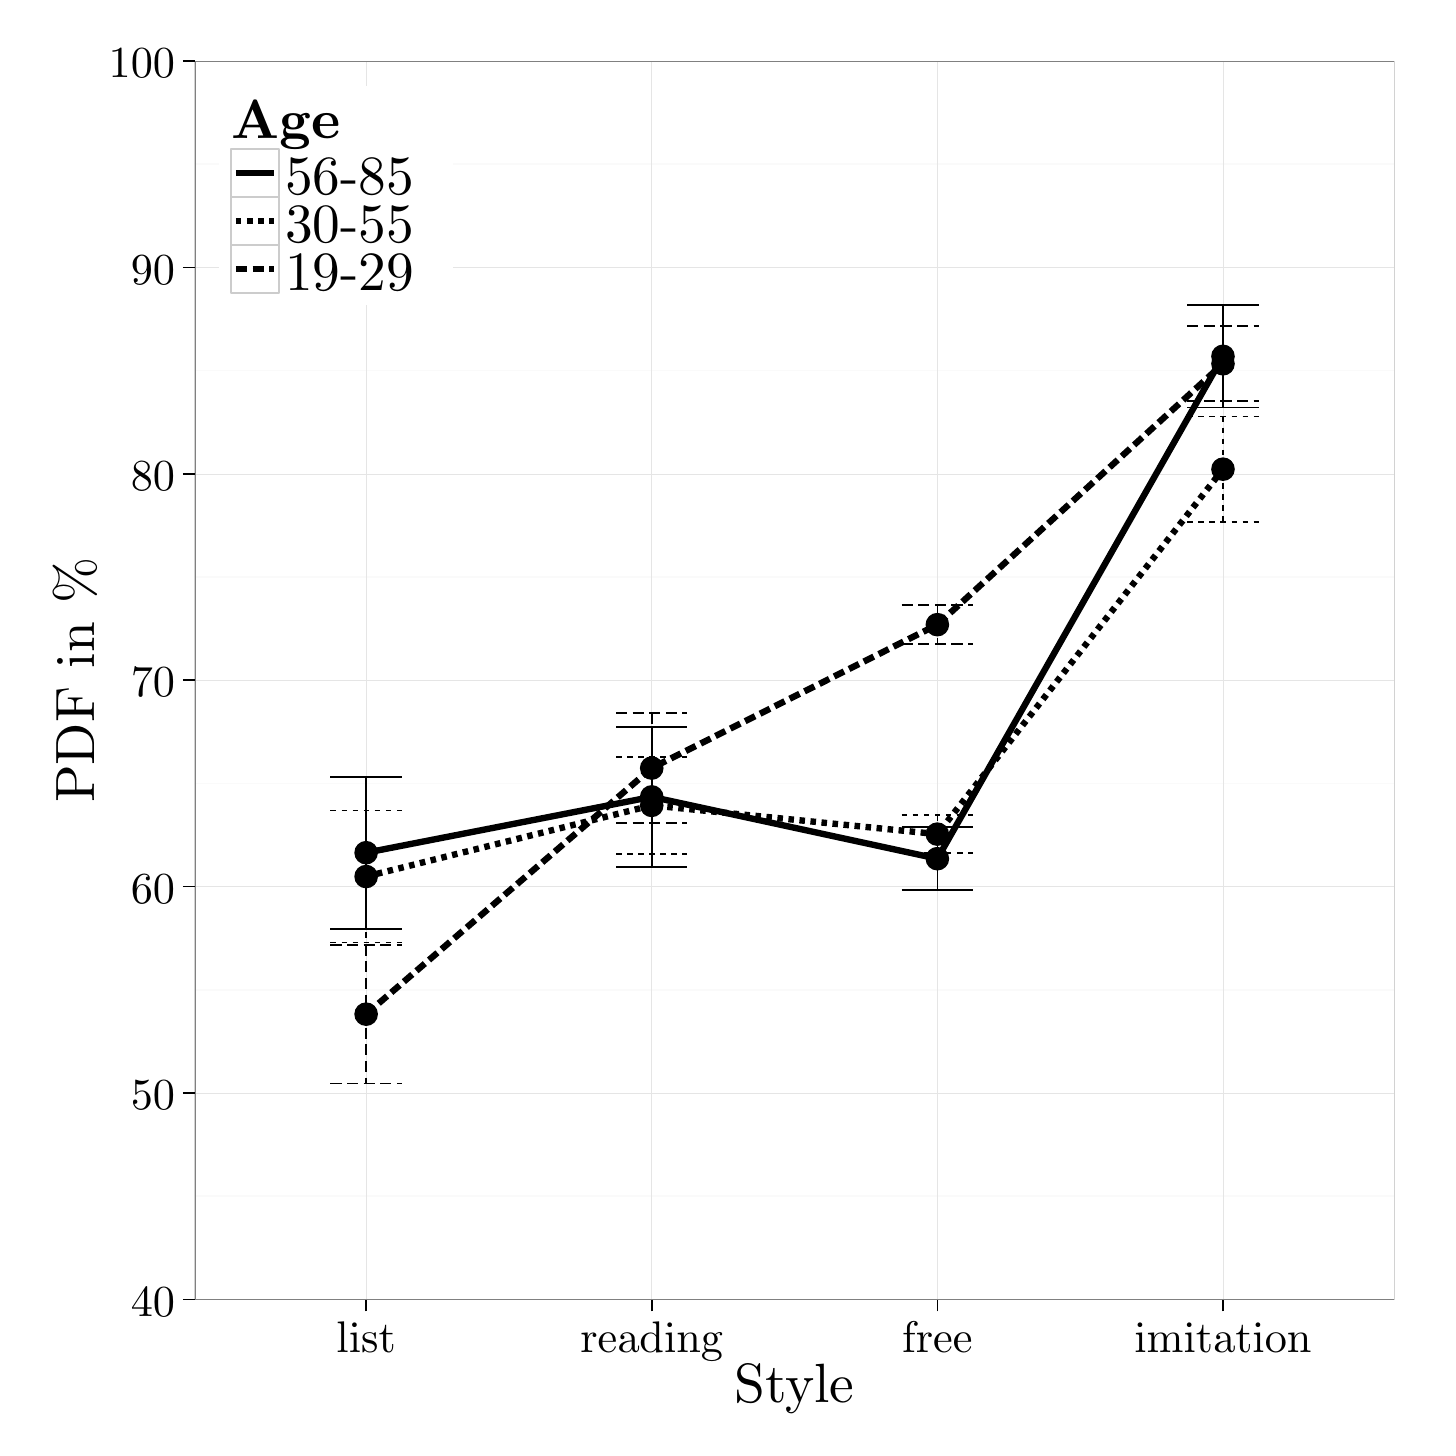
\begin{tikzpicture}[x=1pt,y=1pt]
\definecolor{fillColor}{RGB}{255,255,255}
\path[use as bounding box,fill=fillColor,fill opacity=0.00] (0,0) rectangle (505.89,505.89);
\begin{scope}
\path[clip] (  0.00,  0.00) rectangle (505.89,505.89);
\definecolor{drawColor}{RGB}{255,255,255}
\definecolor{fillColor}{RGB}{255,255,255}

\path[draw=drawColor,line width= 0.6pt,line join=round,line cap=round,fill=fillColor] (  0.00, -0.00) rectangle (505.89,505.89);
\end{scope}
\begin{scope}
\path[clip] ( 60.37, 46.31) rectangle (493.85,493.84);
\definecolor{fillColor}{RGB}{255,255,255}

\path[fill=fillColor] ( 60.37, 46.31) rectangle (493.85,493.84);
\definecolor{drawColor}{gray}{0.98}

\path[draw=drawColor,line width= 0.6pt,line join=round] ( 60.37, 83.60) --
	(493.85, 83.60);

\path[draw=drawColor,line width= 0.6pt,line join=round] ( 60.37,158.19) --
	(493.85,158.19);

\path[draw=drawColor,line width= 0.6pt,line join=round] ( 60.37,232.78) --
	(493.85,232.78);

\path[draw=drawColor,line width= 0.6pt,line join=round] ( 60.37,307.37) --
	(493.85,307.37);

\path[draw=drawColor,line width= 0.6pt,line join=round] ( 60.37,381.96) --
	(493.85,381.96);

\path[draw=drawColor,line width= 0.6pt,line join=round] ( 60.37,456.55) --
	(493.85,456.55);
\definecolor{drawColor}{gray}{0.90}

\path[draw=drawColor,line width= 0.2pt,line join=round] ( 60.37, 46.31) --
	(493.85, 46.31);

\path[draw=drawColor,line width= 0.2pt,line join=round] ( 60.37,120.90) --
	(493.85,120.90);

\path[draw=drawColor,line width= 0.2pt,line join=round] ( 60.37,195.49) --
	(493.85,195.49);

\path[draw=drawColor,line width= 0.2pt,line join=round] ( 60.37,270.08) --
	(493.85,270.08);

\path[draw=drawColor,line width= 0.2pt,line join=round] ( 60.37,344.67) --
	(493.85,344.67);

\path[draw=drawColor,line width= 0.2pt,line join=round] ( 60.37,419.26) --
	(493.85,419.26);

\path[draw=drawColor,line width= 0.2pt,line join=round] ( 60.37,493.84) --
	(493.85,493.84);

\path[draw=drawColor,line width= 0.2pt,line join=round] (122.30, 46.31) --
	(122.30,493.84);

\path[draw=drawColor,line width= 0.2pt,line join=round] (225.50, 46.31) --
	(225.50,493.84);

\path[draw=drawColor,line width= 0.2pt,line join=round] (328.71, 46.31) --
	(328.71,493.84);

\path[draw=drawColor,line width= 0.2pt,line join=round] (431.92, 46.31) --
	(431.92,493.84);
\definecolor{fillColor}{RGB}{0,0,0}

\path[fill=fillColor] (122.30,207.76) circle (  4.27);

\path[fill=fillColor] (122.30,199.15) circle (  4.27);

\path[fill=fillColor] (122.30,149.42) circle (  4.27);

\path[fill=fillColor] (225.50,227.93) circle (  4.27);

\path[fill=fillColor] (225.50,224.86) circle (  4.27);

\path[fill=fillColor] (225.50,238.34) circle (  4.27);

\path[fill=fillColor] (328.71,205.60) circle (  4.27);

\path[fill=fillColor] (328.71,214.47) circle (  4.27);

\path[fill=fillColor] (328.71,290.17) circle (  4.27);

\path[fill=fillColor] (431.92,387.13) circle (  4.27);

\path[fill=fillColor] (431.92,346.35) circle (  4.27);

\path[fill=fillColor] (431.92,384.44) circle (  4.27);
\definecolor{drawColor}{RGB}{0,0,0}

\path[draw=drawColor,line width= 2.3pt,line join=round] (122.30,207.76) --
	(225.50,227.93) --
	(328.71,205.60) --
	(431.92,387.13);

\path[draw=drawColor,line width= 2.3pt,dash pattern=on 2pt off 2pt ,line join=round] (122.30,199.15) --
	(225.50,224.86) --
	(328.71,214.47) --
	(431.92,346.35);

\path[draw=drawColor,line width= 2.3pt,dash pattern=on 4pt off 2pt ,line join=round] (122.30,149.42) --
	(225.50,238.34) --
	(328.71,290.17) --
	(431.92,384.44);

\path[draw=drawColor,line width= 0.6pt,line join=round] (109.40,235.21) --
	(135.20,235.21);

\path[draw=drawColor,line width= 0.6pt,line join=round] (122.30,235.21) --
	(122.30,180.30);

\path[draw=drawColor,line width= 0.6pt,line join=round] (109.40,180.30) --
	(135.20,180.30);

\path[draw=drawColor,line width= 0.6pt,line join=round] (212.60,253.17) --
	(238.41,253.17);

\path[draw=drawColor,line width= 0.6pt,line join=round] (225.50,253.17) --
	(225.50,202.69);

\path[draw=drawColor,line width= 0.6pt,line join=round] (212.60,202.69) --
	(238.41,202.69);

\path[draw=drawColor,line width= 0.6pt,line join=round] (315.81,217.04) --
	(341.61,217.04);

\path[draw=drawColor,line width= 0.6pt,line join=round] (328.71,217.04) --
	(328.71,194.17);

\path[draw=drawColor,line width= 0.6pt,line join=round] (315.81,194.17) --
	(341.61,194.17);

\path[draw=drawColor,line width= 0.6pt,line join=round] (419.02,405.62) --
	(444.82,405.62);

\path[draw=drawColor,line width= 0.6pt,line join=round] (431.92,405.62) --
	(431.92,368.63);

\path[draw=drawColor,line width= 0.6pt,line join=round] (419.02,368.63) --
	(444.82,368.63);

\path[draw=drawColor,line width= 0.6pt,dash pattern=on 2pt off 2pt ,line join=round] (109.40,222.98) --
	(135.20,222.98);

\path[draw=drawColor,line width= 0.6pt,dash pattern=on 2pt off 2pt ,line join=round] (122.30,222.98) --
	(122.30,175.32);

\path[draw=drawColor,line width= 0.6pt,dash pattern=on 2pt off 2pt ,line join=round] (109.40,175.32) --
	(135.20,175.32);

\path[draw=drawColor,line width= 0.6pt,dash pattern=on 2pt off 2pt ,line join=round] (212.60,242.44) --
	(238.41,242.44);

\path[draw=drawColor,line width= 0.6pt,dash pattern=on 2pt off 2pt ,line join=round] (225.50,242.44) --
	(225.50,207.29);

\path[draw=drawColor,line width= 0.6pt,dash pattern=on 2pt off 2pt ,line join=round] (212.60,207.29) --
	(238.41,207.29);

\path[draw=drawColor,line width= 0.6pt,dash pattern=on 2pt off 2pt ,line join=round] (315.81,221.30) --
	(341.61,221.30);

\path[draw=drawColor,line width= 0.6pt,dash pattern=on 2pt off 2pt ,line join=round] (328.71,221.30) --
	(328.71,207.65);

\path[draw=drawColor,line width= 0.6pt,dash pattern=on 2pt off 2pt ,line join=round] (315.81,207.65) --
	(341.61,207.65);

\path[draw=drawColor,line width= 0.6pt,dash pattern=on 2pt off 2pt ,line join=round] (419.02,365.36) --
	(444.82,365.36);

\path[draw=drawColor,line width= 0.6pt,dash pattern=on 2pt off 2pt ,line join=round] (431.92,365.36) --
	(431.92,327.34);

\path[draw=drawColor,line width= 0.6pt,dash pattern=on 2pt off 2pt ,line join=round] (419.02,327.34) --
	(444.82,327.34);

\path[draw=drawColor,line width= 0.6pt,dash pattern=on 4pt off 2pt ,line join=round] (109.40,174.49) --
	(135.20,174.49);

\path[draw=drawColor,line width= 0.6pt,dash pattern=on 4pt off 2pt ,line join=round] (122.30,174.49) --
	(122.30,124.36);

\path[draw=drawColor,line width= 0.6pt,dash pattern=on 4pt off 2pt ,line join=round] (109.40,124.36) --
	(135.20,124.36);

\path[draw=drawColor,line width= 0.6pt,dash pattern=on 4pt off 2pt ,line join=round] (212.60,258.14) --
	(238.41,258.14);

\path[draw=drawColor,line width= 0.6pt,dash pattern=on 4pt off 2pt ,line join=round] (225.50,258.14) --
	(225.50,218.54);

\path[draw=drawColor,line width= 0.6pt,dash pattern=on 4pt off 2pt ,line join=round] (212.60,218.54) --
	(238.41,218.54);

\path[draw=drawColor,line width= 0.6pt,dash pattern=on 4pt off 2pt ,line join=round] (315.81,297.24) --
	(341.61,297.24);

\path[draw=drawColor,line width= 0.6pt,dash pattern=on 4pt off 2pt ,line join=round] (328.71,297.24) --
	(328.71,283.11);

\path[draw=drawColor,line width= 0.6pt,dash pattern=on 4pt off 2pt ,line join=round] (315.81,283.11) --
	(341.61,283.11);

\path[draw=drawColor,line width= 0.6pt,dash pattern=on 4pt off 2pt ,line join=round] (419.02,398.00) --
	(444.82,398.00);

\path[draw=drawColor,line width= 0.6pt,dash pattern=on 4pt off 2pt ,line join=round] (431.92,398.00) --
	(431.92,370.88);

\path[draw=drawColor,line width= 0.6pt,dash pattern=on 4pt off 2pt ,line join=round] (419.02,370.88) --
	(444.82,370.88);
\definecolor{drawColor}{gray}{0.50}

\path[draw=drawColor,line width= 0.6pt,line join=round,line cap=round] ( 60.37, 46.31) rectangle (493.85,493.84);
\end{scope}
\begin{scope}
\path[clip] (  0.00,  0.00) rectangle (505.89,505.89);
\definecolor{drawColor}{RGB}{0,0,0}

\node[text=drawColor,anchor=base east,inner sep=0pt, outer sep=0pt, scale=  1.60] at ( 53.26, 40.27) {40};

\node[text=drawColor,anchor=base east,inner sep=0pt, outer sep=0pt, scale=  1.60] at ( 53.26,114.86) {50};

\node[text=drawColor,anchor=base east,inner sep=0pt, outer sep=0pt, scale=  1.60] at ( 53.26,189.45) {60};

\node[text=drawColor,anchor=base east,inner sep=0pt, outer sep=0pt, scale=  1.60] at ( 53.26,264.04) {70};

\node[text=drawColor,anchor=base east,inner sep=0pt, outer sep=0pt, scale=  1.60] at ( 53.26,338.63) {80};

\node[text=drawColor,anchor=base east,inner sep=0pt, outer sep=0pt, scale=  1.60] at ( 53.26,413.22) {90};

\node[text=drawColor,anchor=base east,inner sep=0pt, outer sep=0pt, scale=  1.60] at ( 53.26,487.81) {100};
\end{scope}
\begin{scope}
\path[clip] (  0.00,  0.00) rectangle (505.89,505.89);
\definecolor{drawColor}{RGB}{0,0,0}

\path[draw=drawColor,line width= 0.6pt,line join=round] ( 56.10, 46.31) --
	( 60.37, 46.31);

\path[draw=drawColor,line width= 0.6pt,line join=round] ( 56.10,120.90) --
	( 60.37,120.90);

\path[draw=drawColor,line width= 0.6pt,line join=round] ( 56.10,195.49) --
	( 60.37,195.49);

\path[draw=drawColor,line width= 0.6pt,line join=round] ( 56.10,270.08) --
	( 60.37,270.08);

\path[draw=drawColor,line width= 0.6pt,line join=round] ( 56.10,344.67) --
	( 60.37,344.67);

\path[draw=drawColor,line width= 0.6pt,line join=round] ( 56.10,419.26) --
	( 60.37,419.26);

\path[draw=drawColor,line width= 0.6pt,line join=round] ( 56.10,493.84) --
	( 60.37,493.84);
\end{scope}
\begin{scope}
\path[clip] (  0.00,  0.00) rectangle (505.89,505.89);
\definecolor{drawColor}{RGB}{0,0,0}

\path[draw=drawColor,line width= 0.6pt,line join=round] (122.30, 42.04) --
	(122.30, 46.31);

\path[draw=drawColor,line width= 0.6pt,line join=round] (225.50, 42.04) --
	(225.50, 46.31);

\path[draw=drawColor,line width= 0.6pt,line join=round] (328.71, 42.04) --
	(328.71, 46.31);

\path[draw=drawColor,line width= 0.6pt,line join=round] (431.92, 42.04) --
	(431.92, 46.31);
\end{scope}
\begin{scope}
\path[clip] (  0.00,  0.00) rectangle (505.89,505.89);
\definecolor{drawColor}{RGB}{0,0,0}

\node[text=drawColor,anchor=base,inner sep=0pt, outer sep=0pt, scale=  1.60] at (122.30, 27.13) {list};

\node[text=drawColor,anchor=base,inner sep=0pt, outer sep=0pt, scale=  1.60] at (225.50, 27.13) {reading};

\node[text=drawColor,anchor=base,inner sep=0pt, outer sep=0pt, scale=  1.60] at (328.71, 27.13) {free};

\node[text=drawColor,anchor=base,inner sep=0pt, outer sep=0pt, scale=  1.60] at (431.92, 27.13) {imitation};
\end{scope}
\begin{scope}
\path[clip] (  0.00,  0.00) rectangle (505.89,505.89);
\definecolor{drawColor}{RGB}{0,0,0}

\node[text=drawColor,anchor=base,inner sep=0pt, outer sep=0pt, scale=  2.00] at (277.11,  9.03) {Style};
\end{scope}
\begin{scope}
\path[clip] (  0.00,  0.00) rectangle (505.89,505.89);
\definecolor{drawColor}{RGB}{0,0,0}

\node[text=drawColor,rotate= 90.00,anchor=base,inner sep=0pt, outer sep=0pt, scale=  2.00] at ( 24.12,270.08) {PDF in {\%}};
\end{scope}
\begin{scope}
\path[clip] (  0.00,  0.00) rectangle (505.89,505.89);
\definecolor{fillColor}{RGB}{255,255,255}

\path[fill=fillColor] ( 69.24,405.66) rectangle (153.66,484.98);
\end{scope}
\begin{scope}
\path[clip] (  0.00,  0.00) rectangle (505.89,505.89);
\definecolor{drawColor}{RGB}{0,0,0}

\node[text=drawColor,anchor=base west,inner sep=0pt, outer sep=0pt, scale=  2.00] at ( 73.51,465.96) {\bfseries Age};
\end{scope}
\begin{scope}
\path[clip] (  0.00,  0.00) rectangle (505.89,505.89);
\definecolor{drawColor}{gray}{0.80}
\definecolor{fillColor}{RGB}{255,255,255}

\path[draw=drawColor,line width= 0.6pt,line join=round,line cap=round,fill=fillColor] ( 73.51,444.61) rectangle ( 90.85,461.96);
\end{scope}
\begin{scope}
\path[clip] (  0.00,  0.00) rectangle (505.89,505.89);
\definecolor{drawColor}{RGB}{0,0,0}

\path[draw=drawColor,line width= 2.3pt,line join=round] ( 75.24,453.29) -- ( 89.12,453.29);
\end{scope}
\begin{scope}
\path[clip] (  0.00,  0.00) rectangle (505.89,505.89);
\definecolor{drawColor}{RGB}{0,0,0}

\path[draw=drawColor,line width= 0.6pt,line join=round] ( 75.24,453.29) -- ( 89.12,453.29);
\end{scope}
\begin{scope}
\path[clip] (  0.00,  0.00) rectangle (505.89,505.89);
\definecolor{drawColor}{gray}{0.80}
\definecolor{fillColor}{RGB}{255,255,255}

\path[draw=drawColor,line width= 0.6pt,line join=round,line cap=round,fill=fillColor] ( 73.51,427.27) rectangle ( 90.85,444.61);
\end{scope}
\begin{scope}
\path[clip] (  0.00,  0.00) rectangle (505.89,505.89);
\definecolor{drawColor}{RGB}{0,0,0}

\path[draw=drawColor,line width= 2.3pt,dash pattern=on 2pt off 2pt ,line join=round] ( 75.24,435.94) -- ( 89.12,435.94);
\end{scope}
\begin{scope}
\path[clip] (  0.00,  0.00) rectangle (505.89,505.89);
\definecolor{drawColor}{RGB}{0,0,0}

\path[draw=drawColor,line width= 0.6pt,dash pattern=on 2pt off 2pt ,line join=round] ( 75.24,435.94) -- ( 89.12,435.94);
\end{scope}
\begin{scope}
\path[clip] (  0.00,  0.00) rectangle (505.89,505.89);
\definecolor{drawColor}{gray}{0.80}
\definecolor{fillColor}{RGB}{255,255,255}

\path[draw=drawColor,line width= 0.6pt,line join=round,line cap=round,fill=fillColor] ( 73.51,409.92) rectangle ( 90.85,427.27);
\end{scope}
\begin{scope}
\path[clip] (  0.00,  0.00) rectangle (505.89,505.89);
\definecolor{drawColor}{RGB}{0,0,0}

\path[draw=drawColor,line width= 2.3pt,dash pattern=on 4pt off 2pt ,line join=round] ( 75.24,418.60) -- ( 89.12,418.60);
\end{scope}
\begin{scope}
\path[clip] (  0.00,  0.00) rectangle (505.89,505.89);
\definecolor{drawColor}{RGB}{0,0,0}

\path[draw=drawColor,line width= 0.6pt,dash pattern=on 4pt off 2pt ,line join=round] ( 75.24,418.60) -- ( 89.12,418.60);
\end{scope}
\begin{scope}
\path[clip] (  0.00,  0.00) rectangle (505.89,505.89);
\definecolor{drawColor}{RGB}{0,0,0}

\node[text=drawColor,anchor=base west,inner sep=0pt, outer sep=0pt, scale=  2.00] at ( 93.02,445.75) {56-85};
\end{scope}
\begin{scope}
\path[clip] (  0.00,  0.00) rectangle (505.89,505.89);
\definecolor{drawColor}{RGB}{0,0,0}

\node[text=drawColor,anchor=base west,inner sep=0pt, outer sep=0pt, scale=  2.00] at ( 93.02,428.40) {30-55};
\end{scope}
\begin{scope}
\path[clip] (  0.00,  0.00) rectangle (505.89,505.89);
\definecolor{drawColor}{RGB}{0,0,0}

\node[text=drawColor,anchor=base west,inner sep=0pt, outer sep=0pt, scale=  2.00] at ( 93.02,411.06) {19-29};
\end{scope}
\end{tikzpicture}
} 
	\caption{/k/: PDF by style and age (released only)}
	\label{fig.line.k.tot}
\end{figure}

The last two-way interaction that was found to be significant in the mixed linear effects regression is the one between speaking style and age group of speaker.
Just as for the other three test variables, this relationship (as well as the two three-way interactions of style, age, and gender/social class) will be visualised by a line plot (\figref{fig.line.k.tot}), which shows register on the x-, and average \isi{PDF} on the y-axis.
Line type codes age of the participants, while the whiskers above and below the means mark the standard errors.
The lines representing the old (solid) and the middle-aged speakers (dotted) are remarkably similar, not to say identical.
There is no \isi{style shifting} at all for the first three styles (word list, reading passage and free speech).
The means are slightly different, but the error whiskers of any style overlap with those of the other two, which indicates that these subtle differences are not statistically significant.
Only when we get to accent imitation\is{accent performance} do we see a real change: \isi{PDF} values increase dramatically in both age groups.
This suggests that there has to be some (sub-conscious\is{awareness}) aware\is{awareness}ness of the variable in these groups, but it must be very limited -- otherwise we would expect differences between the other styles as well.

When we look at the dashed line, which represents data collected from the youngest speakers, however, we are faced with a virtually perfect textbook case of Labovian \isi{style shifting}.
In this age group, average \isi{PDF} of /k/ increases in an almost straight line from most formal to most informal context.
When reading out a word list, these speakers use significantly less lenition than both subjects of their parents' or grandparents' generation.
For the reading passage, all three groups are on the same level, but in free speech, /k/ realisations of the youngest speakers are significantly (and considerably!) more Scouse than those of the other two groups (cf. \sectref{sec.prod.res.con.k.agegender}).
During accent perform\is{accent performance}ance, Scousers aged between 19 and 29 reach the same level of lenition as the oldest interviewees.
For the youngest speakers, every register is significantly different from the other three (no overlap between the dashed whiskers).
We have thus consistent and significant \isi{style shifting} for /k/-lenition in this age group.

\begin{figure}[h]
	\centering
	\begin{subfigure}{.49\textwidth}
		\centering
			\definecolor{shadecolor}{rgb}{0.969, 0.969, 0.969}
			\resizebox{\linewidth}{!}{% Created by tikzDevice version 0.8.1 on 2016-02-09 02:17:38
% !TEX encoding = UTF-8 Unicode
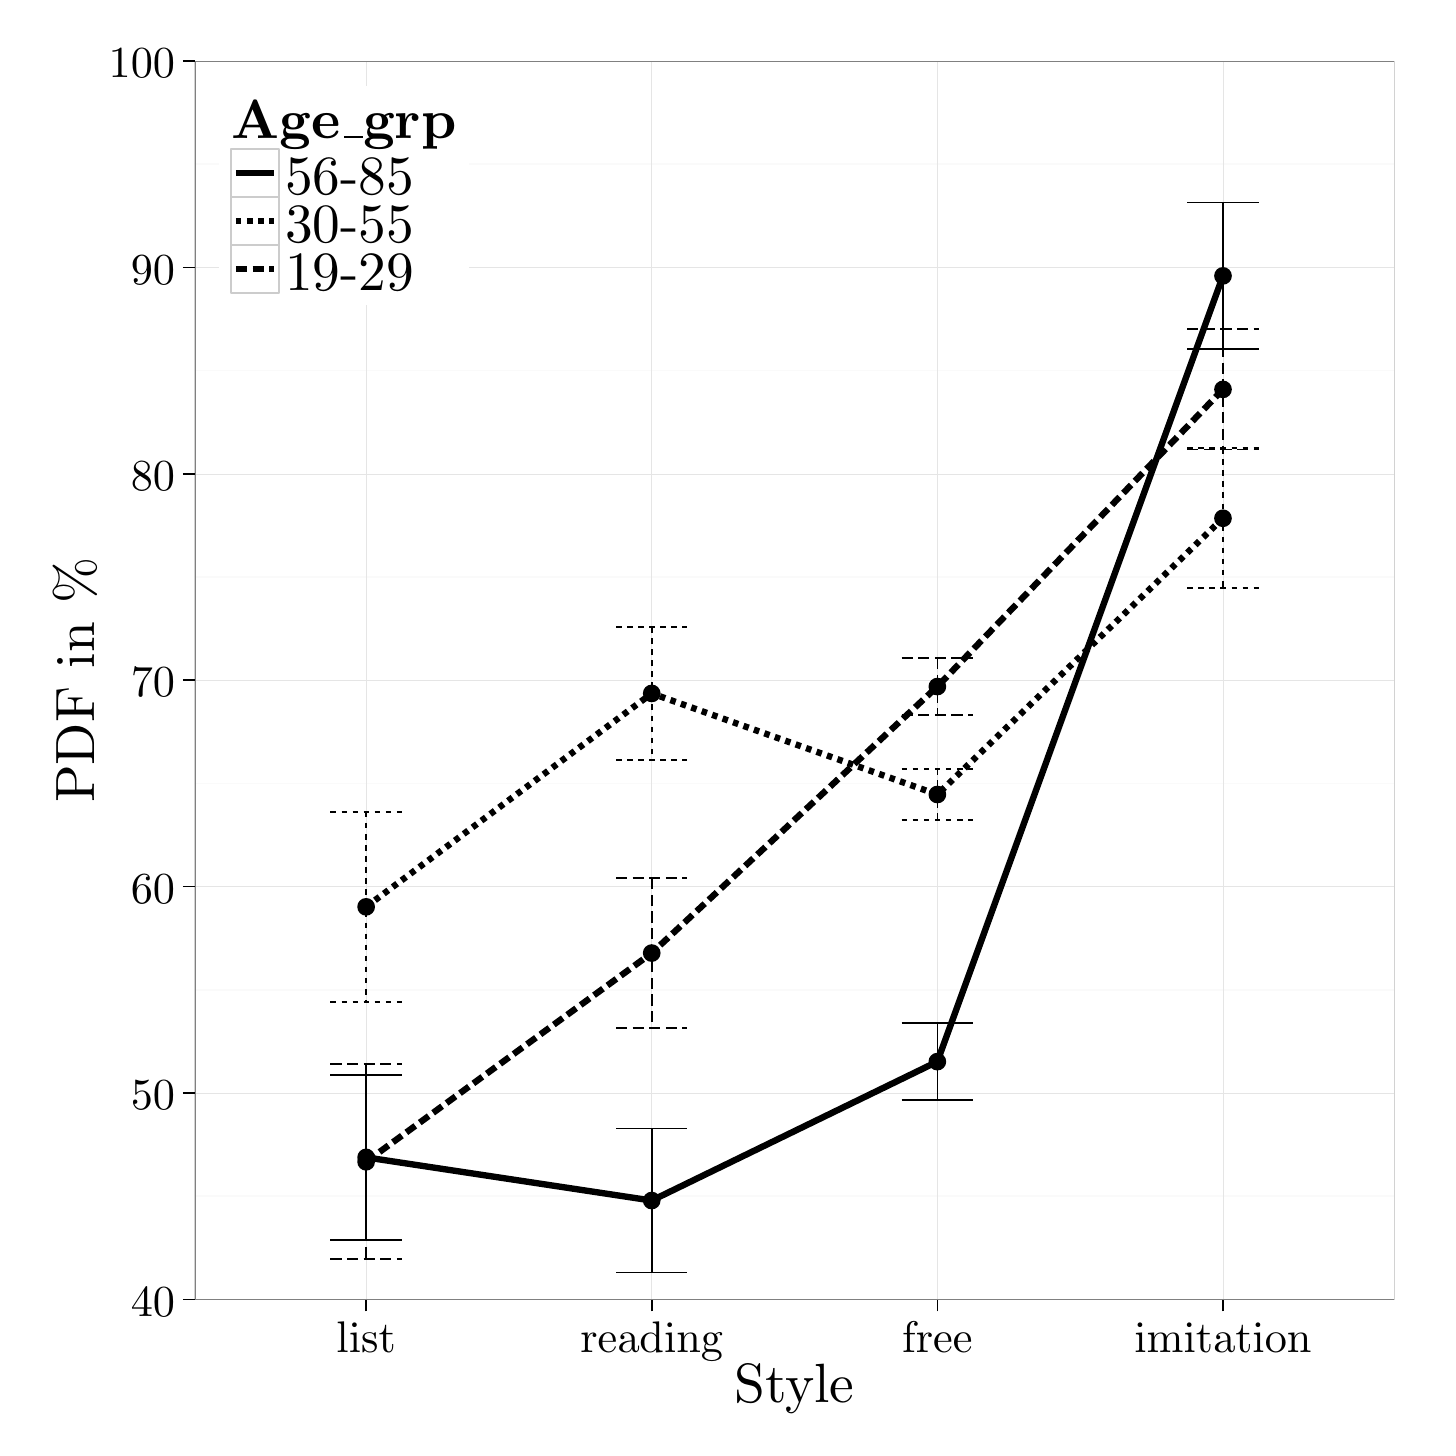
\begin{tikzpicture}[x=1pt,y=1pt]
\definecolor{fillColor}{RGB}{255,255,255}
\path[use as bounding box,fill=fillColor,fill opacity=0.00] (0,0) rectangle (505.89,505.89);
\begin{scope}
\path[clip] (  0.00,  0.00) rectangle (505.89,505.89);
\definecolor{drawColor}{RGB}{255,255,255}
\definecolor{fillColor}{RGB}{255,255,255}

\path[draw=drawColor,line width= 0.6pt,line join=round,line cap=round,fill=fillColor] (  0.00, -0.00) rectangle (505.89,505.89);
\end{scope}
\begin{scope}
\path[clip] ( 60.37, 46.31) rectangle (493.85,493.84);
\definecolor{fillColor}{RGB}{255,255,255}

\path[fill=fillColor] ( 60.37, 46.31) rectangle (493.85,493.84);
\definecolor{drawColor}{gray}{0.98}

\path[draw=drawColor,line width= 0.6pt,line join=round] ( 60.37, 83.60) --
	(493.85, 83.60);

\path[draw=drawColor,line width= 0.6pt,line join=round] ( 60.37,158.19) --
	(493.85,158.19);

\path[draw=drawColor,line width= 0.6pt,line join=round] ( 60.37,232.78) --
	(493.85,232.78);

\path[draw=drawColor,line width= 0.6pt,line join=round] ( 60.37,307.37) --
	(493.85,307.37);

\path[draw=drawColor,line width= 0.6pt,line join=round] ( 60.37,381.96) --
	(493.85,381.96);

\path[draw=drawColor,line width= 0.6pt,line join=round] ( 60.37,456.55) --
	(493.85,456.55);
\definecolor{drawColor}{gray}{0.90}

\path[draw=drawColor,line width= 0.2pt,line join=round] ( 60.37, 46.31) --
	(493.85, 46.31);

\path[draw=drawColor,line width= 0.2pt,line join=round] ( 60.37,120.90) --
	(493.85,120.90);

\path[draw=drawColor,line width= 0.2pt,line join=round] ( 60.37,195.49) --
	(493.85,195.49);

\path[draw=drawColor,line width= 0.2pt,line join=round] ( 60.37,270.08) --
	(493.85,270.08);

\path[draw=drawColor,line width= 0.2pt,line join=round] ( 60.37,344.67) --
	(493.85,344.67);

\path[draw=drawColor,line width= 0.2pt,line join=round] ( 60.37,419.26) --
	(493.85,419.26);

\path[draw=drawColor,line width= 0.2pt,line join=round] ( 60.37,493.84) --
	(493.85,493.84);

\path[draw=drawColor,line width= 0.2pt,line join=round] (122.30, 46.31) --
	(122.30,493.84);

\path[draw=drawColor,line width= 0.2pt,line join=round] (225.50, 46.31) --
	(225.50,493.84);

\path[draw=drawColor,line width= 0.2pt,line join=round] (328.71, 46.31) --
	(328.71,493.84);

\path[draw=drawColor,line width= 0.2pt,line join=round] (431.92, 46.31) --
	(431.92,493.84);
\definecolor{fillColor}{RGB}{0,0,0}

\path[fill=fillColor] (122.30, 97.67) circle (  3.20);

\path[fill=fillColor] (122.30,188.20) circle (  3.20);

\path[fill=fillColor] (122.30, 96.08) circle (  3.20);

\path[fill=fillColor] (225.50, 82.07) circle (  3.20);

\path[fill=fillColor] (225.50,265.32) circle (  3.20);

\path[fill=fillColor] (225.50,171.50) circle (  3.20);

\path[fill=fillColor] (328.71,132.27) circle (  3.20);

\path[fill=fillColor] (328.71,228.79) circle (  3.20);

\path[fill=fillColor] (328.71,267.80) circle (  3.20);

\path[fill=fillColor] (431.92,416.20) circle (  3.20);

\path[fill=fillColor] (431.92,328.61) circle (  3.20);

\path[fill=fillColor] (431.92,375.18) circle (  3.20);
\definecolor{drawColor}{RGB}{0,0,0}

\path[draw=drawColor,line width= 2.3pt,line join=round] (122.30, 97.67) --
	(225.50, 82.07) --
	(328.71,132.27) --
	(431.92,416.20);

\path[draw=drawColor,line width= 2.3pt,dash pattern=on 2pt off 2pt ,line join=round] (122.30,188.20) --
	(225.50,265.32) --
	(328.71,228.79) --
	(431.92,328.61);

\path[draw=drawColor,line width= 2.3pt,dash pattern=on 4pt off 2pt ,line join=round] (122.30, 96.08) --
	(225.50,171.50) --
	(328.71,267.80) --
	(431.92,375.18);

\path[draw=drawColor,line width= 0.6pt,line join=round] (109.40,127.53) --
	(135.20,127.53);

\path[draw=drawColor,line width= 0.6pt,line join=round] (122.30,127.53) --
	(122.30, 67.80);

\path[draw=drawColor,line width= 0.6pt,line join=round] (109.40, 67.80) --
	(135.20, 67.80);

\path[draw=drawColor,line width= 0.6pt,line join=round] (212.60,108.10) --
	(238.41,108.10);

\path[draw=drawColor,line width= 0.6pt,line join=round] (225.50,108.10) --
	(225.50, 56.04);

\path[draw=drawColor,line width= 0.6pt,line join=round] (212.60, 56.04) --
	(238.41, 56.04);

\path[draw=drawColor,line width= 0.6pt,line join=round] (315.81,146.15) --
	(341.61,146.15);

\path[draw=drawColor,line width= 0.6pt,line join=round] (328.71,146.15) --
	(328.71,118.40);

\path[draw=drawColor,line width= 0.6pt,line join=round] (315.81,118.40) --
	(341.61,118.40);

\path[draw=drawColor,line width= 0.6pt,line join=round] (419.02,442.65) --
	(444.82,442.65);

\path[draw=drawColor,line width= 0.6pt,line join=round] (431.92,442.65) --
	(431.92,389.76);

\path[draw=drawColor,line width= 0.6pt,line join=round] (419.02,389.76) --
	(444.82,389.76);

\path[draw=drawColor,line width= 0.6pt,dash pattern=on 2pt off 2pt ,line join=round] (109.40,222.51) --
	(135.20,222.51);

\path[draw=drawColor,line width= 0.6pt,dash pattern=on 2pt off 2pt ,line join=round] (122.30,222.51) --
	(122.30,153.90);

\path[draw=drawColor,line width= 0.6pt,dash pattern=on 2pt off 2pt ,line join=round] (109.40,153.90) --
	(135.20,153.90);

\path[draw=drawColor,line width= 0.6pt,dash pattern=on 2pt off 2pt ,line join=round] (212.60,289.32) --
	(238.41,289.32);

\path[draw=drawColor,line width= 0.6pt,dash pattern=on 2pt off 2pt ,line join=round] (225.50,289.32) --
	(225.50,241.32);

\path[draw=drawColor,line width= 0.6pt,dash pattern=on 2pt off 2pt ,line join=round] (212.60,241.32) --
	(238.41,241.32);

\path[draw=drawColor,line width= 0.6pt,dash pattern=on 2pt off 2pt ,line join=round] (315.81,237.95) --
	(341.61,237.95);

\path[draw=drawColor,line width= 0.6pt,dash pattern=on 2pt off 2pt ,line join=round] (328.71,237.95) --
	(328.71,219.62);

\path[draw=drawColor,line width= 0.6pt,dash pattern=on 2pt off 2pt ,line join=round] (315.81,219.62) --
	(341.61,219.62);

\path[draw=drawColor,line width= 0.6pt,dash pattern=on 2pt off 2pt ,line join=round] (419.02,353.93) --
	(444.82,353.93);

\path[draw=drawColor,line width= 0.6pt,dash pattern=on 2pt off 2pt ,line join=round] (431.92,353.93) --
	(431.92,303.30);

\path[draw=drawColor,line width= 0.6pt,dash pattern=on 2pt off 2pt ,line join=round] (419.02,303.30) --
	(444.82,303.30);

\path[draw=drawColor,line width= 0.6pt,dash pattern=on 4pt off 2pt ,line join=round] (109.40,131.30) --
	(135.20,131.30);

\path[draw=drawColor,line width= 0.6pt,dash pattern=on 4pt off 2pt ,line join=round] (122.30,131.30) --
	(122.30, 60.85);

\path[draw=drawColor,line width= 0.6pt,dash pattern=on 4pt off 2pt ,line join=round] (109.40, 60.85) --
	(135.20, 60.85);

\path[draw=drawColor,line width= 0.6pt,dash pattern=on 4pt off 2pt ,line join=round] (212.60,198.53) --
	(238.41,198.53);

\path[draw=drawColor,line width= 0.6pt,dash pattern=on 4pt off 2pt ,line join=round] (225.50,198.53) --
	(225.50,144.47);

\path[draw=drawColor,line width= 0.6pt,dash pattern=on 4pt off 2pt ,line join=round] (212.60,144.47) --
	(238.41,144.47);

\path[draw=drawColor,line width= 0.6pt,dash pattern=on 4pt off 2pt ,line join=round] (315.81,278.02) --
	(341.61,278.02);

\path[draw=drawColor,line width= 0.6pt,dash pattern=on 4pt off 2pt ,line join=round] (328.71,278.02) --
	(328.71,257.58);

\path[draw=drawColor,line width= 0.6pt,dash pattern=on 4pt off 2pt ,line join=round] (315.81,257.58) --
	(341.61,257.58);

\path[draw=drawColor,line width= 0.6pt,dash pattern=on 4pt off 2pt ,line join=round] (419.02,396.89) --
	(444.82,396.89);

\path[draw=drawColor,line width= 0.6pt,dash pattern=on 4pt off 2pt ,line join=round] (431.92,396.89) --
	(431.92,353.48);

\path[draw=drawColor,line width= 0.6pt,dash pattern=on 4pt off 2pt ,line join=round] (419.02,353.48) --
	(444.82,353.48);
\definecolor{drawColor}{gray}{0.50}

\path[draw=drawColor,line width= 0.6pt,line join=round,line cap=round] ( 60.37, 46.31) rectangle (493.85,493.84);
\end{scope}
\begin{scope}
\path[clip] (  0.00,  0.00) rectangle (505.89,505.89);
\definecolor{drawColor}{RGB}{0,0,0}

\node[text=drawColor,anchor=base east,inner sep=0pt, outer sep=0pt, scale=  1.60] at ( 53.26, 40.27) {40};

\node[text=drawColor,anchor=base east,inner sep=0pt, outer sep=0pt, scale=  1.60] at ( 53.26,114.86) {50};

\node[text=drawColor,anchor=base east,inner sep=0pt, outer sep=0pt, scale=  1.60] at ( 53.26,189.45) {60};

\node[text=drawColor,anchor=base east,inner sep=0pt, outer sep=0pt, scale=  1.60] at ( 53.26,264.04) {70};

\node[text=drawColor,anchor=base east,inner sep=0pt, outer sep=0pt, scale=  1.60] at ( 53.26,338.63) {80};

\node[text=drawColor,anchor=base east,inner sep=0pt, outer sep=0pt, scale=  1.60] at ( 53.26,413.22) {90};

\node[text=drawColor,anchor=base east,inner sep=0pt, outer sep=0pt, scale=  1.60] at ( 53.26,487.81) {100};
\end{scope}
\begin{scope}
\path[clip] (  0.00,  0.00) rectangle (505.89,505.89);
\definecolor{drawColor}{RGB}{0,0,0}

\path[draw=drawColor,line width= 0.6pt,line join=round] ( 56.10, 46.31) --
	( 60.37, 46.31);

\path[draw=drawColor,line width= 0.6pt,line join=round] ( 56.10,120.90) --
	( 60.37,120.90);

\path[draw=drawColor,line width= 0.6pt,line join=round] ( 56.10,195.49) --
	( 60.37,195.49);

\path[draw=drawColor,line width= 0.6pt,line join=round] ( 56.10,270.08) --
	( 60.37,270.08);

\path[draw=drawColor,line width= 0.6pt,line join=round] ( 56.10,344.67) --
	( 60.37,344.67);

\path[draw=drawColor,line width= 0.6pt,line join=round] ( 56.10,419.26) --
	( 60.37,419.26);

\path[draw=drawColor,line width= 0.6pt,line join=round] ( 56.10,493.84) --
	( 60.37,493.84);
\end{scope}
\begin{scope}
\path[clip] (  0.00,  0.00) rectangle (505.89,505.89);
\definecolor{drawColor}{RGB}{0,0,0}

\path[draw=drawColor,line width= 0.6pt,line join=round] (122.30, 42.04) --
	(122.30, 46.31);

\path[draw=drawColor,line width= 0.6pt,line join=round] (225.50, 42.04) --
	(225.50, 46.31);

\path[draw=drawColor,line width= 0.6pt,line join=round] (328.71, 42.04) --
	(328.71, 46.31);

\path[draw=drawColor,line width= 0.6pt,line join=round] (431.92, 42.04) --
	(431.92, 46.31);
\end{scope}
\begin{scope}
\path[clip] (  0.00,  0.00) rectangle (505.89,505.89);
\definecolor{drawColor}{RGB}{0,0,0}

\node[text=drawColor,anchor=base,inner sep=0pt, outer sep=0pt, scale=  1.60] at (122.30, 27.13) {list};

\node[text=drawColor,anchor=base,inner sep=0pt, outer sep=0pt, scale=  1.60] at (225.50, 27.13) {reading};

\node[text=drawColor,anchor=base,inner sep=0pt, outer sep=0pt, scale=  1.60] at (328.71, 27.13) {free};

\node[text=drawColor,anchor=base,inner sep=0pt, outer sep=0pt, scale=  1.60] at (431.92, 27.13) {imitation};
\end{scope}
\begin{scope}
\path[clip] (  0.00,  0.00) rectangle (505.89,505.89);
\definecolor{drawColor}{RGB}{0,0,0}

\node[text=drawColor,anchor=base,inner sep=0pt, outer sep=0pt, scale=  2.00] at (277.11,  9.03) {Style};
\end{scope}
\begin{scope}
\path[clip] (  0.00,  0.00) rectangle (505.89,505.89);
\definecolor{drawColor}{RGB}{0,0,0}

\node[text=drawColor,rotate= 90.00,anchor=base,inner sep=0pt, outer sep=0pt, scale=  2.00] at ( 24.12,270.08) {PDF in {\%}};
\end{scope}
\begin{scope}
\path[clip] (  0.00,  0.00) rectangle (505.89,505.89);
\definecolor{fillColor}{RGB}{255,255,255}

\path[fill=fillColor] ( 69.24,405.66) rectangle (159.40,484.98);
\end{scope}
\begin{scope}
\path[clip] (  0.00,  0.00) rectangle (505.89,505.89);
\definecolor{drawColor}{RGB}{0,0,0}

\node[text=drawColor,anchor=base west,inner sep=0pt, outer sep=0pt, scale=  2.00] at ( 73.51,465.96) {\bfseries Age{\_{}}grp};
\end{scope}
\begin{scope}
\path[clip] (  0.00,  0.00) rectangle (505.89,505.89);
\definecolor{drawColor}{gray}{0.80}
\definecolor{fillColor}{RGB}{255,255,255}

\path[draw=drawColor,line width= 0.6pt,line join=round,line cap=round,fill=fillColor] ( 73.51,444.61) rectangle ( 90.85,461.96);
\end{scope}
\begin{scope}
\path[clip] (  0.00,  0.00) rectangle (505.89,505.89);
\definecolor{drawColor}{RGB}{0,0,0}

\path[draw=drawColor,line width= 2.3pt,line join=round] ( 75.24,453.29) -- ( 89.12,453.29);
\end{scope}
\begin{scope}
\path[clip] (  0.00,  0.00) rectangle (505.89,505.89);
\definecolor{drawColor}{RGB}{0,0,0}

\path[draw=drawColor,line width= 0.6pt,line join=round] ( 75.24,453.29) -- ( 89.12,453.29);
\end{scope}
\begin{scope}
\path[clip] (  0.00,  0.00) rectangle (505.89,505.89);
\definecolor{drawColor}{gray}{0.80}
\definecolor{fillColor}{RGB}{255,255,255}

\path[draw=drawColor,line width= 0.6pt,line join=round,line cap=round,fill=fillColor] ( 73.51,427.27) rectangle ( 90.85,444.61);
\end{scope}
\begin{scope}
\path[clip] (  0.00,  0.00) rectangle (505.89,505.89);
\definecolor{drawColor}{RGB}{0,0,0}

\path[draw=drawColor,line width= 2.3pt,dash pattern=on 2pt off 2pt ,line join=round] ( 75.24,435.94) -- ( 89.12,435.94);
\end{scope}
\begin{scope}
\path[clip] (  0.00,  0.00) rectangle (505.89,505.89);
\definecolor{drawColor}{RGB}{0,0,0}

\path[draw=drawColor,line width= 0.6pt,dash pattern=on 2pt off 2pt ,line join=round] ( 75.24,435.94) -- ( 89.12,435.94);
\end{scope}
\begin{scope}
\path[clip] (  0.00,  0.00) rectangle (505.89,505.89);
\definecolor{drawColor}{gray}{0.80}
\definecolor{fillColor}{RGB}{255,255,255}

\path[draw=drawColor,line width= 0.6pt,line join=round,line cap=round,fill=fillColor] ( 73.51,409.92) rectangle ( 90.85,427.27);
\end{scope}
\begin{scope}
\path[clip] (  0.00,  0.00) rectangle (505.89,505.89);
\definecolor{drawColor}{RGB}{0,0,0}

\path[draw=drawColor,line width= 2.3pt,dash pattern=on 4pt off 2pt ,line join=round] ( 75.24,418.60) -- ( 89.12,418.60);
\end{scope}
\begin{scope}
\path[clip] (  0.00,  0.00) rectangle (505.89,505.89);
\definecolor{drawColor}{RGB}{0,0,0}

\path[draw=drawColor,line width= 0.6pt,dash pattern=on 4pt off 2pt ,line join=round] ( 75.24,418.60) -- ( 89.12,418.60);
\end{scope}
\begin{scope}
\path[clip] (  0.00,  0.00) rectangle (505.89,505.89);
\definecolor{drawColor}{RGB}{0,0,0}

\node[text=drawColor,anchor=base west,inner sep=0pt, outer sep=0pt, scale=  2.00] at ( 93.02,445.75) {56-85};
\end{scope}
\begin{scope}
\path[clip] (  0.00,  0.00) rectangle (505.89,505.89);
\definecolor{drawColor}{RGB}{0,0,0}

\node[text=drawColor,anchor=base west,inner sep=0pt, outer sep=0pt, scale=  2.00] at ( 93.02,428.40) {30-55};
\end{scope}
\begin{scope}
\path[clip] (  0.00,  0.00) rectangle (505.89,505.89);
\definecolor{drawColor}{RGB}{0,0,0}

\node[text=drawColor,anchor=base west,inner sep=0pt, outer sep=0pt, scale=  2.00] at ( 93.02,411.06) {19-29};
\end{scope}
\end{tikzpicture}
} 
		\caption{women}
		\label{fig.line.k.fem}
	\end{subfigure}
	\begin{subfigure}{.49\textwidth}
		\centering
			\definecolor{shadecolor}{rgb}{0.969, 0.969, 0.969}
			\resizebox{\linewidth}{!}{% Created by tikzDevice version 0.8.1 on 2016-02-09 02:17:39
% !TEX encoding = UTF-8 Unicode
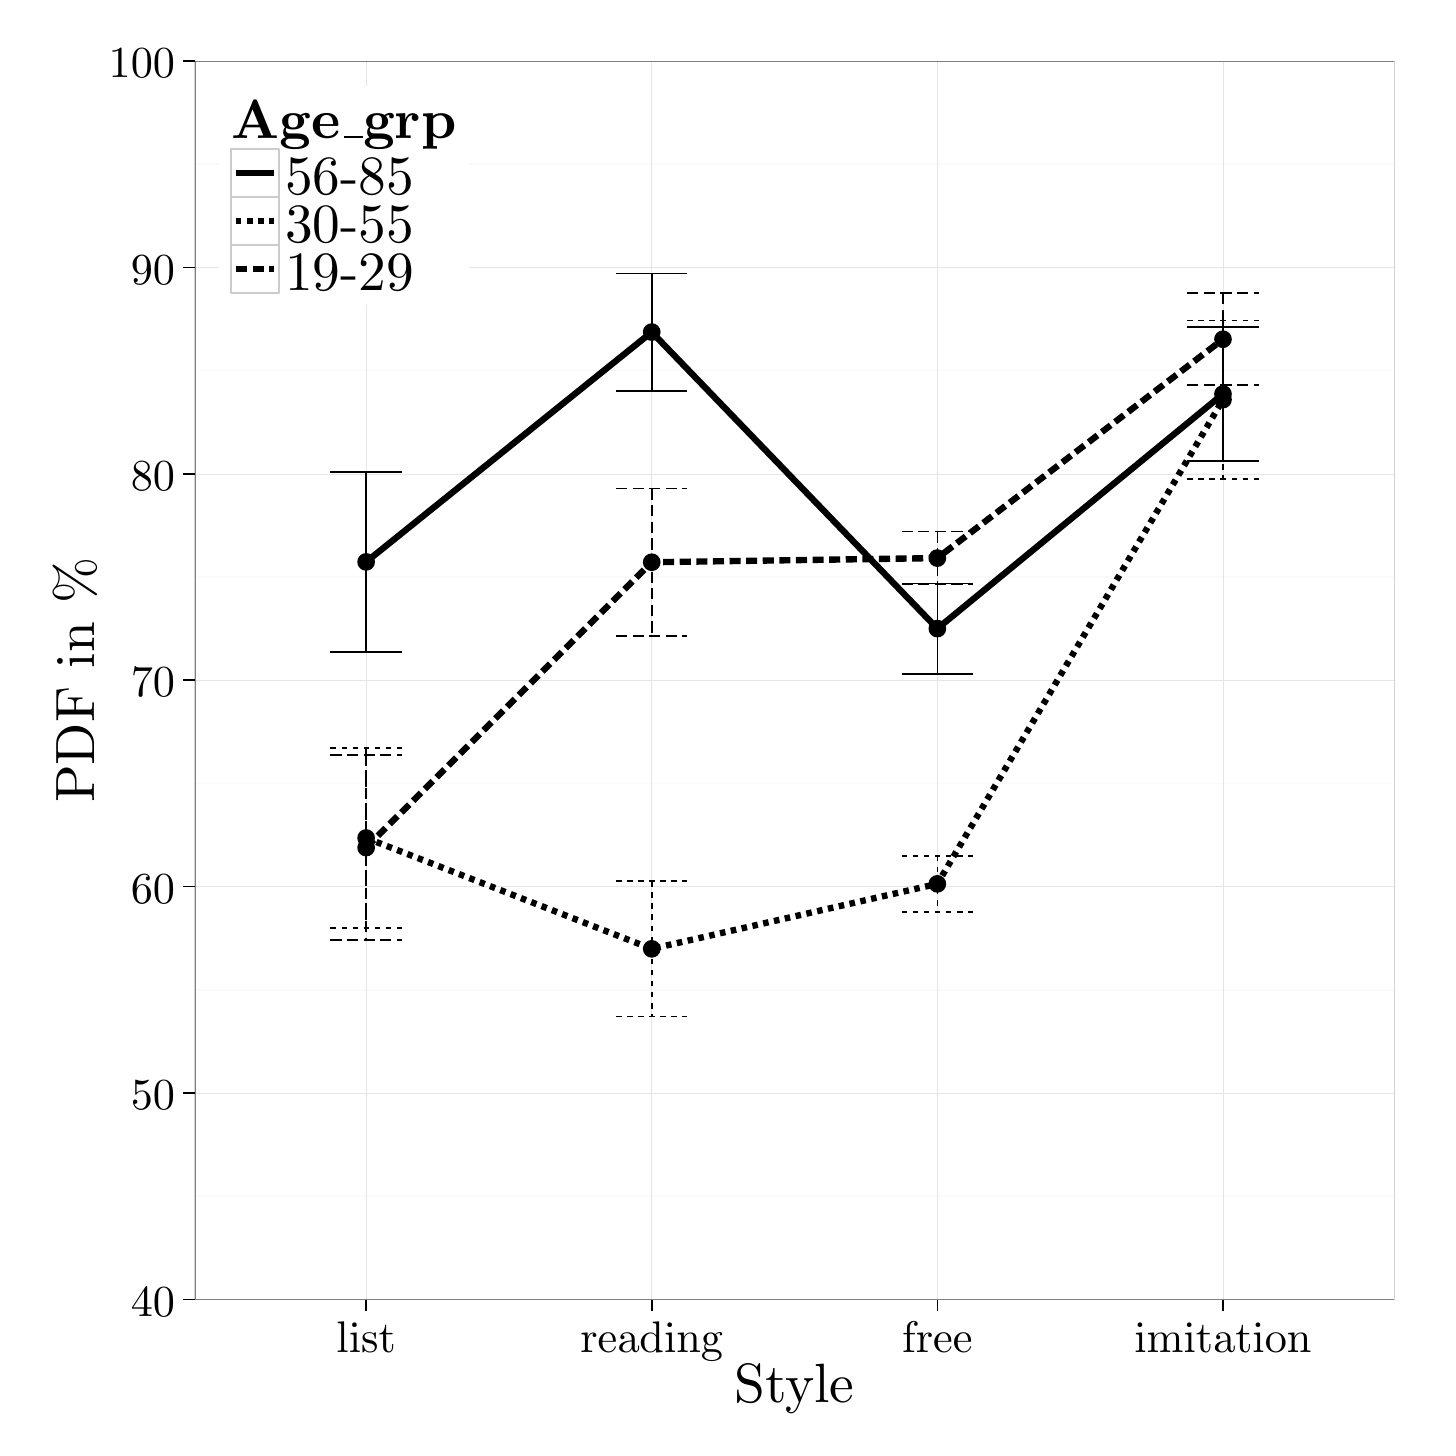
\begin{tikzpicture}[x=1pt,y=1pt]
\definecolor{fillColor}{RGB}{255,255,255}
\path[use as bounding box,fill=fillColor,fill opacity=0.00] (0,0) rectangle (505.89,505.89);
\begin{scope}
\path[clip] (  0.00,  0.00) rectangle (505.89,505.89);
\definecolor{drawColor}{RGB}{255,255,255}
\definecolor{fillColor}{RGB}{255,255,255}

\path[draw=drawColor,line width= 0.6pt,line join=round,line cap=round,fill=fillColor] (  0.00, -0.00) rectangle (505.89,505.89);
\end{scope}
\begin{scope}
\path[clip] ( 60.37, 46.31) rectangle (493.85,493.84);
\definecolor{fillColor}{RGB}{255,255,255}

\path[fill=fillColor] ( 60.37, 46.31) rectangle (493.85,493.84);
\definecolor{drawColor}{gray}{0.98}

\path[draw=drawColor,line width= 0.6pt,line join=round] ( 60.37, 83.60) --
	(493.85, 83.60);

\path[draw=drawColor,line width= 0.6pt,line join=round] ( 60.37,158.19) --
	(493.85,158.19);

\path[draw=drawColor,line width= 0.6pt,line join=round] ( 60.37,232.78) --
	(493.85,232.78);

\path[draw=drawColor,line width= 0.6pt,line join=round] ( 60.37,307.37) --
	(493.85,307.37);

\path[draw=drawColor,line width= 0.6pt,line join=round] ( 60.37,381.96) --
	(493.85,381.96);

\path[draw=drawColor,line width= 0.6pt,line join=round] ( 60.37,456.55) --
	(493.85,456.55);
\definecolor{drawColor}{gray}{0.90}

\path[draw=drawColor,line width= 0.2pt,line join=round] ( 60.37, 46.31) --
	(493.85, 46.31);

\path[draw=drawColor,line width= 0.2pt,line join=round] ( 60.37,120.90) --
	(493.85,120.90);

\path[draw=drawColor,line width= 0.2pt,line join=round] ( 60.37,195.49) --
	(493.85,195.49);

\path[draw=drawColor,line width= 0.2pt,line join=round] ( 60.37,270.08) --
	(493.85,270.08);

\path[draw=drawColor,line width= 0.2pt,line join=round] ( 60.37,344.67) --
	(493.85,344.67);

\path[draw=drawColor,line width= 0.2pt,line join=round] ( 60.37,419.26) --
	(493.85,419.26);

\path[draw=drawColor,line width= 0.2pt,line join=round] ( 60.37,493.84) --
	(493.85,493.84);

\path[draw=drawColor,line width= 0.2pt,line join=round] (122.30, 46.31) --
	(122.30,493.84);

\path[draw=drawColor,line width= 0.2pt,line join=round] (225.50, 46.31) --
	(225.50,493.84);

\path[draw=drawColor,line width= 0.2pt,line join=round] (328.71, 46.31) --
	(328.71,493.84);

\path[draw=drawColor,line width= 0.2pt,line join=round] (431.92, 46.31) --
	(431.92,493.84);
\definecolor{fillColor}{RGB}{0,0,0}

\path[fill=fillColor] (122.30,312.84) circle (  3.20);

\path[fill=fillColor] (122.30,213.08) circle (  3.20);

\path[fill=fillColor] (122.30,209.61) circle (  3.20);

\path[fill=fillColor] (225.50,395.89) circle (  3.20);

\path[fill=fillColor] (225.50,173.02) circle (  3.20);

\path[fill=fillColor] (225.50,312.72) circle (  3.20);

\path[fill=fillColor] (328.71,288.74) circle (  3.20);

\path[fill=fillColor] (328.71,196.50) circle (  3.20);

\path[fill=fillColor] (328.71,314.22) circle (  3.20);

\path[fill=fillColor] (431.92,373.52) circle (  3.20);

\path[fill=fillColor] (431.92,371.48) circle (  3.20);

\path[fill=fillColor] (431.92,393.31) circle (  3.20);
\definecolor{drawColor}{RGB}{0,0,0}

\path[draw=drawColor,line width= 2.3pt,line join=round] (122.30,312.84) --
	(225.50,395.89) --
	(328.71,288.74) --
	(431.92,373.52);

\path[draw=drawColor,line width= 2.3pt,dash pattern=on 2pt off 2pt ,line join=round] (122.30,213.08) --
	(225.50,173.02) --
	(328.71,196.50) --
	(431.92,371.48);

\path[draw=drawColor,line width= 2.3pt,dash pattern=on 4pt off 2pt ,line join=round] (122.30,209.61) --
	(225.50,312.72) --
	(328.71,314.22) --
	(431.92,393.31);

\path[draw=drawColor,line width= 0.6pt,line join=round] (109.40,345.38) --
	(135.20,345.38);

\path[draw=drawColor,line width= 0.6pt,line join=round] (122.30,345.38) --
	(122.30,280.30);

\path[draw=drawColor,line width= 0.6pt,line join=round] (109.40,280.30) --
	(135.20,280.30);

\path[draw=drawColor,line width= 0.6pt,line join=round] (212.60,417.08) --
	(238.41,417.08);

\path[draw=drawColor,line width= 0.6pt,line join=round] (225.50,417.08) --
	(225.50,374.69);

\path[draw=drawColor,line width= 0.6pt,line join=round] (212.60,374.69) --
	(238.41,374.69);

\path[draw=drawColor,line width= 0.6pt,line join=round] (315.81,305.05) --
	(341.61,305.05);

\path[draw=drawColor,line width= 0.6pt,line join=round] (328.71,305.05) --
	(328.71,272.42);

\path[draw=drawColor,line width= 0.6pt,line join=round] (315.81,272.42) --
	(341.61,272.42);

\path[draw=drawColor,line width= 0.6pt,line join=round] (419.02,397.61) --
	(444.82,397.61);

\path[draw=drawColor,line width= 0.6pt,line join=round] (431.92,397.61) --
	(431.92,349.42);

\path[draw=drawColor,line width= 0.6pt,line join=round] (419.02,349.42) --
	(444.82,349.42);

\path[draw=drawColor,line width= 0.6pt,dash pattern=on 2pt off 2pt ,line join=round] (109.40,245.55) --
	(135.20,245.55);

\path[draw=drawColor,line width= 0.6pt,dash pattern=on 2pt off 2pt ,line join=round] (122.30,245.55) --
	(122.30,180.62);

\path[draw=drawColor,line width= 0.6pt,dash pattern=on 2pt off 2pt ,line join=round] (109.40,180.62) --
	(135.20,180.62);

\path[draw=drawColor,line width= 0.6pt,dash pattern=on 2pt off 2pt ,line join=round] (212.60,197.45) --
	(238.41,197.45);

\path[draw=drawColor,line width= 0.6pt,dash pattern=on 2pt off 2pt ,line join=round] (225.50,197.45) --
	(225.50,148.58);

\path[draw=drawColor,line width= 0.6pt,dash pattern=on 2pt off 2pt ,line join=round] (212.60,148.58) --
	(238.41,148.58);

\path[draw=drawColor,line width= 0.6pt,dash pattern=on 2pt off 2pt ,line join=round] (315.81,206.66) --
	(341.61,206.66);

\path[draw=drawColor,line width= 0.6pt,dash pattern=on 2pt off 2pt ,line join=round] (328.71,206.66) --
	(328.71,186.33);

\path[draw=drawColor,line width= 0.6pt,dash pattern=on 2pt off 2pt ,line join=round] (315.81,186.33) --
	(341.61,186.33);

\path[draw=drawColor,line width= 0.6pt,dash pattern=on 2pt off 2pt ,line join=round] (419.02,400.11) --
	(444.82,400.11);

\path[draw=drawColor,line width= 0.6pt,dash pattern=on 2pt off 2pt ,line join=round] (431.92,400.11) --
	(431.92,342.84);

\path[draw=drawColor,line width= 0.6pt,dash pattern=on 2pt off 2pt ,line join=round] (419.02,342.84) --
	(444.82,342.84);

\path[draw=drawColor,line width= 0.6pt,dash pattern=on 4pt off 2pt ,line join=round] (109.40,243.10) --
	(135.20,243.10);

\path[draw=drawColor,line width= 0.6pt,dash pattern=on 4pt off 2pt ,line join=round] (122.30,243.10) --
	(122.30,176.12);

\path[draw=drawColor,line width= 0.6pt,dash pattern=on 4pt off 2pt ,line join=round] (109.40,176.12) --
	(135.20,176.12);

\path[draw=drawColor,line width= 0.6pt,dash pattern=on 4pt off 2pt ,line join=round] (212.60,339.32) --
	(238.41,339.32);

\path[draw=drawColor,line width= 0.6pt,dash pattern=on 4pt off 2pt ,line join=round] (225.50,339.32) --
	(225.50,286.13);

\path[draw=drawColor,line width= 0.6pt,dash pattern=on 4pt off 2pt ,line join=round] (212.60,286.13) --
	(238.41,286.13);

\path[draw=drawColor,line width= 0.6pt,dash pattern=on 4pt off 2pt ,line join=round] (315.81,323.80) --
	(341.61,323.80);

\path[draw=drawColor,line width= 0.6pt,dash pattern=on 4pt off 2pt ,line join=round] (328.71,323.80) --
	(328.71,304.63);

\path[draw=drawColor,line width= 0.6pt,dash pattern=on 4pt off 2pt ,line join=round] (315.81,304.63) --
	(341.61,304.63);

\path[draw=drawColor,line width= 0.6pt,dash pattern=on 4pt off 2pt ,line join=round] (419.02,409.92) --
	(444.82,409.92);

\path[draw=drawColor,line width= 0.6pt,dash pattern=on 4pt off 2pt ,line join=round] (431.92,409.92) --
	(431.92,376.70);

\path[draw=drawColor,line width= 0.6pt,dash pattern=on 4pt off 2pt ,line join=round] (419.02,376.70) --
	(444.82,376.70);
\definecolor{drawColor}{gray}{0.50}

\path[draw=drawColor,line width= 0.6pt,line join=round,line cap=round] ( 60.37, 46.31) rectangle (493.85,493.84);
\end{scope}
\begin{scope}
\path[clip] (  0.00,  0.00) rectangle (505.89,505.89);
\definecolor{drawColor}{RGB}{0,0,0}

\node[text=drawColor,anchor=base east,inner sep=0pt, outer sep=0pt, scale=  1.60] at ( 53.26, 40.27) {40};

\node[text=drawColor,anchor=base east,inner sep=0pt, outer sep=0pt, scale=  1.60] at ( 53.26,114.86) {50};

\node[text=drawColor,anchor=base east,inner sep=0pt, outer sep=0pt, scale=  1.60] at ( 53.26,189.45) {60};

\node[text=drawColor,anchor=base east,inner sep=0pt, outer sep=0pt, scale=  1.60] at ( 53.26,264.04) {70};

\node[text=drawColor,anchor=base east,inner sep=0pt, outer sep=0pt, scale=  1.60] at ( 53.26,338.63) {80};

\node[text=drawColor,anchor=base east,inner sep=0pt, outer sep=0pt, scale=  1.60] at ( 53.26,413.22) {90};

\node[text=drawColor,anchor=base east,inner sep=0pt, outer sep=0pt, scale=  1.60] at ( 53.26,487.81) {100};
\end{scope}
\begin{scope}
\path[clip] (  0.00,  0.00) rectangle (505.89,505.89);
\definecolor{drawColor}{RGB}{0,0,0}

\path[draw=drawColor,line width= 0.6pt,line join=round] ( 56.10, 46.31) --
	( 60.37, 46.31);

\path[draw=drawColor,line width= 0.6pt,line join=round] ( 56.10,120.90) --
	( 60.37,120.90);

\path[draw=drawColor,line width= 0.6pt,line join=round] ( 56.10,195.49) --
	( 60.37,195.49);

\path[draw=drawColor,line width= 0.6pt,line join=round] ( 56.10,270.08) --
	( 60.37,270.08);

\path[draw=drawColor,line width= 0.6pt,line join=round] ( 56.10,344.67) --
	( 60.37,344.67);

\path[draw=drawColor,line width= 0.6pt,line join=round] ( 56.10,419.26) --
	( 60.37,419.26);

\path[draw=drawColor,line width= 0.6pt,line join=round] ( 56.10,493.84) --
	( 60.37,493.84);
\end{scope}
\begin{scope}
\path[clip] (  0.00,  0.00) rectangle (505.89,505.89);
\definecolor{drawColor}{RGB}{0,0,0}

\path[draw=drawColor,line width= 0.6pt,line join=round] (122.30, 42.04) --
	(122.30, 46.31);

\path[draw=drawColor,line width= 0.6pt,line join=round] (225.50, 42.04) --
	(225.50, 46.31);

\path[draw=drawColor,line width= 0.6pt,line join=round] (328.71, 42.04) --
	(328.71, 46.31);

\path[draw=drawColor,line width= 0.6pt,line join=round] (431.92, 42.04) --
	(431.92, 46.31);
\end{scope}
\begin{scope}
\path[clip] (  0.00,  0.00) rectangle (505.89,505.89);
\definecolor{drawColor}{RGB}{0,0,0}

\node[text=drawColor,anchor=base,inner sep=0pt, outer sep=0pt, scale=  1.60] at (122.30, 27.13) {list};

\node[text=drawColor,anchor=base,inner sep=0pt, outer sep=0pt, scale=  1.60] at (225.50, 27.13) {reading};

\node[text=drawColor,anchor=base,inner sep=0pt, outer sep=0pt, scale=  1.60] at (328.71, 27.13) {free};

\node[text=drawColor,anchor=base,inner sep=0pt, outer sep=0pt, scale=  1.60] at (431.92, 27.13) {imitation};
\end{scope}
\begin{scope}
\path[clip] (  0.00,  0.00) rectangle (505.89,505.89);
\definecolor{drawColor}{RGB}{0,0,0}

\node[text=drawColor,anchor=base,inner sep=0pt, outer sep=0pt, scale=  2.00] at (277.11,  9.03) {Style};
\end{scope}
\begin{scope}
\path[clip] (  0.00,  0.00) rectangle (505.89,505.89);
\definecolor{drawColor}{RGB}{0,0,0}

\node[text=drawColor,rotate= 90.00,anchor=base,inner sep=0pt, outer sep=0pt, scale=  2.00] at ( 24.12,270.08) {PDF in {\%}};
\end{scope}
\begin{scope}
\path[clip] (  0.00,  0.00) rectangle (505.89,505.89);
\definecolor{fillColor}{RGB}{255,255,255}

\path[fill=fillColor] ( 69.24,405.66) rectangle (159.40,484.98);
\end{scope}
\begin{scope}
\path[clip] (  0.00,  0.00) rectangle (505.89,505.89);
\definecolor{drawColor}{RGB}{0,0,0}

\node[text=drawColor,anchor=base west,inner sep=0pt, outer sep=0pt, scale=  2.00] at ( 73.51,465.96) {\bfseries Age{\_{}}grp};
\end{scope}
\begin{scope}
\path[clip] (  0.00,  0.00) rectangle (505.89,505.89);
\definecolor{drawColor}{gray}{0.80}
\definecolor{fillColor}{RGB}{255,255,255}

\path[draw=drawColor,line width= 0.6pt,line join=round,line cap=round,fill=fillColor] ( 73.51,444.61) rectangle ( 90.85,461.96);
\end{scope}
\begin{scope}
\path[clip] (  0.00,  0.00) rectangle (505.89,505.89);
\definecolor{drawColor}{RGB}{0,0,0}

\path[draw=drawColor,line width= 2.3pt,line join=round] ( 75.24,453.29) -- ( 89.12,453.29);
\end{scope}
\begin{scope}
\path[clip] (  0.00,  0.00) rectangle (505.89,505.89);
\definecolor{drawColor}{RGB}{0,0,0}

\path[draw=drawColor,line width= 0.6pt,line join=round] ( 75.24,453.29) -- ( 89.12,453.29);
\end{scope}
\begin{scope}
\path[clip] (  0.00,  0.00) rectangle (505.89,505.89);
\definecolor{drawColor}{gray}{0.80}
\definecolor{fillColor}{RGB}{255,255,255}

\path[draw=drawColor,line width= 0.6pt,line join=round,line cap=round,fill=fillColor] ( 73.51,427.27) rectangle ( 90.85,444.61);
\end{scope}
\begin{scope}
\path[clip] (  0.00,  0.00) rectangle (505.89,505.89);
\definecolor{drawColor}{RGB}{0,0,0}

\path[draw=drawColor,line width= 2.3pt,dash pattern=on 2pt off 2pt ,line join=round] ( 75.24,435.94) -- ( 89.12,435.94);
\end{scope}
\begin{scope}
\path[clip] (  0.00,  0.00) rectangle (505.89,505.89);
\definecolor{drawColor}{RGB}{0,0,0}

\path[draw=drawColor,line width= 0.6pt,dash pattern=on 2pt off 2pt ,line join=round] ( 75.24,435.94) -- ( 89.12,435.94);
\end{scope}
\begin{scope}
\path[clip] (  0.00,  0.00) rectangle (505.89,505.89);
\definecolor{drawColor}{gray}{0.80}
\definecolor{fillColor}{RGB}{255,255,255}

\path[draw=drawColor,line width= 0.6pt,line join=round,line cap=round,fill=fillColor] ( 73.51,409.92) rectangle ( 90.85,427.27);
\end{scope}
\begin{scope}
\path[clip] (  0.00,  0.00) rectangle (505.89,505.89);
\definecolor{drawColor}{RGB}{0,0,0}

\path[draw=drawColor,line width= 2.3pt,dash pattern=on 4pt off 2pt ,line join=round] ( 75.24,418.60) -- ( 89.12,418.60);
\end{scope}
\begin{scope}
\path[clip] (  0.00,  0.00) rectangle (505.89,505.89);
\definecolor{drawColor}{RGB}{0,0,0}

\path[draw=drawColor,line width= 0.6pt,dash pattern=on 4pt off 2pt ,line join=round] ( 75.24,418.60) -- ( 89.12,418.60);
\end{scope}
\begin{scope}
\path[clip] (  0.00,  0.00) rectangle (505.89,505.89);
\definecolor{drawColor}{RGB}{0,0,0}

\node[text=drawColor,anchor=base west,inner sep=0pt, outer sep=0pt, scale=  2.00] at ( 93.02,445.75) {56-85};
\end{scope}
\begin{scope}
\path[clip] (  0.00,  0.00) rectangle (505.89,505.89);
\definecolor{drawColor}{RGB}{0,0,0}

\node[text=drawColor,anchor=base west,inner sep=0pt, outer sep=0pt, scale=  2.00] at ( 93.02,428.40) {30-55};
\end{scope}
\begin{scope}
\path[clip] (  0.00,  0.00) rectangle (505.89,505.89);
\definecolor{drawColor}{RGB}{0,0,0}

\node[text=drawColor,anchor=base west,inner sep=0pt, outer sep=0pt, scale=  2.00] at ( 93.02,411.06) {19-29};
\end{scope}
\end{tikzpicture}
} 
		\caption{men}
		\label{fig.line.k.mal}
	\end{subfigure}
	\caption{/k/: PDF by style, age group, and gender (released only)}
\end{figure}

Since the mixed linear effects regression model found significant three-way interactions of style and age group with gender and social class, respectively, we will look at both of these as well before closing this section.
\figref{fig.line.k.fem} and \figref{fig.line.k.mal} visualise the style X age interaction for women and men separately.
If we focus on the old speakers, women show much more systematic \isi{style shifting} than men.
Provided we ignore the word list, there is actually a near linear (and significant) rise from the text passage to spontaneous speech to accent perform\is{accent performance}ance.
This rather clear picture is only spoilt by the fact that the word list is not significantly different from the reading passage, or from observations made during spontaneous speech (although in the latter case the difference is close to significance, error whiskers only just overlap).
Old men, on the other hand, show a zigzag pattern, which does not look at all like Labovian \isi{style shifting}.
Mean \isi{PDF} is high in all registers, but there are still significant differences between the two blocks `list'/`free' and `reading'/`imitation\is{accent performance}': /k/ realisations are even more lenited in the latter case than in the former.

In the middle aged group (dotted line) differences are smaller.
Women exhibit a trend towards the typical \isi{style shifting} pattern (increasing \isi{PDF} from left to right), although some curious results were obtained for the registers `reading' and `free' -- women actually use (slightly, but significantly) more Scouse realisations in the more formal text reading task than in spontaneous speech.
Men, on the other hand, have the same mean \isi{PDF}, statistically speaking, in the three `natural' styles word list, reading passage, and free speech.
This is followed by a steep rise into accent perform\is{accent performance}ance on the right-hand side of the graph, which is similar to the one found for women of this age group.
All in all, the pattern found for middle-aged men looks very much like the one revealed in \figref{fig.line.k.tot} for the entire age group.

For the youngest speakers (dashed) we find systematic \isi{style shifting} in both genders.
Women in particular have a virtually perfect straight line, running from the bottom-left to the top-right corner of \figref{fig.line.k.fem}, just like we would expect for a socially salient\is{salience} variable.
Each mean in this sub-sample is (highly) significantly different from each of the other three.
Young men also show a general trend for \isi{PDF} to raise from the more formal registers on the left to the less formal ones on the right of the graph.
Two things need to be mentioned, though:
\begin{inparaenum}[(1)]
	\item Means in the three styles `list', `reading', and `free' are all higher than those of women in these registers, so the rise is less extreme, and
	\item the reading passage and free speech do not differ in a statistically robust way, so men only have a three-way style distinction: word list, reading/spontaneous, accent perform\is{accent performance}ance.
\end{inparaenum}
On the whole, however, I would consider these differences in degree, not in nature.
Both men and women aged between 19 and 29 can be said to style-shift.

\begin{figure}[h]
	\centering
	\begin{subfigure}{.49\textwidth}
		\centering
			\definecolor{shadecolor}{rgb}{0.969, 0.969, 0.969}
			\resizebox{\linewidth}{!}{% Created by tikzDevice version 0.8.1 on 2016-02-09 02:17:40
% !TEX encoding = UTF-8 Unicode
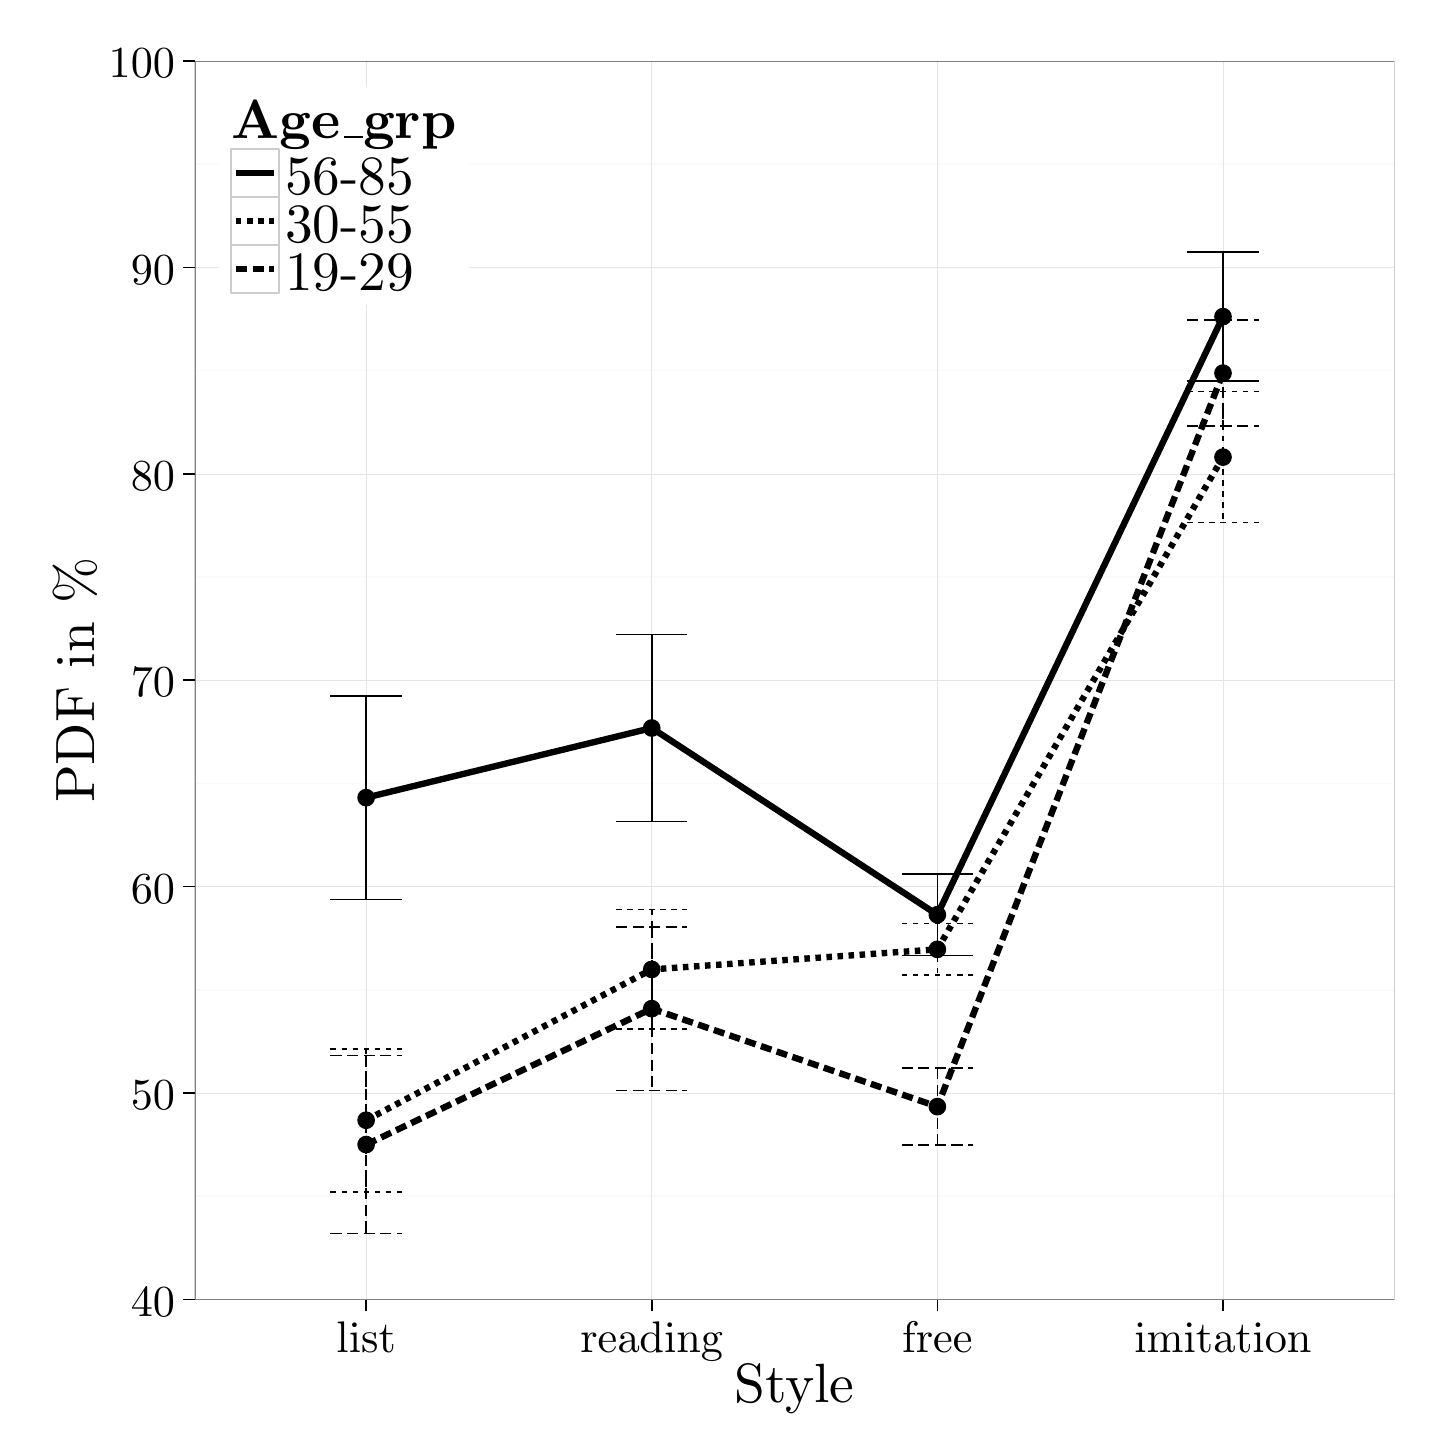
\begin{tikzpicture}[x=1pt,y=1pt]
\definecolor{fillColor}{RGB}{255,255,255}
\path[use as bounding box,fill=fillColor,fill opacity=0.00] (0,0) rectangle (505.89,505.89);
\begin{scope}
\path[clip] (  0.00,  0.00) rectangle (505.89,505.89);
\definecolor{drawColor}{RGB}{255,255,255}
\definecolor{fillColor}{RGB}{255,255,255}

\path[draw=drawColor,line width= 0.6pt,line join=round,line cap=round,fill=fillColor] (  0.00, -0.00) rectangle (505.89,505.89);
\end{scope}
\begin{scope}
\path[clip] ( 60.37, 46.31) rectangle (493.85,493.84);
\definecolor{fillColor}{RGB}{255,255,255}

\path[fill=fillColor] ( 60.37, 46.31) rectangle (493.85,493.84);
\definecolor{drawColor}{gray}{0.98}

\path[draw=drawColor,line width= 0.6pt,line join=round] ( 60.37, 83.60) --
	(493.85, 83.60);

\path[draw=drawColor,line width= 0.6pt,line join=round] ( 60.37,158.19) --
	(493.85,158.19);

\path[draw=drawColor,line width= 0.6pt,line join=round] ( 60.37,232.78) --
	(493.85,232.78);

\path[draw=drawColor,line width= 0.6pt,line join=round] ( 60.37,307.37) --
	(493.85,307.37);

\path[draw=drawColor,line width= 0.6pt,line join=round] ( 60.37,381.96) --
	(493.85,381.96);

\path[draw=drawColor,line width= 0.6pt,line join=round] ( 60.37,456.55) --
	(493.85,456.55);
\definecolor{drawColor}{gray}{0.90}

\path[draw=drawColor,line width= 0.2pt,line join=round] ( 60.37, 46.31) --
	(493.85, 46.31);

\path[draw=drawColor,line width= 0.2pt,line join=round] ( 60.37,120.90) --
	(493.85,120.90);

\path[draw=drawColor,line width= 0.2pt,line join=round] ( 60.37,195.49) --
	(493.85,195.49);

\path[draw=drawColor,line width= 0.2pt,line join=round] ( 60.37,270.08) --
	(493.85,270.08);

\path[draw=drawColor,line width= 0.2pt,line join=round] ( 60.37,344.67) --
	(493.85,344.67);

\path[draw=drawColor,line width= 0.2pt,line join=round] ( 60.37,419.26) --
	(493.85,419.26);

\path[draw=drawColor,line width= 0.2pt,line join=round] ( 60.37,493.84) --
	(493.85,493.84);

\path[draw=drawColor,line width= 0.2pt,line join=round] (122.30, 46.31) --
	(122.30,493.84);

\path[draw=drawColor,line width= 0.2pt,line join=round] (225.50, 46.31) --
	(225.50,493.84);

\path[draw=drawColor,line width= 0.2pt,line join=round] (328.71, 46.31) --
	(328.71,493.84);

\path[draw=drawColor,line width= 0.2pt,line join=round] (431.92, 46.31) --
	(431.92,493.84);
\definecolor{fillColor}{RGB}{0,0,0}

\path[fill=fillColor] (122.30,227.66) circle (  3.20);

\path[fill=fillColor] (122.30,111.09) circle (  3.20);

\path[fill=fillColor] (122.30,102.30) circle (  3.20);

\path[fill=fillColor] (225.50,252.81) circle (  3.20);

\path[fill=fillColor] (225.50,165.59) circle (  3.20);

\path[fill=fillColor] (225.50,151.41) circle (  3.20);

\path[fill=fillColor] (328.71,185.35) circle (  3.20);

\path[fill=fillColor] (328.71,172.84) circle (  3.20);

\path[fill=fillColor] (328.71,116.01) circle (  3.20);

\path[fill=fillColor] (431.92,401.48) circle (  3.20);

\path[fill=fillColor] (431.92,350.71) circle (  3.20);

\path[fill=fillColor] (431.92,381.06) circle (  3.20);
\definecolor{drawColor}{RGB}{0,0,0}

\path[draw=drawColor,line width= 2.3pt,line join=round] (122.30,227.66) --
	(225.50,252.81) --
	(328.71,185.35) --
	(431.92,401.48);

\path[draw=drawColor,line width= 2.3pt,dash pattern=on 2pt off 2pt ,line join=round] (122.30,111.09) --
	(225.50,165.59) --
	(328.71,172.84) --
	(431.92,350.71);

\path[draw=drawColor,line width= 2.3pt,dash pattern=on 4pt off 2pt ,line join=round] (122.30,102.30) --
	(225.50,151.41) --
	(328.71,116.01) --
	(431.92,381.06);

\path[draw=drawColor,line width= 0.6pt,line join=round] (109.40,264.43) --
	(135.20,264.43);

\path[draw=drawColor,line width= 0.6pt,line join=round] (122.30,264.43) --
	(122.30,190.89);

\path[draw=drawColor,line width= 0.6pt,line join=round] (109.40,190.89) --
	(135.20,190.89);

\path[draw=drawColor,line width= 0.6pt,line join=round] (212.60,286.63) --
	(238.41,286.63);

\path[draw=drawColor,line width= 0.6pt,line join=round] (225.50,286.63) --
	(225.50,218.99);

\path[draw=drawColor,line width= 0.6pt,line join=round] (212.60,218.99) --
	(238.41,218.99);

\path[draw=drawColor,line width= 0.6pt,line join=round] (315.81,200.12) --
	(341.61,200.12);

\path[draw=drawColor,line width= 0.6pt,line join=round] (328.71,200.12) --
	(328.71,170.58);

\path[draw=drawColor,line width= 0.6pt,line join=round] (315.81,170.58) --
	(341.61,170.58);

\path[draw=drawColor,line width= 0.6pt,line join=round] (419.02,424.85) --
	(444.82,424.85);

\path[draw=drawColor,line width= 0.6pt,line join=round] (431.92,424.85) --
	(431.92,378.10);

\path[draw=drawColor,line width= 0.6pt,line join=round] (419.02,378.10) --
	(444.82,378.10);

\path[draw=drawColor,line width= 0.6pt,dash pattern=on 2pt off 2pt ,line join=round] (109.40,136.95) --
	(135.20,136.95);

\path[draw=drawColor,line width= 0.6pt,dash pattern=on 2pt off 2pt ,line join=round] (122.30,136.95) --
	(122.30, 85.22);

\path[draw=drawColor,line width= 0.6pt,dash pattern=on 2pt off 2pt ,line join=round] (109.40, 85.22) --
	(135.20, 85.22);

\path[draw=drawColor,line width= 0.6pt,dash pattern=on 2pt off 2pt ,line join=round] (212.60,187.23) --
	(238.41,187.23);

\path[draw=drawColor,line width= 0.6pt,dash pattern=on 2pt off 2pt ,line join=round] (225.50,187.23) --
	(225.50,143.95);

\path[draw=drawColor,line width= 0.6pt,dash pattern=on 2pt off 2pt ,line join=round] (212.60,143.95) --
	(238.41,143.95);

\path[draw=drawColor,line width= 0.6pt,dash pattern=on 2pt off 2pt ,line join=round] (315.81,182.14) --
	(341.61,182.14);

\path[draw=drawColor,line width= 0.6pt,dash pattern=on 2pt off 2pt ,line join=round] (328.71,182.14) --
	(328.71,163.55);

\path[draw=drawColor,line width= 0.6pt,dash pattern=on 2pt off 2pt ,line join=round] (315.81,163.55) --
	(341.61,163.55);

\path[draw=drawColor,line width= 0.6pt,dash pattern=on 2pt off 2pt ,line join=round] (419.02,374.36) --
	(444.82,374.36);

\path[draw=drawColor,line width= 0.6pt,dash pattern=on 2pt off 2pt ,line join=round] (431.92,374.36) --
	(431.92,327.05);

\path[draw=drawColor,line width= 0.6pt,dash pattern=on 2pt off 2pt ,line join=round] (419.02,327.05) --
	(444.82,327.05);

\path[draw=drawColor,line width= 0.6pt,dash pattern=on 4pt off 2pt ,line join=round] (109.40,134.50) --
	(135.20,134.50);

\path[draw=drawColor,line width= 0.6pt,dash pattern=on 4pt off 2pt ,line join=round] (122.30,134.50) --
	(122.30, 70.11);

\path[draw=drawColor,line width= 0.6pt,dash pattern=on 4pt off 2pt ,line join=round] (109.40, 70.11) --
	(135.20, 70.11);

\path[draw=drawColor,line width= 0.6pt,dash pattern=on 4pt off 2pt ,line join=round] (212.60,181.02) --
	(238.41,181.02);

\path[draw=drawColor,line width= 0.6pt,dash pattern=on 4pt off 2pt ,line join=round] (225.50,181.02) --
	(225.50,121.80);

\path[draw=drawColor,line width= 0.6pt,dash pattern=on 4pt off 2pt ,line join=round] (212.60,121.80) --
	(238.41,121.80);

\path[draw=drawColor,line width= 0.6pt,dash pattern=on 4pt off 2pt ,line join=round] (315.81,129.99) --
	(341.61,129.99);

\path[draw=drawColor,line width= 0.6pt,dash pattern=on 4pt off 2pt ,line join=round] (328.71,129.99) --
	(328.71,102.03);

\path[draw=drawColor,line width= 0.6pt,dash pattern=on 4pt off 2pt ,line join=round] (315.81,102.03) --
	(341.61,102.03);

\path[draw=drawColor,line width= 0.6pt,dash pattern=on 4pt off 2pt ,line join=round] (419.02,400.18) --
	(444.82,400.18);

\path[draw=drawColor,line width= 0.6pt,dash pattern=on 4pt off 2pt ,line join=round] (431.92,400.18) --
	(431.92,361.94);

\path[draw=drawColor,line width= 0.6pt,dash pattern=on 4pt off 2pt ,line join=round] (419.02,361.94) --
	(444.82,361.94);
\definecolor{drawColor}{gray}{0.50}

\path[draw=drawColor,line width= 0.6pt,line join=round,line cap=round] ( 60.37, 46.31) rectangle (493.85,493.84);
\end{scope}
\begin{scope}
\path[clip] (  0.00,  0.00) rectangle (505.89,505.89);
\definecolor{drawColor}{RGB}{0,0,0}

\node[text=drawColor,anchor=base east,inner sep=0pt, outer sep=0pt, scale=  1.60] at ( 53.26, 40.27) {40};

\node[text=drawColor,anchor=base east,inner sep=0pt, outer sep=0pt, scale=  1.60] at ( 53.26,114.86) {50};

\node[text=drawColor,anchor=base east,inner sep=0pt, outer sep=0pt, scale=  1.60] at ( 53.26,189.45) {60};

\node[text=drawColor,anchor=base east,inner sep=0pt, outer sep=0pt, scale=  1.60] at ( 53.26,264.04) {70};

\node[text=drawColor,anchor=base east,inner sep=0pt, outer sep=0pt, scale=  1.60] at ( 53.26,338.63) {80};

\node[text=drawColor,anchor=base east,inner sep=0pt, outer sep=0pt, scale=  1.60] at ( 53.26,413.22) {90};

\node[text=drawColor,anchor=base east,inner sep=0pt, outer sep=0pt, scale=  1.60] at ( 53.26,487.81) {100};
\end{scope}
\begin{scope}
\path[clip] (  0.00,  0.00) rectangle (505.89,505.89);
\definecolor{drawColor}{RGB}{0,0,0}

\path[draw=drawColor,line width= 0.6pt,line join=round] ( 56.10, 46.31) --
	( 60.37, 46.31);

\path[draw=drawColor,line width= 0.6pt,line join=round] ( 56.10,120.90) --
	( 60.37,120.90);

\path[draw=drawColor,line width= 0.6pt,line join=round] ( 56.10,195.49) --
	( 60.37,195.49);

\path[draw=drawColor,line width= 0.6pt,line join=round] ( 56.10,270.08) --
	( 60.37,270.08);

\path[draw=drawColor,line width= 0.6pt,line join=round] ( 56.10,344.67) --
	( 60.37,344.67);

\path[draw=drawColor,line width= 0.6pt,line join=round] ( 56.10,419.26) --
	( 60.37,419.26);

\path[draw=drawColor,line width= 0.6pt,line join=round] ( 56.10,493.84) --
	( 60.37,493.84);
\end{scope}
\begin{scope}
\path[clip] (  0.00,  0.00) rectangle (505.89,505.89);
\definecolor{drawColor}{RGB}{0,0,0}

\path[draw=drawColor,line width= 0.6pt,line join=round] (122.30, 42.04) --
	(122.30, 46.31);

\path[draw=drawColor,line width= 0.6pt,line join=round] (225.50, 42.04) --
	(225.50, 46.31);

\path[draw=drawColor,line width= 0.6pt,line join=round] (328.71, 42.04) --
	(328.71, 46.31);

\path[draw=drawColor,line width= 0.6pt,line join=round] (431.92, 42.04) --
	(431.92, 46.31);
\end{scope}
\begin{scope}
\path[clip] (  0.00,  0.00) rectangle (505.89,505.89);
\definecolor{drawColor}{RGB}{0,0,0}

\node[text=drawColor,anchor=base,inner sep=0pt, outer sep=0pt, scale=  1.60] at (122.30, 27.13) {list};

\node[text=drawColor,anchor=base,inner sep=0pt, outer sep=0pt, scale=  1.60] at (225.50, 27.13) {reading};

\node[text=drawColor,anchor=base,inner sep=0pt, outer sep=0pt, scale=  1.60] at (328.71, 27.13) {free};

\node[text=drawColor,anchor=base,inner sep=0pt, outer sep=0pt, scale=  1.60] at (431.92, 27.13) {imitation};
\end{scope}
\begin{scope}
\path[clip] (  0.00,  0.00) rectangle (505.89,505.89);
\definecolor{drawColor}{RGB}{0,0,0}

\node[text=drawColor,anchor=base,inner sep=0pt, outer sep=0pt, scale=  2.00] at (277.11,  9.03) {Style};
\end{scope}
\begin{scope}
\path[clip] (  0.00,  0.00) rectangle (505.89,505.89);
\definecolor{drawColor}{RGB}{0,0,0}

\node[text=drawColor,rotate= 90.00,anchor=base,inner sep=0pt, outer sep=0pt, scale=  2.00] at ( 24.12,270.08) {PDF in {\%}};
\end{scope}
\begin{scope}
\path[clip] (  0.00,  0.00) rectangle (505.89,505.89);
\definecolor{fillColor}{RGB}{255,255,255}

\path[fill=fillColor] ( 69.24,405.66) rectangle (159.40,484.98);
\end{scope}
\begin{scope}
\path[clip] (  0.00,  0.00) rectangle (505.89,505.89);
\definecolor{drawColor}{RGB}{0,0,0}

\node[text=drawColor,anchor=base west,inner sep=0pt, outer sep=0pt, scale=  2.00] at ( 73.51,465.96) {\bfseries Age{\_{}}grp};
\end{scope}
\begin{scope}
\path[clip] (  0.00,  0.00) rectangle (505.89,505.89);
\definecolor{drawColor}{gray}{0.80}
\definecolor{fillColor}{RGB}{255,255,255}

\path[draw=drawColor,line width= 0.6pt,line join=round,line cap=round,fill=fillColor] ( 73.51,444.61) rectangle ( 90.85,461.96);
\end{scope}
\begin{scope}
\path[clip] (  0.00,  0.00) rectangle (505.89,505.89);
\definecolor{drawColor}{RGB}{0,0,0}

\path[draw=drawColor,line width= 2.3pt,line join=round] ( 75.24,453.29) -- ( 89.12,453.29);
\end{scope}
\begin{scope}
\path[clip] (  0.00,  0.00) rectangle (505.89,505.89);
\definecolor{drawColor}{RGB}{0,0,0}

\path[draw=drawColor,line width= 0.6pt,line join=round] ( 75.24,453.29) -- ( 89.12,453.29);
\end{scope}
\begin{scope}
\path[clip] (  0.00,  0.00) rectangle (505.89,505.89);
\definecolor{drawColor}{gray}{0.80}
\definecolor{fillColor}{RGB}{255,255,255}

\path[draw=drawColor,line width= 0.6pt,line join=round,line cap=round,fill=fillColor] ( 73.51,427.27) rectangle ( 90.85,444.61);
\end{scope}
\begin{scope}
\path[clip] (  0.00,  0.00) rectangle (505.89,505.89);
\definecolor{drawColor}{RGB}{0,0,0}

\path[draw=drawColor,line width= 2.3pt,dash pattern=on 2pt off 2pt ,line join=round] ( 75.24,435.94) -- ( 89.12,435.94);
\end{scope}
\begin{scope}
\path[clip] (  0.00,  0.00) rectangle (505.89,505.89);
\definecolor{drawColor}{RGB}{0,0,0}

\path[draw=drawColor,line width= 0.6pt,dash pattern=on 2pt off 2pt ,line join=round] ( 75.24,435.94) -- ( 89.12,435.94);
\end{scope}
\begin{scope}
\path[clip] (  0.00,  0.00) rectangle (505.89,505.89);
\definecolor{drawColor}{gray}{0.80}
\definecolor{fillColor}{RGB}{255,255,255}

\path[draw=drawColor,line width= 0.6pt,line join=round,line cap=round,fill=fillColor] ( 73.51,409.92) rectangle ( 90.85,427.27);
\end{scope}
\begin{scope}
\path[clip] (  0.00,  0.00) rectangle (505.89,505.89);
\definecolor{drawColor}{RGB}{0,0,0}

\path[draw=drawColor,line width= 2.3pt,dash pattern=on 4pt off 2pt ,line join=round] ( 75.24,418.60) -- ( 89.12,418.60);
\end{scope}
\begin{scope}
\path[clip] (  0.00,  0.00) rectangle (505.89,505.89);
\definecolor{drawColor}{RGB}{0,0,0}

\path[draw=drawColor,line width= 0.6pt,dash pattern=on 4pt off 2pt ,line join=round] ( 75.24,418.60) -- ( 89.12,418.60);
\end{scope}
\begin{scope}
\path[clip] (  0.00,  0.00) rectangle (505.89,505.89);
\definecolor{drawColor}{RGB}{0,0,0}

\node[text=drawColor,anchor=base west,inner sep=0pt, outer sep=0pt, scale=  2.00] at ( 93.02,445.75) {56-85};
\end{scope}
\begin{scope}
\path[clip] (  0.00,  0.00) rectangle (505.89,505.89);
\definecolor{drawColor}{RGB}{0,0,0}

\node[text=drawColor,anchor=base west,inner sep=0pt, outer sep=0pt, scale=  2.00] at ( 93.02,428.40) {30-55};
\end{scope}
\begin{scope}
\path[clip] (  0.00,  0.00) rectangle (505.89,505.89);
\definecolor{drawColor}{RGB}{0,0,0}

\node[text=drawColor,anchor=base west,inner sep=0pt, outer sep=0pt, scale=  2.00] at ( 93.02,411.06) {19-29};
\end{scope}
\end{tikzpicture}
} 
		\caption{middle class}
		\label{fig.line.k.mc}
	\end{subfigure}
	\begin{subfigure}{.49\textwidth}
		\centering
			\definecolor{shadecolor}{rgb}{0.969, 0.969, 0.969}
			\resizebox{\linewidth}{!}{% Created by tikzDevice version 0.8.1 on 2016-02-09 02:17:41
% !TEX encoding = UTF-8 Unicode
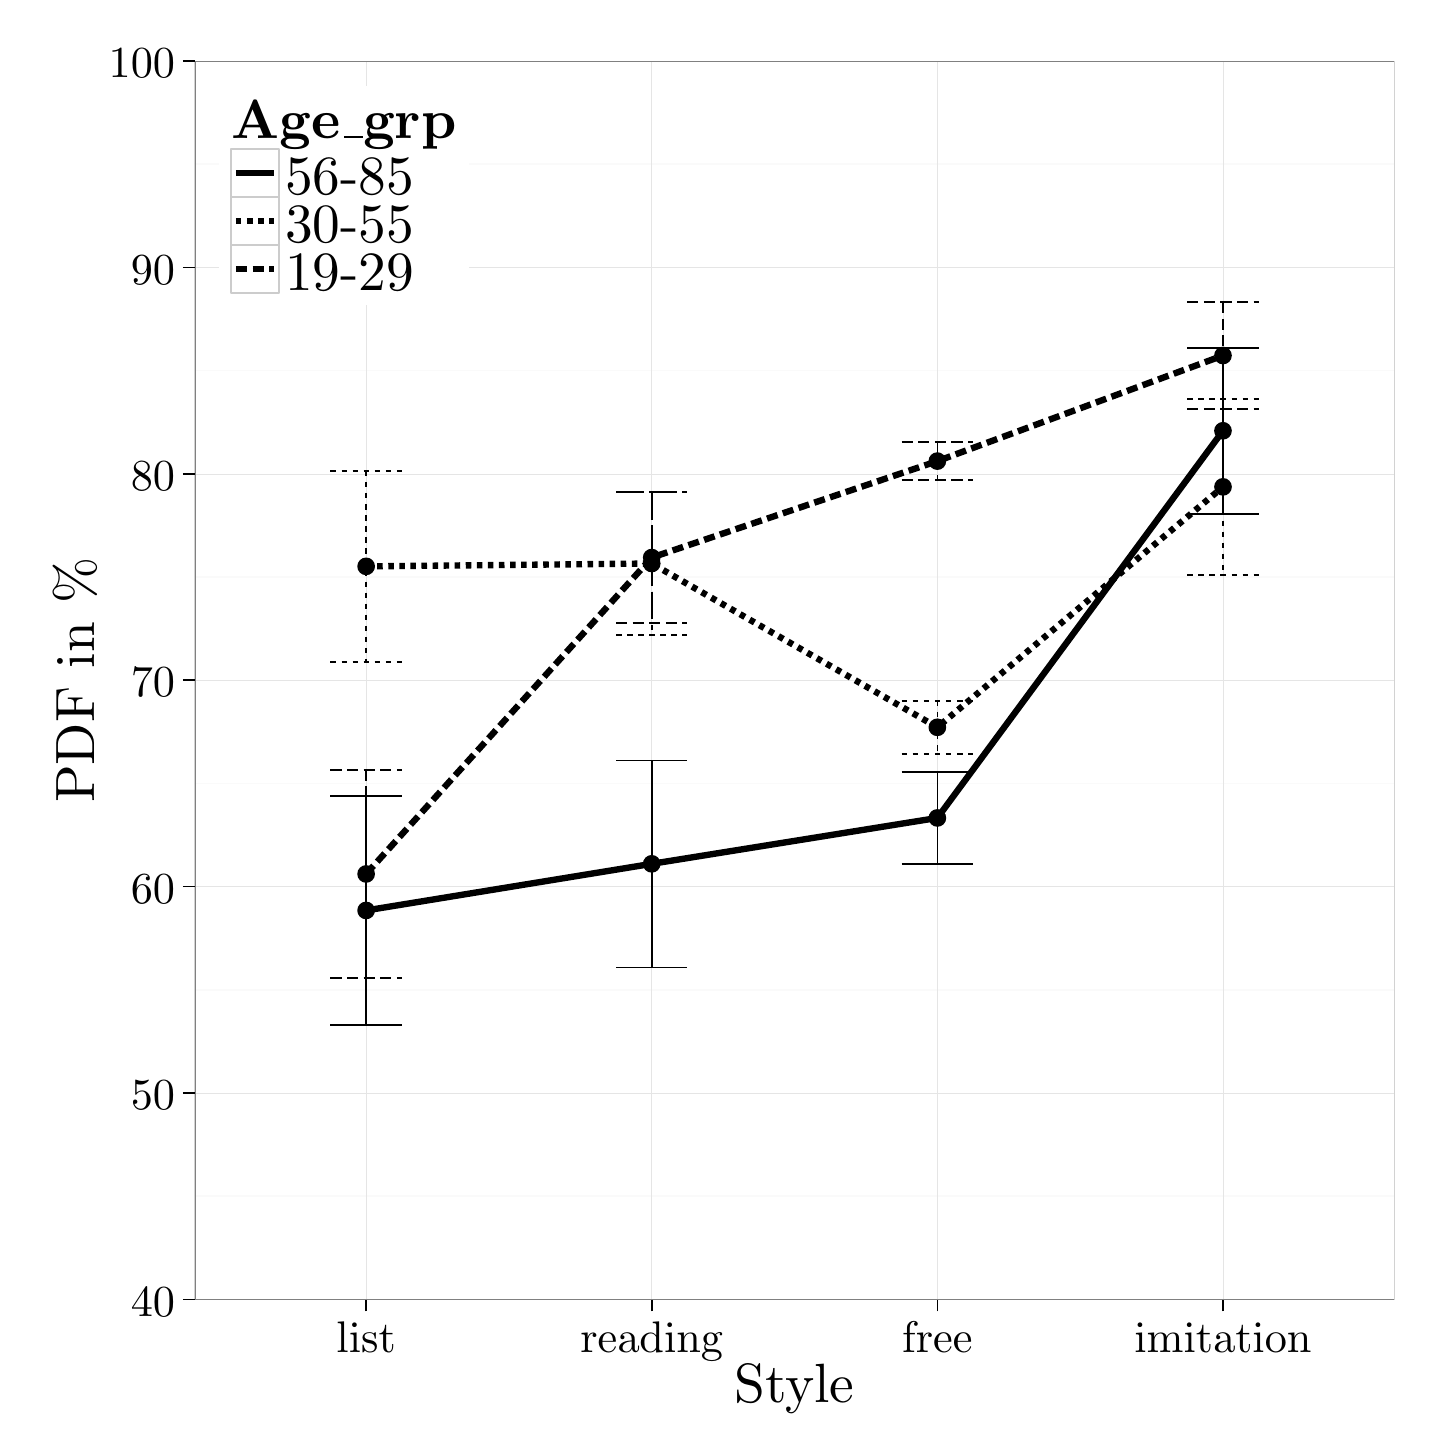
\begin{tikzpicture}[x=1pt,y=1pt]
\definecolor{fillColor}{RGB}{255,255,255}
\path[use as bounding box,fill=fillColor,fill opacity=0.00] (0,0) rectangle (505.89,505.89);
\begin{scope}
\path[clip] (  0.00,  0.00) rectangle (505.89,505.89);
\definecolor{drawColor}{RGB}{255,255,255}
\definecolor{fillColor}{RGB}{255,255,255}

\path[draw=drawColor,line width= 0.6pt,line join=round,line cap=round,fill=fillColor] (  0.00, -0.00) rectangle (505.89,505.89);
\end{scope}
\begin{scope}
\path[clip] ( 60.37, 46.31) rectangle (493.85,493.84);
\definecolor{fillColor}{RGB}{255,255,255}

\path[fill=fillColor] ( 60.37, 46.31) rectangle (493.85,493.84);
\definecolor{drawColor}{gray}{0.98}

\path[draw=drawColor,line width= 0.6pt,line join=round] ( 60.37, 83.60) --
	(493.85, 83.60);

\path[draw=drawColor,line width= 0.6pt,line join=round] ( 60.37,158.19) --
	(493.85,158.19);

\path[draw=drawColor,line width= 0.6pt,line join=round] ( 60.37,232.78) --
	(493.85,232.78);

\path[draw=drawColor,line width= 0.6pt,line join=round] ( 60.37,307.37) --
	(493.85,307.37);

\path[draw=drawColor,line width= 0.6pt,line join=round] ( 60.37,381.96) --
	(493.85,381.96);

\path[draw=drawColor,line width= 0.6pt,line join=round] ( 60.37,456.55) --
	(493.85,456.55);
\definecolor{drawColor}{gray}{0.90}

\path[draw=drawColor,line width= 0.2pt,line join=round] ( 60.37, 46.31) --
	(493.85, 46.31);

\path[draw=drawColor,line width= 0.2pt,line join=round] ( 60.37,120.90) --
	(493.85,120.90);

\path[draw=drawColor,line width= 0.2pt,line join=round] ( 60.37,195.49) --
	(493.85,195.49);

\path[draw=drawColor,line width= 0.2pt,line join=round] ( 60.37,270.08) --
	(493.85,270.08);

\path[draw=drawColor,line width= 0.2pt,line join=round] ( 60.37,344.67) --
	(493.85,344.67);

\path[draw=drawColor,line width= 0.2pt,line join=round] ( 60.37,419.26) --
	(493.85,419.26);

\path[draw=drawColor,line width= 0.2pt,line join=round] ( 60.37,493.84) --
	(493.85,493.84);

\path[draw=drawColor,line width= 0.2pt,line join=round] (122.30, 46.31) --
	(122.30,493.84);

\path[draw=drawColor,line width= 0.2pt,line join=round] (225.50, 46.31) --
	(225.50,493.84);

\path[draw=drawColor,line width= 0.2pt,line join=round] (328.71, 46.31) --
	(328.71,493.84);

\path[draw=drawColor,line width= 0.2pt,line join=round] (431.92, 46.31) --
	(431.92,493.84);
\definecolor{fillColor}{RGB}{0,0,0}

\path[fill=fillColor] (122.30,186.90) circle (  3.20);

\path[fill=fillColor] (122.30,311.23) circle (  3.20);

\path[fill=fillColor] (122.30,200.08) circle (  3.20);

\path[fill=fillColor] (225.50,203.74) circle (  3.20);

\path[fill=fillColor] (225.50,312.26) circle (  3.20);

\path[fill=fillColor] (225.50,314.41) circle (  3.20);

\path[fill=fillColor] (328.71,220.32) circle (  3.20);

\path[fill=fillColor] (328.71,253.07) circle (  3.20);

\path[fill=fillColor] (328.71,349.26) circle (  3.20);

\path[fill=fillColor] (431.92,360.22) circle (  3.20);

\path[fill=fillColor] (431.92,339.96) circle (  3.20);

\path[fill=fillColor] (431.92,387.41) circle (  3.20);
\definecolor{drawColor}{RGB}{0,0,0}

\path[draw=drawColor,line width= 2.3pt,line join=round] (122.30,186.90) --
	(225.50,203.74) --
	(328.71,220.32) --
	(431.92,360.22);

\path[draw=drawColor,line width= 2.3pt,dash pattern=on 2pt off 2pt ,line join=round] (122.30,311.23) --
	(225.50,312.26) --
	(328.71,253.07) --
	(431.92,339.96);

\path[draw=drawColor,line width= 2.3pt,dash pattern=on 4pt off 2pt ,line join=round] (122.30,200.08) --
	(225.50,314.41) --
	(328.71,349.26) --
	(431.92,387.41);

\path[draw=drawColor,line width= 0.6pt,line join=round] (109.40,228.27) --
	(135.20,228.27);

\path[draw=drawColor,line width= 0.6pt,line join=round] (122.30,228.27) --
	(122.30,145.54);

\path[draw=drawColor,line width= 0.6pt,line join=round] (109.40,145.54) --
	(135.20,145.54);

\path[draw=drawColor,line width= 0.6pt,line join=round] (212.60,241.14) --
	(238.41,241.14);

\path[draw=drawColor,line width= 0.6pt,line join=round] (225.50,241.14) --
	(225.50,166.33);

\path[draw=drawColor,line width= 0.6pt,line join=round] (212.60,166.33) --
	(238.41,166.33);

\path[draw=drawColor,line width= 0.6pt,line join=round] (315.81,236.84) --
	(341.61,236.84);

\path[draw=drawColor,line width= 0.6pt,line join=round] (328.71,236.84) --
	(328.71,203.79);

\path[draw=drawColor,line width= 0.6pt,line join=round] (315.81,203.79) --
	(341.61,203.79);

\path[draw=drawColor,line width= 0.6pt,line join=round] (419.02,390.22) --
	(444.82,390.22);

\path[draw=drawColor,line width= 0.6pt,line join=round] (431.92,390.22) --
	(431.92,330.21);

\path[draw=drawColor,line width= 0.6pt,line join=round] (419.02,330.21) --
	(444.82,330.21);

\path[draw=drawColor,line width= 0.6pt,dash pattern=on 2pt off 2pt ,line join=round] (109.40,345.76) --
	(135.20,345.76);

\path[draw=drawColor,line width= 0.6pt,dash pattern=on 2pt off 2pt ,line join=round] (122.30,345.76) --
	(122.30,276.70);

\path[draw=drawColor,line width= 0.6pt,dash pattern=on 2pt off 2pt ,line join=round] (109.40,276.70) --
	(135.20,276.70);

\path[draw=drawColor,line width= 0.6pt,dash pattern=on 2pt off 2pt ,line join=round] (212.60,338.06) --
	(238.41,338.06);

\path[draw=drawColor,line width= 0.6pt,dash pattern=on 2pt off 2pt ,line join=round] (225.50,338.06) --
	(225.50,286.46);

\path[draw=drawColor,line width= 0.6pt,dash pattern=on 2pt off 2pt ,line join=round] (212.60,286.46) --
	(238.41,286.46);

\path[draw=drawColor,line width= 0.6pt,dash pattern=on 2pt off 2pt ,line join=round] (315.81,262.68) --
	(341.61,262.68);

\path[draw=drawColor,line width= 0.6pt,dash pattern=on 2pt off 2pt ,line join=round] (328.71,262.68) --
	(328.71,243.46);

\path[draw=drawColor,line width= 0.6pt,dash pattern=on 2pt off 2pt ,line join=round] (315.81,243.46) --
	(341.61,243.46);

\path[draw=drawColor,line width= 0.6pt,dash pattern=on 2pt off 2pt ,line join=round] (419.02,371.79) --
	(444.82,371.79);

\path[draw=drawColor,line width= 0.6pt,dash pattern=on 2pt off 2pt ,line join=round] (431.92,371.79) --
	(431.92,308.12);

\path[draw=drawColor,line width= 0.6pt,dash pattern=on 2pt off 2pt ,line join=round] (419.02,308.12) --
	(444.82,308.12);

\path[draw=drawColor,line width= 0.6pt,dash pattern=on 4pt off 2pt ,line join=round] (109.40,237.69) --
	(135.20,237.69);

\path[draw=drawColor,line width= 0.6pt,dash pattern=on 4pt off 2pt ,line join=round] (122.30,237.69) --
	(122.30,162.47);

\path[draw=drawColor,line width= 0.6pt,dash pattern=on 4pt off 2pt ,line join=round] (109.40,162.47) --
	(135.20,162.47);

\path[draw=drawColor,line width= 0.6pt,dash pattern=on 4pt off 2pt ,line join=round] (212.60,338.06) --
	(238.41,338.06);

\path[draw=drawColor,line width= 0.6pt,dash pattern=on 4pt off 2pt ,line join=round] (225.50,338.06) --
	(225.50,290.76);

\path[draw=drawColor,line width= 0.6pt,dash pattern=on 4pt off 2pt ,line join=round] (212.60,290.76) --
	(238.41,290.76);

\path[draw=drawColor,line width= 0.6pt,dash pattern=on 4pt off 2pt ,line join=round] (315.81,356.20) --
	(341.61,356.20);

\path[draw=drawColor,line width= 0.6pt,dash pattern=on 4pt off 2pt ,line join=round] (328.71,356.20) --
	(328.71,342.33);

\path[draw=drawColor,line width= 0.6pt,dash pattern=on 4pt off 2pt ,line join=round] (315.81,342.33) --
	(341.61,342.33);

\path[draw=drawColor,line width= 0.6pt,dash pattern=on 4pt off 2pt ,line join=round] (419.02,406.68) --
	(444.82,406.68);

\path[draw=drawColor,line width= 0.6pt,dash pattern=on 4pt off 2pt ,line join=round] (431.92,406.68) --
	(431.92,368.15);

\path[draw=drawColor,line width= 0.6pt,dash pattern=on 4pt off 2pt ,line join=round] (419.02,368.15) --
	(444.82,368.15);
\definecolor{drawColor}{gray}{0.50}

\path[draw=drawColor,line width= 0.6pt,line join=round,line cap=round] ( 60.37, 46.31) rectangle (493.85,493.84);
\end{scope}
\begin{scope}
\path[clip] (  0.00,  0.00) rectangle (505.89,505.89);
\definecolor{drawColor}{RGB}{0,0,0}

\node[text=drawColor,anchor=base east,inner sep=0pt, outer sep=0pt, scale=  1.60] at ( 53.26, 40.27) {40};

\node[text=drawColor,anchor=base east,inner sep=0pt, outer sep=0pt, scale=  1.60] at ( 53.26,114.86) {50};

\node[text=drawColor,anchor=base east,inner sep=0pt, outer sep=0pt, scale=  1.60] at ( 53.26,189.45) {60};

\node[text=drawColor,anchor=base east,inner sep=0pt, outer sep=0pt, scale=  1.60] at ( 53.26,264.04) {70};

\node[text=drawColor,anchor=base east,inner sep=0pt, outer sep=0pt, scale=  1.60] at ( 53.26,338.63) {80};

\node[text=drawColor,anchor=base east,inner sep=0pt, outer sep=0pt, scale=  1.60] at ( 53.26,413.22) {90};

\node[text=drawColor,anchor=base east,inner sep=0pt, outer sep=0pt, scale=  1.60] at ( 53.26,487.81) {100};
\end{scope}
\begin{scope}
\path[clip] (  0.00,  0.00) rectangle (505.89,505.89);
\definecolor{drawColor}{RGB}{0,0,0}

\path[draw=drawColor,line width= 0.6pt,line join=round] ( 56.10, 46.31) --
	( 60.37, 46.31);

\path[draw=drawColor,line width= 0.6pt,line join=round] ( 56.10,120.90) --
	( 60.37,120.90);

\path[draw=drawColor,line width= 0.6pt,line join=round] ( 56.10,195.49) --
	( 60.37,195.49);

\path[draw=drawColor,line width= 0.6pt,line join=round] ( 56.10,270.08) --
	( 60.37,270.08);

\path[draw=drawColor,line width= 0.6pt,line join=round] ( 56.10,344.67) --
	( 60.37,344.67);

\path[draw=drawColor,line width= 0.6pt,line join=round] ( 56.10,419.26) --
	( 60.37,419.26);

\path[draw=drawColor,line width= 0.6pt,line join=round] ( 56.10,493.84) --
	( 60.37,493.84);
\end{scope}
\begin{scope}
\path[clip] (  0.00,  0.00) rectangle (505.89,505.89);
\definecolor{drawColor}{RGB}{0,0,0}

\path[draw=drawColor,line width= 0.6pt,line join=round] (122.30, 42.04) --
	(122.30, 46.31);

\path[draw=drawColor,line width= 0.6pt,line join=round] (225.50, 42.04) --
	(225.50, 46.31);

\path[draw=drawColor,line width= 0.6pt,line join=round] (328.71, 42.04) --
	(328.71, 46.31);

\path[draw=drawColor,line width= 0.6pt,line join=round] (431.92, 42.04) --
	(431.92, 46.31);
\end{scope}
\begin{scope}
\path[clip] (  0.00,  0.00) rectangle (505.89,505.89);
\definecolor{drawColor}{RGB}{0,0,0}

\node[text=drawColor,anchor=base,inner sep=0pt, outer sep=0pt, scale=  1.60] at (122.30, 27.13) {list};

\node[text=drawColor,anchor=base,inner sep=0pt, outer sep=0pt, scale=  1.60] at (225.50, 27.13) {reading};

\node[text=drawColor,anchor=base,inner sep=0pt, outer sep=0pt, scale=  1.60] at (328.71, 27.13) {free};

\node[text=drawColor,anchor=base,inner sep=0pt, outer sep=0pt, scale=  1.60] at (431.92, 27.13) {imitation};
\end{scope}
\begin{scope}
\path[clip] (  0.00,  0.00) rectangle (505.89,505.89);
\definecolor{drawColor}{RGB}{0,0,0}

\node[text=drawColor,anchor=base,inner sep=0pt, outer sep=0pt, scale=  2.00] at (277.11,  9.03) {Style};
\end{scope}
\begin{scope}
\path[clip] (  0.00,  0.00) rectangle (505.89,505.89);
\definecolor{drawColor}{RGB}{0,0,0}

\node[text=drawColor,rotate= 90.00,anchor=base,inner sep=0pt, outer sep=0pt, scale=  2.00] at ( 24.12,270.08) {PDF in {\%}};
\end{scope}
\begin{scope}
\path[clip] (  0.00,  0.00) rectangle (505.89,505.89);
\definecolor{fillColor}{RGB}{255,255,255}

\path[fill=fillColor] ( 69.24,405.66) rectangle (159.40,484.98);
\end{scope}
\begin{scope}
\path[clip] (  0.00,  0.00) rectangle (505.89,505.89);
\definecolor{drawColor}{RGB}{0,0,0}

\node[text=drawColor,anchor=base west,inner sep=0pt, outer sep=0pt, scale=  2.00] at ( 73.51,465.96) {\bfseries Age{\_{}}grp};
\end{scope}
\begin{scope}
\path[clip] (  0.00,  0.00) rectangle (505.89,505.89);
\definecolor{drawColor}{gray}{0.80}
\definecolor{fillColor}{RGB}{255,255,255}

\path[draw=drawColor,line width= 0.6pt,line join=round,line cap=round,fill=fillColor] ( 73.51,444.61) rectangle ( 90.85,461.96);
\end{scope}
\begin{scope}
\path[clip] (  0.00,  0.00) rectangle (505.89,505.89);
\definecolor{drawColor}{RGB}{0,0,0}

\path[draw=drawColor,line width= 2.3pt,line join=round] ( 75.24,453.29) -- ( 89.12,453.29);
\end{scope}
\begin{scope}
\path[clip] (  0.00,  0.00) rectangle (505.89,505.89);
\definecolor{drawColor}{RGB}{0,0,0}

\path[draw=drawColor,line width= 0.6pt,line join=round] ( 75.24,453.29) -- ( 89.12,453.29);
\end{scope}
\begin{scope}
\path[clip] (  0.00,  0.00) rectangle (505.89,505.89);
\definecolor{drawColor}{gray}{0.80}
\definecolor{fillColor}{RGB}{255,255,255}

\path[draw=drawColor,line width= 0.6pt,line join=round,line cap=round,fill=fillColor] ( 73.51,427.27) rectangle ( 90.85,444.61);
\end{scope}
\begin{scope}
\path[clip] (  0.00,  0.00) rectangle (505.89,505.89);
\definecolor{drawColor}{RGB}{0,0,0}

\path[draw=drawColor,line width= 2.3pt,dash pattern=on 2pt off 2pt ,line join=round] ( 75.24,435.94) -- ( 89.12,435.94);
\end{scope}
\begin{scope}
\path[clip] (  0.00,  0.00) rectangle (505.89,505.89);
\definecolor{drawColor}{RGB}{0,0,0}

\path[draw=drawColor,line width= 0.6pt,dash pattern=on 2pt off 2pt ,line join=round] ( 75.24,435.94) -- ( 89.12,435.94);
\end{scope}
\begin{scope}
\path[clip] (  0.00,  0.00) rectangle (505.89,505.89);
\definecolor{drawColor}{gray}{0.80}
\definecolor{fillColor}{RGB}{255,255,255}

\path[draw=drawColor,line width= 0.6pt,line join=round,line cap=round,fill=fillColor] ( 73.51,409.92) rectangle ( 90.85,427.27);
\end{scope}
\begin{scope}
\path[clip] (  0.00,  0.00) rectangle (505.89,505.89);
\definecolor{drawColor}{RGB}{0,0,0}

\path[draw=drawColor,line width= 2.3pt,dash pattern=on 4pt off 2pt ,line join=round] ( 75.24,418.60) -- ( 89.12,418.60);
\end{scope}
\begin{scope}
\path[clip] (  0.00,  0.00) rectangle (505.89,505.89);
\definecolor{drawColor}{RGB}{0,0,0}

\path[draw=drawColor,line width= 0.6pt,dash pattern=on 4pt off 2pt ,line join=round] ( 75.24,418.60) -- ( 89.12,418.60);
\end{scope}
\begin{scope}
\path[clip] (  0.00,  0.00) rectangle (505.89,505.89);
\definecolor{drawColor}{RGB}{0,0,0}

\node[text=drawColor,anchor=base west,inner sep=0pt, outer sep=0pt, scale=  2.00] at ( 93.02,445.75) {56-85};
\end{scope}
\begin{scope}
\path[clip] (  0.00,  0.00) rectangle (505.89,505.89);
\definecolor{drawColor}{RGB}{0,0,0}

\node[text=drawColor,anchor=base west,inner sep=0pt, outer sep=0pt, scale=  2.00] at ( 93.02,428.40) {30-55};
\end{scope}
\begin{scope}
\path[clip] (  0.00,  0.00) rectangle (505.89,505.89);
\definecolor{drawColor}{RGB}{0,0,0}

\node[text=drawColor,anchor=base west,inner sep=0pt, outer sep=0pt, scale=  2.00] at ( 93.02,411.06) {19-29};
\end{scope}
\end{tikzpicture}
} 
		\caption{working class}
		\label{fig.line.k.wc}
	\end{subfigure}
	\caption{/k/: PDF by style, age group, and social class (released only)}
\end{figure}

In \figref{fig.line.k.mc} and \figref{fig.line.k.wc} the style-age interaction is shown with respect to how it is influenced by social class of the speaker.
For old middle-class speakers (solid line in \figref{fig.line.k.mc}) we find again that there is no significant difference between the word list and the text reading task.
The, by now familiar, steep rise to a very high \isi{PDF} for accent imitation\is{accent performance} is also present.
In between, however, /k/ variants become more standard in free speech -- \isi{PDF} drops.
While the difference between realisations in spontaneous speech and while reading out the word list is not statistically robust, that between free speech and the text passage is.
Old working-class speakers behave in very much the same way as the pooled age group in \figref{fig.line.k.tot}: `list', `reading', and `free' are not significantly different, but there is a steep and statistically robust increase of \isi{PDF} during accent imitation\is{accent performance}.

Middle-class speakers aged between 30 and 55 show exactly the same \isi{style shifting} pattern that was found for young male subjects (cf. \figref{fig.line.k.mal}).
The reading passage and spontaneous speech are statistically identical, but apart from that, there is a steady increase in \isi{PDF} from left (more formal) to right (less formal).
Their working-class counterparts (dotted line in \figref{fig.line.k.wc}) are interesting because they echo the phenomenon just described for old middle-class speakers: `list' and `reading' are identical, followed by a significant drop in \isi{PDF} towards spontaneous speech, and then by a significant rise for accent imitation\is{accent performance}.
The only difference is that for middle-aged working-class speakers /k/ realisations in the word list and the reading passage are just as Scouse as when people put on a particularly strong Liverpool accent.

Young middle-class participants, finally, exhibit a style pattern which looks like an attenuated version of the one revealed for old middle-class speakers.
In this age group, however, the drop in \isi{PDF} from `reading' to `free' is not significant.
As a result, the three styles word list, reading passage, and spontaneous speech are all identical, statistically speaking.
The following increase in \isi{PDF} during accent perform\is{accent performance}ance is then even (slightly) more extreme than for the other two age groups.
Somewhat surprisingly, working-class speakers (dashed line in \figref{fig.line.k.wc}) do distinguish all four styles.
Not only is each of them significantly different from each of the other three, but there is also a steady increase in \isi{PDF} from left to right -- just as one would expect for a socially salient\is{salience} variable that people are aware\is{awareness} of to a certain degree.
We are thus faced with the interesting situation that, among the youngest subjects, it is actually the working-class speakers who exhibit more pronounced and more systematic \isi{style shifting}.
It should be noted, however, that this might just be due to the fact that young middle-class speakers have considerably lower \isi{PDF} values than working-class Liverpudlians of the same age in the first three styles; young middle-class speakers might just try not to use /k/ lenition at all (as far as they are able to do so, cf. \sectref{aware_res.phon.k}), irrespective of speaking style, unless they are told to do so.